\documentclass[twoside]{book}

% Packages required by doxygen
\usepackage{calc}
\usepackage{doxygen}
\usepackage{graphicx}
\usepackage[utf8]{inputenc}
\usepackage{makeidx}
\usepackage{multicol}
\usepackage{multirow}
\usepackage{textcomp}
\usepackage[table]{xcolor}

% Font selection
\usepackage[T1]{fontenc}
\usepackage{mathptmx}
\usepackage[scaled=.90]{helvet}
\usepackage{courier}
\usepackage{amssymb}
\usepackage{sectsty}
\renewcommand{\familydefault}{\sfdefault}
\allsectionsfont{%
  \fontseries{bc}\selectfont%
  \color{darkgray}%
}
\renewcommand{\DoxyLabelFont}{%
  \fontseries{bc}\selectfont%
  \color{darkgray}%
}

% Page & text layout
\usepackage{geometry}
\geometry{%
  a4paper,%
  top=2.5cm,%
  bottom=2.5cm,%
  left=2.5cm,%
  right=2.5cm%
}
\tolerance=750
\hfuzz=15pt
\hbadness=750
\setlength{\emergencystretch}{15pt}
\setlength{\parindent}{0cm}
\setlength{\parskip}{0.2cm}
\makeatletter
\renewcommand{\paragraph}{%
  \@startsection{paragraph}{4}{0ex}{-1.0ex}{1.0ex}{%
    \normalfont\normalsize\bfseries\SS@parafont%
  }%
}
\renewcommand{\subparagraph}{%
  \@startsection{subparagraph}{5}{0ex}{-1.0ex}{1.0ex}{%
    \normalfont\normalsize\bfseries\SS@subparafont%
  }%
}
\makeatother

% Headers & footers
\usepackage{fancyhdr}
\pagestyle{fancyplain}
\fancyhead[LE]{\fancyplain{}{\bfseries\thepage}}
\fancyhead[CE]{\fancyplain{}{}}
\fancyhead[RE]{\fancyplain{}{\bfseries\leftmark}}
\fancyhead[LO]{\fancyplain{}{\bfseries\rightmark}}
\fancyhead[CO]{\fancyplain{}{}}
\fancyhead[RO]{\fancyplain{}{\bfseries\thepage}}
\fancyfoot[LE]{\fancyplain{}{}}
\fancyfoot[CE]{\fancyplain{}{}}
\fancyfoot[RE]{\fancyplain{}{\bfseries\scriptsize Generated on Tue Apr 19 2016 17\-:15\-:19 for Ophidian by Doxygen }}
\fancyfoot[LO]{\fancyplain{}{\bfseries\scriptsize Generated on Tue Apr 19 2016 17\-:15\-:19 for Ophidian by Doxygen }}
\fancyfoot[CO]{\fancyplain{}{}}
\fancyfoot[RO]{\fancyplain{}{}}
\renewcommand{\footrulewidth}{0.4pt}
\renewcommand{\chaptermark}[1]{%
  \markboth{#1}{}%
}
\renewcommand{\sectionmark}[1]{%
  \markright{\thesection\ #1}%
}

% Indices & bibliography
\usepackage{natbib}
\usepackage[titles]{tocloft}
\setcounter{tocdepth}{3}
\setcounter{secnumdepth}{5}
\makeindex

% Hyperlinks (required, but should be loaded last)
\usepackage{ifpdf}
\ifpdf
  \usepackage[pdftex,pagebackref=true]{hyperref}
\else
  \usepackage[ps2pdf,pagebackref=true]{hyperref}
\fi
\hypersetup{%
  colorlinks=true,%
  linkcolor=blue,%
  citecolor=blue,%
  unicode%
}

% Custom commands
\newcommand{\clearemptydoublepage}{%
  \newpage{\pagestyle{empty}\cleardoublepage}%
}


%===== C O N T E N T S =====

\begin{document}

% Titlepage & ToC
\hypersetup{pageanchor=false}
\pagenumbering{roman}
\begin{titlepage}
\vspace*{7cm}
\begin{center}%
{\Large Ophidian }\\
\vspace*{1cm}
{\large Generated by Doxygen 1.8.6}\\
\vspace*{0.5cm}
{\small Tue Apr 19 2016 17:15:19}\\
\end{center}
\end{titlepage}
\clearemptydoublepage
\tableofcontents
\clearemptydoublepage
\pagenumbering{arabic}
\hypersetup{pageanchor=true}

%--- Begin generated contents ---
\chapter{Namespace Index}
\section{Namespace List}
Here is a list of all documented namespaces with brief descriptions\-:\begin{DoxyCompactList}
\item\contentsline{section}{\hyperlink{namespaceophidian}{ophidian} \\*The namespace of Ophidian }{\pageref{namespaceophidian}}{}
\item\contentsline{section}{\hyperlink{namespaceophidian_1_1density}{ophidian\-::density} \\*Classes and algorithms related to density }{\pageref{namespaceophidian_1_1density}}{}
\item\contentsline{section}{\hyperlink{namespaceophidian_1_1floorplan}{ophidian\-::floorplan} \\*Namespace describing floorplan entities and basic floorplan interface }{\pageref{namespaceophidian_1_1floorplan}}{}
\item\contentsline{section}{\hyperlink{namespaceophidian_1_1interconnection}{ophidian\-::interconnection} \\*The Interonnection namespace }{\pageref{namespaceophidian_1_1interconnection}}{}
\item\contentsline{section}{\hyperlink{namespaceophidian_1_1netlist}{ophidian\-::netlist} \\*Namespace describing netlist entities and basic netlist interface }{\pageref{namespaceophidian_1_1netlist}}{}
\item\contentsline{section}{\hyperlink{namespaceophidian_1_1placement}{ophidian\-::placement} \\*Namespace describing placement entities and basic placement interface }{\pageref{namespaceophidian_1_1placement}}{}
\item\contentsline{section}{\hyperlink{namespaceophidian_1_1routing}{ophidian\-::routing} \\*Namespace describing routing entities and basic routing interface }{\pageref{namespaceophidian_1_1routing}}{}
\item\contentsline{section}{\hyperlink{namespaceophidian_1_1standard__cell}{ophidian\-::standard\-\_\-cell} \\*Namespace describing standard cell entities and basic standard cell interface }{\pageref{namespaceophidian_1_1standard__cell}}{}
\end{DoxyCompactList}

\chapter{Hierarchical Index}
\section{Class Hierarchy}
This inheritance list is sorted roughly, but not completely, alphabetically\-:\begin{DoxyCompactList}
\item \contentsline{section}{ophidian\-:\-:entity\-:\-:bimap\-\_\-iterator\-\_\-adapter}{\pageref{classophidian_1_1entity_1_1bimap__iterator__adapter}}{}
\item \contentsline{section}{ophidian\-:\-:timingdriven\-\_\-placement\-:\-:bounds$<$ Iterator\-Type $>$}{\pageref{structophidian_1_1timingdriven__placement_1_1bounds}}{}
\item \contentsline{section}{ophidian\-:\-:netlist\-:\-:cells}{\pageref{classophidian_1_1netlist_1_1cells}}{}
\item \contentsline{section}{ophidian\-:\-:placement\-:\-:cells}{\pageref{classophidian_1_1placement_1_1cells}}{}
\item \contentsline{section}{ophidian\-:\-:standard\-\_\-cell\-:\-:cells}{\pageref{classophidian_1_1standard__cell_1_1cells}}{}
\item \contentsline{section}{ophidian\-:\-:timingdriven\-\_\-placement\-:\-:cells\-\_\-geometries}{\pageref{structophidian_1_1timingdriven__placement_1_1cells__geometries}}{}
\item \contentsline{section}{ophidian\-:\-:interconnection\-:\-:compare\-\_\-xcoord}{\pageref{classophidian_1_1interconnection_1_1compare__xcoord}}{}
\item \contentsline{section}{ophidian\-:\-:interconnection\-:\-:compare\-\_\-ycoord}{\pageref{classophidian_1_1interconnection_1_1compare__ycoord}}{}
\item \contentsline{section}{ophidian\-:\-:interconnection\-:\-:csoln}{\pageref{structophidian_1_1interconnection_1_1csoln}}{}
\item \contentsline{section}{ophidian\-:\-:timing\-:\-:dc\-\_\-clock}{\pageref{structophidian_1_1timing_1_1dc__clock}}{}
\item \contentsline{section}{ophidian\-:\-:timing\-:\-:dc\-\_\-driving\-\_\-cell}{\pageref{structophidian_1_1timing_1_1dc__driving__cell}}{}
\item \contentsline{section}{ophidian\-:\-:timing\-:\-:dc\-\_\-input\-\_\-delays}{\pageref{structophidian_1_1timing_1_1dc__input__delays}}{}
\item \contentsline{section}{ophidian\-:\-:timing\-:\-:dc\-\_\-output\-\_\-delay}{\pageref{structophidian_1_1timing_1_1dc__output__delay}}{}
\item \contentsline{section}{ophidian\-:\-:timing\-:\-:dc\-\_\-output\-\_\-load}{\pageref{structophidian_1_1timing_1_1dc__output__load}}{}
\item \contentsline{section}{ophidian\-:\-:timing\-:\-:default\-\_\-design\-\_\-constraints}{\pageref{classophidian_1_1timing_1_1default__design__constraints}}{}
\item \contentsline{section}{ophidian\-:\-:timing\-:\-:design\-\_\-constraints}{\pageref{structophidian_1_1timing_1_1design__constraints}}{}
\item \contentsline{section}{ophidian\-:\-:timing\-:\-:effective\-\_\-capacitance\-\_\-wire\-\_\-model}{\pageref{classophidian_1_1timing_1_1effective__capacitance__wire__model}}{}
\item \contentsline{section}{ophidian\-:\-:timing\-:\-:elmore}{\pageref{classophidian_1_1timing_1_1elmore}}{}
\item \contentsline{section}{ophidian\-:\-:timing\-:\-:elmore\-\_\-second\-\_\-moment}{\pageref{classophidian_1_1timing_1_1elmore__second__moment}}{}
\item \contentsline{section}{ophidian\-:\-:timing\-:\-:endpoints}{\pageref{classophidian_1_1timing_1_1endpoints}}{}
\item \contentsline{section}{ophidian\-:\-:entity\-:\-:entity}{\pageref{classophidian_1_1entity_1_1entity}}{}
\item \contentsline{section}{ophidian\-:\-:floorplan\-:\-:floorplan}{\pageref{classophidian_1_1floorplan_1_1floorplan}}{}
\item \contentsline{section}{ophidian\-:\-:timingdriven\-\_\-placement\-:\-:flute\-\_\-rc\-\_\-tree\-\_\-creator}{\pageref{classophidian_1_1timingdriven__placement_1_1flute__rc__tree__creator}}{}
\item \contentsline{section}{ophidian\-:\-:timing\-:\-:generic\-\_\-sta$<$ Wire\-Delay\-Model, Merge\-Strategy $>$}{\pageref{classophidian_1_1timing_1_1generic__sta}}{}
\item \contentsline{section}{ophidian\-:\-:timing\-:\-:graph}{\pageref{classophidian_1_1timing_1_1graph}}{}
\item \contentsline{section}{ophidian\-:\-:timing\-:\-:graph\-\_\-and\-\_\-topology}{\pageref{structophidian_1_1timing_1_1graph__and__topology}}{}
\item \contentsline{section}{ophidian\-:\-:timing\-:\-:graph\-\_\-arcs\-\_\-timing}{\pageref{classophidian_1_1timing_1_1graph__arcs__timing}}{}
\item \contentsline{section}{ophidian\-:\-:timing\-:\-:graph\-\_\-builder}{\pageref{classophidian_1_1timing_1_1graph__builder}}{}
\item \contentsline{section}{ophidian\-:\-:timing\-:\-:graph\-\_\-nodes\-\_\-timing}{\pageref{classophidian_1_1timing_1_1graph__nodes__timing}}{}
\item \contentsline{section}{ophidian\-:\-:placement\-:\-:library}{\pageref{classophidian_1_1placement_1_1library}}{}
\item \contentsline{section}{ophidian\-:\-:timing\-:\-:library}{\pageref{classophidian_1_1timing_1_1library}}{}
\item \contentsline{section}{ophidian\-:\-:placement\-:\-:library\-\_\-pins}{\pageref{classophidian_1_1placement_1_1library__pins}}{}
\item \contentsline{section}{ophidian\-:\-:timing\-:\-:library\-\_\-timing\-\_\-arcs}{\pageref{classophidian_1_1timing_1_1library__timing__arcs}}{}
\item \contentsline{section}{ophidian\-:\-:timing\-:\-:lookup\-\_\-table$<$ Row\-Type, Column\-Type, Value\-Type $>$}{\pageref{classophidian_1_1timing_1_1lookup__table}}{}
\item \contentsline{section}{ophidian\-:\-:timing\-:\-:lumped\-\_\-capacitance\-\_\-wire\-\_\-model}{\pageref{classophidian_1_1timing_1_1lumped__capacitance__wire__model}}{}
\item \contentsline{section}{ophidian\-:\-:netlist\-:\-:netlist}{\pageref{classophidian_1_1netlist_1_1netlist}}{}
\item \contentsline{section}{ophidian\-:\-:netlist\-:\-:nets}{\pageref{classophidian_1_1netlist_1_1nets}}{}
\item \contentsline{section}{ophidian\-:\-:timing\-:\-:optimistic}{\pageref{structophidian_1_1timing_1_1optimistic}}{}
\item \contentsline{section}{ophidian\-:\-:timing\-:\-:pair\-\_\-hash}{\pageref{structophidian_1_1timing_1_1pair__hash}}{}
\item \contentsline{section}{ophidian\-:\-:timing\-:\-:pessimistic}{\pageref{structophidian_1_1timing_1_1pessimistic}}{}
\item \contentsline{section}{ophidian\-:\-:netlist\-:\-:pins}{\pageref{classophidian_1_1netlist_1_1pins}}{}
\item \contentsline{section}{ophidian\-:\-:standard\-\_\-cell\-:\-:pins}{\pageref{classophidian_1_1standard__cell_1_1pins}}{}
\item \contentsline{section}{ophidian\-:\-:placement\-:\-:placement}{\pageref{classophidian_1_1placement_1_1placement}}{}
\item \contentsline{section}{ophidian\-:\-:interconnection\-:\-:point}{\pageref{structophidian_1_1interconnection_1_1point}}{}
\item \contentsline{section}{ophidian\-:\-:entity\-:\-:property}{\pageref{classophidian_1_1entity_1_1property}}{}
\begin{DoxyCompactList}
\item \contentsline{section}{ophidian\-:\-:entity\-:\-:vector\-\_\-property$<$ T $>$}{\pageref{classophidian_1_1entity_1_1vector__property}}{}
\item \contentsline{section}{ophidian\-:\-:entity\-:\-:vector\-\_\-property$<$ bool $>$}{\pageref{classophidian_1_1entity_1_1vector__property_3_01bool_01_4}}{}
\item \contentsline{section}{ophidian\-:\-:entity\-:\-:vector\-\_\-property$<$ boost\-:\-:units\-:\-:quantity$<$ boost\-:\-:units\-:\-:si\-:\-:capacitance $>$ $>$}{\pageref{classophidian_1_1entity_1_1vector__property}}{}
\item \contentsline{section}{ophidian\-:\-:entity\-:\-:vector\-\_\-property$<$ entity\-:\-:entity $>$}{\pageref{classophidian_1_1entity_1_1vector__property}}{}
\item \contentsline{section}{ophidian\-:\-:entity\-:\-:vector\-\_\-property$<$ interconnection\-:\-:ophidian\-:\-:interconnection\-:\-:rc\-\_\-tree $>$}{\pageref{classophidian_1_1entity_1_1vector__property}}{}
\item \contentsline{section}{ophidian\-:\-:entity\-:\-:vector\-\_\-property$<$ interconnection\-:\-:rc\-\_\-tree $>$}{\pageref{classophidian_1_1entity_1_1vector__property}}{}
\item \contentsline{section}{ophidian\-:\-:entity\-:\-:vector\-\_\-property$<$ multipolygon $>$}{\pageref{classophidian_1_1entity_1_1vector__property}}{}
\item \contentsline{section}{ophidian\-:\-:entity\-:\-:vector\-\_\-property$<$ ophidian\-:\-:timing\-:\-:lookup\-\_\-table $>$}{\pageref{classophidian_1_1entity_1_1vector__property}}{}
\item \contentsline{section}{ophidian\-:\-:entity\-:\-:vector\-\_\-property$<$ pin\-\_\-directions $>$}{\pageref{classophidian_1_1entity_1_1vector__property}}{}
\item \contentsline{section}{ophidian\-:\-:entity\-:\-:vector\-\_\-property$<$ point $>$}{\pageref{classophidian_1_1entity_1_1vector__property}}{}
\item \contentsline{section}{ophidian\-:\-:entity\-:\-:vector\-\_\-property$<$ timing\-\_\-arc\-\_\-types $>$}{\pageref{classophidian_1_1entity_1_1vector__property}}{}
\item \contentsline{section}{ophidian\-:\-:entity\-:\-:vector\-\_\-property$<$ unateness $>$}{\pageref{classophidian_1_1entity_1_1vector__property}}{}
\item \contentsline{section}{ophidian\-:\-:entity\-:\-:vector\-\_\-property$<$ unsigned $>$}{\pageref{classophidian_1_1entity_1_1vector__property}}{}
\end{DoxyCompactList}
\item \contentsline{section}{ophidian\-:\-:interconnection\-:\-:rc\-\_\-tree}{\pageref{classophidian_1_1interconnection_1_1rc__tree}}{}
\item \contentsline{section}{ophidian\-:\-:floorplan\-:\-:rows}{\pageref{classophidian_1_1floorplan_1_1rows}}{}
\item \contentsline{section}{ophidian\-:\-:timingdriven\-\_\-placement\-:\-:flute\-\_\-rc\-\_\-tree\-\_\-rtree\-:\-:rtree\-\_\-node\-\_\-comparator}{\pageref{classophidian_1_1timingdriven__placement_1_1flute__rc__tree__rtree_1_1rtree__node__comparator}}{}
\item \contentsline{section}{ophidian\-:\-:timing\-:\-:simple\-\_\-design\-\_\-constraint}{\pageref{classophidian_1_1timing_1_1simple__design__constraint}}{}
\item \contentsline{section}{ophidian\-:\-:floorplan\-:\-:sites}{\pageref{classophidian_1_1floorplan_1_1sites}}{}
\item \contentsline{section}{ophidian\-:\-:timing\-:\-:sta\-\_\-interconnection\-\_\-estimator}{\pageref{classophidian_1_1timing_1_1sta__interconnection__estimator}}{}
\begin{DoxyCompactList}
\item \contentsline{section}{ophidian\-:\-:timingdriven\-\_\-placement\-:\-:sta\-\_\-flute\-\_\-net\-\_\-calculator}{\pageref{classophidian_1_1timingdriven__placement_1_1sta__flute__net__calculator}}{}
\end{DoxyCompactList}
\item \contentsline{section}{ophidian\-:\-:timing\-:\-:sta\-\_\-timing\-\_\-edge\-\_\-calculator}{\pageref{classophidian_1_1timing_1_1sta__timing__edge__calculator}}{}
\begin{DoxyCompactList}
\item \contentsline{section}{ophidian\-:\-:timing\-:\-:sta\-\_\-timing\-\_\-arc\-\_\-edge\-\_\-calculator}{\pageref{classophidian_1_1timing_1_1sta__timing__arc__edge__calculator}}{}
\item \contentsline{section}{ophidian\-:\-:timing\-:\-:sta\-\_\-timing\-\_\-net\-\_\-edge\-\_\-calculator}{\pageref{classophidian_1_1timing_1_1sta__timing__net__edge__calculator}}{}
\end{DoxyCompactList}
\item \contentsline{section}{ophidian\-:\-:timing\-:\-:sta\-\_\-timing\-\_\-point\-\_\-calculator}{\pageref{classophidian_1_1timing_1_1sta__timing__point__calculator}}{}
\item \contentsline{section}{ophidian\-:\-:standard\-\_\-cell\-:\-:standard\-\_\-cells}{\pageref{classophidian_1_1standard__cell_1_1standard__cells}}{}
\item \contentsline{section}{ophidian\-:\-:timing\-:\-:static\-\_\-timing\-\_\-analysis}{\pageref{classophidian_1_1timing_1_1static__timing__analysis}}{}
\item \contentsline{section}{ophidian\-:\-:entity\-:\-:system}{\pageref{classophidian_1_1entity_1_1system}}{}
\item \contentsline{section}{ophidian\-:\-:timing\-:\-:test}{\pageref{structophidian_1_1timing_1_1test}}{}
\item \contentsline{section}{ophidian\-:\-:timing\-:\-:test\-\_\-calculator}{\pageref{structophidian_1_1timing_1_1test__calculator}}{}
\item \contentsline{section}{ophidian\-:\-:timing\-:\-:timing\-\_\-data}{\pageref{structophidian_1_1timing_1_1timing__data}}{}
\item \contentsline{section}{ophidian\-:\-:timingdriven\-\_\-placement\-:\-:timingdriven\-\_\-placement}{\pageref{classophidian_1_1timingdriven__placement_1_1timingdriven__placement}}{}
\item \contentsline{section}{ophidian\-:\-:timing\-:\-:util\-:\-:transitions$<$ T $>$}{\pageref{structophidian_1_1timing_1_1util_1_1transitions}}{}
\item \contentsline{section}{ophidian\-:\-:interconnection\-:\-:tree}{\pageref{structophidian_1_1interconnection_1_1tree}}{}
\item \contentsline{section}{ophidian\-:\-:interconnection\-:\-:tree\-\_\-branch}{\pageref{structophidian_1_1interconnection_1_1tree__branch}}{}
\item \contentsline{section}{ophidian\-:\-:timing\-:\-:wns}{\pageref{classophidian_1_1timing_1_1wns}}{}
\end{DoxyCompactList}

\chapter{Class Index}
\section{Class List}
Here are the classes, structs, unions and interfaces with brief descriptions\-:\begin{DoxyCompactList}
\item\contentsline{section}{\hyperlink{classophidian_1_1entity_1_1bimap__iterator__adapter}{ophidian\-::entity\-::bimap\-\_\-iterator\-\_\-adapter} }{\pageref{classophidian_1_1entity_1_1bimap__iterator__adapter}}{}
\item\contentsline{section}{\hyperlink{structophidian_1_1timingdriven__placement_1_1bounds}{ophidian\-::timingdriven\-\_\-placement\-::bounds$<$ Iterator\-Type $>$} }{\pageref{structophidian_1_1timingdriven__placement_1_1bounds}}{}
\item\contentsline{section}{\hyperlink{classophidian_1_1netlist_1_1cells}{ophidian\-::netlist\-::cells} }{\pageref{classophidian_1_1netlist_1_1cells}}{}
\item\contentsline{section}{\hyperlink{classophidian_1_1placement_1_1cells}{ophidian\-::placement\-::cells} }{\pageref{classophidian_1_1placement_1_1cells}}{}
\item\contentsline{section}{\hyperlink{classophidian_1_1standard__cell_1_1cells}{ophidian\-::standard\-\_\-cell\-::cells} }{\pageref{classophidian_1_1standard__cell_1_1cells}}{}
\item\contentsline{section}{\hyperlink{structophidian_1_1timingdriven__placement_1_1cells__geometries}{ophidian\-::timingdriven\-\_\-placement\-::cells\-\_\-geometries} }{\pageref{structophidian_1_1timingdriven__placement_1_1cells__geometries}}{}
\item\contentsline{section}{\hyperlink{classophidian_1_1interconnection_1_1compare__xcoord}{ophidian\-::interconnection\-::compare\-\_\-xcoord} }{\pageref{classophidian_1_1interconnection_1_1compare__xcoord}}{}
\item\contentsline{section}{\hyperlink{classophidian_1_1interconnection_1_1compare__ycoord}{ophidian\-::interconnection\-::compare\-\_\-ycoord} }{\pageref{classophidian_1_1interconnection_1_1compare__ycoord}}{}
\item\contentsline{section}{\hyperlink{structophidian_1_1interconnection_1_1csoln}{ophidian\-::interconnection\-::csoln} }{\pageref{structophidian_1_1interconnection_1_1csoln}}{}
\item\contentsline{section}{\hyperlink{structophidian_1_1timing_1_1dc__clock}{ophidian\-::timing\-::dc\-\_\-clock} }{\pageref{structophidian_1_1timing_1_1dc__clock}}{}
\item\contentsline{section}{\hyperlink{structophidian_1_1timing_1_1dc__driving__cell}{ophidian\-::timing\-::dc\-\_\-driving\-\_\-cell} }{\pageref{structophidian_1_1timing_1_1dc__driving__cell}}{}
\item\contentsline{section}{\hyperlink{structophidian_1_1timing_1_1dc__input__delays}{ophidian\-::timing\-::dc\-\_\-input\-\_\-delays} }{\pageref{structophidian_1_1timing_1_1dc__input__delays}}{}
\item\contentsline{section}{\hyperlink{structophidian_1_1timing_1_1dc__output__delay}{ophidian\-::timing\-::dc\-\_\-output\-\_\-delay} }{\pageref{structophidian_1_1timing_1_1dc__output__delay}}{}
\item\contentsline{section}{\hyperlink{structophidian_1_1timing_1_1dc__output__load}{ophidian\-::timing\-::dc\-\_\-output\-\_\-load} }{\pageref{structophidian_1_1timing_1_1dc__output__load}}{}
\item\contentsline{section}{\hyperlink{classophidian_1_1timing_1_1default__design__constraints}{ophidian\-::timing\-::default\-\_\-design\-\_\-constraints} }{\pageref{classophidian_1_1timing_1_1default__design__constraints}}{}
\item\contentsline{section}{\hyperlink{structophidian_1_1timing_1_1design__constraints}{ophidian\-::timing\-::design\-\_\-constraints} }{\pageref{structophidian_1_1timing_1_1design__constraints}}{}
\item\contentsline{section}{\hyperlink{classophidian_1_1timing_1_1effective__capacitance__wire__model}{ophidian\-::timing\-::effective\-\_\-capacitance\-\_\-wire\-\_\-model} }{\pageref{classophidian_1_1timing_1_1effective__capacitance__wire__model}}{}
\item\contentsline{section}{\hyperlink{classophidian_1_1timing_1_1elmore}{ophidian\-::timing\-::elmore} }{\pageref{classophidian_1_1timing_1_1elmore}}{}
\item\contentsline{section}{\hyperlink{classophidian_1_1timing_1_1elmore__second__moment}{ophidian\-::timing\-::elmore\-\_\-second\-\_\-moment} }{\pageref{classophidian_1_1timing_1_1elmore__second__moment}}{}
\item\contentsline{section}{\hyperlink{classophidian_1_1timing_1_1endpoints}{ophidian\-::timing\-::endpoints} }{\pageref{classophidian_1_1timing_1_1endpoints}}{}
\item\contentsline{section}{\hyperlink{classophidian_1_1entity_1_1entity}{ophidian\-::entity\-::entity} \\*Entity class }{\pageref{classophidian_1_1entity_1_1entity}}{}
\item\contentsline{section}{\hyperlink{classophidian_1_1floorplan_1_1floorplan}{ophidian\-::floorplan\-::floorplan} \\*Floorplan class }{\pageref{classophidian_1_1floorplan_1_1floorplan}}{}
\item\contentsline{section}{\hyperlink{classophidian_1_1timingdriven__placement_1_1flute__rc__tree__creator}{ophidian\-::timingdriven\-\_\-placement\-::flute\-\_\-rc\-\_\-tree\-\_\-creator} }{\pageref{classophidian_1_1timingdriven__placement_1_1flute__rc__tree__creator}}{}
\item\contentsline{section}{\hyperlink{classophidian_1_1timing_1_1generic__sta}{ophidian\-::timing\-::generic\-\_\-sta$<$ Wire\-Delay\-Model, Merge\-Strategy $>$} }{\pageref{classophidian_1_1timing_1_1generic__sta}}{}
\item\contentsline{section}{\hyperlink{classophidian_1_1timing_1_1graph}{ophidian\-::timing\-::graph} }{\pageref{classophidian_1_1timing_1_1graph}}{}
\item\contentsline{section}{\hyperlink{structophidian_1_1timing_1_1graph__and__topology}{ophidian\-::timing\-::graph\-\_\-and\-\_\-topology} }{\pageref{structophidian_1_1timing_1_1graph__and__topology}}{}
\item\contentsline{section}{\hyperlink{classophidian_1_1timing_1_1graph__arcs__timing}{ophidian\-::timing\-::graph\-\_\-arcs\-\_\-timing} }{\pageref{classophidian_1_1timing_1_1graph__arcs__timing}}{}
\item\contentsline{section}{\hyperlink{classophidian_1_1timing_1_1graph__builder}{ophidian\-::timing\-::graph\-\_\-builder} }{\pageref{classophidian_1_1timing_1_1graph__builder}}{}
\item\contentsline{section}{\hyperlink{classophidian_1_1timing_1_1graph__nodes__timing}{ophidian\-::timing\-::graph\-\_\-nodes\-\_\-timing} }{\pageref{classophidian_1_1timing_1_1graph__nodes__timing}}{}
\item\contentsline{section}{\hyperlink{classophidian_1_1placement_1_1library}{ophidian\-::placement\-::library} \\*Placement library class }{\pageref{classophidian_1_1placement_1_1library}}{}
\item\contentsline{section}{\hyperlink{classophidian_1_1timing_1_1library}{ophidian\-::timing\-::library} }{\pageref{classophidian_1_1timing_1_1library}}{}
\item\contentsline{section}{\hyperlink{classophidian_1_1placement_1_1library__pins}{ophidian\-::placement\-::library\-\_\-pins} }{\pageref{classophidian_1_1placement_1_1library__pins}}{}
\item\contentsline{section}{\hyperlink{classophidian_1_1timing_1_1library__timing__arcs}{ophidian\-::timing\-::library\-\_\-timing\-\_\-arcs} }{\pageref{classophidian_1_1timing_1_1library__timing__arcs}}{}
\item\contentsline{section}{\hyperlink{classophidian_1_1timing_1_1lookup__table}{ophidian\-::timing\-::lookup\-\_\-table$<$ Row\-Type, Column\-Type, Value\-Type $>$} }{\pageref{classophidian_1_1timing_1_1lookup__table}}{}
\item\contentsline{section}{\hyperlink{classophidian_1_1timing_1_1lumped__capacitance__wire__model}{ophidian\-::timing\-::lumped\-\_\-capacitance\-\_\-wire\-\_\-model} }{\pageref{classophidian_1_1timing_1_1lumped__capacitance__wire__model}}{}
\item\contentsline{section}{\hyperlink{classophidian_1_1netlist_1_1netlist}{ophidian\-::netlist\-::netlist} \\*Netlist class }{\pageref{classophidian_1_1netlist_1_1netlist}}{}
\item\contentsline{section}{\hyperlink{classophidian_1_1netlist_1_1nets}{ophidian\-::netlist\-::nets} }{\pageref{classophidian_1_1netlist_1_1nets}}{}
\item\contentsline{section}{\hyperlink{structophidian_1_1timing_1_1optimistic}{ophidian\-::timing\-::optimistic} }{\pageref{structophidian_1_1timing_1_1optimistic}}{}
\item\contentsline{section}{\hyperlink{structophidian_1_1timing_1_1pair__hash}{ophidian\-::timing\-::pair\-\_\-hash} }{\pageref{structophidian_1_1timing_1_1pair__hash}}{}
\item\contentsline{section}{\hyperlink{structophidian_1_1timing_1_1pessimistic}{ophidian\-::timing\-::pessimistic} }{\pageref{structophidian_1_1timing_1_1pessimistic}}{}
\item\contentsline{section}{\hyperlink{classophidian_1_1netlist_1_1pins}{ophidian\-::netlist\-::pins} }{\pageref{classophidian_1_1netlist_1_1pins}}{}
\item\contentsline{section}{\hyperlink{classophidian_1_1standard__cell_1_1pins}{ophidian\-::standard\-\_\-cell\-::pins} }{\pageref{classophidian_1_1standard__cell_1_1pins}}{}
\item\contentsline{section}{\hyperlink{classophidian_1_1placement_1_1placement}{ophidian\-::placement\-::placement} \\*Placement class }{\pageref{classophidian_1_1placement_1_1placement}}{}
\item\contentsline{section}{\hyperlink{structophidian_1_1interconnection_1_1point}{ophidian\-::interconnection\-::point} }{\pageref{structophidian_1_1interconnection_1_1point}}{}
\item\contentsline{section}{\hyperlink{classophidian_1_1entity_1_1property}{ophidian\-::entity\-::property} \\*Property class }{\pageref{classophidian_1_1entity_1_1property}}{}
\item\contentsline{section}{\hyperlink{classophidian_1_1interconnection_1_1rc__tree}{ophidian\-::interconnection\-::rc\-\_\-tree} }{\pageref{classophidian_1_1interconnection_1_1rc__tree}}{}
\item\contentsline{section}{\hyperlink{classophidian_1_1floorplan_1_1rows}{ophidian\-::floorplan\-::rows} \\*Rows class }{\pageref{classophidian_1_1floorplan_1_1rows}}{}
\item\contentsline{section}{\hyperlink{classophidian_1_1timingdriven__placement_1_1flute__rc__tree__rtree_1_1rtree__node__comparator}{ophidian\-::timingdriven\-\_\-placement\-::flute\-\_\-rc\-\_\-tree\-\_\-rtree\-::rtree\-\_\-node\-\_\-comparator} }{\pageref{classophidian_1_1timingdriven__placement_1_1flute__rc__tree__rtree_1_1rtree__node__comparator}}{}
\item\contentsline{section}{\hyperlink{classophidian_1_1timing_1_1simple__design__constraint}{ophidian\-::timing\-::simple\-\_\-design\-\_\-constraint} }{\pageref{classophidian_1_1timing_1_1simple__design__constraint}}{}
\item\contentsline{section}{\hyperlink{classophidian_1_1floorplan_1_1sites}{ophidian\-::floorplan\-::sites} \\*Sites class }{\pageref{classophidian_1_1floorplan_1_1sites}}{}
\item\contentsline{section}{\hyperlink{classophidian_1_1timingdriven__placement_1_1sta__flute__net__calculator}{ophidian\-::timingdriven\-\_\-placement\-::sta\-\_\-flute\-\_\-net\-\_\-calculator} }{\pageref{classophidian_1_1timingdriven__placement_1_1sta__flute__net__calculator}}{}
\item\contentsline{section}{\hyperlink{classophidian_1_1timing_1_1sta__interconnection__estimator}{ophidian\-::timing\-::sta\-\_\-interconnection\-\_\-estimator} }{\pageref{classophidian_1_1timing_1_1sta__interconnection__estimator}}{}
\item\contentsline{section}{\hyperlink{classophidian_1_1timing_1_1sta__timing__arc__edge__calculator}{ophidian\-::timing\-::sta\-\_\-timing\-\_\-arc\-\_\-edge\-\_\-calculator} }{\pageref{classophidian_1_1timing_1_1sta__timing__arc__edge__calculator}}{}
\item\contentsline{section}{\hyperlink{classophidian_1_1timing_1_1sta__timing__edge__calculator}{ophidian\-::timing\-::sta\-\_\-timing\-\_\-edge\-\_\-calculator} }{\pageref{classophidian_1_1timing_1_1sta__timing__edge__calculator}}{}
\item\contentsline{section}{\hyperlink{classophidian_1_1timing_1_1sta__timing__net__edge__calculator}{ophidian\-::timing\-::sta\-\_\-timing\-\_\-net\-\_\-edge\-\_\-calculator} }{\pageref{classophidian_1_1timing_1_1sta__timing__net__edge__calculator}}{}
\item\contentsline{section}{\hyperlink{classophidian_1_1timing_1_1sta__timing__point__calculator}{ophidian\-::timing\-::sta\-\_\-timing\-\_\-point\-\_\-calculator} }{\pageref{classophidian_1_1timing_1_1sta__timing__point__calculator}}{}
\item\contentsline{section}{\hyperlink{classophidian_1_1standard__cell_1_1standard__cells}{ophidian\-::standard\-\_\-cell\-::standard\-\_\-cells} \\*Standard cell class }{\pageref{classophidian_1_1standard__cell_1_1standard__cells}}{}
\item\contentsline{section}{\hyperlink{classophidian_1_1timing_1_1static__timing__analysis}{ophidian\-::timing\-::static\-\_\-timing\-\_\-analysis} }{\pageref{classophidian_1_1timing_1_1static__timing__analysis}}{}
\item\contentsline{section}{\hyperlink{classophidian_1_1entity_1_1system}{ophidian\-::entity\-::system} \\*System class }{\pageref{classophidian_1_1entity_1_1system}}{}
\item\contentsline{section}{\hyperlink{structophidian_1_1timing_1_1test}{ophidian\-::timing\-::test} }{\pageref{structophidian_1_1timing_1_1test}}{}
\item\contentsline{section}{\hyperlink{structophidian_1_1timing_1_1test__calculator}{ophidian\-::timing\-::test\-\_\-calculator} }{\pageref{structophidian_1_1timing_1_1test__calculator}}{}
\item\contentsline{section}{\hyperlink{structophidian_1_1timing_1_1timing__data}{ophidian\-::timing\-::timing\-\_\-data} }{\pageref{structophidian_1_1timing_1_1timing__data}}{}
\item\contentsline{section}{\hyperlink{classophidian_1_1timingdriven__placement_1_1timingdriven__placement}{ophidian\-::timingdriven\-\_\-placement\-::timingdriven\-\_\-placement} }{\pageref{classophidian_1_1timingdriven__placement_1_1timingdriven__placement}}{}
\item\contentsline{section}{\hyperlink{structophidian_1_1timing_1_1util_1_1transitions}{ophidian\-::timing\-::util\-::transitions$<$ T $>$} }{\pageref{structophidian_1_1timing_1_1util_1_1transitions}}{}
\item\contentsline{section}{\hyperlink{structophidian_1_1interconnection_1_1tree}{ophidian\-::interconnection\-::tree} }{\pageref{structophidian_1_1interconnection_1_1tree}}{}
\item\contentsline{section}{\hyperlink{structophidian_1_1interconnection_1_1tree__branch}{ophidian\-::interconnection\-::tree\-\_\-branch} }{\pageref{structophidian_1_1interconnection_1_1tree__branch}}{}
\item\contentsline{section}{\hyperlink{classophidian_1_1entity_1_1vector__property}{ophidian\-::entity\-::vector\-\_\-property$<$ T $>$} \\*Implementation of the property class }{\pageref{classophidian_1_1entity_1_1vector__property}}{}
\item\contentsline{section}{\hyperlink{classophidian_1_1entity_1_1vector__property_3_01bool_01_4}{ophidian\-::entity\-::vector\-\_\-property$<$ bool $>$} }{\pageref{classophidian_1_1entity_1_1vector__property_3_01bool_01_4}}{}
\item\contentsline{section}{\hyperlink{classophidian_1_1timing_1_1wns}{ophidian\-::timing\-::wns} }{\pageref{classophidian_1_1timing_1_1wns}}{}
\end{DoxyCompactList}

\chapter{Namespace Documentation}
\hypertarget{namespaceophidian}{\section{ophidian Namespace Reference}
\label{namespaceophidian}\index{ophidian@{ophidian}}
}


The namespace of Ophidian.  


\subsection*{Namespaces}
\begin{DoxyCompactItemize}
\item 
\hyperlink{namespaceophidian_1_1density}{density}
\begin{DoxyCompactList}\small\item\em Classes and algorithms related to density. \end{DoxyCompactList}\item 
\hyperlink{namespaceophidian_1_1floorplan}{floorplan}
\begin{DoxyCompactList}\small\item\em Namespace describing floorplan entities and basic floorplan interface. \end{DoxyCompactList}\item 
\hyperlink{namespaceophidian_1_1interconnection}{interconnection}
\begin{DoxyCompactList}\small\item\em The Interonnection namespace. \end{DoxyCompactList}\item 
\hyperlink{namespaceophidian_1_1netlist}{netlist}
\begin{DoxyCompactList}\small\item\em Namespace describing netlist entities and basic netlist interface. \end{DoxyCompactList}\item 
\hyperlink{namespaceophidian_1_1placement}{placement}
\begin{DoxyCompactList}\small\item\em Namespace describing placement entities and basic placement interface. \end{DoxyCompactList}\item 
\hyperlink{namespaceophidian_1_1routing}{routing}
\begin{DoxyCompactList}\small\item\em Namespace describing routing entities and basic routing interface. \end{DoxyCompactList}\item 
\hyperlink{namespaceophidian_1_1standard__cell}{standard\-\_\-cell}
\begin{DoxyCompactList}\small\item\em Namespace describing standard cell entities and basic standard cell interface. \end{DoxyCompactList}\end{DoxyCompactItemize}

\hypertarget{namespaceophidian_1_1entity}{\section{ophidian\-:\-:entity Namespace Reference}
\label{namespaceophidian_1_1entity}\index{ophidian\-::entity@{ophidian\-::entity}}
}


Namespace describing entities, systems and properties.  


\subsection*{Classes}
\begin{DoxyCompactItemize}
\item 
class \hyperlink{classophidian_1_1entity_1_1entity}{entity}
\begin{DoxyCompactList}\small\item\em Entity class. \end{DoxyCompactList}\item 
class \hyperlink{classophidian_1_1entity_1_1system}{system}
\begin{DoxyCompactList}\small\item\em System class. \end{DoxyCompactList}\item 
class \hyperlink{classophidian_1_1entity_1_1property}{property}
\begin{DoxyCompactList}\small\item\em Property class. \end{DoxyCompactList}\item 
class \hyperlink{classophidian_1_1entity_1_1vector__property}{vector\-\_\-property}
\begin{DoxyCompactList}\small\item\em Implementation of the property class. \end{DoxyCompactList}\item 
class \hyperlink{classophidian_1_1entity_1_1vector__property_3_01bool_01_4}{vector\-\_\-property$<$ bool $>$}
\end{DoxyCompactItemize}

\hypertarget{namespaceophidian_1_1floorplan}{\section{ophidian\-:\-:floorplan Namespace Reference}
\label{namespaceophidian_1_1floorplan}\index{ophidian\-::floorplan@{ophidian\-::floorplan}}
}


Namespace describing floorplan entities and basic floorplan interface.  


\subsection*{Classes}
\begin{DoxyCompactItemize}
\item 
class \hyperlink{classophidian_1_1floorplan_1_1floorplan}{floorplan}
\begin{DoxyCompactList}\small\item\em Floorplan class. \end{DoxyCompactList}\item 
class \hyperlink{classophidian_1_1floorplan_1_1row__not__found}{row\-\_\-not\-\_\-found}
\item 
class \hyperlink{classophidian_1_1floorplan_1_1rows}{rows}
\begin{DoxyCompactList}\small\item\em Rows class. \end{DoxyCompactList}\item 
class \hyperlink{classophidian_1_1floorplan_1_1sites}{sites}
\begin{DoxyCompactList}\small\item\em Sites class. \end{DoxyCompactList}\end{DoxyCompactItemize}
\subsection*{Functions}
\begin{DoxyCompactItemize}
\item 
\hypertarget{namespaceophidian_1_1floorplan_a1051278d51eb633131b5f392b5a35a96}{void {\bfseries lefdef2floorplan} (const \hyperlink{classophidian_1_1parsing_1_1lef}{parsing\-::lef} \&lef, const \hyperlink{classophidian_1_1parsing_1_1def}{parsing\-::def} \&def, \hyperlink{classophidian_1_1floorplan_1_1floorplan}{floorplan} \&fplan)}\label{namespaceophidian_1_1floorplan_a1051278d51eb633131b5f392b5a35a96}

\end{DoxyCompactItemize}

\hypertarget{namespaceophidian_1_1interconnection}{\section{ophidian\-:\-:interconnection Namespace Reference}
\label{namespaceophidian_1_1interconnection}\index{ophidian\-::interconnection@{ophidian\-::interconnection}}
}


The Interonnection namespace.  


\subsection*{Classes}
\begin{DoxyCompactItemize}
\item 
struct \hyperlink{structophidian_1_1interconnection_1_1point}{point}
\item 
class \hyperlink{classophidian_1_1interconnection_1_1compare__xcoord}{compare\-\_\-xcoord}
\item 
class \hyperlink{classophidian_1_1interconnection_1_1compare__ycoord}{compare\-\_\-ycoord}
\item 
struct \hyperlink{structophidian_1_1interconnection_1_1csoln}{csoln}
\item 
struct \hyperlink{structophidian_1_1interconnection_1_1tree__branch}{tree\-\_\-branch}
\item 
struct \hyperlink{structophidian_1_1interconnection_1_1tree}{tree}
\item 
class \hyperlink{classophidian_1_1interconnection_1_1packed__rc__tree}{packed\-\_\-rc\-\_\-tree}
\begin{DoxyCompactList}\small\item\em Packed R\-C Tree Class. \end{DoxyCompactList}\item 
class \hyperlink{classophidian_1_1interconnection_1_1rc__tree}{rc\-\_\-tree}
\begin{DoxyCompactList}\small\item\em R\-C Tree Class. \end{DoxyCompactList}\end{DoxyCompactItemize}
\subsection*{Typedefs}
\begin{DoxyCompactItemize}
\item 
\hypertarget{namespaceophidian_1_1interconnection_ad558fdd6517bc1cadbf768a98b094598}{typedef struct \\*
\hyperlink{structophidian_1_1interconnection_1_1point}{ophidian\-::interconnection\-::point} {\bfseries P\-O\-I\-N\-T}}\label{namespaceophidian_1_1interconnection_ad558fdd6517bc1cadbf768a98b094598}

\item 
\hypertarget{namespaceophidian_1_1interconnection_a7e3d7d79eaa5920376bd14bc1124b81e}{typedef \hyperlink{structophidian_1_1interconnection_1_1point}{P\-O\-I\-N\-T} $\ast$ {\bfseries P\-O\-I\-N\-Tptr}}\label{namespaceophidian_1_1interconnection_a7e3d7d79eaa5920376bd14bc1124b81e}

\end{DoxyCompactItemize}
\subsection*{Functions}
\begin{DoxyCompactItemize}
\item 
\hypertarget{namespaceophidian_1_1interconnection_a96bfad349c0c80e8068844f75c3ef532}{void {\bfseries read\-L\-U\-T} ()}\label{namespaceophidian_1_1interconnection_a96bfad349c0c80e8068844f75c3ef532}

\item 
\hypertarget{namespaceophidian_1_1interconnection_aba13351cd926f941a924a94b77e6f97c}{D\-T\-Y\-P\-E {\bfseries flute\-\_\-wl} (int d, D\-T\-Y\-P\-E x\mbox{[}$\,$\mbox{]}, D\-T\-Y\-P\-E y\mbox{[}$\,$\mbox{]}, int acc)}\label{namespaceophidian_1_1interconnection_aba13351cd926f941a924a94b77e6f97c}

\item 
\hypertarget{namespaceophidian_1_1interconnection_ab28987fa6694e12ffbd8901e2c09b6b8}{D\-T\-Y\-P\-E {\bfseries flutes\-\_\-wl\-\_\-\-L\-D} (int d, D\-T\-Y\-P\-E xs\mbox{[}$\,$\mbox{]}, D\-T\-Y\-P\-E ys\mbox{[}$\,$\mbox{]}, int s\mbox{[}$\,$\mbox{]})}\label{namespaceophidian_1_1interconnection_ab28987fa6694e12ffbd8901e2c09b6b8}

\item 
\hypertarget{namespaceophidian_1_1interconnection_a092a9985036fdaa3d92b02e6a71fbca6}{D\-T\-Y\-P\-E {\bfseries flutes\-\_\-wl\-\_\-\-M\-D} (int d, D\-T\-Y\-P\-E xs\mbox{[}$\,$\mbox{]}, D\-T\-Y\-P\-E ys\mbox{[}$\,$\mbox{]}, int s\mbox{[}$\,$\mbox{]}, int acc)}\label{namespaceophidian_1_1interconnection_a092a9985036fdaa3d92b02e6a71fbca6}

\item 
\hypertarget{namespaceophidian_1_1interconnection_a9c77af8396a08498643e611a10b441dc}{D\-T\-Y\-P\-E {\bfseries flutes\-\_\-wl\-\_\-\-R\-D\-P} (int d, D\-T\-Y\-P\-E xs\mbox{[}$\,$\mbox{]}, D\-T\-Y\-P\-E ys\mbox{[}$\,$\mbox{]}, int s\mbox{[}$\,$\mbox{]}, int acc)}\label{namespaceophidian_1_1interconnection_a9c77af8396a08498643e611a10b441dc}

\item 
\hypertarget{namespaceophidian_1_1interconnection_a700b5dc370c0ba5bb452a57a3d159c6c}{\hyperlink{structophidian_1_1interconnection_1_1tree}{tree} {\bfseries flute} (int d, D\-T\-Y\-P\-E x\mbox{[}$\,$\mbox{]}, D\-T\-Y\-P\-E y\mbox{[}$\,$\mbox{]}, int acc)}\label{namespaceophidian_1_1interconnection_a700b5dc370c0ba5bb452a57a3d159c6c}

\item 
\hypertarget{namespaceophidian_1_1interconnection_a1c67d82c99bc907ba3397e8a85a32c87}{\hyperlink{structophidian_1_1interconnection_1_1tree}{tree} {\bfseries flutes\-\_\-\-L\-D} (int d, D\-T\-Y\-P\-E xs\mbox{[}$\,$\mbox{]}, D\-T\-Y\-P\-E ys\mbox{[}$\,$\mbox{]}, int s\mbox{[}$\,$\mbox{]})}\label{namespaceophidian_1_1interconnection_a1c67d82c99bc907ba3397e8a85a32c87}

\item 
\hypertarget{namespaceophidian_1_1interconnection_afbf08ca36ee118f8699b3d9c8d810170}{\hyperlink{structophidian_1_1interconnection_1_1tree}{tree} {\bfseries flutes\-\_\-\-M\-D} (int d, D\-T\-Y\-P\-E xs\mbox{[}$\,$\mbox{]}, D\-T\-Y\-P\-E ys\mbox{[}$\,$\mbox{]}, int s\mbox{[}$\,$\mbox{]}, int acc)}\label{namespaceophidian_1_1interconnection_afbf08ca36ee118f8699b3d9c8d810170}

\item 
\hypertarget{namespaceophidian_1_1interconnection_add1edcc048b20e80da0c4e0d7724b567}{\hyperlink{structophidian_1_1interconnection_1_1tree}{tree} {\bfseries flutes\-\_\-\-R\-D\-P} (int d, D\-T\-Y\-P\-E xs\mbox{[}$\,$\mbox{]}, D\-T\-Y\-P\-E ys\mbox{[}$\,$\mbox{]}, int s\mbox{[}$\,$\mbox{]}, int acc)}\label{namespaceophidian_1_1interconnection_add1edcc048b20e80da0c4e0d7724b567}

\item 
\hypertarget{namespaceophidian_1_1interconnection_a6c2b40517262bd459a45974da7bef9cb}{\hyperlink{structophidian_1_1interconnection_1_1tree}{tree} {\bfseries dmergetree} (\hyperlink{structophidian_1_1interconnection_1_1tree}{tree} t1, \hyperlink{structophidian_1_1interconnection_1_1tree}{tree} t2)}\label{namespaceophidian_1_1interconnection_a6c2b40517262bd459a45974da7bef9cb}

\item 
\hypertarget{namespaceophidian_1_1interconnection_ace9569edc383035bdbd6020906b30611}{\hyperlink{structophidian_1_1interconnection_1_1tree}{tree} {\bfseries hmergetree} (\hyperlink{structophidian_1_1interconnection_1_1tree}{tree} t1, \hyperlink{structophidian_1_1interconnection_1_1tree}{tree} t2, int s\mbox{[}$\,$\mbox{]})}\label{namespaceophidian_1_1interconnection_ace9569edc383035bdbd6020906b30611}

\item 
\hypertarget{namespaceophidian_1_1interconnection_aa3313a3f79f75efefc3795a48720ec08}{\hyperlink{structophidian_1_1interconnection_1_1tree}{tree} {\bfseries vmergetree} (\hyperlink{structophidian_1_1interconnection_1_1tree}{tree} t1, \hyperlink{structophidian_1_1interconnection_1_1tree}{tree} t2)}\label{namespaceophidian_1_1interconnection_aa3313a3f79f75efefc3795a48720ec08}

\item 
\hypertarget{namespaceophidian_1_1interconnection_aafc2acc4cced869e1901dac341c06080}{D\-T\-Y\-P\-E {\bfseries wirelength} (\hyperlink{structophidian_1_1interconnection_1_1tree}{tree} t)}\label{namespaceophidian_1_1interconnection_aafc2acc4cced869e1901dac341c06080}

\item 
\hypertarget{namespaceophidian_1_1interconnection_a5cddd51e3f6f16752c84ed9471fd4ce5}{void {\bfseries printtree} (\hyperlink{structophidian_1_1interconnection_1_1tree}{tree} t)}\label{namespaceophidian_1_1interconnection_a5cddd51e3f6f16752c84ed9471fd4ce5}

\item 
double \hyperlink{namespaceophidian_1_1interconnection_a2cbfe985312eaa1afe39a7602df8a68b}{hpwl} (const std\-::vector$<$ geometry\-::point$<$ double $>$ $>$ \&points)
\begin{DoxyCompactList}\small\item\em H\-P\-W\-L calculation. \end{DoxyCompactList}\item 
double \hyperlink{namespaceophidian_1_1interconnection_aa96a309fc4b8d957125433cbf9204358}{stwl} (const std\-::vector$<$ geometry\-::point$<$ double $>$ $>$ \&points)
\begin{DoxyCompactList}\small\item\em St\-W\-L calculation. \end{DoxyCompactList}\end{DoxyCompactItemize}
\subsection*{Variables}
\begin{DoxyCompactItemize}
\item 
\hypertarget{namespaceophidian_1_1interconnection_a4971c5289256d5a6c52e4c33c1522946}{int {\bfseries numgrp} \mbox{[}10\mbox{]} =\{0,0,0,0,6,30,180,1260,10080,90720\}}\label{namespaceophidian_1_1interconnection_a4971c5289256d5a6c52e4c33c1522946}

\item 
\hypertarget{namespaceophidian_1_1interconnection_ac1019eb927a987b3fc441b4780f3e39a}{struct \hyperlink{structophidian_1_1interconnection_1_1csoln}{csoln} $\ast$ {\bfseries L\-U\-T} \mbox{[}F\-L\-U\-T\-E\-\_\-\-D+1\mbox{]}\mbox{[}M\-G\-R\-O\-U\-P\mbox{]}}\label{namespaceophidian_1_1interconnection_ac1019eb927a987b3fc441b4780f3e39a}

\item 
\hypertarget{namespaceophidian_1_1interconnection_abb432985df6a870a130521f3fa43b773}{int {\bfseries numsoln} \mbox{[}F\-L\-U\-T\-E\-\_\-\-D+1\mbox{]}\mbox{[}M\-G\-R\-O\-U\-P\mbox{]}}\label{namespaceophidian_1_1interconnection_abb432985df6a870a130521f3fa43b773}

\end{DoxyCompactItemize}


\subsection{Function Documentation}
\hypertarget{namespaceophidian_1_1interconnection_a2cbfe985312eaa1afe39a7602df8a68b}{\index{ophidian\-::interconnection@{ophidian\-::interconnection}!hpwl@{hpwl}}
\index{hpwl@{hpwl}!ophidian::interconnection@{ophidian\-::interconnection}}
\subsubsection[{hpwl}]{\setlength{\rightskip}{0pt plus 5cm}double ophidian\-::interconnection\-::hpwl (
\begin{DoxyParamCaption}
\item[{const std\-::vector$<$ geometry\-::point$<$ double $>$ $>$ \&}]{points}
\end{DoxyParamCaption}
)}}\label{namespaceophidian_1_1interconnection_a2cbfe985312eaa1afe39a7602df8a68b}
Calculates the half-\/perimeter of the minimum bounding box that covers a set of points. 
\begin{DoxyParams}{Parameters}
{\em points} & A vector of points. \\
\hline
\end{DoxyParams}
\hypertarget{namespaceophidian_1_1interconnection_aa96a309fc4b8d957125433cbf9204358}{\index{ophidian\-::interconnection@{ophidian\-::interconnection}!stwl@{stwl}}
\index{stwl@{stwl}!ophidian::interconnection@{ophidian\-::interconnection}}
\subsubsection[{stwl}]{\setlength{\rightskip}{0pt plus 5cm}double ophidian\-::interconnection\-::stwl (
\begin{DoxyParamCaption}
\item[{const std\-::vector$<$ geometry\-::point$<$ double $>$ $>$ \&}]{points}
\end{DoxyParamCaption}
)}}\label{namespaceophidian_1_1interconnection_aa96a309fc4b8d957125433cbf9204358}
Calculates the the length of a Steiner tree connecting a set of points. 
\begin{DoxyParams}{Parameters}
{\em points} & A vector of points. \\
\hline
\end{DoxyParams}

\hypertarget{namespaceophidian_1_1netlist}{\section{ophidian\-:\-:netlist Namespace Reference}
\label{namespaceophidian_1_1netlist}\index{ophidian\-::netlist@{ophidian\-::netlist}}
}


Namespace describing netlist entities and basic netlist interface.  


\subsection*{Classes}
\begin{DoxyCompactItemize}
\item 
class \hyperlink{classophidian_1_1netlist_1_1cells}{cells}
\item 
class \hyperlink{classophidian_1_1netlist_1_1netlist}{netlist}
\begin{DoxyCompactList}\small\item\em Netlist class. \end{DoxyCompactList}\item 
class \hyperlink{classophidian_1_1netlist_1_1nets}{nets}
\item 
class \hyperlink{classophidian_1_1netlist_1_1pins}{pins}
\end{DoxyCompactItemize}

\hypertarget{namespaceophidian_1_1placement}{\section{ophidian\-:\-:placement Namespace Reference}
\label{namespaceophidian_1_1placement}\index{ophidian\-::placement@{ophidian\-::placement}}
}


Namespace describing placement entities and basic placement interface.  


\subsection*{Classes}
\begin{DoxyCompactItemize}
\item 
class \hyperlink{classophidian_1_1placement_1_1cells}{cells}
\item 
class \hyperlink{classophidian_1_1placement_1_1hpwl}{hpwl}
\item 
class \hyperlink{classophidian_1_1placement_1_1library__pins}{library\-\_\-pins}
\item 
class \hyperlink{classophidian_1_1placement_1_1library}{library}
\begin{DoxyCompactList}\small\item\em Placement library class. \end{DoxyCompactList}\item 
class \hyperlink{classophidian_1_1placement_1_1placement}{placement}
\begin{DoxyCompactList}\small\item\em Placement class. \end{DoxyCompactList}\end{DoxyCompactItemize}
\subsection*{Functions}
\begin{DoxyCompactItemize}
\item 
\hypertarget{namespaceophidian_1_1placement_a19e179515c9732f28a77b83180b98cc6}{void {\bfseries def2placement} (const \hyperlink{classophidian_1_1parsing_1_1def}{parsing\-::def} \&def, \hyperlink{classophidian_1_1placement_1_1placement}{placement} \&place)}\label{namespaceophidian_1_1placement_a19e179515c9732f28a77b83180b98cc6}

\item 
\hypertarget{namespaceophidian_1_1placement_af22e18a19f343a6509b38853e9351588}{void {\bfseries lef2library} (const \hyperlink{classophidian_1_1parsing_1_1lef}{parsing\-::lef} \&m\-\_\-lef, \hyperlink{classophidian_1_1placement_1_1library}{library} \&lib)}\label{namespaceophidian_1_1placement_af22e18a19f343a6509b38853e9351588}

\end{DoxyCompactItemize}

\hypertarget{namespaceophidian_1_1standard__cell}{\section{ophidian\-:\-:standard\-\_\-cell Namespace Reference}
\label{namespaceophidian_1_1standard__cell}\index{ophidian\-::standard\-\_\-cell@{ophidian\-::standard\-\_\-cell}}
}


Namespace describing standard cell entities and basic standard cell interface.  


\subsection*{Classes}
\begin{DoxyCompactItemize}
\item 
class \hyperlink{classophidian_1_1standard__cell_1_1cells}{cells}
\item 
class \hyperlink{classophidian_1_1standard__cell_1_1pins}{pins}
\item 
class \hyperlink{classophidian_1_1standard__cell_1_1standard__cells}{standard\-\_\-cells}
\begin{DoxyCompactList}\small\item\em Standard cell class. \end{DoxyCompactList}\end{DoxyCompactItemize}
\subsection*{Enumerations}
\begin{DoxyCompactItemize}
\item 
enum {\bfseries pin\-\_\-directions} \{ {\bfseries N\-O\-T\-\_\-\-A\-S\-S\-I\-G\-N\-E\-D}, 
{\bfseries I\-N\-P\-U\-T}, 
{\bfseries O\-U\-T\-P\-U\-T}
 \}
\end{DoxyCompactItemize}

\chapter{Class Documentation}
\hypertarget{classophidian_1_1entity_1_1bimap__iterator__adapter}{\section{ophidian\-:\-:entity\-:\-:bimap\-\_\-iterator\-\_\-adapter Class Reference}
\label{classophidian_1_1entity_1_1bimap__iterator__adapter}\index{ophidian\-::entity\-::bimap\-\_\-iterator\-\_\-adapter@{ophidian\-::entity\-::bimap\-\_\-iterator\-\_\-adapter}}
}
\subsection*{Public Member Functions}
\begin{DoxyCompactItemize}
\item 
\hypertarget{classophidian_1_1entity_1_1bimap__iterator__adapter_a600e74f80b4925bb4acdd6a4a7c98d30}{{\bfseries bimap\-\_\-iterator\-\_\-adapter} (entity2index\-\_\-map\-\_\-iterator it)}\label{classophidian_1_1entity_1_1bimap__iterator__adapter_a600e74f80b4925bb4acdd6a4a7c98d30}

\item 
\hypertarget{classophidian_1_1entity_1_1bimap__iterator__adapter_af37cbb6dc3965eece5c2bcbc5e951448}{{\bfseries bimap\-\_\-iterator\-\_\-adapter} (const \hyperlink{classophidian_1_1entity_1_1bimap__iterator__adapter}{bimap\-\_\-iterator\-\_\-adapter} \&o)}\label{classophidian_1_1entity_1_1bimap__iterator__adapter_af37cbb6dc3965eece5c2bcbc5e951448}

\item 
\hypertarget{classophidian_1_1entity_1_1bimap__iterator__adapter_a98b6354a14c0d619cccfedf9dfb251ac}{\hyperlink{classophidian_1_1entity_1_1bimap__iterator__adapter}{bimap\-\_\-iterator\-\_\-adapter} \& {\bfseries operator=} (const \hyperlink{classophidian_1_1entity_1_1bimap__iterator__adapter}{bimap\-\_\-iterator\-\_\-adapter} \&o)}\label{classophidian_1_1entity_1_1bimap__iterator__adapter_a98b6354a14c0d619cccfedf9dfb251ac}

\item 
\hypertarget{classophidian_1_1entity_1_1bimap__iterator__adapter_a4377f7dfb305108d2df1a054e3162b89}{\hyperlink{classophidian_1_1entity_1_1bimap__iterator__adapter}{bimap\-\_\-iterator\-\_\-adapter} {\bfseries operator++} (int)}\label{classophidian_1_1entity_1_1bimap__iterator__adapter_a4377f7dfb305108d2df1a054e3162b89}

\item 
\hypertarget{classophidian_1_1entity_1_1bimap__iterator__adapter_aa09a1cd1f68ec0f1a7267e51c2ea1ea4}{\hyperlink{classophidian_1_1entity_1_1bimap__iterator__adapter}{bimap\-\_\-iterator\-\_\-adapter} {\bfseries operator-\/-\/} (int)}\label{classophidian_1_1entity_1_1bimap__iterator__adapter_aa09a1cd1f68ec0f1a7267e51c2ea1ea4}

\item 
\hypertarget{classophidian_1_1entity_1_1bimap__iterator__adapter_ad2f6988fb85d91b70c556a5ac998d8f9}{\hyperlink{classophidian_1_1entity_1_1bimap__iterator__adapter}{bimap\-\_\-iterator\-\_\-adapter} \& {\bfseries operator++} ()}\label{classophidian_1_1entity_1_1bimap__iterator__adapter_ad2f6988fb85d91b70c556a5ac998d8f9}

\item 
\hypertarget{classophidian_1_1entity_1_1bimap__iterator__adapter_a6bea340b5e727d50f4bb4c0465673963}{\hyperlink{classophidian_1_1entity_1_1bimap__iterator__adapter}{bimap\-\_\-iterator\-\_\-adapter} \& {\bfseries operator-\/-\/} ()}\label{classophidian_1_1entity_1_1bimap__iterator__adapter_a6bea340b5e727d50f4bb4c0465673963}

\item 
\hypertarget{classophidian_1_1entity_1_1bimap__iterator__adapter_a274d3c72507df6249ee6caee9a8d3f65}{bool {\bfseries operator!=} (const \hyperlink{classophidian_1_1entity_1_1bimap__iterator__adapter}{bimap\-\_\-iterator\-\_\-adapter} \&other) const }\label{classophidian_1_1entity_1_1bimap__iterator__adapter_a274d3c72507df6249ee6caee9a8d3f65}

\item 
\hypertarget{classophidian_1_1entity_1_1bimap__iterator__adapter_a9057916c4a7131db57ddc280a3827875}{\hyperlink{classophidian_1_1entity_1_1entity}{entity} {\bfseries operator$\ast$} ()}\label{classophidian_1_1entity_1_1bimap__iterator__adapter_a9057916c4a7131db57ddc280a3827875}

\end{DoxyCompactItemize}


The documentation for this class was generated from the following file\-:\begin{DoxyCompactItemize}
\item 
/home/csguth/workspace/openeda/src/entity/entity.\-h\end{DoxyCompactItemize}

\hypertarget{structophidian_1_1timingdriven__placement_1_1bounds}{\section{ophidian\-:\-:timingdriven\-\_\-placement\-:\-:bounds$<$ Iterator\-Type $>$ Struct Template Reference}
\label{structophidian_1_1timingdriven__placement_1_1bounds}\index{ophidian\-::timingdriven\-\_\-placement\-::bounds$<$ Iterator\-Type $>$@{ophidian\-::timingdriven\-\_\-placement\-::bounds$<$ Iterator\-Type $>$}}
}
\subsection*{Public Member Functions}
\begin{DoxyCompactItemize}
\item 
\hypertarget{structophidian_1_1timingdriven__placement_1_1bounds_a4a5dec86d092385ce3a843bfbfa07718}{const Iterator\-Type {\bfseries begin} () const }\label{structophidian_1_1timingdriven__placement_1_1bounds_a4a5dec86d092385ce3a843bfbfa07718}

\item 
\hypertarget{structophidian_1_1timingdriven__placement_1_1bounds_afc8753e4841c1623ba8158f4e7cd2373}{const Iterator\-Type {\bfseries end} () const }\label{structophidian_1_1timingdriven__placement_1_1bounds_afc8753e4841c1623ba8158f4e7cd2373}

\end{DoxyCompactItemize}
\subsection*{Public Attributes}
\begin{DoxyCompactItemize}
\item 
\hypertarget{structophidian_1_1timingdriven__placement_1_1bounds_a3c464662616b5e72c35a38399c8f6a2a}{const Iterator\-Type {\bfseries m\-\_\-begin}}\label{structophidian_1_1timingdriven__placement_1_1bounds_a3c464662616b5e72c35a38399c8f6a2a}

\item 
\hypertarget{structophidian_1_1timingdriven__placement_1_1bounds_a12411fb601a14e937bd986708f74a229}{const Iterator\-Type {\bfseries m\-\_\-end}}\label{structophidian_1_1timingdriven__placement_1_1bounds_a12411fb601a14e937bd986708f74a229}

\end{DoxyCompactItemize}


The documentation for this struct was generated from the following file\-:\begin{DoxyCompactItemize}
\item 
/home/csguth/workspace/openeda/src/timing-\/driven\-\_\-placement/timingdriven\-\_\-placement.\-h\end{DoxyCompactItemize}

\hypertarget{classophidian_1_1netlist_1_1cells}{\section{ophidian\-:\-:netlist\-:\-:cells Class Reference}
\label{classophidian_1_1netlist_1_1cells}\index{ophidian\-::netlist\-::cells@{ophidian\-::netlist\-::cells}}
}
\subsection*{Public Member Functions}
\begin{DoxyCompactItemize}
\item 
\hypertarget{classophidian_1_1netlist_1_1cells_ab0d3a63e79b7a776cf76c2931978794c}{{\bfseries cells} (\hyperlink{classophidian_1_1entity__system_1_1entity__system}{entity\-\_\-system\-::entity\-\_\-system} \&system)}\label{classophidian_1_1netlist_1_1cells_ab0d3a63e79b7a776cf76c2931978794c}

\item 
\hypertarget{classophidian_1_1netlist_1_1cells_a404ca2ef043deb39289421101b2400ef}{std\-::string {\bfseries name} (entity\-\_\-system\-::entity cell) const }\label{classophidian_1_1netlist_1_1cells_a404ca2ef043deb39289421101b2400ef}

\item 
\hypertarget{classophidian_1_1netlist_1_1cells_aa6d99f51dcd50445c5e8f0b52aaf147f}{entity\-\_\-system\-::entity {\bfseries standard\-\_\-cell} (entity\-\_\-system\-::entity cell) const }\label{classophidian_1_1netlist_1_1cells_aa6d99f51dcd50445c5e8f0b52aaf147f}

\item 
\hypertarget{classophidian_1_1netlist_1_1cells_a6a20a7961fde746a7dbd49cc229f55a3}{const std\-::vector\\*
$<$ entity\-\_\-system\-::entity $>$ \& {\bfseries pins} (entity\-\_\-system\-::entity cell) const }\label{classophidian_1_1netlist_1_1cells_a6a20a7961fde746a7dbd49cc229f55a3}

\item 
\hypertarget{classophidian_1_1netlist_1_1cells_a208e79802cea975c583ca4d17abae3f1}{std\-::pair$<$ std\-::vector\\*
$<$ std\-::string $>$\\*
\-::const\-\_\-iterator, std\-::vector\\*
$<$ std\-::string $>$\\*
\-::const\-\_\-iterator $>$ {\bfseries names} () const }\label{classophidian_1_1netlist_1_1cells_a208e79802cea975c583ca4d17abae3f1}

\item 
\hypertarget{classophidian_1_1netlist_1_1cells_ae55a61ba3696d886b53b9e2343f79f65}{std\-::pair$<$ std\-::vector\\*
$<$ entity\-\_\-system\-::entity $>$\\*
\-::const\-\_\-iterator, std\-::vector\\*
$<$ entity\-\_\-system\-::entity $>$\\*
\-::const\-\_\-iterator $>$ {\bfseries standard\-\_\-cells} () const }\label{classophidian_1_1netlist_1_1cells_ae55a61ba3696d886b53b9e2343f79f65}

\item 
\hypertarget{classophidian_1_1netlist_1_1cells_ae4c2aab27683c09698bec84edd555784}{std\-::pair$<$ std\-::vector\\*
$<$ std\-::vector\\*
$<$ entity\-\_\-system\-::entity $>$\\*
 $>$\-::const\-\_\-iterator, \\*
std\-::vector$<$ std\-::vector\\*
$<$ entity\-\_\-system\-::entity $>$\\*
 $>$\-::const\-\_\-iterator $>$ {\bfseries pins} () const }\label{classophidian_1_1netlist_1_1cells_ae4c2aab27683c09698bec84edd555784}

\item 
\hypertarget{classophidian_1_1netlist_1_1cells_a684f35d6149199d3c57fb9b5c5e58351}{void {\bfseries insert\-\_\-pin} (entity\-\_\-system\-::entity cell, entity\-\_\-system\-::entity pin)}\label{classophidian_1_1netlist_1_1cells_a684f35d6149199d3c57fb9b5c5e58351}

\item 
\hypertarget{classophidian_1_1netlist_1_1cells_a194ea5266847f10fe1531ccbfe4460ff}{void {\bfseries pins} (entity\-\_\-system\-::entity cell, std\-::vector$<$ entity\-\_\-system\-::entity $>$ \hyperlink{classophidian_1_1netlist_1_1pins}{pins})}\label{classophidian_1_1netlist_1_1cells_a194ea5266847f10fe1531ccbfe4460ff}

\item 
\hypertarget{classophidian_1_1netlist_1_1cells_af7cd4fbceb61cf0279d1e01c060efc34}{void {\bfseries name} (entity\-\_\-system\-::entity cell, std\-::string name)}\label{classophidian_1_1netlist_1_1cells_af7cd4fbceb61cf0279d1e01c060efc34}

\item 
\hypertarget{classophidian_1_1netlist_1_1cells_a8d22b2b65253373cc3cdd0c65b43e58d}{void {\bfseries standard\-\_\-cell} (entity\-\_\-system\-::entity cell, entity\-\_\-system\-::entity std\-\_\-cell)}\label{classophidian_1_1netlist_1_1cells_a8d22b2b65253373cc3cdd0c65b43e58d}

\item 
\hypertarget{classophidian_1_1netlist_1_1cells_ae1e606ed21a9d738468c60a1c0cef136}{void {\bfseries pins\-\_\-preallocate} (entity\-\_\-system\-::entity cell, std\-::size\-\_\-t pin\-\_\-count)}\label{classophidian_1_1netlist_1_1cells_ae1e606ed21a9d738468c60a1c0cef136}

\end{DoxyCompactItemize}


The documentation for this class was generated from the following files\-:\begin{DoxyCompactItemize}
\item 
/home/csguth/workspace/openeda/src/netlist/cells.\-h\item 
/home/csguth/workspace/openeda/src/netlist/cells.\-cpp\end{DoxyCompactItemize}

\hypertarget{classophidian_1_1placement_1_1cells}{\section{ophidian\-:\-:placement\-:\-:cells Class Reference}
\label{classophidian_1_1placement_1_1cells}\index{ophidian\-::placement\-::cells@{ophidian\-::placement\-::cells}}
}
\subsection*{Public Member Functions}
\begin{DoxyCompactItemize}
\item 
\hypertarget{classophidian_1_1placement_1_1cells_a73b759d7b27b7f984f00d75f951f6581}{{\bfseries cells} (\hyperlink{classophidian_1_1netlist_1_1netlist}{ophidian\-::netlist\-::netlist} $\ast$netlist)}\label{classophidian_1_1placement_1_1cells_a73b759d7b27b7f984f00d75f951f6581}

\item 
\hypertarget{classophidian_1_1placement_1_1cells_a702417e7bd9870b480cb7d7310fb5407}{void {\bfseries position} (\hyperlink{classophidian_1_1entity_1_1entity}{entity\-::entity} cell, point position)}\label{classophidian_1_1placement_1_1cells_a702417e7bd9870b480cb7d7310fb5407}

\item 
\hypertarget{classophidian_1_1placement_1_1cells_a97671592820009c8db77ddd4dbcac339}{point {\bfseries position} (\hyperlink{classophidian_1_1entity_1_1entity}{entity\-::entity} cell) const }\label{classophidian_1_1placement_1_1cells_a97671592820009c8db77ddd4dbcac339}

\item 
\hypertarget{classophidian_1_1placement_1_1cells_a96d09dd21b4cbcf87d2da8c2d0002d30}{std\-::pair$<$ std\-::vector$<$ point $>$\\*
\-::const\-\_\-iterator, std\-::vector\\*
$<$ point $>$\-::const\-\_\-iterator $>$ {\bfseries positions} () const }\label{classophidian_1_1placement_1_1cells_a96d09dd21b4cbcf87d2da8c2d0002d30}

\item 
\hypertarget{classophidian_1_1placement_1_1cells_ac16413d4aeae07a7d4877da1045e0e8b}{void {\bfseries geometry} (\hyperlink{classophidian_1_1entity_1_1entity}{entity\-::entity} cell, multipolygon geometry)}\label{classophidian_1_1placement_1_1cells_ac16413d4aeae07a7d4877da1045e0e8b}

\item 
\hypertarget{classophidian_1_1placement_1_1cells_ac5ca2df60550b80f58dca261811354d3}{multipolygon {\bfseries geometry} (\hyperlink{classophidian_1_1entity_1_1entity}{entity\-::entity} cell) const }\label{classophidian_1_1placement_1_1cells_ac5ca2df60550b80f58dca261811354d3}

\item 
\hypertarget{classophidian_1_1placement_1_1cells_af9ddcd87b30ea1061e3c09948c48102d}{std\-::pair$<$ std\-::vector\\*
$<$ multipolygon $>$\\*
\-::const\-\_\-iterator, std\-::vector\\*
$<$ multipolygon $>$\\*
\-::const\-\_\-iterator $>$ {\bfseries geometries} () const }\label{classophidian_1_1placement_1_1cells_af9ddcd87b30ea1061e3c09948c48102d}

\end{DoxyCompactItemize}


The documentation for this class was generated from the following files\-:\begin{DoxyCompactItemize}
\item 
/home/renan/workspace/openeda/src/placement/cells.\-h\item 
/home/renan/workspace/openeda/src/placement/cells.\-cpp\end{DoxyCompactItemize}

\hypertarget{classophidian_1_1standard__cell_1_1cells}{\section{ophidian\-:\-:standard\-\_\-cell\-:\-:cells Class Reference}
\label{classophidian_1_1standard__cell_1_1cells}\index{ophidian\-::standard\-\_\-cell\-::cells@{ophidian\-::standard\-\_\-cell\-::cells}}
}
\subsection*{Public Member Functions}
\begin{DoxyCompactItemize}
\item 
\hypertarget{classophidian_1_1standard__cell_1_1cells_a0be18e54479e7b48601c8f63b282f33e}{{\bfseries cells} (\hyperlink{classophidian_1_1entity_1_1system}{entity\-::system} \&system)}\label{classophidian_1_1standard__cell_1_1cells_a0be18e54479e7b48601c8f63b282f33e}

\item 
\hypertarget{classophidian_1_1standard__cell_1_1cells_a6ed7c86ce93e748078f06d3a257eb1df}{const \hyperlink{classophidian_1_1entity_1_1vector__property}{entity\-::vector\-\_\-property}\\*
$<$ std\-::string $>$ \& {\bfseries names} () const }\label{classophidian_1_1standard__cell_1_1cells_a6ed7c86ce93e748078f06d3a257eb1df}

\item 
\hypertarget{classophidian_1_1standard__cell_1_1cells_a7d6d0f875d1f5696f2c2535f87bb3fda}{std\-::string {\bfseries name} (\hyperlink{classophidian_1_1entity_1_1entity}{entity\-::entity} e) const }\label{classophidian_1_1standard__cell_1_1cells_a7d6d0f875d1f5696f2c2535f87bb3fda}

\item 
\hypertarget{classophidian_1_1standard__cell_1_1cells_aac8b33b93e0338608fc41abff3dbfbfe}{const std\-::vector\\*
$<$ \hyperlink{classophidian_1_1entity_1_1entity}{entity\-::entity} $>$ \& {\bfseries pins} (\hyperlink{classophidian_1_1entity_1_1entity}{entity\-::entity} cell) const }\label{classophidian_1_1standard__cell_1_1cells_aac8b33b93e0338608fc41abff3dbfbfe}

\item 
\hypertarget{classophidian_1_1standard__cell_1_1cells_aa9833f973d7fdc669aca0354f617e4cd}{bool {\bfseries sequential} (\hyperlink{classophidian_1_1entity_1_1entity}{entity\-::entity} cell) const }\label{classophidian_1_1standard__cell_1_1cells_aa9833f973d7fdc669aca0354f617e4cd}

\item 
\hypertarget{classophidian_1_1standard__cell_1_1cells_a0007b2ba1710f1614fd3c491b433e06d}{void {\bfseries name} (\hyperlink{classophidian_1_1entity_1_1entity}{entity\-::entity} e, std\-::string name)}\label{classophidian_1_1standard__cell_1_1cells_a0007b2ba1710f1614fd3c491b433e06d}

\item 
\hypertarget{classophidian_1_1standard__cell_1_1cells_a241460f336bad48e6616c216f6d66d85}{void {\bfseries insert\-\_\-pin} (\hyperlink{classophidian_1_1entity_1_1entity}{entity\-::entity} cell, \hyperlink{classophidian_1_1entity_1_1entity}{entity\-::entity} pin)}\label{classophidian_1_1standard__cell_1_1cells_a241460f336bad48e6616c216f6d66d85}

\item 
\hypertarget{classophidian_1_1standard__cell_1_1cells_a1188981026f1b070386d0e3b615b59f3}{void {\bfseries pins} (\hyperlink{classophidian_1_1entity_1_1entity}{entity\-::entity} cell, std\-::vector$<$ \hyperlink{classophidian_1_1entity_1_1entity}{entity\-::entity} $>$ \hyperlink{classophidian_1_1standard__cell_1_1pins}{pins})}\label{classophidian_1_1standard__cell_1_1cells_a1188981026f1b070386d0e3b615b59f3}

\item 
\hypertarget{classophidian_1_1standard__cell_1_1cells_ad524c127da5ae570e89cb37fb13a52b9}{void {\bfseries sequential} (\hyperlink{classophidian_1_1entity_1_1entity}{entity\-::entity} cell, bool sequential)}\label{classophidian_1_1standard__cell_1_1cells_ad524c127da5ae570e89cb37fb13a52b9}

\end{DoxyCompactItemize}


The documentation for this class was generated from the following files\-:\begin{DoxyCompactItemize}
\item 
/home/csguth/workspace/openeda/src/standard\-\_\-cell/cells.\-h\item 
/home/csguth/workspace/openeda/src/standard\-\_\-cell/cells.\-cpp\end{DoxyCompactItemize}

\hypertarget{structophidian_1_1timingdriven__placement_1_1cells__geometries}{\section{ophidian\-:\-:timingdriven\-\_\-placement\-:\-:cells\-\_\-geometries Struct Reference}
\label{structophidian_1_1timingdriven__placement_1_1cells__geometries}\index{ophidian\-::timingdriven\-\_\-placement\-::cells\-\_\-geometries@{ophidian\-::timingdriven\-\_\-placement\-::cells\-\_\-geometries}}
}
\subsection*{Public Member Functions}
\begin{DoxyCompactItemize}
\item 
\hypertarget{structophidian_1_1timingdriven__placement_1_1cells__geometries_ae235699810e7d8d4f6fa57e509bccfe8}{{\bfseries cells\-\_\-geometries} (std\-::size\-\_\-t size)}\label{structophidian_1_1timingdriven__placement_1_1cells__geometries_ae235699810e7d8d4f6fa57e509bccfe8}

\end{DoxyCompactItemize}
\subsection*{Public Attributes}
\begin{DoxyCompactItemize}
\item 
\hypertarget{structophidian_1_1timingdriven__placement_1_1cells__geometries_aee99e9ac21812588671789e318d3b461}{std\-::vector$<$ \hyperlink{classophidian_1_1entity_1_1entity}{Cell} $>$ {\bfseries cells}}\label{structophidian_1_1timingdriven__placement_1_1cells__geometries_aee99e9ac21812588671789e318d3b461}

\item 
\hypertarget{structophidian_1_1timingdriven__placement_1_1cells__geometries_ab4cdf584efb87caf2d5e636ed9f29174}{std\-::vector$<$ Geometry $>$ {\bfseries geometries}}\label{structophidian_1_1timingdriven__placement_1_1cells__geometries_ab4cdf584efb87caf2d5e636ed9f29174}

\end{DoxyCompactItemize}


The documentation for this struct was generated from the following file\-:\begin{DoxyCompactItemize}
\item 
/home/renan/workspace/openeda/src/timing-\/driven\-\_\-placement/timingdriven\-\_\-placement.\-h\end{DoxyCompactItemize}

\hypertarget{classophidian_1_1interconnection_1_1compare__xcoord}{\section{ophidian\-:\-:interconnection\-:\-:compare\-\_\-xcoord Class Reference}
\label{classophidian_1_1interconnection_1_1compare__xcoord}\index{ophidian\-::interconnection\-::compare\-\_\-xcoord@{ophidian\-::interconnection\-::compare\-\_\-xcoord}}
}
\subsection*{Public Member Functions}
\begin{DoxyCompactItemize}
\item 
\hypertarget{classophidian_1_1interconnection_1_1compare__xcoord_a4295d7e828549b5a74a62dd57f654820}{bool {\bfseries operator()} (const \hyperlink{structophidian_1_1interconnection_1_1point}{P\-O\-I\-N\-T} \&pt\-\_\-a, const \hyperlink{structophidian_1_1interconnection_1_1point}{P\-O\-I\-N\-T} \&pt\-\_\-b) const }\label{classophidian_1_1interconnection_1_1compare__xcoord_a4295d7e828549b5a74a62dd57f654820}

\end{DoxyCompactItemize}


The documentation for this class was generated from the following file\-:\begin{DoxyCompactItemize}
\item 
/home/csguth/workspace/openeda/src/interconnection/flute.\-cpp\end{DoxyCompactItemize}

\hypertarget{classophidian_1_1interconnection_1_1compare__ycoord}{\section{ophidian\-:\-:interconnection\-:\-:compare\-\_\-ycoord Class Reference}
\label{classophidian_1_1interconnection_1_1compare__ycoord}\index{ophidian\-::interconnection\-::compare\-\_\-ycoord@{ophidian\-::interconnection\-::compare\-\_\-ycoord}}
}
\subsection*{Public Member Functions}
\begin{DoxyCompactItemize}
\item 
\hypertarget{classophidian_1_1interconnection_1_1compare__ycoord_a061fd2854fb580dde7b3160083479ece}{bool {\bfseries operator()} (const \hyperlink{structophidian_1_1interconnection_1_1point}{P\-O\-I\-N\-T} \&pt\-\_\-a, const \hyperlink{structophidian_1_1interconnection_1_1point}{P\-O\-I\-N\-T} \&pt\-\_\-b) const }\label{classophidian_1_1interconnection_1_1compare__ycoord_a061fd2854fb580dde7b3160083479ece}

\end{DoxyCompactItemize}


The documentation for this class was generated from the following file\-:\begin{DoxyCompactItemize}
\item 
/home/csguth/workspace/openeda/src/interconnection/flute.\-cpp\end{DoxyCompactItemize}

\hypertarget{structophidian_1_1interconnection_1_1csoln}{\section{ophidian\-:\-:interconnection\-:\-:csoln Struct Reference}
\label{structophidian_1_1interconnection_1_1csoln}\index{ophidian\-::interconnection\-::csoln@{ophidian\-::interconnection\-::csoln}}
}
\subsection*{Public Attributes}
\begin{DoxyCompactItemize}
\item 
\hypertarget{structophidian_1_1interconnection_1_1csoln_a018023339abcda04061237c4edd154bb}{unsigned char {\bfseries parent}}\label{structophidian_1_1interconnection_1_1csoln_a018023339abcda04061237c4edd154bb}

\item 
\hypertarget{structophidian_1_1interconnection_1_1csoln_a97d481e5d83ba97bd63ce1536ecbea7d}{unsigned char {\bfseries seg} \mbox{[}12\mbox{]}}\label{structophidian_1_1interconnection_1_1csoln_a97d481e5d83ba97bd63ce1536ecbea7d}

\item 
\hypertarget{structophidian_1_1interconnection_1_1csoln_aa6b0adf958ad9134858b6f34e8300ee4}{unsigned char {\bfseries row} \mbox{[}F\-L\-U\-T\-E\-\_\-\-D-\/2\mbox{]}}\label{structophidian_1_1interconnection_1_1csoln_aa6b0adf958ad9134858b6f34e8300ee4}

\item 
\hypertarget{structophidian_1_1interconnection_1_1csoln_a096d47c00ce69d45b19253061ac92ed7}{unsigned char {\bfseries col} \mbox{[}F\-L\-U\-T\-E\-\_\-\-D-\/2\mbox{]}}\label{structophidian_1_1interconnection_1_1csoln_a096d47c00ce69d45b19253061ac92ed7}

\item 
\hypertarget{structophidian_1_1interconnection_1_1csoln_ac30c24099e70c390811c1031a7bc7790}{unsigned char {\bfseries neighbor} \mbox{[}2 $\ast$F\-L\-U\-T\-E\-\_\-\-D-\/2\mbox{]}}\label{structophidian_1_1interconnection_1_1csoln_ac30c24099e70c390811c1031a7bc7790}

\end{DoxyCompactItemize}


The documentation for this struct was generated from the following file\-:\begin{DoxyCompactItemize}
\item 
/home/renan/workspace/openeda/src/interconnection/flute.\-cpp\end{DoxyCompactItemize}

\hypertarget{structophidian_1_1timing_1_1dc__clock}{\section{ophidian\-:\-:timing\-:\-:dc\-\_\-clock Struct Reference}
\label{structophidian_1_1timing_1_1dc__clock}\index{ophidian\-::timing\-::dc\-\_\-clock@{ophidian\-::timing\-::dc\-\_\-clock}}
}
\subsection*{Public Attributes}
\begin{DoxyCompactItemize}
\item 
\hypertarget{structophidian_1_1timing_1_1dc__clock_a2933fc825230693d445c4893e22c87bc}{std\-::string {\bfseries name}}\label{structophidian_1_1timing_1_1dc__clock_a2933fc825230693d445c4893e22c87bc}

\item 
\hypertarget{structophidian_1_1timing_1_1dc__clock_a7c381c2cc2bed0b2637022776538583c}{double {\bfseries period}}\label{structophidian_1_1timing_1_1dc__clock_a7c381c2cc2bed0b2637022776538583c}

\item 
\hypertarget{structophidian_1_1timing_1_1dc__clock_a1677647274c333dbb9f3e12c08c0d207}{std\-::string {\bfseries port\-\_\-name}}\label{structophidian_1_1timing_1_1dc__clock_a1677647274c333dbb9f3e12c08c0d207}

\end{DoxyCompactItemize}


The documentation for this struct was generated from the following file\-:\begin{DoxyCompactItemize}
\item 
/home/renan/workspace/openeda/src/timing/design\-\_\-constraints.\-h\end{DoxyCompactItemize}

\hypertarget{structophidian_1_1timing_1_1dc__driving__cell}{\section{ophidian\-:\-:timing\-:\-:dc\-\_\-driving\-\_\-cell Struct Reference}
\label{structophidian_1_1timing_1_1dc__driving__cell}\index{ophidian\-::timing\-::dc\-\_\-driving\-\_\-cell@{ophidian\-::timing\-::dc\-\_\-driving\-\_\-cell}}
}
\subsection*{Public Attributes}
\begin{DoxyCompactItemize}
\item 
\hypertarget{structophidian_1_1timing_1_1dc__driving__cell_aa262b8b165b70c9fc7486cd9b7e15073}{std\-::string {\bfseries port\-\_\-name}}\label{structophidian_1_1timing_1_1dc__driving__cell_aa262b8b165b70c9fc7486cd9b7e15073}

\item 
\hypertarget{structophidian_1_1timing_1_1dc__driving__cell_ab5e6a3d6be3b3ade1f127c0548c0de60}{std\-::string {\bfseries lib\-\_\-cell}}\label{structophidian_1_1timing_1_1dc__driving__cell_ab5e6a3d6be3b3ade1f127c0548c0de60}

\item 
\hypertarget{structophidian_1_1timing_1_1dc__driving__cell_ad421f3dc1d7a87522d4fa57cb6002bc2}{std\-::string {\bfseries pin\-\_\-name}}\label{structophidian_1_1timing_1_1dc__driving__cell_ad421f3dc1d7a87522d4fa57cb6002bc2}

\item 
\hypertarget{structophidian_1_1timing_1_1dc__driving__cell_aed437762142625c7a297d9aab09e7eab}{double {\bfseries slew\-\_\-fall}}\label{structophidian_1_1timing_1_1dc__driving__cell_aed437762142625c7a297d9aab09e7eab}

\item 
\hypertarget{structophidian_1_1timing_1_1dc__driving__cell_a264e5487e7ade7e9eb3fa889d5c2912f}{double {\bfseries slew\-\_\-rise}}\label{structophidian_1_1timing_1_1dc__driving__cell_a264e5487e7ade7e9eb3fa889d5c2912f}

\end{DoxyCompactItemize}


The documentation for this struct was generated from the following file\-:\begin{DoxyCompactItemize}
\item 
/home/csguth/workspace/openeda/src/timing/design\-\_\-constraints.\-h\end{DoxyCompactItemize}

\hypertarget{structophidian_1_1timing_1_1dc__input__delays}{\section{ophidian\-:\-:timing\-:\-:dc\-\_\-input\-\_\-delays Struct Reference}
\label{structophidian_1_1timing_1_1dc__input__delays}\index{ophidian\-::timing\-::dc\-\_\-input\-\_\-delays@{ophidian\-::timing\-::dc\-\_\-input\-\_\-delays}}
}
\subsection*{Public Attributes}
\begin{DoxyCompactItemize}
\item 
\hypertarget{structophidian_1_1timing_1_1dc__input__delays_a495c673ee0ea14553af6119d4b0550b1}{double {\bfseries delay}}\label{structophidian_1_1timing_1_1dc__input__delays_a495c673ee0ea14553af6119d4b0550b1}

\item 
\hypertarget{structophidian_1_1timing_1_1dc__input__delays_a61e28999e032f27ba10fde0b7da9413b}{std\-::string {\bfseries clock}}\label{structophidian_1_1timing_1_1dc__input__delays_a61e28999e032f27ba10fde0b7da9413b}

\item 
\hypertarget{structophidian_1_1timing_1_1dc__input__delays_a8739ae9ee3c094a99bc51c04012d891d}{std\-::string {\bfseries port\-\_\-name}}\label{structophidian_1_1timing_1_1dc__input__delays_a8739ae9ee3c094a99bc51c04012d891d}

\end{DoxyCompactItemize}


The documentation for this struct was generated from the following file\-:\begin{DoxyCompactItemize}
\item 
/home/renan/workspace/openeda/src/timing/design\-\_\-constraints.\-h\end{DoxyCompactItemize}

\hypertarget{structophidian_1_1timing_1_1dc__output__delay}{\section{ophidian\-:\-:timing\-:\-:dc\-\_\-output\-\_\-delay Struct Reference}
\label{structophidian_1_1timing_1_1dc__output__delay}\index{ophidian\-::timing\-::dc\-\_\-output\-\_\-delay@{ophidian\-::timing\-::dc\-\_\-output\-\_\-delay}}
}
\subsection*{Public Attributes}
\begin{DoxyCompactItemize}
\item 
\hypertarget{structophidian_1_1timing_1_1dc__output__delay_a5817ce5be0d8ff3a2b0ed115778de5c1}{double {\bfseries delay}}\label{structophidian_1_1timing_1_1dc__output__delay_a5817ce5be0d8ff3a2b0ed115778de5c1}

\item 
\hypertarget{structophidian_1_1timing_1_1dc__output__delay_a05b2de71eab4d3423ef16816641b301b}{std\-::string {\bfseries clock}}\label{structophidian_1_1timing_1_1dc__output__delay_a05b2de71eab4d3423ef16816641b301b}

\item 
\hypertarget{structophidian_1_1timing_1_1dc__output__delay_ad89255b944e212afbcbe2347d727ed9b}{std\-::string {\bfseries port\-\_\-name}}\label{structophidian_1_1timing_1_1dc__output__delay_ad89255b944e212afbcbe2347d727ed9b}

\end{DoxyCompactItemize}


The documentation for this struct was generated from the following file\-:\begin{DoxyCompactItemize}
\item 
/home/renan/workspace/openeda/src/timing/design\-\_\-constraints.\-h\end{DoxyCompactItemize}

\hypertarget{structophidian_1_1timing_1_1dc__output__load}{\section{ophidian\-:\-:timing\-:\-:dc\-\_\-output\-\_\-load Struct Reference}
\label{structophidian_1_1timing_1_1dc__output__load}\index{ophidian\-::timing\-::dc\-\_\-output\-\_\-load@{ophidian\-::timing\-::dc\-\_\-output\-\_\-load}}
}
\subsection*{Public Attributes}
\begin{DoxyCompactItemize}
\item 
\hypertarget{structophidian_1_1timing_1_1dc__output__load_a4ecf6f82a611e6577bf53e694d968f3e}{double {\bfseries pin\-\_\-load}}\label{structophidian_1_1timing_1_1dc__output__load_a4ecf6f82a611e6577bf53e694d968f3e}

\item 
\hypertarget{structophidian_1_1timing_1_1dc__output__load_a499d3177b16b496b080d994d710944e9}{std\-::string {\bfseries port\-\_\-name}}\label{structophidian_1_1timing_1_1dc__output__load_a499d3177b16b496b080d994d710944e9}

\end{DoxyCompactItemize}


The documentation for this struct was generated from the following file\-:\begin{DoxyCompactItemize}
\item 
/home/renan/workspace/openeda/src/timing/design\-\_\-constraints.\-h\end{DoxyCompactItemize}

\hypertarget{classophidian_1_1timing_1_1default__design__constraints}{\section{ophidian\-:\-:timing\-:\-:default\-\_\-design\-\_\-constraints Class Reference}
\label{classophidian_1_1timing_1_1default__design__constraints}\index{ophidian\-::timing\-::default\-\_\-design\-\_\-constraints@{ophidian\-::timing\-::default\-\_\-design\-\_\-constraints}}
}
\subsection*{Public Member Functions}
\begin{DoxyCompactItemize}
\item 
\hypertarget{classophidian_1_1timing_1_1default__design__constraints_a5d06c49860baa2beb57d1af9a4b26aa1}{{\bfseries default\-\_\-design\-\_\-constraints} (const \hyperlink{classophidian_1_1netlist_1_1netlist}{netlist\-::netlist} \&netlist)}\label{classophidian_1_1timing_1_1default__design__constraints_a5d06c49860baa2beb57d1af9a4b26aa1}

\item 
\hypertarget{classophidian_1_1timing_1_1default__design__constraints_af994b8ed73752324b74f26a86985fdc9}{const \hyperlink{structophidian_1_1timing_1_1design__constraints}{design\-\_\-constraints} {\bfseries dc} () const }\label{classophidian_1_1timing_1_1default__design__constraints_af994b8ed73752324b74f26a86985fdc9}

\end{DoxyCompactItemize}


The documentation for this class was generated from the following files\-:\begin{DoxyCompactItemize}
\item 
/home/csguth/workspace/openeda/src/timing/design\-\_\-constraints.\-h\item 
/home/csguth/workspace/openeda/src/timing/design\-\_\-constraints.\-cpp\end{DoxyCompactItemize}

\hypertarget{structophidian_1_1timing_1_1design__constraints}{\section{ophidian\-:\-:timing\-:\-:design\-\_\-constraints Struct Reference}
\label{structophidian_1_1timing_1_1design__constraints}\index{ophidian\-::timing\-::design\-\_\-constraints@{ophidian\-::timing\-::design\-\_\-constraints}}
}
\subsection*{Public Attributes}
\begin{DoxyCompactItemize}
\item 
\hypertarget{structophidian_1_1timing_1_1design__constraints_a887bb719dde98d4635450445ca0cb7a3}{\hyperlink{structophidian_1_1timing_1_1dc__clock}{dc\-\_\-clock} {\bfseries clock}}\label{structophidian_1_1timing_1_1design__constraints_a887bb719dde98d4635450445ca0cb7a3}

\item 
\hypertarget{structophidian_1_1timing_1_1design__constraints_abdcd5469d71db560051307cad892264e}{std\-::vector$<$ \hyperlink{structophidian_1_1timing_1_1dc__input__delays}{dc\-\_\-input\-\_\-delays} $>$ {\bfseries input\-\_\-delays}}\label{structophidian_1_1timing_1_1design__constraints_abdcd5469d71db560051307cad892264e}

\item 
\hypertarget{structophidian_1_1timing_1_1design__constraints_af23b31c5745d07710d7e5e489012c674}{std\-::vector$<$ \hyperlink{structophidian_1_1timing_1_1dc__driving__cell}{dc\-\_\-driving\-\_\-cell} $>$ {\bfseries input\-\_\-drivers}}\label{structophidian_1_1timing_1_1design__constraints_af23b31c5745d07710d7e5e489012c674}

\item 
\hypertarget{structophidian_1_1timing_1_1design__constraints_a9acdb3718dc052dd259504b10d1e6722}{std\-::vector$<$ \hyperlink{structophidian_1_1timing_1_1dc__output__delay}{dc\-\_\-output\-\_\-delay} $>$ {\bfseries output\-\_\-delays}}\label{structophidian_1_1timing_1_1design__constraints_a9acdb3718dc052dd259504b10d1e6722}

\item 
\hypertarget{structophidian_1_1timing_1_1design__constraints_af0ed5233b52c421a8b863cd27b5d8528}{std\-::vector$<$ \hyperlink{structophidian_1_1timing_1_1dc__output__load}{dc\-\_\-output\-\_\-load} $>$ {\bfseries output\-\_\-loads}}\label{structophidian_1_1timing_1_1design__constraints_af0ed5233b52c421a8b863cd27b5d8528}

\end{DoxyCompactItemize}


The documentation for this struct was generated from the following file\-:\begin{DoxyCompactItemize}
\item 
/home/renan/workspace/openeda/src/timing/design\-\_\-constraints.\-h\end{DoxyCompactItemize}

\hypertarget{classophidian_1_1timing_1_1effective__capacitance__wire__model}{\section{ophidian\-:\-:timing\-:\-:effective\-\_\-capacitance\-\_\-wire\-\_\-model Class Reference}
\label{classophidian_1_1timing_1_1effective__capacitance__wire__model}\index{ophidian\-::timing\-::effective\-\_\-capacitance\-\_\-wire\-\_\-model@{ophidian\-::timing\-::effective\-\_\-capacitance\-\_\-wire\-\_\-model}}
}
\subsection*{Public Member Functions}
\begin{DoxyCompactItemize}
\item 
\hypertarget{classophidian_1_1timing_1_1effective__capacitance__wire__model_aa18d4d2dd3dbc66a65fbcd746c638632}{void {\bfseries precision} (double epsilon)}\label{classophidian_1_1timing_1_1effective__capacitance__wire__model_aa18d4d2dd3dbc66a65fbcd746c638632}

\item 
\hypertarget{classophidian_1_1timing_1_1effective__capacitance__wire__model_ae38681e3edd43d0bac7efbd7293cbc89}{void {\bfseries slew\-\_\-map} (lemon\-::\-List\-Graph\-::\-Node\-Map$<$ Slew\-Type $>$ \&sm)}\label{classophidian_1_1timing_1_1effective__capacitance__wire__model_ae38681e3edd43d0bac7efbd7293cbc89}

\item 
\hypertarget{classophidian_1_1timing_1_1effective__capacitance__wire__model_a1fa3ef063233d16e21b94f910802cc9b}{void {\bfseries delay\-\_\-map} (lemon\-::\-List\-Graph\-::\-Node\-Map$<$ Slew\-Type $>$ \&dm)}\label{classophidian_1_1timing_1_1effective__capacitance__wire__model_a1fa3ef063233d16e21b94f910802cc9b}

\item 
\hypertarget{classophidian_1_1timing_1_1effective__capacitance__wire__model_a414dc2fd42b2b51b2a2e29f19f5ed1d8}{void {\bfseries ceff\-\_\-map} (lemon\-::\-List\-Graph\-::\-Node\-Map$<$ Capacitance\-Type $>$ \&cm)}\label{classophidian_1_1timing_1_1effective__capacitance__wire__model_a414dc2fd42b2b51b2a2e29f19f5ed1d8}

\item 
\hypertarget{classophidian_1_1timing_1_1effective__capacitance__wire__model_adcb954dded8db155b6b0a3f43444996e}{const \\*
lemon\-::\-List\-Graph\-::\-Node\-Map\\*
$<$ Slew\-Type $>$ \& {\bfseries slews} () const }\label{classophidian_1_1timing_1_1effective__capacitance__wire__model_adcb954dded8db155b6b0a3f43444996e}

\item 
\hypertarget{classophidian_1_1timing_1_1effective__capacitance__wire__model_a4376b848eaddca514112919fcb40b879}{const \\*
lemon\-::\-List\-Graph\-::\-Node\-Map\\*
$<$ Slew\-Type $>$ \& {\bfseries delays} () const }\label{classophidian_1_1timing_1_1effective__capacitance__wire__model_a4376b848eaddca514112919fcb40b879}

\item 
\hypertarget{classophidian_1_1timing_1_1effective__capacitance__wire__model_a7c5c700e08957253238cb8a1f9d55096}{const \\*
lemon\-::\-List\-Graph\-::\-Node\-Map\\*
$<$ Capacitance\-Type $>$ \& {\bfseries ceffs} () const }\label{classophidian_1_1timing_1_1effective__capacitance__wire__model_a7c5c700e08957253238cb8a1f9d55096}

\item 
\hypertarget{classophidian_1_1timing_1_1effective__capacitance__wire__model_a681989322ec4ca83203d766caaaf1c32}{{\footnotesize template$<$class Slew\-Calculator $>$ }\\Capacitance\-Type {\bfseries simulate} (const Slew\-Calculator \&slew\-\_\-calculator, const \hyperlink{classophidian_1_1interconnection_1_1rc__tree}{interconnection\-::rc\-\_\-tree} \&tree, const interconnection\-::rc\-\_\-tree\-::capacitor\-\_\-id source)}\label{classophidian_1_1timing_1_1effective__capacitance__wire__model_a681989322ec4ca83203d766caaaf1c32}

\end{DoxyCompactItemize}


The documentation for this class was generated from the following files\-:\begin{DoxyCompactItemize}
\item 
/home/csguth/workspace/openeda/src/timing/ceff.\-h\item 
/home/csguth/workspace/openeda/src/timing/ceff.\-cpp\end{DoxyCompactItemize}

\hypertarget{classophidian_1_1timing_1_1elmore}{\section{ophidian\-:\-:timing\-:\-:elmore Class Reference}
\label{classophidian_1_1timing_1_1elmore}\index{ophidian\-::timing\-::elmore@{ophidian\-::timing\-::elmore}}
}
\subsection*{Public Member Functions}
\begin{DoxyCompactItemize}
\item 
\hypertarget{classophidian_1_1timing_1_1elmore_ad8309fff264fbfc5f82310fe669605a4}{{\bfseries elmore} (const \hyperlink{classophidian_1_1interconnection_1_1rc__tree}{interconnection\-::rc\-\_\-tree} \&tree, interconnection\-::rc\-\_\-tree\-::capacitor\-\_\-id source)}\label{classophidian_1_1timing_1_1elmore_ad8309fff264fbfc5f82310fe669605a4}

\item 
\hypertarget{classophidian_1_1timing_1_1elmore_a1da1fad65ca359baa0fe890a88c06125}{void {\bfseries update} ()}\label{classophidian_1_1timing_1_1elmore_a1da1fad65ca359baa0fe890a88c06125}

\item 
\hypertarget{classophidian_1_1timing_1_1elmore_ae0a847f6d99e8e388c78a3f452060618}{boost\-::units\-::quantity\\*
$<$ boost\-::units\-::si\-::time $>$ {\bfseries at} (interconnection\-::rc\-\_\-tree\-::capacitor\-\_\-id capacitor) const }\label{classophidian_1_1timing_1_1elmore_ae0a847f6d99e8e388c78a3f452060618}

\item 
\hypertarget{classophidian_1_1timing_1_1elmore_a696582c33ed7028fae6e2504c7dd534f}{const \\*
lemon\-::\-List\-Graph\-::\-Node\-Map\\*
$<$ std\-::pair\\*
$<$ interconnection\-::rc\-\_\-tree\-::capacitor\-\_\-id, \\*
interconnection\-::rc\-\_\-tree\-::resistor\-\_\-id $>$ $>$ \& {\bfseries pred} () const }\label{classophidian_1_1timing_1_1elmore_a696582c33ed7028fae6e2504c7dd534f}

\item 
\hypertarget{classophidian_1_1timing_1_1elmore_a623be5b85590424ebed37d5da77bf9da}{const std\-::vector\\*
$<$ interconnection\-::rc\-\_\-tree\-::capacitor\-\_\-id $>$ \& {\bfseries order} () const }\label{classophidian_1_1timing_1_1elmore_a623be5b85590424ebed37d5da77bf9da}

\end{DoxyCompactItemize}


The documentation for this class was generated from the following files\-:\begin{DoxyCompactItemize}
\item 
/home/csguth/workspace/openeda/src/timing/elmore.\-h\item 
/home/csguth/workspace/openeda/src/timing/elmore.\-cpp\end{DoxyCompactItemize}

\hypertarget{classophidian_1_1timing_1_1elmore__second__moment}{\section{ophidian\-:\-:timing\-:\-:elmore\-\_\-second\-\_\-moment Class Reference}
\label{classophidian_1_1timing_1_1elmore__second__moment}\index{ophidian\-::timing\-::elmore\-\_\-second\-\_\-moment@{ophidian\-::timing\-::elmore\-\_\-second\-\_\-moment}}
}
\subsection*{Public Member Functions}
\begin{DoxyCompactItemize}
\item 
\hypertarget{classophidian_1_1timing_1_1elmore__second__moment_aef9b6f06c6bc25c6d6849a5adbf3814f}{{\bfseries elmore\-\_\-second\-\_\-moment} (const \hyperlink{classophidian_1_1interconnection_1_1rc__tree}{interconnection\-::rc\-\_\-tree} \&tree, const \hyperlink{classophidian_1_1timing_1_1elmore}{elmore} \&e)}\label{classophidian_1_1timing_1_1elmore__second__moment_aef9b6f06c6bc25c6d6849a5adbf3814f}

\item 
\hypertarget{classophidian_1_1timing_1_1elmore__second__moment_a5a6f1e71836dde5f1be8f9d2102fdfcf}{boost\-::units\-::quantity\\*
$<$ second\-\_\-moment $>$ {\bfseries at} (interconnection\-::rc\-\_\-tree\-::capacitor\-\_\-id capacitor) const }\label{classophidian_1_1timing_1_1elmore__second__moment_a5a6f1e71836dde5f1be8f9d2102fdfcf}

\end{DoxyCompactItemize}


The documentation for this class was generated from the following files\-:\begin{DoxyCompactItemize}
\item 
/home/renan/workspace/openeda/src/timing/elmore\-\_\-second\-\_\-moment.\-h\item 
/home/renan/workspace/openeda/src/timing/elmore\-\_\-second\-\_\-moment.\-cpp\end{DoxyCompactItemize}

\hypertarget{classophidian_1_1timing_1_1endpoints}{\section{ophidian\-:\-:timing\-:\-:endpoints Class Reference}
\label{classophidian_1_1timing_1_1endpoints}\index{ophidian\-::timing\-::endpoints@{ophidian\-::timing\-::endpoints}}
}
\subsection*{Public Member Functions}
\begin{DoxyCompactItemize}
\item 
\hypertarget{classophidian_1_1timing_1_1endpoints_a62ced46f42aad54aeb384e7a963a3e56}{{\bfseries endpoints} (const \hyperlink{classophidian_1_1netlist_1_1netlist}{netlist\-::netlist} \&netlist)}\label{classophidian_1_1timing_1_1endpoints_a62ced46f42aad54aeb384e7a963a3e56}

\item 
\hypertarget{classophidian_1_1timing_1_1endpoints_afbcfe10781742f1db99a0cbf07f46f00}{std\-::vector$<$ \hyperlink{classophidian_1_1entity_1_1entity}{entity\-::entity} $>$\\*
\-::const\-\_\-iterator {\bfseries begin} () const }\label{classophidian_1_1timing_1_1endpoints_afbcfe10781742f1db99a0cbf07f46f00}

\item 
\hypertarget{classophidian_1_1timing_1_1endpoints_aca5cc64f3f8782a64eaf121e0300754c}{std\-::vector$<$ \hyperlink{classophidian_1_1entity_1_1entity}{entity\-::entity} $>$\\*
\-::const\-\_\-iterator {\bfseries end} () const }\label{classophidian_1_1timing_1_1endpoints_aca5cc64f3f8782a64eaf121e0300754c}

\item 
\hypertarget{classophidian_1_1timing_1_1endpoints_af743daa36f144a33837719b44767958a}{std\-::size\-\_\-t {\bfseries size} () const }\label{classophidian_1_1timing_1_1endpoints_af743daa36f144a33837719b44767958a}

\item 
\hypertarget{classophidian_1_1timing_1_1endpoints_a935ba04e18e780a70d3a11c8ad12e2c6}{bool {\bfseries empty} () const }\label{classophidian_1_1timing_1_1endpoints_a935ba04e18e780a70d3a11c8ad12e2c6}

\end{DoxyCompactItemize}


The documentation for this class was generated from the following files\-:\begin{DoxyCompactItemize}
\item 
/home/csguth/workspace/openeda/src/timing/endpoints.\-h\item 
/home/csguth/workspace/openeda/src/timing/endpoints.\-cpp\end{DoxyCompactItemize}

\hypertarget{classophidian_1_1entity_1_1entity}{\section{ophidian\-:\-:entity\-:\-:entity Class Reference}
\label{classophidian_1_1entity_1_1entity}\index{ophidian\-::entity\-::entity@{ophidian\-::entity\-::entity}}
}


Entity class.  




{\ttfamily \#include $<$entity.\-h$>$}

\subsection*{Public Member Functions}
\begin{DoxyCompactItemize}
\item 
\hyperlink{classophidian_1_1entity_1_1entity_aaa4177448814c2fd7132d6ac0b76f815}{entity} (uint32\-\_\-t \hyperlink{classophidian_1_1entity_1_1entity_aa1df88866fbc6850dfbdfb80a6a9485a}{id}=std\-::numeric\-\_\-limits$<$ uint32\-\_\-t $>$\-::max())
\begin{DoxyCompactList}\small\item\em Constructor. \end{DoxyCompactList}\item 
uint32\-\_\-t \hyperlink{classophidian_1_1entity_1_1entity_aa1df88866fbc6850dfbdfb80a6a9485a}{id} () const 
\begin{DoxyCompactList}\small\item\em Identity getter. \end{DoxyCompactList}\item 
bool \hyperlink{classophidian_1_1entity_1_1entity_a8511456c7bf90b0083a3bc713db5e6c9}{operator$<$} (\hyperlink{classophidian_1_1entity_1_1entity}{entity} o) const 
\begin{DoxyCompactList}\small\item\em Less than operator. \end{DoxyCompactList}\item 
bool \hyperlink{classophidian_1_1entity_1_1entity_a2267c36aa1b130e8c78ff1a98f47bb54}{operator==} (\hyperlink{classophidian_1_1entity_1_1entity}{entity} o) const 
\begin{DoxyCompactList}\small\item\em Equality operator. \end{DoxyCompactList}\end{DoxyCompactItemize}


\subsection{Detailed Description}
This class describes an entity from an entity system, which can have properties associated to it. 

\subsection{Constructor \& Destructor Documentation}
\hypertarget{classophidian_1_1entity_1_1entity_aaa4177448814c2fd7132d6ac0b76f815}{\index{ophidian\-::entity\-::entity@{ophidian\-::entity\-::entity}!entity@{entity}}
\index{entity@{entity}!ophidian::entity::entity@{ophidian\-::entity\-::entity}}
\subsubsection[{entity}]{\setlength{\rightskip}{0pt plus 5cm}ophidian\-::entity\-::entity\-::entity (
\begin{DoxyParamCaption}
\item[{uint32\-\_\-t}]{id = {\ttfamily std\-:\-:numeric\-\_\-limits$<$uint32\-\_\-t$>$\-:\-:max()}}
\end{DoxyParamCaption}
)}}\label{classophidian_1_1entity_1_1entity_aaa4177448814c2fd7132d6ac0b76f815}
Entity constructor. 
\begin{DoxyParams}{Parameters}
{\em id} & Entity identifier. \\
\hline
\end{DoxyParams}


\subsection{Member Function Documentation}
\hypertarget{classophidian_1_1entity_1_1entity_aa1df88866fbc6850dfbdfb80a6a9485a}{\index{ophidian\-::entity\-::entity@{ophidian\-::entity\-::entity}!id@{id}}
\index{id@{id}!ophidian::entity::entity@{ophidian\-::entity\-::entity}}
\subsubsection[{id}]{\setlength{\rightskip}{0pt plus 5cm}uint32\-\_\-t ophidian\-::entity\-::entity\-::id (
\begin{DoxyParamCaption}
{}
\end{DoxyParamCaption}
) const\hspace{0.3cm}{\ttfamily [inline]}}}\label{classophidian_1_1entity_1_1entity_aa1df88866fbc6850dfbdfb80a6a9485a}
Getter for the entity identifier. \begin{DoxyReturn}{Returns}
Identifier of the entity 
\end{DoxyReturn}
\hypertarget{classophidian_1_1entity_1_1entity_a8511456c7bf90b0083a3bc713db5e6c9}{\index{ophidian\-::entity\-::entity@{ophidian\-::entity\-::entity}!operator$<$@{operator$<$}}
\index{operator$<$@{operator$<$}!ophidian::entity::entity@{ophidian\-::entity\-::entity}}
\subsubsection[{operator$<$}]{\setlength{\rightskip}{0pt plus 5cm}bool ophidian\-::entity\-::entity\-::operator$<$ (
\begin{DoxyParamCaption}
\item[{{\bf entity}}]{o}
\end{DoxyParamCaption}
) const\hspace{0.3cm}{\ttfamily [inline]}}}\label{classophidian_1_1entity_1_1entity_a8511456c7bf90b0083a3bc713db5e6c9}
Implements the less than operator. 
\begin{DoxyParams}{Parameters}
{\em o} & Entity to be compared with. \\
\hline
\end{DoxyParams}
\begin{DoxyReturn}{Returns}
true if entity identifier is less than identifier of entity o, false otherwise. 
\end{DoxyReturn}
\hypertarget{classophidian_1_1entity_1_1entity_a2267c36aa1b130e8c78ff1a98f47bb54}{\index{ophidian\-::entity\-::entity@{ophidian\-::entity\-::entity}!operator==@{operator==}}
\index{operator==@{operator==}!ophidian::entity::entity@{ophidian\-::entity\-::entity}}
\subsubsection[{operator==}]{\setlength{\rightskip}{0pt plus 5cm}bool ophidian\-::entity\-::entity\-::operator== (
\begin{DoxyParamCaption}
\item[{{\bf entity}}]{o}
\end{DoxyParamCaption}
) const\hspace{0.3cm}{\ttfamily [inline]}}}\label{classophidian_1_1entity_1_1entity_a2267c36aa1b130e8c78ff1a98f47bb54}
Implements the equality operator. 
\begin{DoxyParams}{Parameters}
{\em o} & Entity to be compared with. \\
\hline
\end{DoxyParams}
\begin{DoxyReturn}{Returns}
true if entity identifier is equal to identifier of entity o, false otherwise. 
\end{DoxyReturn}


The documentation for this class was generated from the following files\-:\begin{DoxyCompactItemize}
\item 
/home/renan/workspace/openeda/src/entity/entity.\-h\item 
/home/renan/workspace/openeda/src/entity/entity.\-cpp\end{DoxyCompactItemize}

\hypertarget{classophidian_1_1floorplan_1_1floorplan}{\section{ophidian\-:\-:floorplan\-:\-:floorplan Class Reference}
\label{classophidian_1_1floorplan_1_1floorplan}\index{ophidian\-::floorplan\-::floorplan@{ophidian\-::floorplan\-::floorplan}}
}


Floorplan class.  




{\ttfamily \#include $<$floorplan.\-h$>$}

\subsection*{Public Member Functions}
\begin{DoxyCompactItemize}
\item 
\hyperlink{classophidian_1_1floorplan_1_1floorplan_add37c6dba7efa30a5876c86724eb500d}{floorplan} (point \hyperlink{classophidian_1_1floorplan_1_1floorplan_a382fe697a6d6166b0cfb945de1f8ff70}{chip\-\_\-boundaries})
\begin{DoxyCompactList}\small\item\em Constructor. \end{DoxyCompactList}\item 
point \hyperlink{classophidian_1_1floorplan_1_1floorplan_a382fe697a6d6166b0cfb945de1f8ff70}{chip\-\_\-boundaries} () const 
\begin{DoxyCompactList}\small\item\em Chip boundaries getter. \end{DoxyCompactList}\item 
\hyperlink{classophidian_1_1entity_1_1entity}{entity\-::entity} \hyperlink{classophidian_1_1floorplan_1_1floorplan_ab463b231083c84ac04ba4812308d7fb0}{site\-\_\-insert} (std\-::string name, point dimensions)
\begin{DoxyCompactList}\small\item\em Inserts a new site. \end{DoxyCompactList}\item 
void \hyperlink{classophidian_1_1floorplan_1_1floorplan_ad42b426f1cba815bf35d99d6dde69a64}{site\-\_\-destroy} (\hyperlink{classophidian_1_1entity_1_1entity}{entity\-::entity} site)
\begin{DoxyCompactList}\small\item\em Destroys a site. \end{DoxyCompactList}\item 
std\-::size\-\_\-t \hyperlink{classophidian_1_1floorplan_1_1floorplan_a4c802b4b7d01d32124c08441a252a595}{site\-\_\-count} () const 
\begin{DoxyCompactList}\small\item\em Returns the number of sites. \end{DoxyCompactList}\item 
std\-::string \hyperlink{classophidian_1_1floorplan_1_1floorplan_a4fc7ee4e1596bb5a868bea820afb6d06}{site\-\_\-name} (\hyperlink{classophidian_1_1entity_1_1entity}{entity\-::entity} site) const 
\begin{DoxyCompactList}\small\item\em Site name getter. \end{DoxyCompactList}\item 
point \hyperlink{classophidian_1_1floorplan_1_1floorplan_a199f97cd289ec302d5a32b08852343b9}{site\-\_\-dimensions} (\hyperlink{classophidian_1_1entity_1_1entity}{entity\-::entity} site) const 
\begin{DoxyCompactList}\small\item\em Site dimensions getter. \end{DoxyCompactList}\item 
const \hyperlink{classophidian_1_1floorplan_1_1sites}{sites} \& \hyperlink{classophidian_1_1floorplan_1_1floorplan_a8cdc6ae613d2eb53eff766539bfa2d3d}{sites\-\_\-properties} () const 
\begin{DoxyCompactList}\small\item\em Sites properties getter. \end{DoxyCompactList}\item 
\hyperlink{classophidian_1_1entity_1_1entity}{entity\-::entity} \hyperlink{classophidian_1_1floorplan_1_1floorplan_a0e3e2e2e49b037387506f32736c46958}{row\-\_\-insert} (\hyperlink{classophidian_1_1entity_1_1entity}{entity\-::entity} site, unsigned number\-\_\-of\-\_\-sites, point origin)
\begin{DoxyCompactList}\small\item\em Inserts a new row. \end{DoxyCompactList}\item 
void \hyperlink{classophidian_1_1floorplan_1_1floorplan_a9f480d05677541d567260d67289eb6b3}{row\-\_\-destroy} (\hyperlink{classophidian_1_1entity_1_1entity}{entity\-::entity} row)
\begin{DoxyCompactList}\small\item\em Destroys a row. \end{DoxyCompactList}\item 
std\-::size\-\_\-t \hyperlink{classophidian_1_1floorplan_1_1floorplan_a885d82c7486f55f0954503e29b30302a}{row\-\_\-count} () const 
\begin{DoxyCompactList}\small\item\em Returns the number of rows. \end{DoxyCompactList}\item 
\hyperlink{classophidian_1_1entity_1_1entity}{entity\-::entity} \hyperlink{classophidian_1_1floorplan_1_1floorplan_aaefd3a9811ccf325870a770f6fcf567b}{row\-\_\-site} (\hyperlink{classophidian_1_1entity_1_1entity}{entity\-::entity} row) const 
\begin{DoxyCompactList}\small\item\em Row site getter. \end{DoxyCompactList}\item 
unsigned \hyperlink{classophidian_1_1floorplan_1_1floorplan_ad3061c1c80f5767a35f40f8abc120f5a}{row\-\_\-number\-\_\-of\-\_\-sites} (\hyperlink{classophidian_1_1entity_1_1entity}{entity\-::entity} row) const 
\begin{DoxyCompactList}\small\item\em Row number of sites getter. \end{DoxyCompactList}\item 
point \hyperlink{classophidian_1_1floorplan_1_1floorplan_acd1a51329315d13aa2137757f6249546}{row\-\_\-origin} (\hyperlink{classophidian_1_1entity_1_1entity}{entity\-::entity} row) const 
\begin{DoxyCompactList}\small\item\em Row origin getter. \end{DoxyCompactList}\item 
point \hyperlink{classophidian_1_1floorplan_1_1floorplan_a77a8ac7e9f4bf139179466e6ff320047}{row\-\_\-dimensions} (\hyperlink{classophidian_1_1entity_1_1entity}{entity\-::entity} row) const 
\begin{DoxyCompactList}\small\item\em Row dimensions getter. \end{DoxyCompactList}\item 
const \hyperlink{classophidian_1_1floorplan_1_1rows}{rows} \& \hyperlink{classophidian_1_1floorplan_1_1floorplan_a7afdd1bd041f85a4e404e6524bdfcc13}{rows\-\_\-properties} () const 
\begin{DoxyCompactList}\small\item\em Rows properties getter. \end{DoxyCompactList}\end{DoxyCompactItemize}


\subsection{Detailed Description}
This class provides the basic floorplan interface, such as site and rows insertion, site and rows properties and circuit dimensions. 

\subsection{Constructor \& Destructor Documentation}
\hypertarget{classophidian_1_1floorplan_1_1floorplan_add37c6dba7efa30a5876c86724eb500d}{\index{ophidian\-::floorplan\-::floorplan@{ophidian\-::floorplan\-::floorplan}!floorplan@{floorplan}}
\index{floorplan@{floorplan}!ophidian::floorplan::floorplan@{ophidian\-::floorplan\-::floorplan}}
\subsubsection[{floorplan}]{\setlength{\rightskip}{0pt plus 5cm}ophidian\-::floorplan\-::floorplan\-::floorplan (
\begin{DoxyParamCaption}
\item[{point}]{chip\-\_\-boundaries}
\end{DoxyParamCaption}
)}}\label{classophidian_1_1floorplan_1_1floorplan_add37c6dba7efa30a5876c86724eb500d}
Creates a circuit floorplan with given chip boundaries. The chip boundaries are represented by a point, where the x coordinate represents the width, while the y coordinate represents the height. 
\begin{DoxyParams}{Parameters}
{\em chip\-\_\-boundaries} & The chip boundaries for the floorplan \\
\hline
\end{DoxyParams}


\subsection{Member Function Documentation}
\hypertarget{classophidian_1_1floorplan_1_1floorplan_a382fe697a6d6166b0cfb945de1f8ff70}{\index{ophidian\-::floorplan\-::floorplan@{ophidian\-::floorplan\-::floorplan}!chip\-\_\-boundaries@{chip\-\_\-boundaries}}
\index{chip\-\_\-boundaries@{chip\-\_\-boundaries}!ophidian::floorplan::floorplan@{ophidian\-::floorplan\-::floorplan}}
\subsubsection[{chip\-\_\-boundaries}]{\setlength{\rightskip}{0pt plus 5cm}point ophidian\-::floorplan\-::floorplan\-::chip\-\_\-boundaries (
\begin{DoxyParamCaption}
{}
\end{DoxyParamCaption}
) const\hspace{0.3cm}{\ttfamily [inline]}}}\label{classophidian_1_1floorplan_1_1floorplan_a382fe697a6d6166b0cfb945de1f8ff70}
Returns the boundaries of the chip. \begin{DoxyReturn}{Returns}
Point describing the chip boundaries. 
\end{DoxyReturn}
\hypertarget{classophidian_1_1floorplan_1_1floorplan_a885d82c7486f55f0954503e29b30302a}{\index{ophidian\-::floorplan\-::floorplan@{ophidian\-::floorplan\-::floorplan}!row\-\_\-count@{row\-\_\-count}}
\index{row\-\_\-count@{row\-\_\-count}!ophidian::floorplan::floorplan@{ophidian\-::floorplan\-::floorplan}}
\subsubsection[{row\-\_\-count}]{\setlength{\rightskip}{0pt plus 5cm}std\-::size\-\_\-t ophidian\-::floorplan\-::floorplan\-::row\-\_\-count (
\begin{DoxyParamCaption}
{}
\end{DoxyParamCaption}
) const\hspace{0.3cm}{\ttfamily [inline]}}}\label{classophidian_1_1floorplan_1_1floorplan_a885d82c7486f55f0954503e29b30302a}
Returns the number of rows created in the rows system. \begin{DoxyReturn}{Returns}
Number of rows. 
\end{DoxyReturn}
\hypertarget{classophidian_1_1floorplan_1_1floorplan_a9f480d05677541d567260d67289eb6b3}{\index{ophidian\-::floorplan\-::floorplan@{ophidian\-::floorplan\-::floorplan}!row\-\_\-destroy@{row\-\_\-destroy}}
\index{row\-\_\-destroy@{row\-\_\-destroy}!ophidian::floorplan::floorplan@{ophidian\-::floorplan\-::floorplan}}
\subsubsection[{row\-\_\-destroy}]{\setlength{\rightskip}{0pt plus 5cm}void ophidian\-::floorplan\-::floorplan\-::row\-\_\-destroy (
\begin{DoxyParamCaption}
\item[{{\bf entity\-::entity}}]{row}
\end{DoxyParamCaption}
)}}\label{classophidian_1_1floorplan_1_1floorplan_a9f480d05677541d567260d67289eb6b3}
Destroys an existing row. 
\begin{DoxyParams}{Parameters}
{\em row} & Row to be destroyed. \\
\hline
\end{DoxyParams}
\hypertarget{classophidian_1_1floorplan_1_1floorplan_a77a8ac7e9f4bf139179466e6ff320047}{\index{ophidian\-::floorplan\-::floorplan@{ophidian\-::floorplan\-::floorplan}!row\-\_\-dimensions@{row\-\_\-dimensions}}
\index{row\-\_\-dimensions@{row\-\_\-dimensions}!ophidian::floorplan::floorplan@{ophidian\-::floorplan\-::floorplan}}
\subsubsection[{row\-\_\-dimensions}]{\setlength{\rightskip}{0pt plus 5cm}floorplan\-::point ophidian\-::floorplan\-::floorplan\-::row\-\_\-dimensions (
\begin{DoxyParamCaption}
\item[{{\bf entity\-::entity}}]{row}
\end{DoxyParamCaption}
) const}}\label{classophidian_1_1floorplan_1_1floorplan_a77a8ac7e9f4bf139179466e6ff320047}
Returns the dimensions of a row, calculated using the number of sites and site dimensions in that row. 
\begin{DoxyParams}{Parameters}
{\em row} & Row entity to gets the dimensions. \\
\hline
\end{DoxyParams}
\begin{DoxyReturn}{Returns}
Point describing the dimensions of that row. 
\end{DoxyReturn}
\hypertarget{classophidian_1_1floorplan_1_1floorplan_a0e3e2e2e49b037387506f32736c46958}{\index{ophidian\-::floorplan\-::floorplan@{ophidian\-::floorplan\-::floorplan}!row\-\_\-insert@{row\-\_\-insert}}
\index{row\-\_\-insert@{row\-\_\-insert}!ophidian::floorplan::floorplan@{ophidian\-::floorplan\-::floorplan}}
\subsubsection[{row\-\_\-insert}]{\setlength{\rightskip}{0pt plus 5cm}{\bf entity\-::entity} ophidian\-::floorplan\-::floorplan\-::row\-\_\-insert (
\begin{DoxyParamCaption}
\item[{{\bf entity\-::entity}}]{site, }
\item[{unsigned}]{number\-\_\-of\-\_\-sites, }
\item[{floorplan\-::point}]{origin}
\end{DoxyParamCaption}
)}}\label{classophidian_1_1floorplan_1_1floorplan_a0e3e2e2e49b037387506f32736c46958}
Inserts a new row in the floorplan. A row has a site, number of sites and origin. 
\begin{DoxyParams}{Parameters}
{\em site} & Entity of the site of this row. \\
\hline
{\em number\-\_\-of\-\_\-sites} & Number of sites which the row consists of. \\
\hline
{\em origin} & Point describing the row origin. \\
\hline
\end{DoxyParams}
\begin{DoxyReturn}{Returns}
The created row. 
\end{DoxyReturn}
\hypertarget{classophidian_1_1floorplan_1_1floorplan_ad3061c1c80f5767a35f40f8abc120f5a}{\index{ophidian\-::floorplan\-::floorplan@{ophidian\-::floorplan\-::floorplan}!row\-\_\-number\-\_\-of\-\_\-sites@{row\-\_\-number\-\_\-of\-\_\-sites}}
\index{row\-\_\-number\-\_\-of\-\_\-sites@{row\-\_\-number\-\_\-of\-\_\-sites}!ophidian::floorplan::floorplan@{ophidian\-::floorplan\-::floorplan}}
\subsubsection[{row\-\_\-number\-\_\-of\-\_\-sites}]{\setlength{\rightskip}{0pt plus 5cm}unsigned ophidian\-::floorplan\-::floorplan\-::row\-\_\-number\-\_\-of\-\_\-sites (
\begin{DoxyParamCaption}
\item[{{\bf entity\-::entity}}]{row}
\end{DoxyParamCaption}
) const\hspace{0.3cm}{\ttfamily [inline]}}}\label{classophidian_1_1floorplan_1_1floorplan_ad3061c1c80f5767a35f40f8abc120f5a}
Returns the number of sites of a row. 
\begin{DoxyParams}{Parameters}
{\em row} & Row entity to get the number of sites. \\
\hline
\end{DoxyParams}
\begin{DoxyReturn}{Returns}
Number of sites in that row. 
\end{DoxyReturn}
\hypertarget{classophidian_1_1floorplan_1_1floorplan_acd1a51329315d13aa2137757f6249546}{\index{ophidian\-::floorplan\-::floorplan@{ophidian\-::floorplan\-::floorplan}!row\-\_\-origin@{row\-\_\-origin}}
\index{row\-\_\-origin@{row\-\_\-origin}!ophidian::floorplan::floorplan@{ophidian\-::floorplan\-::floorplan}}
\subsubsection[{row\-\_\-origin}]{\setlength{\rightskip}{0pt plus 5cm}point ophidian\-::floorplan\-::floorplan\-::row\-\_\-origin (
\begin{DoxyParamCaption}
\item[{{\bf entity\-::entity}}]{row}
\end{DoxyParamCaption}
) const\hspace{0.3cm}{\ttfamily [inline]}}}\label{classophidian_1_1floorplan_1_1floorplan_acd1a51329315d13aa2137757f6249546}
Returns the origin of a row. 
\begin{DoxyParams}{Parameters}
{\em row} & Row entity to get the origin. \\
\hline
\end{DoxyParams}
\begin{DoxyReturn}{Returns}
Point describing the origin of that row. 
\end{DoxyReturn}
\hypertarget{classophidian_1_1floorplan_1_1floorplan_aaefd3a9811ccf325870a770f6fcf567b}{\index{ophidian\-::floorplan\-::floorplan@{ophidian\-::floorplan\-::floorplan}!row\-\_\-site@{row\-\_\-site}}
\index{row\-\_\-site@{row\-\_\-site}!ophidian::floorplan::floorplan@{ophidian\-::floorplan\-::floorplan}}
\subsubsection[{row\-\_\-site}]{\setlength{\rightskip}{0pt plus 5cm}{\bf entity\-::entity} ophidian\-::floorplan\-::floorplan\-::row\-\_\-site (
\begin{DoxyParamCaption}
\item[{{\bf entity\-::entity}}]{row}
\end{DoxyParamCaption}
) const\hspace{0.3cm}{\ttfamily [inline]}}}\label{classophidian_1_1floorplan_1_1floorplan_aaefd3a9811ccf325870a770f6fcf567b}
Returns the site of a row. 
\begin{DoxyParams}{Parameters}
{\em row} & Row entity to get the site. \\
\hline
\end{DoxyParams}
\begin{DoxyReturn}{Returns}
Entity representing the site of the row. 
\end{DoxyReturn}
\hypertarget{classophidian_1_1floorplan_1_1floorplan_a7afdd1bd041f85a4e404e6524bdfcc13}{\index{ophidian\-::floorplan\-::floorplan@{ophidian\-::floorplan\-::floorplan}!rows\-\_\-properties@{rows\-\_\-properties}}
\index{rows\-\_\-properties@{rows\-\_\-properties}!ophidian::floorplan::floorplan@{ophidian\-::floorplan\-::floorplan}}
\subsubsection[{rows\-\_\-properties}]{\setlength{\rightskip}{0pt plus 5cm}const {\bf rows}\& ophidian\-::floorplan\-::floorplan\-::rows\-\_\-properties (
\begin{DoxyParamCaption}
{}
\end{DoxyParamCaption}
) const\hspace{0.3cm}{\ttfamily [inline]}}}\label{classophidian_1_1floorplan_1_1floorplan_a7afdd1bd041f85a4e404e6524bdfcc13}
Returns the object describing rows properties. \begin{DoxyReturn}{Returns}
A constant reference to the object describing rows properties. 
\end{DoxyReturn}
\hypertarget{classophidian_1_1floorplan_1_1floorplan_a4c802b4b7d01d32124c08441a252a595}{\index{ophidian\-::floorplan\-::floorplan@{ophidian\-::floorplan\-::floorplan}!site\-\_\-count@{site\-\_\-count}}
\index{site\-\_\-count@{site\-\_\-count}!ophidian::floorplan::floorplan@{ophidian\-::floorplan\-::floorplan}}
\subsubsection[{site\-\_\-count}]{\setlength{\rightskip}{0pt plus 5cm}std\-::size\-\_\-t ophidian\-::floorplan\-::floorplan\-::site\-\_\-count (
\begin{DoxyParamCaption}
{}
\end{DoxyParamCaption}
) const\hspace{0.3cm}{\ttfamily [inline]}}}\label{classophidian_1_1floorplan_1_1floorplan_a4c802b4b7d01d32124c08441a252a595}
Returns the number of sites created in the sites system. \begin{DoxyReturn}{Returns}
Number of sites. 
\end{DoxyReturn}
\hypertarget{classophidian_1_1floorplan_1_1floorplan_ad42b426f1cba815bf35d99d6dde69a64}{\index{ophidian\-::floorplan\-::floorplan@{ophidian\-::floorplan\-::floorplan}!site\-\_\-destroy@{site\-\_\-destroy}}
\index{site\-\_\-destroy@{site\-\_\-destroy}!ophidian::floorplan::floorplan@{ophidian\-::floorplan\-::floorplan}}
\subsubsection[{site\-\_\-destroy}]{\setlength{\rightskip}{0pt plus 5cm}void ophidian\-::floorplan\-::floorplan\-::site\-\_\-destroy (
\begin{DoxyParamCaption}
\item[{{\bf entity\-::entity}}]{site}
\end{DoxyParamCaption}
)}}\label{classophidian_1_1floorplan_1_1floorplan_ad42b426f1cba815bf35d99d6dde69a64}
Destroys an existing site. 
\begin{DoxyParams}{Parameters}
{\em site} & Site to be destroyed. \\
\hline
\end{DoxyParams}
\hypertarget{classophidian_1_1floorplan_1_1floorplan_a199f97cd289ec302d5a32b08852343b9}{\index{ophidian\-::floorplan\-::floorplan@{ophidian\-::floorplan\-::floorplan}!site\-\_\-dimensions@{site\-\_\-dimensions}}
\index{site\-\_\-dimensions@{site\-\_\-dimensions}!ophidian::floorplan::floorplan@{ophidian\-::floorplan\-::floorplan}}
\subsubsection[{site\-\_\-dimensions}]{\setlength{\rightskip}{0pt plus 5cm}point ophidian\-::floorplan\-::floorplan\-::site\-\_\-dimensions (
\begin{DoxyParamCaption}
\item[{{\bf entity\-::entity}}]{site}
\end{DoxyParamCaption}
) const\hspace{0.3cm}{\ttfamily [inline]}}}\label{classophidian_1_1floorplan_1_1floorplan_a199f97cd289ec302d5a32b08852343b9}
Returns the dimensions of a site. 
\begin{DoxyParams}{Parameters}
{\em site} & Site entity to get the dimensions. \\
\hline
\end{DoxyParams}
\begin{DoxyReturn}{Returns}
Point describing the site dimensions. 
\end{DoxyReturn}
\hypertarget{classophidian_1_1floorplan_1_1floorplan_ab463b231083c84ac04ba4812308d7fb0}{\index{ophidian\-::floorplan\-::floorplan@{ophidian\-::floorplan\-::floorplan}!site\-\_\-insert@{site\-\_\-insert}}
\index{site\-\_\-insert@{site\-\_\-insert}!ophidian::floorplan::floorplan@{ophidian\-::floorplan\-::floorplan}}
\subsubsection[{site\-\_\-insert}]{\setlength{\rightskip}{0pt plus 5cm}{\bf entity\-::entity} ophidian\-::floorplan\-::floorplan\-::site\-\_\-insert (
\begin{DoxyParamCaption}
\item[{std\-::string}]{name, }
\item[{floorplan\-::point}]{dimensions}
\end{DoxyParamCaption}
)}}\label{classophidian_1_1floorplan_1_1floorplan_ab463b231083c84ac04ba4812308d7fb0}
Inserts a new site in the floorplan. A site has a name and dimensions associated to it. 
\begin{DoxyParams}{Parameters}
{\em name} & Name of the site, used to identify it. \\
\hline
{\em dimensions} & Point describing the site dimensions. \\
\hline
\end{DoxyParams}
\begin{DoxyReturn}{Returns}
The created site. 
\end{DoxyReturn}
\hypertarget{classophidian_1_1floorplan_1_1floorplan_a4fc7ee4e1596bb5a868bea820afb6d06}{\index{ophidian\-::floorplan\-::floorplan@{ophidian\-::floorplan\-::floorplan}!site\-\_\-name@{site\-\_\-name}}
\index{site\-\_\-name@{site\-\_\-name}!ophidian::floorplan::floorplan@{ophidian\-::floorplan\-::floorplan}}
\subsubsection[{site\-\_\-name}]{\setlength{\rightskip}{0pt plus 5cm}std\-::string ophidian\-::floorplan\-::floorplan\-::site\-\_\-name (
\begin{DoxyParamCaption}
\item[{{\bf entity\-::entity}}]{site}
\end{DoxyParamCaption}
) const\hspace{0.3cm}{\ttfamily [inline]}}}\label{classophidian_1_1floorplan_1_1floorplan_a4fc7ee4e1596bb5a868bea820afb6d06}
Returns the name of a site. 
\begin{DoxyParams}{Parameters}
{\em site} & Site entity to get the name. \\
\hline
\end{DoxyParams}
\begin{DoxyReturn}{Returns}
Name of the site. 
\end{DoxyReturn}
\hypertarget{classophidian_1_1floorplan_1_1floorplan_a8cdc6ae613d2eb53eff766539bfa2d3d}{\index{ophidian\-::floorplan\-::floorplan@{ophidian\-::floorplan\-::floorplan}!sites\-\_\-properties@{sites\-\_\-properties}}
\index{sites\-\_\-properties@{sites\-\_\-properties}!ophidian::floorplan::floorplan@{ophidian\-::floorplan\-::floorplan}}
\subsubsection[{sites\-\_\-properties}]{\setlength{\rightskip}{0pt plus 5cm}const {\bf sites}\& ophidian\-::floorplan\-::floorplan\-::sites\-\_\-properties (
\begin{DoxyParamCaption}
{}
\end{DoxyParamCaption}
) const\hspace{0.3cm}{\ttfamily [inline]}}}\label{classophidian_1_1floorplan_1_1floorplan_a8cdc6ae613d2eb53eff766539bfa2d3d}
Returns the object describing sites properties. \begin{DoxyReturn}{Returns}
A constant reference to the object describing sites properties. 
\end{DoxyReturn}


The documentation for this class was generated from the following files\-:\begin{DoxyCompactItemize}
\item 
/home/csguth/workspace/openeda/src/floorplan/floorplan.\-h\item 
/home/csguth/workspace/openeda/src/floorplan/floorplan.\-cpp\end{DoxyCompactItemize}

\hypertarget{classophidian_1_1timingdriven__placement_1_1flute__rc__tree__creator}{\section{ophidian\-:\-:timingdriven\-\_\-placement\-:\-:flute\-\_\-rc\-\_\-tree\-\_\-creator Class Reference}
\label{classophidian_1_1timingdriven__placement_1_1flute__rc__tree__creator}\index{ophidian\-::timingdriven\-\_\-placement\-::flute\-\_\-rc\-\_\-tree\-\_\-creator@{ophidian\-::timingdriven\-\_\-placement\-::flute\-\_\-rc\-\_\-tree\-\_\-creator}}
}
\subsection*{Public Member Functions}
\begin{DoxyCompactItemize}
\item 
\hypertarget{classophidian_1_1timingdriven__placement_1_1flute__rc__tree__creator_a83535cfa2b8c12154515584aeb6bff6e}{void {\bfseries resistance\-\_\-per\-\_\-microns} (boost\-::units\-::quantity$<$ boost\-::units\-::si\-::resistance $>$ resistance)}\label{classophidian_1_1timingdriven__placement_1_1flute__rc__tree__creator_a83535cfa2b8c12154515584aeb6bff6e}

\item 
\hypertarget{classophidian_1_1timingdriven__placement_1_1flute__rc__tree__creator_a8f7b73a96e1f6e98bf4b5f045c541b9c}{void {\bfseries capacitance\-\_\-per\-\_\-micron} (boost\-::units\-::quantity$<$ boost\-::units\-::si\-::capacitance $>$ capacitance)}\label{classophidian_1_1timingdriven__placement_1_1flute__rc__tree__creator_a8f7b73a96e1f6e98bf4b5f045c541b9c}

\item 
\hypertarget{classophidian_1_1timingdriven__placement_1_1flute__rc__tree__creator_a3fc2dbc9e66b5c33132f774045bbd065}{std\-::unordered\-\_\-map\\*
$<$ \hyperlink{classophidian_1_1entity_1_1entity}{entity\-::entity}, \\*
interconnection\-::rc\-\_\-tree\-::capacitor\-\_\-id $>$ {\bfseries create\-\_\-tree} (const \hyperlink{classophidian_1_1placement_1_1placement}{placement\-::placement} \&placement, const \hyperlink{classophidian_1_1entity_1_1entity}{entity\-::entity} net, \hyperlink{classophidian_1_1interconnection_1_1rc__tree}{interconnection\-::rc\-\_\-tree} \&rc\-\_\-tree, const \hyperlink{classophidian_1_1timing_1_1library}{timing\-::library} \&library)}\label{classophidian_1_1timingdriven__placement_1_1flute__rc__tree__creator_a3fc2dbc9e66b5c33132f774045bbd065}

\end{DoxyCompactItemize}


The documentation for this class was generated from the following files\-:\begin{DoxyCompactItemize}
\item 
/home/csguth/workspace/openeda/src/timing-\/driven\-\_\-placement/flute\-\_\-rc\-\_\-tree\-\_\-estimation.\-h\item 
/home/csguth/workspace/openeda/src/timing-\/driven\-\_\-placement/flute\-\_\-rc\-\_\-tree\-\_\-estimation.\-cpp\end{DoxyCompactItemize}

\hypertarget{classophidian_1_1timing_1_1generic__sta}{\section{ophidian\-:\-:timing\-:\-:generic\-\_\-sta$<$ Wire\-Delay\-Model, Merge\-Strategy $>$ Class Template Reference}
\label{classophidian_1_1timing_1_1generic__sta}\index{ophidian\-::timing\-::generic\-\_\-sta$<$ Wire\-Delay\-Model, Merge\-Strategy $>$@{ophidian\-::timing\-::generic\-\_\-sta$<$ Wire\-Delay\-Model, Merge\-Strategy $>$}}
}
\subsection*{Public Member Functions}
\begin{DoxyCompactItemize}
\item 
\hypertarget{classophidian_1_1timing_1_1generic__sta_adaafd000a89273e44af67ade13b5f101}{{\bfseries generic\-\_\-sta} (\hyperlink{structophidian_1_1timing_1_1timing__data}{timing\-\_\-data} \&timing, \hyperlink{structophidian_1_1timing_1_1graph__and__topology}{graph\-\_\-and\-\_\-topology} \&topology, const \hyperlink{classophidian_1_1entity_1_1vector__property}{entity\-::vector\-\_\-property}$<$ \hyperlink{classophidian_1_1interconnection_1_1rc__tree}{interconnection\-::rc\-\_\-tree} $>$ \&rc\-\_\-trees)}\label{classophidian_1_1timing_1_1generic__sta_adaafd000a89273e44af67ade13b5f101}

\item 
\hypertarget{classophidian_1_1timing_1_1generic__sta_aaca1caf94c74f09ed8a4fb8121b1d822}{void {\bfseries set\-\_\-constraints} (const \hyperlink{structophidian_1_1timing_1_1design__constraints}{design\-\_\-constraints} \&dc)}\label{classophidian_1_1timing_1_1generic__sta_aaca1caf94c74f09ed8a4fb8121b1d822}

\item 
\hypertarget{classophidian_1_1timing_1_1generic__sta_a57583f3e0e579c2f263066399a329b83}{Slew\-Type {\bfseries rise\-\_\-arrival} (const \hyperlink{classophidian_1_1entity_1_1entity}{entity\-::entity} pin) const }\label{classophidian_1_1timing_1_1generic__sta_a57583f3e0e579c2f263066399a329b83}

\item 
\hypertarget{classophidian_1_1timing_1_1generic__sta_ad3dfa566d6f456ff72fae31e9f56e2df}{Slew\-Type {\bfseries fall\-\_\-arrival} (const \hyperlink{classophidian_1_1entity_1_1entity}{entity\-::entity} pin) const }\label{classophidian_1_1timing_1_1generic__sta_ad3dfa566d6f456ff72fae31e9f56e2df}

\item 
\hypertarget{classophidian_1_1timing_1_1generic__sta_abd6c368e8f7fec86bc77dc9f9b760a6d}{Slew\-Type {\bfseries rise\-\_\-slew} (const \hyperlink{classophidian_1_1entity_1_1entity}{entity\-::entity} pin) const }\label{classophidian_1_1timing_1_1generic__sta_abd6c368e8f7fec86bc77dc9f9b760a6d}

\item 
\hypertarget{classophidian_1_1timing_1_1generic__sta_ab450a9b45eed360c9ffd64677ce699f7}{Slew\-Type {\bfseries fall\-\_\-slew} (const \hyperlink{classophidian_1_1entity_1_1entity}{entity\-::entity} pin) const }\label{classophidian_1_1timing_1_1generic__sta_ab450a9b45eed360c9ffd64677ce699f7}

\item 
\hypertarget{classophidian_1_1timing_1_1generic__sta_a5dbde3bc77aeb9b0017ba7fac911d209}{Slew\-Type {\bfseries rise\-\_\-slack} (const \hyperlink{classophidian_1_1entity_1_1entity}{entity\-::entity} pin) const }\label{classophidian_1_1timing_1_1generic__sta_a5dbde3bc77aeb9b0017ba7fac911d209}

\item 
\hypertarget{classophidian_1_1timing_1_1generic__sta_a91d6e96212fa521eb9c23bff5bffa992}{Slew\-Type {\bfseries fall\-\_\-slack} (const \hyperlink{classophidian_1_1entity_1_1entity}{entity\-::entity} pin) const }\label{classophidian_1_1timing_1_1generic__sta_a91d6e96212fa521eb9c23bff5bffa992}

\item 
\hypertarget{classophidian_1_1timing_1_1generic__sta_ae9cf6c1e7fdcc7231f50a80bc51fc763}{void {\bfseries update\-\_\-ats} ()}\label{classophidian_1_1timing_1_1generic__sta_ae9cf6c1e7fdcc7231f50a80bc51fc763}

\item 
\hypertarget{classophidian_1_1timing_1_1generic__sta_a72cd9fcb49e2690b491dcbaae360a200}{void {\bfseries update\-\_\-rts} ()}\label{classophidian_1_1timing_1_1generic__sta_a72cd9fcb49e2690b491dcbaae360a200}

\end{DoxyCompactItemize}


The documentation for this class was generated from the following file\-:\begin{DoxyCompactItemize}
\item 
/home/renan/workspace/openeda/src/timing/generic\-\_\-sta.\-h\end{DoxyCompactItemize}

\hypertarget{classophidian_1_1timing_1_1graph}{\section{ophidian\-:\-:timing\-:\-:graph Class Reference}
\label{classophidian_1_1timing_1_1graph}\index{ophidian\-::timing\-::graph@{ophidian\-::timing\-::graph}}
}
\subsection*{Public Types}
\begin{DoxyCompactItemize}
\item 
\hypertarget{classophidian_1_1timing_1_1graph_ac5ba3d472affc682190fb3d6e3828a6a}{using {\bfseries graph\-\_\-t} = lemon\-::\-List\-Digraph}\label{classophidian_1_1timing_1_1graph_ac5ba3d472affc682190fb3d6e3828a6a}

\item 
\hypertarget{classophidian_1_1timing_1_1graph_a3a4e786106f5ab1cabb3591777dc208d}{using {\bfseries node} = graph\-\_\-t\-::\-Node}\label{classophidian_1_1timing_1_1graph_a3a4e786106f5ab1cabb3591777dc208d}

\item 
\hypertarget{classophidian_1_1timing_1_1graph_a26cd3c6ff633e775ab6662ad274f9fd5}{using {\bfseries edge} = graph\-\_\-t\-::\-Arc}\label{classophidian_1_1timing_1_1graph_a26cd3c6ff633e775ab6662ad274f9fd5}

\end{DoxyCompactItemize}
\subsection*{Public Member Functions}
\begin{DoxyCompactItemize}
\item 
\hypertarget{classophidian_1_1timing_1_1graph_a8963cf5d9fe34d65f5c1cad96b9afb42}{void {\bfseries test\-\_\-insert} (node ck, node d, \hyperlink{classophidian_1_1entity_1_1entity}{entity\-::entity} tarc)}\label{classophidian_1_1timing_1_1graph_a8963cf5d9fe34d65f5c1cad96b9afb42}

\item 
\hypertarget{classophidian_1_1timing_1_1graph_af75b137f9e0d054b63d161dd5775059a}{const std\-::vector$<$ \hyperlink{structophidian_1_1timing_1_1test}{test} $>$ \& {\bfseries tests} () const }\label{classophidian_1_1timing_1_1graph_af75b137f9e0d054b63d161dd5775059a}

\item 
\hypertarget{classophidian_1_1timing_1_1graph_a4dc7bafe73cbd78f86fc2948fbd058cd}{const graph\-\_\-t \& {\bfseries G} () const }\label{classophidian_1_1timing_1_1graph_a4dc7bafe73cbd78f86fc2948fbd058cd}

\item 
\hypertarget{classophidian_1_1timing_1_1graph_a62e7abd9da49e8a6c0d1e6bffcc30feb}{std\-::size\-\_\-t {\bfseries nodes\-\_\-count} () const }\label{classophidian_1_1timing_1_1graph_a62e7abd9da49e8a6c0d1e6bffcc30feb}

\item 
\hypertarget{classophidian_1_1timing_1_1graph_a069f0377f0a51df175b85b17cb69e8d2}{std\-::size\-\_\-t {\bfseries edges\-\_\-count} () const }\label{classophidian_1_1timing_1_1graph_a069f0377f0a51df175b85b17cb69e8d2}

\item 
\hypertarget{classophidian_1_1timing_1_1graph_acc068bee90197fb0c7faa35e356b6c8a}{node {\bfseries rise\-\_\-node\-\_\-create} (\hyperlink{classophidian_1_1entity_1_1entity}{entity\-::entity} pin)}\label{classophidian_1_1timing_1_1graph_acc068bee90197fb0c7faa35e356b6c8a}

\item 
\hypertarget{classophidian_1_1timing_1_1graph_ac4ca9066427069b7ee1ab061cb2a3342}{node {\bfseries rise\-\_\-node} (\hyperlink{classophidian_1_1entity_1_1entity}{entity\-::entity} pin) const }\label{classophidian_1_1timing_1_1graph_ac4ca9066427069b7ee1ab061cb2a3342}

\item 
\hypertarget{classophidian_1_1timing_1_1graph_af9f99d3939d5c0c7bb3a59148d555bd4}{node {\bfseries fall\-\_\-node\-\_\-create} (\hyperlink{classophidian_1_1entity_1_1entity}{entity\-::entity} pin)}\label{classophidian_1_1timing_1_1graph_af9f99d3939d5c0c7bb3a59148d555bd4}

\item 
\hypertarget{classophidian_1_1timing_1_1graph_a75f5a686193ce9e70c088e5fabcf1ebf}{node {\bfseries fall\-\_\-node} (\hyperlink{classophidian_1_1entity_1_1entity}{entity\-::entity} pin) const }\label{classophidian_1_1timing_1_1graph_a75f5a686193ce9e70c088e5fabcf1ebf}

\item 
\hypertarget{classophidian_1_1timing_1_1graph_adb6649886b1534f8f37da853146d9dcc}{void {\bfseries node\-\_\-edge} (node u, edges e)}\label{classophidian_1_1timing_1_1graph_adb6649886b1534f8f37da853146d9dcc}

\item 
\hypertarget{classophidian_1_1timing_1_1graph_a54fece1d8df17f0f6495728b18c7cc95}{edges {\bfseries node\-\_\-edge} (node u) const }\label{classophidian_1_1timing_1_1graph_a54fece1d8df17f0f6495728b18c7cc95}

\item 
\hypertarget{classophidian_1_1timing_1_1graph_aedecda957d1fdf00de3210ff5872f82d}{edge {\bfseries edge\-\_\-create} (node u, node v, edge\-\_\-types type, \hyperlink{classophidian_1_1entity_1_1entity}{entity\-::entity} entity)}\label{classophidian_1_1timing_1_1graph_aedecda957d1fdf00de3210ff5872f82d}

\item 
\hypertarget{classophidian_1_1timing_1_1graph_a7a341eca273387f73ad62ef471990920}{\hyperlink{classophidian_1_1entity_1_1entity}{entity\-::entity} {\bfseries edge\-\_\-entity} (edge e) const }\label{classophidian_1_1timing_1_1graph_a7a341eca273387f73ad62ef471990920}

\item 
\hypertarget{classophidian_1_1timing_1_1graph_a84eab056bd68c07d210a85b05b01dbdd}{\hyperlink{classophidian_1_1entity_1_1entity}{entity\-::entity} {\bfseries pin} (node u) const }\label{classophidian_1_1timing_1_1graph_a84eab056bd68c07d210a85b05b01dbdd}

\item 
\hypertarget{classophidian_1_1timing_1_1graph_a6846d4dab8ed6f26c3ac47375c30aaf8}{graph\-\_\-t\-::\-Out\-Arc\-It {\bfseries out\-\_\-edges\-\_\-it} (node u) const }\label{classophidian_1_1timing_1_1graph_a6846d4dab8ed6f26c3ac47375c30aaf8}

\item 
\hypertarget{classophidian_1_1timing_1_1graph_a2c64a71a3747ea6fceb44eb96eb4f250}{node {\bfseries edge\-\_\-source} (edge e) const }\label{classophidian_1_1timing_1_1graph_a2c64a71a3747ea6fceb44eb96eb4f250}

\item 
\hypertarget{classophidian_1_1timing_1_1graph_a8f589ce4f52217cd65d0a5885da649de}{node {\bfseries edge\-\_\-target} (edge e) const }\label{classophidian_1_1timing_1_1graph_a8f589ce4f52217cd65d0a5885da649de}

\item 
\hypertarget{classophidian_1_1timing_1_1graph_ac3490d78fe7f9b7a0b61369f1e170f18}{edge\-\_\-types {\bfseries edge\-\_\-type} (edge e) const }\label{classophidian_1_1timing_1_1graph_ac3490d78fe7f9b7a0b61369f1e170f18}

\item 
\hypertarget{classophidian_1_1timing_1_1graph_a7104b3510c15b5e61b17e475b85ac108}{void {\bfseries edge\-\_\-source} (edge e, node u)}\label{classophidian_1_1timing_1_1graph_a7104b3510c15b5e61b17e475b85ac108}

\end{DoxyCompactItemize}


The documentation for this class was generated from the following files\-:\begin{DoxyCompactItemize}
\item 
/home/renan/workspace/openeda/src/timing/graph.\-h\item 
/home/renan/workspace/openeda/src/timing/graph.\-cpp\end{DoxyCompactItemize}

\hypertarget{structophidian_1_1timing_1_1graph__and__topology}{\section{ophidian\-:\-:timing\-:\-:graph\-\_\-and\-\_\-topology Struct Reference}
\label{structophidian_1_1timing_1_1graph__and__topology}\index{ophidian\-::timing\-::graph\-\_\-and\-\_\-topology@{ophidian\-::timing\-::graph\-\_\-and\-\_\-topology}}
}
\subsection*{Public Member Functions}
\begin{DoxyCompactItemize}
\item 
\hypertarget{structophidian_1_1timing_1_1graph__and__topology_a41dbf51df32b93f754082b1c1223739b}{{\bfseries graph\-\_\-and\-\_\-topology} (const \hyperlink{classophidian_1_1timing_1_1graph}{graph} \&G, const \hyperlink{classophidian_1_1netlist_1_1netlist}{netlist\-::netlist} \&netlist, const \hyperlink{classophidian_1_1timing_1_1library}{library} \&lib)}\label{structophidian_1_1timing_1_1graph__and__topology_a41dbf51df32b93f754082b1c1223739b}

\end{DoxyCompactItemize}
\subsection*{Public Attributes}
\begin{DoxyCompactItemize}
\item 
\hypertarget{structophidian_1_1timing_1_1graph__and__topology_a782bda4d0a09ae4df746e2a5be93fcf1}{const \hyperlink{classophidian_1_1timing_1_1graph}{graph} \& {\bfseries g}}\label{structophidian_1_1timing_1_1graph__and__topology_a782bda4d0a09ae4df746e2a5be93fcf1}

\item 
\hypertarget{structophidian_1_1timing_1_1graph__and__topology_aab364388e8bb4a22397f27d46798cd99}{const \hyperlink{classophidian_1_1netlist_1_1netlist}{netlist\-::netlist} \& {\bfseries netlist}}\label{structophidian_1_1timing_1_1graph__and__topology_aab364388e8bb4a22397f27d46798cd99}

\item 
\hypertarget{structophidian_1_1timing_1_1graph__and__topology_a49bcee6d055c958796984c19e10aa691}{std\-::vector\\*
$<$ lemon\-::\-List\-Digraph\-::\-Node $>$ {\bfseries sorted}}\label{structophidian_1_1timing_1_1graph__and__topology_a49bcee6d055c958796984c19e10aa691}

\item 
\hypertarget{structophidian_1_1timing_1_1graph__and__topology_a44d63c4dc19d5a0fbc2f835494af2179}{std\-::vector$<$ std\-::vector\\*
$<$ lemon\-::\-List\-Digraph\-::\-Node $>$ $>$ {\bfseries levels}}\label{structophidian_1_1timing_1_1graph__and__topology_a44d63c4dc19d5a0fbc2f835494af2179}

\item 
\hypertarget{structophidian_1_1timing_1_1graph__and__topology_a209197e9025a93f98aa9795570d3973f}{std\-::vector\\*
$<$ lemon\-::\-List\-Digraph\-::\-Node $>$ {\bfseries sorted\-\_\-drivers}}\label{structophidian_1_1timing_1_1graph__and__topology_a209197e9025a93f98aa9795570d3973f}

\end{DoxyCompactItemize}


The documentation for this struct was generated from the following files\-:\begin{DoxyCompactItemize}
\item 
/home/csguth/workspace/openeda/src/timing/generic\-\_\-sta.\-h\item 
/home/csguth/workspace/openeda/src/timing/generic\-\_\-sta.\-cpp\end{DoxyCompactItemize}

\hypertarget{classophidian_1_1timing_1_1graph__arcs__timing}{\section{ophidian\-:\-:timing\-:\-:graph\-\_\-arcs\-\_\-timing Class Reference}
\label{classophidian_1_1timing_1_1graph__arcs__timing}\index{ophidian\-::timing\-::graph\-\_\-arcs\-\_\-timing@{ophidian\-::timing\-::graph\-\_\-arcs\-\_\-timing}}
}
\subsection*{Public Member Functions}
\begin{DoxyCompactItemize}
\item 
\hypertarget{classophidian_1_1timing_1_1graph__arcs__timing_a8957dab8866bcc96d270d9c5b5d341b9}{{\bfseries graph\-\_\-arcs\-\_\-timing} (const lemon\-::\-List\-Digraph \&\hyperlink{classophidian_1_1timing_1_1graph}{graph})}\label{classophidian_1_1timing_1_1graph__arcs__timing_a8957dab8866bcc96d270d9c5b5d341b9}

\item 
\hypertarget{classophidian_1_1timing_1_1graph__arcs__timing_ac6e7c463997b5196e9f406bf33735e0a}{void {\bfseries delay} (lemon\-::\-List\-Digraph\-::\-Arc, const boost\-::units\-::quantity$<$ boost\-::units\-::si\-::time $>$ delay)}\label{classophidian_1_1timing_1_1graph__arcs__timing_ac6e7c463997b5196e9f406bf33735e0a}

\item 
\hypertarget{classophidian_1_1timing_1_1graph__arcs__timing_a26ea9fcad7051f9ecb33071046bb591b}{const boost\-::units\-::quantity\\*
$<$ boost\-::units\-::si\-::time $>$ {\bfseries delay} (lemon\-::\-List\-Digraph\-::\-Arc arc) const }\label{classophidian_1_1timing_1_1graph__arcs__timing_a26ea9fcad7051f9ecb33071046bb591b}

\item 
\hypertarget{classophidian_1_1timing_1_1graph__arcs__timing_a3dc923c0f62f227c07f476b3aea6391f}{void {\bfseries slew} (lemon\-::\-List\-Digraph\-::\-Arc, const boost\-::units\-::quantity$<$ boost\-::units\-::si\-::time $>$ delay)}\label{classophidian_1_1timing_1_1graph__arcs__timing_a3dc923c0f62f227c07f476b3aea6391f}

\item 
\hypertarget{classophidian_1_1timing_1_1graph__arcs__timing_afbc3ecdade4fe977321b9372b4f1933b}{const boost\-::units\-::quantity\\*
$<$ boost\-::units\-::si\-::time $>$ {\bfseries slew} (lemon\-::\-List\-Digraph\-::\-Arc arc) const }\label{classophidian_1_1timing_1_1graph__arcs__timing_afbc3ecdade4fe977321b9372b4f1933b}

\end{DoxyCompactItemize}


The documentation for this class was generated from the following files\-:\begin{DoxyCompactItemize}
\item 
/home/csguth/workspace/openeda/src/timing/graph\-\_\-arcs\-\_\-timing.\-h\item 
/home/csguth/workspace/openeda/src/timing/graph\-\_\-arcs\-\_\-timing.\-cpp\end{DoxyCompactItemize}

\hypertarget{classophidian_1_1timing_1_1graph__builder}{\section{ophidian\-:\-:timing\-:\-:graph\-\_\-builder Class Reference}
\label{classophidian_1_1timing_1_1graph__builder}\index{ophidian\-::timing\-::graph\-\_\-builder@{ophidian\-::timing\-::graph\-\_\-builder}}
}
\subsection*{Static Public Member Functions}
\begin{DoxyCompactItemize}
\item 
\hypertarget{classophidian_1_1timing_1_1graph__builder_a3e2366f8b89d08c41ebfbfa3d1456266}{static void {\bfseries build} (const \hyperlink{classophidian_1_1netlist_1_1netlist}{netlist\-::netlist} \&netlist, \hyperlink{classophidian_1_1timing_1_1library}{library} \&lib, const \hyperlink{structophidian_1_1timing_1_1design__constraints}{timing\-::design\-\_\-constraints} \&dc, \hyperlink{classophidian_1_1timing_1_1graph}{graph} \&\hyperlink{classophidian_1_1timing_1_1graph}{graph})}\label{classophidian_1_1timing_1_1graph__builder_a3e2366f8b89d08c41ebfbfa3d1456266}

\item 
\hypertarget{classophidian_1_1timing_1_1graph__builder_aafc22563874977d6859b0734e4433d67}{static void {\bfseries repower} (const \hyperlink{classophidian_1_1netlist_1_1netlist}{netlist\-::netlist} \&netlist, \hyperlink{classophidian_1_1timing_1_1library}{library} \&lib, \hyperlink{classophidian_1_1timing_1_1graph}{graph} \&\hyperlink{classophidian_1_1timing_1_1graph}{graph}, const entity\-\_\-system\-::entity \&cell)}\label{classophidian_1_1timing_1_1graph__builder_aafc22563874977d6859b0734e4433d67}

\end{DoxyCompactItemize}


The documentation for this class was generated from the following files\-:\begin{DoxyCompactItemize}
\item 
/home/csguth/workspace/openeda/src/timing/graph\-\_\-builder.\-h\item 
/home/csguth/workspace/openeda/src/timing/graph\-\_\-builder.\-cpp\end{DoxyCompactItemize}

\hypertarget{classophidian_1_1timing_1_1graph__nodes__timing}{\section{ophidian\-:\-:timing\-:\-:graph\-\_\-nodes\-\_\-timing Class Reference}
\label{classophidian_1_1timing_1_1graph__nodes__timing}\index{ophidian\-::timing\-::graph\-\_\-nodes\-\_\-timing@{ophidian\-::timing\-::graph\-\_\-nodes\-\_\-timing}}
}
\subsection*{Public Member Functions}
\begin{DoxyCompactItemize}
\item 
\hypertarget{classophidian_1_1timing_1_1graph__nodes__timing_a4b1b4507fd5216cd1c89f0aa7df05c2b}{{\bfseries graph\-\_\-nodes\-\_\-timing} (const lemon\-::\-List\-Digraph \&\hyperlink{classophidian_1_1timing_1_1graph}{graph})}\label{classophidian_1_1timing_1_1graph__nodes__timing_a4b1b4507fd5216cd1c89f0aa7df05c2b}

\item 
\hypertarget{classophidian_1_1timing_1_1graph__nodes__timing_a4f4e60f56bb09f477b26db86496f4069}{void {\bfseries arrival} (lemon\-::\-List\-Digraph\-::\-Node node, boost\-::units\-::quantity$<$ boost\-::units\-::si\-::time $>$ arrival)}\label{classophidian_1_1timing_1_1graph__nodes__timing_a4f4e60f56bb09f477b26db86496f4069}

\item 
\hypertarget{classophidian_1_1timing_1_1graph__nodes__timing_aa31b0124ffe6e8f8047c9ec5dd686044}{void {\bfseries slew} (lemon\-::\-List\-Digraph\-::\-Node node, boost\-::units\-::quantity$<$ boost\-::units\-::si\-::time $>$ slew)}\label{classophidian_1_1timing_1_1graph__nodes__timing_aa31b0124ffe6e8f8047c9ec5dd686044}

\item 
\hypertarget{classophidian_1_1timing_1_1graph__nodes__timing_af727fe6ce2099dfa38d4d343ab34e383}{void {\bfseries required} (lemon\-::\-List\-Digraph\-::\-Node node, boost\-::units\-::quantity$<$ boost\-::units\-::si\-::time $>$ required)}\label{classophidian_1_1timing_1_1graph__nodes__timing_af727fe6ce2099dfa38d4d343ab34e383}

\item 
\hypertarget{classophidian_1_1timing_1_1graph__nodes__timing_aac025e5ea2d7ec6a98502d47f7d4f3fd}{void {\bfseries load} (lemon\-::\-List\-Digraph\-::\-Node node, boost\-::units\-::quantity$<$ boost\-::units\-::si\-::capacitance $>$ load)}\label{classophidian_1_1timing_1_1graph__nodes__timing_aac025e5ea2d7ec6a98502d47f7d4f3fd}

\item 
\hypertarget{classophidian_1_1timing_1_1graph__nodes__timing_a6c2ad0796b00f92fdf256c45251b6e26}{boost\-::units\-::quantity\\*
$<$ boost\-::units\-::si\-::time $>$ {\bfseries arrival} (lemon\-::\-List\-Digraph\-::\-Node node) const }\label{classophidian_1_1timing_1_1graph__nodes__timing_a6c2ad0796b00f92fdf256c45251b6e26}

\item 
\hypertarget{classophidian_1_1timing_1_1graph__nodes__timing_a37d8d4224f3119e2afe84d6680742d38}{boost\-::units\-::quantity\\*
$<$ boost\-::units\-::si\-::time $>$ {\bfseries slew} (lemon\-::\-List\-Digraph\-::\-Node node) const }\label{classophidian_1_1timing_1_1graph__nodes__timing_a37d8d4224f3119e2afe84d6680742d38}

\item 
\hypertarget{classophidian_1_1timing_1_1graph__nodes__timing_a63a5387edc2e08efbc86291cb8815b3d}{boost\-::units\-::quantity\\*
$<$ boost\-::units\-::si\-::time $>$ {\bfseries required} (lemon\-::\-List\-Digraph\-::\-Node node) const }\label{classophidian_1_1timing_1_1graph__nodes__timing_a63a5387edc2e08efbc86291cb8815b3d}

\item 
\hypertarget{classophidian_1_1timing_1_1graph__nodes__timing_a080e303f4de1e71effda4c9ae2fa4094}{boost\-::units\-::quantity\\*
$<$ boost\-::units\-::si\-::capacitance $>$ {\bfseries load} (lemon\-::\-List\-Digraph\-::\-Node node) const }\label{classophidian_1_1timing_1_1graph__nodes__timing_a080e303f4de1e71effda4c9ae2fa4094}

\end{DoxyCompactItemize}


The documentation for this class was generated from the following files\-:\begin{DoxyCompactItemize}
\item 
/home/csguth/workspace/openeda/src/timing/graph\-\_\-nodes\-\_\-timing.\-h\item 
/home/csguth/workspace/openeda/src/timing/graph\-\_\-nodes\-\_\-timing.\-cpp\end{DoxyCompactItemize}

\hypertarget{classophidian_1_1placement_1_1library}{\section{ophidian\-:\-:placement\-:\-:library Class Reference}
\label{classophidian_1_1placement_1_1library}\index{ophidian\-::placement\-::library@{ophidian\-::placement\-::library}}
}


Placement library class.  




{\ttfamily \#include $<$library.\-h$>$}

\subsection*{Public Member Functions}
\begin{DoxyCompactItemize}
\item 
\hyperlink{classophidian_1_1placement_1_1library_a33f89c4a0aa6a5f27a0f7b6b1021bac5}{library} (\hyperlink{classophidian_1_1standard__cell_1_1standard__cells}{ophidian\-::standard\-\_\-cell\-::standard\-\_\-cells} $\ast$std\-\_\-cells)
\begin{DoxyCompactList}\small\item\em Constructor. \end{DoxyCompactList}\item 
multipolygon \hyperlink{classophidian_1_1placement_1_1library_afc2a71a35aa645d13c4e55884a46b219}{geometry} (\hyperlink{classophidian_1_1entity_1_1entity}{entity\-::entity} cell) const 
\begin{DoxyCompactList}\small\item\em Cell geometry getter. \end{DoxyCompactList}\item 
void \hyperlink{classophidian_1_1placement_1_1library_af050cbfc19f4e4294b8a21a01f0c8b9d}{geometry} (\hyperlink{classophidian_1_1entity_1_1entity}{entity\-::entity} cell, multipolygon geometry)
\begin{DoxyCompactList}\small\item\em Cell geometry setter. \end{DoxyCompactList}\item 
int32\-\_\-t \hyperlink{classophidian_1_1placement_1_1library_a418ab862570f88891352d4025b4d90b5}{dist2microns} () const 
\begin{DoxyCompactList}\small\item\em Distance unit to microns ratio getter. \end{DoxyCompactList}\item 
void \hyperlink{classophidian_1_1placement_1_1library_ad602d111fb0bb7e7108feb682268a183}{pin\-\_\-offset} (\hyperlink{classophidian_1_1entity_1_1entity}{entity\-::entity} pin, point offset)
\begin{DoxyCompactList}\small\item\em Pin offset setter. \end{DoxyCompactList}\item 
point \hyperlink{classophidian_1_1placement_1_1library_a1c26ff5bc43f9659b015c77a44f1e6e6}{pin\-\_\-offset} (\hyperlink{classophidian_1_1entity_1_1entity}{entity\-::entity} pin) const 
\begin{DoxyCompactList}\small\item\em Pin offset getter. \end{DoxyCompactList}\item 
void \hyperlink{classophidian_1_1placement_1_1library_aa421a90150a98aa9bfb26ceca82a89a1}{dist2microns} (int32\-\_\-t dist)
\begin{DoxyCompactList}\small\item\em Distance unit to microns ratio setter. \end{DoxyCompactList}\end{DoxyCompactItemize}


\subsection{Detailed Description}
This class provides the interface to placement library properties, such as cell geometries and pin offsets. 

\subsection{Constructor \& Destructor Documentation}
\hypertarget{classophidian_1_1placement_1_1library_a33f89c4a0aa6a5f27a0f7b6b1021bac5}{\index{ophidian\-::placement\-::library@{ophidian\-::placement\-::library}!library@{library}}
\index{library@{library}!ophidian::placement::library@{ophidian\-::placement\-::library}}
\subsubsection[{library}]{\setlength{\rightskip}{0pt plus 5cm}ophidian\-::placement\-::library\-::library (
\begin{DoxyParamCaption}
\item[{{\bf ophidian\-::standard\-\_\-cell\-::standard\-\_\-cells} $\ast$}]{std\-\_\-cells}
\end{DoxyParamCaption}
)}}\label{classophidian_1_1placement_1_1library_a33f89c4a0aa6a5f27a0f7b6b1021bac5}
Placement library constructor. Register the cell geometries and pin offsets properties. 
\begin{DoxyParams}{Parameters}
{\em std\-\_\-cells} & Standard cell library. \\
\hline
\end{DoxyParams}


\subsection{Member Function Documentation}
\hypertarget{classophidian_1_1placement_1_1library_a418ab862570f88891352d4025b4d90b5}{\index{ophidian\-::placement\-::library@{ophidian\-::placement\-::library}!dist2microns@{dist2microns}}
\index{dist2microns@{dist2microns}!ophidian::placement::library@{ophidian\-::placement\-::library}}
\subsubsection[{dist2microns}]{\setlength{\rightskip}{0pt plus 5cm}int32\-\_\-t ophidian\-::placement\-::library\-::dist2microns (
\begin{DoxyParamCaption}
{}
\end{DoxyParamCaption}
) const\hspace{0.3cm}{\ttfamily [inline]}}}\label{classophidian_1_1placement_1_1library_a418ab862570f88891352d4025b4d90b5}
Returns the number of microns in a distance unit of the library. \begin{DoxyReturn}{Returns}
Number of microns in a distance unit. 
\end{DoxyReturn}
\hypertarget{classophidian_1_1placement_1_1library_aa421a90150a98aa9bfb26ceca82a89a1}{\index{ophidian\-::placement\-::library@{ophidian\-::placement\-::library}!dist2microns@{dist2microns}}
\index{dist2microns@{dist2microns}!ophidian::placement::library@{ophidian\-::placement\-::library}}
\subsubsection[{dist2microns}]{\setlength{\rightskip}{0pt plus 5cm}void ophidian\-::placement\-::library\-::dist2microns (
\begin{DoxyParamCaption}
\item[{int32\-\_\-t}]{dist}
\end{DoxyParamCaption}
)}}\label{classophidian_1_1placement_1_1library_aa421a90150a98aa9bfb26ceca82a89a1}
Sets the number of microns in a distance unit of the library. 
\begin{DoxyParams}{Parameters}
{\em dist} & Number of microns in a distance unit. \\
\hline
\end{DoxyParams}
\hypertarget{classophidian_1_1placement_1_1library_afc2a71a35aa645d13c4e55884a46b219}{\index{ophidian\-::placement\-::library@{ophidian\-::placement\-::library}!geometry@{geometry}}
\index{geometry@{geometry}!ophidian::placement::library@{ophidian\-::placement\-::library}}
\subsubsection[{geometry}]{\setlength{\rightskip}{0pt plus 5cm}multipolygon ophidian\-::placement\-::library\-::geometry (
\begin{DoxyParamCaption}
\item[{{\bf entity\-::entity}}]{cell}
\end{DoxyParamCaption}
) const\hspace{0.3cm}{\ttfamily [inline]}}}\label{classophidian_1_1placement_1_1library_afc2a71a35aa645d13c4e55884a46b219}
Returns the geometry of a cell as a multi polygon. Each polygon in the multi polygon represents a rectangle of the cell. 
\begin{DoxyParams}{Parameters}
{\em cell} & Cell to get the geometry. \\
\hline
\end{DoxyParams}
\begin{DoxyReturn}{Returns}
Multi polygon representing the cell geometry. 
\end{DoxyReturn}
\hypertarget{classophidian_1_1placement_1_1library_af050cbfc19f4e4294b8a21a01f0c8b9d}{\index{ophidian\-::placement\-::library@{ophidian\-::placement\-::library}!geometry@{geometry}}
\index{geometry@{geometry}!ophidian::placement::library@{ophidian\-::placement\-::library}}
\subsubsection[{geometry}]{\setlength{\rightskip}{0pt plus 5cm}void ophidian\-::placement\-::library\-::geometry (
\begin{DoxyParamCaption}
\item[{{\bf entity\-::entity}}]{cell, }
\item[{multipolygon}]{geometry}
\end{DoxyParamCaption}
)}}\label{classophidian_1_1placement_1_1library_af050cbfc19f4e4294b8a21a01f0c8b9d}
Sets the geometry of a cell. 
\begin{DoxyParams}{Parameters}
{\em cell} & Cell to set the geometry. \\
\hline
{\em geometry} & Multi polygon representing the cell geometry. \\
\hline
\end{DoxyParams}
\hypertarget{classophidian_1_1placement_1_1library_ad602d111fb0bb7e7108feb682268a183}{\index{ophidian\-::placement\-::library@{ophidian\-::placement\-::library}!pin\-\_\-offset@{pin\-\_\-offset}}
\index{pin\-\_\-offset@{pin\-\_\-offset}!ophidian::placement::library@{ophidian\-::placement\-::library}}
\subsubsection[{pin\-\_\-offset}]{\setlength{\rightskip}{0pt plus 5cm}void ophidian\-::placement\-::library\-::pin\-\_\-offset (
\begin{DoxyParamCaption}
\item[{{\bf entity\-::entity}}]{pin, }
\item[{point}]{offset}
\end{DoxyParamCaption}
)}}\label{classophidian_1_1placement_1_1library_ad602d111fb0bb7e7108feb682268a183}
Sets the offset of a pin with relation to its owner cell. 
\begin{DoxyParams}{Parameters}
{\em pin} & Pin to set the offset. \\
\hline
{\em offset} & Point describing the pin offset. \\
\hline
\end{DoxyParams}
\hypertarget{classophidian_1_1placement_1_1library_a1c26ff5bc43f9659b015c77a44f1e6e6}{\index{ophidian\-::placement\-::library@{ophidian\-::placement\-::library}!pin\-\_\-offset@{pin\-\_\-offset}}
\index{pin\-\_\-offset@{pin\-\_\-offset}!ophidian::placement::library@{ophidian\-::placement\-::library}}
\subsubsection[{pin\-\_\-offset}]{\setlength{\rightskip}{0pt plus 5cm}point ophidian\-::placement\-::library\-::pin\-\_\-offset (
\begin{DoxyParamCaption}
\item[{{\bf entity\-::entity}}]{pin}
\end{DoxyParamCaption}
) const\hspace{0.3cm}{\ttfamily [inline]}}}\label{classophidian_1_1placement_1_1library_a1c26ff5bc43f9659b015c77a44f1e6e6}
Returns the offset of a pin with relation to its owner cell. 
\begin{DoxyParams}{Parameters}
{\em pin} & Pin to get the offset. \\
\hline
\end{DoxyParams}
\begin{DoxyReturn}{Returns}
Point describing the pin offset. 
\end{DoxyReturn}


The documentation for this class was generated from the following files\-:\begin{DoxyCompactItemize}
\item 
/home/csguth/workspace/openeda/src/placement/library.\-h\item 
/home/csguth/workspace/openeda/src/placement/library.\-cpp\end{DoxyCompactItemize}

\hypertarget{classophidian_1_1timing_1_1library}{\section{ophidian\-:\-:timing\-:\-:library Class Reference}
\label{classophidian_1_1timing_1_1library}\index{ophidian\-::timing\-::library@{ophidian\-::timing\-::library}}
}
\subsection*{Public Types}
\begin{DoxyCompactItemize}
\item 
\hypertarget{classophidian_1_1timing_1_1library_a5d7d09d93a28917cf3467cf0310f0d13}{using {\bfseries Capacitance\-Type} = boost\-::units\-::quantity$<$ boost\-::units\-::si\-::capacitance $>$}\label{classophidian_1_1timing_1_1library_a5d7d09d93a28917cf3467cf0310f0d13}

\item 
\hypertarget{classophidian_1_1timing_1_1library_a4a2470c263f4abaa7bcb9d305568a4ca}{using {\bfseries Slew\-Type} = boost\-::units\-::quantity$<$ boost\-::units\-::si\-::time $>$}\label{classophidian_1_1timing_1_1library_a4a2470c263f4abaa7bcb9d305568a4ca}

\item 
\hypertarget{classophidian_1_1timing_1_1library_ac707d167a8df758c8edf1465f2b4c334}{using {\bfseries L\-U\-T} = \hyperlink{classophidian_1_1timing_1_1lookup__table}{lookup\-\_\-table}$<$ Capacitance\-Type, Slew\-Type, Slew\-Type $>$}\label{classophidian_1_1timing_1_1library_ac707d167a8df758c8edf1465f2b4c334}

\item 
\hypertarget{classophidian_1_1timing_1_1library_a0713b88f915bd0ee8776e69325564cba}{using {\bfseries Test\-L\-U\-T} = \hyperlink{classophidian_1_1timing_1_1lookup__table}{lookup\-\_\-table}$<$ Slew\-Type, Slew\-Type, Slew\-Type $>$}\label{classophidian_1_1timing_1_1library_a0713b88f915bd0ee8776e69325564cba}

\end{DoxyCompactItemize}
\subsection*{Public Member Functions}
\begin{DoxyCompactItemize}
\item 
\hypertarget{classophidian_1_1timing_1_1library_ad3636ead6a7f5f606a30ed6aaef8b583}{{\bfseries library} (\hyperlink{classophidian_1_1timing_1_1library__timing__arcs}{library\-\_\-timing\-\_\-arcs} $\ast$tarcs, \hyperlink{classophidian_1_1standard__cell_1_1standard__cells}{ophidian\-::standard\-\_\-cell\-::standard\-\_\-cells} $\ast$std\-\_\-cells)}\label{classophidian_1_1timing_1_1library_ad3636ead6a7f5f606a30ed6aaef8b583}

\item 
\hypertarget{classophidian_1_1timing_1_1library_ac24f818be2f0703c5d30e5efb828de5a}{void {\bfseries pin\-\_\-capacitance} (\hyperlink{classophidian_1_1entity_1_1entity}{entity\-::entity} pin, boost\-::units\-::quantity$<$ boost\-::units\-::si\-::capacitance $>$ capacitance)}\label{classophidian_1_1timing_1_1library_ac24f818be2f0703c5d30e5efb828de5a}

\item 
\hypertarget{classophidian_1_1timing_1_1library_a054b6ca87043b352b3b25a47647d5562}{void {\bfseries setup\-\_\-rise\-\_\-create} (\hyperlink{classophidian_1_1entity_1_1entity}{entity\-::entity} arc, const \hyperlink{classophidian_1_1timing_1_1lookup__table}{Test\-L\-U\-T} \&lut)}\label{classophidian_1_1timing_1_1library_a054b6ca87043b352b3b25a47647d5562}

\item 
\hypertarget{classophidian_1_1timing_1_1library_affd690e12f7ef0ac193dba55fa95c113}{void {\bfseries hold\-\_\-rise\-\_\-create} (\hyperlink{classophidian_1_1entity_1_1entity}{entity\-::entity} arc, const \hyperlink{classophidian_1_1timing_1_1lookup__table}{Test\-L\-U\-T} \&lut)}\label{classophidian_1_1timing_1_1library_affd690e12f7ef0ac193dba55fa95c113}

\item 
\hypertarget{classophidian_1_1timing_1_1library_a4c131116aa7d7cf83b2eb45b14130246}{const \hyperlink{classophidian_1_1timing_1_1lookup__table}{Test\-L\-U\-T} \& {\bfseries setup\-\_\-rise} (\hyperlink{classophidian_1_1entity_1_1entity}{entity\-::entity} arc) const }\label{classophidian_1_1timing_1_1library_a4c131116aa7d7cf83b2eb45b14130246}

\item 
\hypertarget{classophidian_1_1timing_1_1library_a1e0fc898d5613e5373ce17f295eedeef}{const \hyperlink{classophidian_1_1timing_1_1lookup__table}{Test\-L\-U\-T} \& {\bfseries hold\-\_\-rise} (\hyperlink{classophidian_1_1entity_1_1entity}{entity\-::entity} arc) const }\label{classophidian_1_1timing_1_1library_a1e0fc898d5613e5373ce17f295eedeef}

\item 
\hypertarget{classophidian_1_1timing_1_1library_a2f1566a609778f58ac45a2d2ad6d8715}{void {\bfseries setup\-\_\-fall\-\_\-create} (\hyperlink{classophidian_1_1entity_1_1entity}{entity\-::entity} arc, const \hyperlink{classophidian_1_1timing_1_1lookup__table}{Test\-L\-U\-T} \&lut)}\label{classophidian_1_1timing_1_1library_a2f1566a609778f58ac45a2d2ad6d8715}

\item 
\hypertarget{classophidian_1_1timing_1_1library_a1dcdd86bf4493227660694c93b625437}{void {\bfseries hold\-\_\-fall\-\_\-create} (\hyperlink{classophidian_1_1entity_1_1entity}{entity\-::entity} arc, const \hyperlink{classophidian_1_1timing_1_1lookup__table}{Test\-L\-U\-T} \&lut)}\label{classophidian_1_1timing_1_1library_a1dcdd86bf4493227660694c93b625437}

\item 
\hypertarget{classophidian_1_1timing_1_1library_a310b30a45dbbc4df6c2add6096fd1864}{const \hyperlink{classophidian_1_1timing_1_1lookup__table}{Test\-L\-U\-T} \& {\bfseries setup\-\_\-fall} (\hyperlink{classophidian_1_1entity_1_1entity}{entity\-::entity} arc) const }\label{classophidian_1_1timing_1_1library_a310b30a45dbbc4df6c2add6096fd1864}

\item 
\hypertarget{classophidian_1_1timing_1_1library_adacc6ed2658a61e6ddea0bfd5bfdc388}{const \hyperlink{classophidian_1_1timing_1_1lookup__table}{Test\-L\-U\-T} \& {\bfseries hold\-\_\-fall} (\hyperlink{classophidian_1_1entity_1_1entity}{entity\-::entity} arc) const }\label{classophidian_1_1timing_1_1library_adacc6ed2658a61e6ddea0bfd5bfdc388}

\item 
\hypertarget{classophidian_1_1timing_1_1library_a646949c4832f6468123351064b255bbd}{boost\-::units\-::quantity\\*
$<$ boost\-::units\-::si\-::capacitance $>$ {\bfseries pin\-\_\-capacitance} (\hyperlink{classophidian_1_1entity_1_1entity}{entity\-::entity} pin) const }\label{classophidian_1_1timing_1_1library_a646949c4832f6468123351064b255bbd}

\item 
\hypertarget{classophidian_1_1timing_1_1library_ad7f737ee38aaf8310ea436c167d52ca9}{\hyperlink{classophidian_1_1standard__cell_1_1standard__cells}{ophidian\-::standard\-\_\-cell\-::standard\-\_\-cells} \& {\bfseries std\-\_\-cells} ()}\label{classophidian_1_1timing_1_1library_ad7f737ee38aaf8310ea436c167d52ca9}

\item 
\hypertarget{classophidian_1_1timing_1_1library_a1378e88837646fc95954fc860608b709}{standard\-\_\-cell\-::pin\-\_\-directions {\bfseries pin\-\_\-direction} (\hyperlink{classophidian_1_1entity_1_1entity}{entity\-::entity} pin) const }\label{classophidian_1_1timing_1_1library_a1378e88837646fc95954fc860608b709}

\item 
\hypertarget{classophidian_1_1timing_1_1library_ae671422e89e271f857012123acf757cc}{\hyperlink{classophidian_1_1entity_1_1entity}{entity\-::entity} {\bfseries timing\-\_\-arc\-\_\-from} (\hyperlink{classophidian_1_1entity_1_1entity}{entity\-::entity} arc) const }\label{classophidian_1_1timing_1_1library_ae671422e89e271f857012123acf757cc}

\item 
\hypertarget{classophidian_1_1timing_1_1library_acdc8cb23ea2f9f32be62adb73e59c420}{\hyperlink{classophidian_1_1entity_1_1entity}{entity\-::entity} {\bfseries timing\-\_\-arc\-\_\-to} (\hyperlink{classophidian_1_1entity_1_1entity}{entity\-::entity} arc) const }\label{classophidian_1_1timing_1_1library_acdc8cb23ea2f9f32be62adb73e59c420}

\item 
\hypertarget{classophidian_1_1timing_1_1library_a76b538dd83fedd09e7ccbe797b6f5cfb}{\hyperlink{classophidian_1_1entity_1_1entity}{entity\-::entity} {\bfseries timing\-\_\-arc\-\_\-create} (\hyperlink{classophidian_1_1entity_1_1entity}{entity\-::entity} from, \hyperlink{classophidian_1_1entity_1_1entity}{entity\-::entity} to)}\label{classophidian_1_1timing_1_1library_a76b538dd83fedd09e7ccbe797b6f5cfb}

\item 
\hypertarget{classophidian_1_1timing_1_1library_af77429734bed6603e0ffb0b79998804f}{const std\-::vector\\*
$<$ \hyperlink{classophidian_1_1entity_1_1entity}{entity\-::entity} $>$ \& {\bfseries pin\-\_\-timing\-\_\-arcs} (\hyperlink{classophidian_1_1entity_1_1entity}{entity\-::entity} pin) const }\label{classophidian_1_1timing_1_1library_af77429734bed6603e0ffb0b79998804f}

\item 
\hypertarget{classophidian_1_1timing_1_1library_af3a4a326eb98e7598bfb7a4ac567a840}{void {\bfseries timing\-\_\-arc\-\_\-rise\-\_\-slew} (\hyperlink{classophidian_1_1entity_1_1entity}{entity\-::entity} arc, const \hyperlink{classophidian_1_1timing_1_1lookup__table}{L\-U\-T} \&lut)}\label{classophidian_1_1timing_1_1library_af3a4a326eb98e7598bfb7a4ac567a840}

\item 
\hypertarget{classophidian_1_1timing_1_1library_a411500b8bed7c261feb2c8d4aeeebe39}{void {\bfseries timing\-\_\-arc\-\_\-fall\-\_\-slew} (\hyperlink{classophidian_1_1entity_1_1entity}{entity\-::entity} arc, const \hyperlink{classophidian_1_1timing_1_1lookup__table}{L\-U\-T} \&lut)}\label{classophidian_1_1timing_1_1library_a411500b8bed7c261feb2c8d4aeeebe39}

\item 
\hypertarget{classophidian_1_1timing_1_1library_ae4a077e43bf2391385d03571e9d52f9f}{void {\bfseries timing\-\_\-arc\-\_\-rise\-\_\-delay} (\hyperlink{classophidian_1_1entity_1_1entity}{entity\-::entity} arc, const \hyperlink{classophidian_1_1timing_1_1lookup__table}{L\-U\-T} \&lut)}\label{classophidian_1_1timing_1_1library_ae4a077e43bf2391385d03571e9d52f9f}

\item 
\hypertarget{classophidian_1_1timing_1_1library_a766d088c33a877fa3ff00b2c11dbabe7}{void {\bfseries timing\-\_\-arc\-\_\-fall\-\_\-delay} (\hyperlink{classophidian_1_1entity_1_1entity}{entity\-::entity} arc, const \hyperlink{classophidian_1_1timing_1_1lookup__table}{L\-U\-T} \&lut)}\label{classophidian_1_1timing_1_1library_a766d088c33a877fa3ff00b2c11dbabe7}

\item 
\hypertarget{classophidian_1_1timing_1_1library_a7c0f3b88c543bd05c399abe6b929020b}{const \hyperlink{classophidian_1_1timing_1_1lookup__table}{L\-U\-T} \& {\bfseries timing\-\_\-arc\-\_\-rise\-\_\-slew} (\hyperlink{classophidian_1_1entity_1_1entity}{entity\-::entity} arc) const }\label{classophidian_1_1timing_1_1library_a7c0f3b88c543bd05c399abe6b929020b}

\item 
\hypertarget{classophidian_1_1timing_1_1library_a58e0b141a9bfb0b89c305ae9386b76e1}{const \hyperlink{classophidian_1_1timing_1_1lookup__table}{L\-U\-T} \& {\bfseries timing\-\_\-arc\-\_\-fall\-\_\-slew} (\hyperlink{classophidian_1_1entity_1_1entity}{entity\-::entity} arc) const }\label{classophidian_1_1timing_1_1library_a58e0b141a9bfb0b89c305ae9386b76e1}

\item 
\hypertarget{classophidian_1_1timing_1_1library_a9556fe013e754587c64a2db7029b9045}{const \hyperlink{classophidian_1_1timing_1_1lookup__table}{L\-U\-T} \& {\bfseries timing\-\_\-arc\-\_\-rise\-\_\-delay} (\hyperlink{classophidian_1_1entity_1_1entity}{entity\-::entity} arc) const }\label{classophidian_1_1timing_1_1library_a9556fe013e754587c64a2db7029b9045}

\item 
\hypertarget{classophidian_1_1timing_1_1library_a3c7c5398f6f59c33b76d0ee8a44c6b24}{const \hyperlink{classophidian_1_1timing_1_1lookup__table}{L\-U\-T} \& {\bfseries timing\-\_\-arc\-\_\-fall\-\_\-delay} (\hyperlink{classophidian_1_1entity_1_1entity}{entity\-::entity} arc) const }\label{classophidian_1_1timing_1_1library_a3c7c5398f6f59c33b76d0ee8a44c6b24}

\item 
\hypertarget{classophidian_1_1timing_1_1library_a19559d496b31f3dd25c715fca18c6cad}{\hyperlink{classophidian_1_1entity_1_1entity}{entity\-::entity} {\bfseries timing\-\_\-arc} (\hyperlink{classophidian_1_1entity_1_1entity}{entity\-::entity} from, \hyperlink{classophidian_1_1entity_1_1entity}{entity\-::entity} to) const }\label{classophidian_1_1timing_1_1library_a19559d496b31f3dd25c715fca18c6cad}

\item 
\hypertarget{classophidian_1_1timing_1_1library_a65991807e093557aaebf333b875c3c95}{void {\bfseries timing\-\_\-arc\-\_\-timing\-\_\-sense} (\hyperlink{classophidian_1_1entity_1_1entity}{entity\-::entity} arc, unateness timing\-\_\-sense)}\label{classophidian_1_1timing_1_1library_a65991807e093557aaebf333b875c3c95}

\item 
\hypertarget{classophidian_1_1timing_1_1library_af5cfd33ac27510a81a125683c1e98c48}{unateness {\bfseries timing\-\_\-arc\-\_\-timing\-\_\-sense} (\hyperlink{classophidian_1_1entity_1_1entity}{entity\-::entity} arc) const }\label{classophidian_1_1timing_1_1library_af5cfd33ac27510a81a125683c1e98c48}

\item 
\hypertarget{classophidian_1_1timing_1_1library_aa0e62d446a2ef93a6f74e40555455591}{void {\bfseries timing\-\_\-arc\-\_\-timing\-\_\-type} (\hyperlink{classophidian_1_1entity_1_1entity}{entity\-::entity} arc, timing\-\_\-arc\-\_\-types type)}\label{classophidian_1_1timing_1_1library_aa0e62d446a2ef93a6f74e40555455591}

\item 
\hypertarget{classophidian_1_1timing_1_1library_af7a8a5036ec2b1a5f6fafb9b5ebeba02}{timing\-\_\-arc\-\_\-types {\bfseries timing\-\_\-arc\-\_\-timing\-\_\-type} (\hyperlink{classophidian_1_1entity_1_1entity}{entity\-::entity} arc) const }\label{classophidian_1_1timing_1_1library_af7a8a5036ec2b1a5f6fafb9b5ebeba02}

\item 
\hypertarget{classophidian_1_1timing_1_1library_aa4e5a595f44abd517b2345c2bf9df5b5}{\hyperlink{classophidian_1_1entity_1_1entity}{entity\-::entity} {\bfseries cell\-\_\-create} (std\-::string name)}\label{classophidian_1_1timing_1_1library_aa4e5a595f44abd517b2345c2bf9df5b5}

\item 
\hypertarget{classophidian_1_1timing_1_1library_a0a980f67c4360ca8aa9bf13055fb90b2}{\hyperlink{classophidian_1_1entity_1_1entity}{entity\-::entity} {\bfseries pin\-\_\-create} (\hyperlink{classophidian_1_1entity_1_1entity}{entity\-::entity} cell, std\-::string name)}\label{classophidian_1_1timing_1_1library_a0a980f67c4360ca8aa9bf13055fb90b2}

\item 
\hypertarget{classophidian_1_1timing_1_1library_a6e03381495e1e32c755008b599d958f9}{void {\bfseries cell\-\_\-sequential} (\hyperlink{classophidian_1_1entity_1_1entity}{entity\-::entity} cell, bool sequential)}\label{classophidian_1_1timing_1_1library_a6e03381495e1e32c755008b599d958f9}

\item 
\hypertarget{classophidian_1_1timing_1_1library_a6f7ffe00a84533941b821962b518e6bb}{bool {\bfseries cell\-\_\-sequential} (\hyperlink{classophidian_1_1entity_1_1entity}{entity\-::entity} cell) const }\label{classophidian_1_1timing_1_1library_a6f7ffe00a84533941b821962b518e6bb}

\item 
\hypertarget{classophidian_1_1timing_1_1library_af22828047fda8cd05b0409d0b1bba055}{void {\bfseries pin\-\_\-clock\-\_\-input} (\hyperlink{classophidian_1_1entity_1_1entity}{entity\-::entity} pin, bool clock\-\_\-input)}\label{classophidian_1_1timing_1_1library_af22828047fda8cd05b0409d0b1bba055}

\item 
\hypertarget{classophidian_1_1timing_1_1library_aefbce0ea37e99aaf16808b6420b77764}{bool {\bfseries pin\-\_\-clock\-\_\-input} (\hyperlink{classophidian_1_1entity_1_1entity}{entity\-::entity} pin) const }\label{classophidian_1_1timing_1_1library_aefbce0ea37e99aaf16808b6420b77764}

\end{DoxyCompactItemize}


The documentation for this class was generated from the following files\-:\begin{DoxyCompactItemize}
\item 
/home/renan/workspace/openeda/src/timing/library.\-h\item 
/home/renan/workspace/openeda/src/timing/library.\-cpp\end{DoxyCompactItemize}

\hypertarget{classophidian_1_1placement_1_1library__pins}{\section{ophidian\-:\-:placement\-:\-:library\-\_\-pins Class Reference}
\label{classophidian_1_1placement_1_1library__pins}\index{ophidian\-::placement\-::library\-\_\-pins@{ophidian\-::placement\-::library\-\_\-pins}}
}


The documentation for this class was generated from the following file\-:\begin{DoxyCompactItemize}
\item 
/home/csguth/workspace/openeda/src/placement/library.\-h\end{DoxyCompactItemize}

\hypertarget{classophidian_1_1timing_1_1library__timing__arcs}{\section{ophidian\-:\-:timing\-:\-:library\-\_\-timing\-\_\-arcs Class Reference}
\label{classophidian_1_1timing_1_1library__timing__arcs}\index{ophidian\-::timing\-::library\-\_\-timing\-\_\-arcs@{ophidian\-::timing\-::library\-\_\-timing\-\_\-arcs}}
}
\subsection*{Public Member Functions}
\begin{DoxyCompactItemize}
\item 
\hypertarget{classophidian_1_1timing_1_1library__timing__arcs_a132a07658041f3c137bfd932a74e9a4f}{{\bfseries library\-\_\-timing\-\_\-arcs} (\hyperlink{classophidian_1_1standard__cell_1_1standard__cells}{standard\-\_\-cell\-::standard\-\_\-cells} $\ast$std\-\_\-cells)}\label{classophidian_1_1timing_1_1library__timing__arcs_a132a07658041f3c137bfd932a74e9a4f}

\item 
\hypertarget{classophidian_1_1timing_1_1library__timing__arcs_a48e498925cc2902e31b66303cbb088b5}{\hyperlink{classophidian_1_1entity_1_1entity}{entity\-::entity} {\bfseries create} (\hyperlink{classophidian_1_1entity_1_1entity}{entity\-::entity} from, \hyperlink{classophidian_1_1entity_1_1entity}{entity\-::entity} to)}\label{classophidian_1_1timing_1_1library__timing__arcs_a48e498925cc2902e31b66303cbb088b5}

\item 
\hypertarget{classophidian_1_1timing_1_1library__timing__arcs_a525d20d2692399710b5f8b16cece1017}{\hyperlink{classophidian_1_1entity_1_1entity}{entity\-::entity} {\bfseries get} (\hyperlink{classophidian_1_1entity_1_1entity}{entity\-::entity} from, \hyperlink{classophidian_1_1entity_1_1entity}{entity\-::entity} to) const }\label{classophidian_1_1timing_1_1library__timing__arcs_a525d20d2692399710b5f8b16cece1017}

\item 
\hypertarget{classophidian_1_1timing_1_1library__timing__arcs_a5bac3c498ab27a23b070da2383de19b1}{\hyperlink{classophidian_1_1entity_1_1entity}{entity\-::entity} {\bfseries from} (\hyperlink{classophidian_1_1entity_1_1entity}{entity\-::entity} arc) const }\label{classophidian_1_1timing_1_1library__timing__arcs_a5bac3c498ab27a23b070da2383de19b1}

\item 
\hypertarget{classophidian_1_1timing_1_1library__timing__arcs_adf5bcd7946f381e7b0b437e296379295}{\hyperlink{classophidian_1_1entity_1_1entity}{entity\-::entity} {\bfseries to} (\hyperlink{classophidian_1_1entity_1_1entity}{entity\-::entity} arc) const }\label{classophidian_1_1timing_1_1library__timing__arcs_adf5bcd7946f381e7b0b437e296379295}

\item 
\hypertarget{classophidian_1_1timing_1_1library__timing__arcs_a32593c010255c8a6c731119eafd8e1ad}{std\-::size\-\_\-t {\bfseries size} () const }\label{classophidian_1_1timing_1_1library__timing__arcs_a32593c010255c8a6c731119eafd8e1ad}

\item 
\hypertarget{classophidian_1_1timing_1_1library__timing__arcs_afb8f1a8a4d4b6e84a7402e9a0b22569a}{const \hyperlink{classophidian_1_1entity_1_1system}{entity\-::system} \& {\bfseries system} () const }\label{classophidian_1_1timing_1_1library__timing__arcs_afb8f1a8a4d4b6e84a7402e9a0b22569a}

\item 
\hypertarget{classophidian_1_1timing_1_1library__timing__arcs_a067232d44b79e2fd03e236f3dcdfedf8}{const std\-::vector\\*
$<$ \hyperlink{classophidian_1_1entity_1_1entity}{entity\-::entity} $>$ \& {\bfseries pin\-\_\-timing\-\_\-arcs} (\hyperlink{classophidian_1_1entity_1_1entity}{entity\-::entity} pin) const }\label{classophidian_1_1timing_1_1library__timing__arcs_a067232d44b79e2fd03e236f3dcdfedf8}

\item 
\hypertarget{classophidian_1_1timing_1_1library__timing__arcs_a8d5d9530864dacf0c2b4a0a43332574f}{void {\bfseries register\-\_\-property} (\hyperlink{classophidian_1_1entity_1_1property}{entity\-::property} $\ast$property)}\label{classophidian_1_1timing_1_1library__timing__arcs_a8d5d9530864dacf0c2b4a0a43332574f}

\end{DoxyCompactItemize}


The documentation for this class was generated from the following files\-:\begin{DoxyCompactItemize}
\item 
/home/csguth/workspace/openeda/src/timing/library\-\_\-timing\-\_\-arcs.\-h\item 
/home/csguth/workspace/openeda/src/timing/library\-\_\-timing\-\_\-arcs.\-cpp\end{DoxyCompactItemize}

\hypertarget{classophidian_1_1timing_1_1lookup__table}{\section{ophidian\-:\-:timing\-:\-:lookup\-\_\-table$<$ Row\-Type, Column\-Type, Value\-Type $>$ Class Template Reference}
\label{classophidian_1_1timing_1_1lookup__table}\index{ophidian\-::timing\-::lookup\-\_\-table$<$ Row\-Type, Column\-Type, Value\-Type $>$@{ophidian\-::timing\-::lookup\-\_\-table$<$ Row\-Type, Column\-Type, Value\-Type $>$}}
}
\subsection*{Public Member Functions}
\begin{DoxyCompactItemize}
\item 
\hypertarget{classophidian_1_1timing_1_1lookup__table_a790786f69144bb422312de396bec884a}{bool {\bfseries operator==} (const \hyperlink{classophidian_1_1timing_1_1lookup__table}{lookup\-\_\-table}$<$ Row\-Type, Column\-Type, Value\-Type $>$ \&lut) const }\label{classophidian_1_1timing_1_1lookup__table_a790786f69144bb422312de396bec884a}

\item 
\hypertarget{classophidian_1_1timing_1_1lookup__table_a1be35117499fcf775350151b1e577f73}{{\bfseries lookup\-\_\-table} (std\-::size\-\_\-t rows=0, std\-::size\-\_\-t columns=0)}\label{classophidian_1_1timing_1_1lookup__table_a1be35117499fcf775350151b1e577f73}

\item 
\hypertarget{classophidian_1_1timing_1_1lookup__table_a8806b36f38ab82aba3e116f2e4b5b0d3}{std\-::size\-\_\-t {\bfseries row\-\_\-count} () const }\label{classophidian_1_1timing_1_1lookup__table_a8806b36f38ab82aba3e116f2e4b5b0d3}

\item 
\hypertarget{classophidian_1_1timing_1_1lookup__table_af5e04477ddba7bc30674a74c08b0846a}{void {\bfseries row\-\_\-value} (std\-::size\-\_\-t column, Row\-Type value)}\label{classophidian_1_1timing_1_1lookup__table_af5e04477ddba7bc30674a74c08b0846a}

\item 
\hypertarget{classophidian_1_1timing_1_1lookup__table_a94ffb4f93bee585ea2f79537617fe7a4}{Row\-Type {\bfseries row\-\_\-value} (std\-::size\-\_\-t column) const }\label{classophidian_1_1timing_1_1lookup__table_a94ffb4f93bee585ea2f79537617fe7a4}

\item 
\hypertarget{classophidian_1_1timing_1_1lookup__table_a0cfe6a08e5b434543e86a72f1b5d48de}{std\-::size\-\_\-t {\bfseries column\-\_\-count} () const }\label{classophidian_1_1timing_1_1lookup__table_a0cfe6a08e5b434543e86a72f1b5d48de}

\item 
\hypertarget{classophidian_1_1timing_1_1lookup__table_ae97a1c67d4c88760f0b4342040143076}{void {\bfseries column\-\_\-value} (std\-::size\-\_\-t row, Column\-Type value)}\label{classophidian_1_1timing_1_1lookup__table_ae97a1c67d4c88760f0b4342040143076}

\item 
\hypertarget{classophidian_1_1timing_1_1lookup__table_a67573edd96b8bdc0bd7f5aaec6d496b7}{Column\-Type {\bfseries column\-\_\-value} (std\-::size\-\_\-t row) const }\label{classophidian_1_1timing_1_1lookup__table_a67573edd96b8bdc0bd7f5aaec6d496b7}

\item 
\hypertarget{classophidian_1_1timing_1_1lookup__table_a00b9f5e7fd5cc8cb1cfadd495cd6cfa4}{Value\-Type {\bfseries at} (std\-::size\-\_\-t row, std\-::size\-\_\-t column) const }\label{classophidian_1_1timing_1_1lookup__table_a00b9f5e7fd5cc8cb1cfadd495cd6cfa4}

\item 
\hypertarget{classophidian_1_1timing_1_1lookup__table_a32188376b09f4ef9358161721191a4df}{void {\bfseries at} (std\-::size\-\_\-t row, std\-::size\-\_\-t column, Value\-Type value)}\label{classophidian_1_1timing_1_1lookup__table_a32188376b09f4ef9358161721191a4df}

\item 
\hypertarget{classophidian_1_1timing_1_1lookup__table_a954718be972a9b8abae3eeb7e39ee18c}{Value\-Type {\bfseries compute} (Row\-Type rv, Column\-Type cv) const }\label{classophidian_1_1timing_1_1lookup__table_a954718be972a9b8abae3eeb7e39ee18c}

\end{DoxyCompactItemize}


The documentation for this class was generated from the following file\-:\begin{DoxyCompactItemize}
\item 
/home/csguth/workspace/openeda/src/timing/lookup\-\_\-table.\-h\end{DoxyCompactItemize}

\hypertarget{classophidian_1_1timing_1_1lumped__capacitance__wire__model}{\section{ophidian\-:\-:timing\-:\-:lumped\-\_\-capacitance\-\_\-wire\-\_\-model Class Reference}
\label{classophidian_1_1timing_1_1lumped__capacitance__wire__model}\index{ophidian\-::timing\-::lumped\-\_\-capacitance\-\_\-wire\-\_\-model@{ophidian\-::timing\-::lumped\-\_\-capacitance\-\_\-wire\-\_\-model}}
}
\subsection*{Public Member Functions}
\begin{DoxyCompactItemize}
\item 
\hypertarget{classophidian_1_1timing_1_1lumped__capacitance__wire__model_abadbeeba23bac75604d76622f17f40bd}{void {\bfseries slew\-\_\-map} (lemon\-::\-List\-Graph\-::\-Node\-Map$<$ Slew\-Type $>$ \&sm)}\label{classophidian_1_1timing_1_1lumped__capacitance__wire__model_abadbeeba23bac75604d76622f17f40bd}

\item 
\hypertarget{classophidian_1_1timing_1_1lumped__capacitance__wire__model_a96c7aeb18c446e80cbcf69b3eff2ce42}{void {\bfseries delay\-\_\-map} (lemon\-::\-List\-Graph\-::\-Node\-Map$<$ Slew\-Type $>$ \&dm)}\label{classophidian_1_1timing_1_1lumped__capacitance__wire__model_a96c7aeb18c446e80cbcf69b3eff2ce42}

\item 
\hypertarget{classophidian_1_1timing_1_1lumped__capacitance__wire__model_a60395dcd8fe90026bee99fb3168653ec}{void {\bfseries ceff\-\_\-map} (lemon\-::\-List\-Graph\-::\-Node\-Map$<$ Capacitance\-Type $>$ \&cm)}\label{classophidian_1_1timing_1_1lumped__capacitance__wire__model_a60395dcd8fe90026bee99fb3168653ec}

\item 
\hypertarget{classophidian_1_1timing_1_1lumped__capacitance__wire__model_aec46559a8fc42bbbf7a02b592f65bb42}{const \\*
lemon\-::\-List\-Graph\-::\-Node\-Map\\*
$<$ Slew\-Type $>$ \& {\bfseries slews} () const }\label{classophidian_1_1timing_1_1lumped__capacitance__wire__model_aec46559a8fc42bbbf7a02b592f65bb42}

\item 
\hypertarget{classophidian_1_1timing_1_1lumped__capacitance__wire__model_ab367b8bb45c21206c143f28a3aaecd1c}{const \\*
lemon\-::\-List\-Graph\-::\-Node\-Map\\*
$<$ Slew\-Type $>$ \& {\bfseries delays} () const }\label{classophidian_1_1timing_1_1lumped__capacitance__wire__model_ab367b8bb45c21206c143f28a3aaecd1c}

\item 
\hypertarget{classophidian_1_1timing_1_1lumped__capacitance__wire__model_a0511d2310e1b4fb2857b7630e8fb2d4e}{const \\*
lemon\-::\-List\-Graph\-::\-Node\-Map\\*
$<$ Capacitance\-Type $>$ \& {\bfseries ceffs} () const }\label{classophidian_1_1timing_1_1lumped__capacitance__wire__model_a0511d2310e1b4fb2857b7630e8fb2d4e}

\item 
\hypertarget{classophidian_1_1timing_1_1lumped__capacitance__wire__model_a4a8142e1995284d2dbb798a43121fee9}{{\footnotesize template$<$class Slew\-Calculator $>$ }\\Capacitance\-Type {\bfseries simulate} (const Slew\-Calculator \&slew\-\_\-calculator, const \hyperlink{classophidian_1_1interconnection_1_1rc__tree}{interconnection\-::rc\-\_\-tree} \&tree, const interconnection\-::rc\-\_\-tree\-::capacitor\-\_\-id source)}\label{classophidian_1_1timing_1_1lumped__capacitance__wire__model_a4a8142e1995284d2dbb798a43121fee9}

\end{DoxyCompactItemize}


The documentation for this class was generated from the following files\-:\begin{DoxyCompactItemize}
\item 
/home/renan/workspace/openeda/src/timing/ceff.\-h\item 
/home/renan/workspace/openeda/src/timing/ceff.\-cpp\end{DoxyCompactItemize}

\hypertarget{classophidian_1_1netlist_1_1netlist}{\section{ophidian\-:\-:netlist\-:\-:netlist Class Reference}
\label{classophidian_1_1netlist_1_1netlist}\index{ophidian\-::netlist\-::netlist@{ophidian\-::netlist\-::netlist}}
}


Netlist class.  




{\ttfamily \#include $<$netlist.\-h$>$}

\subsection*{Public Member Functions}
\begin{DoxyCompactItemize}
\item 
\hyperlink{classophidian_1_1netlist_1_1netlist_aaed1b2653302d1ff92ec1c06f27c3f62}{netlist} (\hyperlink{classophidian_1_1standard__cell_1_1standard__cells}{standard\-\_\-cell\-::standard\-\_\-cells} $\ast$\hyperlink{classophidian_1_1netlist_1_1netlist_a61ec8a8325b9f5d7a476b95cdb2f96c1}{std\-\_\-cells})
\begin{DoxyCompactList}\small\item\em Constructor. \end{DoxyCompactList}\item 
void \hyperlink{classophidian_1_1netlist_1_1netlist_a9750a992e2d181741a3a94d91296e704}{register\-\_\-cell\-\_\-property} (\hyperlink{classophidian_1_1entity_1_1property}{entity\-::property} $\ast$property)
\begin{DoxyCompactList}\small\item\em Registers cell property. \end{DoxyCompactList}\item 
void \hyperlink{classophidian_1_1netlist_1_1netlist_a49ba5eac946171b23f3d001a65023b4f}{register\-\_\-pin\-\_\-property} (\hyperlink{classophidian_1_1entity_1_1property}{entity\-::property} $\ast$property)
\begin{DoxyCompactList}\small\item\em Registers pin property. \end{DoxyCompactList}\item 
void \hyperlink{classophidian_1_1netlist_1_1netlist_aa77943063c4e053486169bfc61bc900e}{register\-\_\-net\-\_\-property} (\hyperlink{classophidian_1_1entity_1_1property}{entity\-::property} $\ast$property)
\begin{DoxyCompactList}\small\item\em Registers net property. \end{DoxyCompactList}\item 
\hypertarget{classophidian_1_1netlist_1_1netlist_a2a425d6fe6441f49f1ca232511c31cbd}{void {\bfseries module\-\_\-name} (std\-::string name)}\label{classophidian_1_1netlist_1_1netlist_a2a425d6fe6441f49f1ca232511c31cbd}

\item 
\hypertarget{classophidian_1_1netlist_1_1netlist_abba837e971c71ddff96b387faf94b5ea}{std\-::string {\bfseries module\-\_\-name} () const }\label{classophidian_1_1netlist_1_1netlist_abba837e971c71ddff96b387faf94b5ea}

\item 
const \\*
\hyperlink{classophidian_1_1standard__cell_1_1standard__cells}{standard\-\_\-cell\-::standard\-\_\-cells} \& \hyperlink{classophidian_1_1netlist_1_1netlist_a61ec8a8325b9f5d7a476b95cdb2f96c1}{std\-\_\-cells} () const 
\begin{DoxyCompactList}\small\item\em Standard cells getter. \end{DoxyCompactList}\item 
\hyperlink{classophidian_1_1entity_1_1entity}{entity\-::entity} \hyperlink{classophidian_1_1netlist_1_1netlist_ac548c13bd3dd3bc244f994a8fa89705e}{cell\-\_\-find} (std\-::string name) const 
\begin{DoxyCompactList}\small\item\em Finds cell. \end{DoxyCompactList}\item 
\hyperlink{classophidian_1_1entity_1_1entity}{entity\-::entity} \hyperlink{classophidian_1_1netlist_1_1netlist_a232badb209a281fadfaa95e551649423}{cell\-\_\-insert} (std\-::string name, std\-::string type)
\begin{DoxyCompactList}\small\item\em Inserts a new cell. \end{DoxyCompactList}\item 
void \hyperlink{classophidian_1_1netlist_1_1netlist_a5d4eb18a9ba1b37fd0aa537a3ffdefc7}{cell\-\_\-remove} (\hyperlink{classophidian_1_1entity_1_1entity}{entity\-::entity} cell)
\begin{DoxyCompactList}\small\item\em Removes a cell. \end{DoxyCompactList}\item 
std\-::size\-\_\-t \hyperlink{classophidian_1_1netlist_1_1netlist_a5835db533e539df0a67385015bec7349}{cell\-\_\-count} () const 
\begin{DoxyCompactList}\small\item\em Returns the number of cells. \end{DoxyCompactList}\item 
std\-::string \hyperlink{classophidian_1_1netlist_1_1netlist_a4350770de004129ea4abc09e201deeba}{cell\-\_\-name} (\hyperlink{classophidian_1_1entity_1_1entity}{entity\-::entity} cell) const 
\begin{DoxyCompactList}\small\item\em Cell name getter. \end{DoxyCompactList}\item 
std\-::vector$<$ \hyperlink{classophidian_1_1entity_1_1entity}{entity\-::entity} $>$ \hyperlink{classophidian_1_1netlist_1_1netlist_addef5a455c87dbcb26b55a3e624c964e}{cell\-\_\-pins} (\hyperlink{classophidian_1_1entity_1_1entity}{entity\-::entity} cell) const 
\begin{DoxyCompactList}\small\item\em Cell pins getter. \end{DoxyCompactList}\item 
\hyperlink{classophidian_1_1entity_1_1entity}{entity\-::entity} \hyperlink{classophidian_1_1netlist_1_1netlist_ae2da9561b53fae34c02ac37929e3bc0f}{cell\-\_\-std\-\_\-cell} (\hyperlink{classophidian_1_1entity_1_1entity}{entity\-::entity} cell) const 
\begin{DoxyCompactList}\small\item\em Cell type getter. \end{DoxyCompactList}\item 
bool \hyperlink{classophidian_1_1netlist_1_1netlist_aecf16e06c5b2410a57e3808eafdd9a90}{cell\-\_\-std\-\_\-cell} (\hyperlink{classophidian_1_1entity_1_1entity}{entity\-::entity} cell, std\-::string type)
\begin{DoxyCompactList}\small\item\em Cell type setter. \end{DoxyCompactList}\item 
bool \hyperlink{classophidian_1_1netlist_1_1netlist_ab79b0117e84d8dd70178fa29072b51c3}{cell\-\_\-std\-\_\-cell} (\hyperlink{classophidian_1_1entity_1_1entity}{entity\-::entity} cell, \hyperlink{classophidian_1_1entity_1_1entity}{entity\-::entity} std\-\_\-cell)
\begin{DoxyCompactList}\small\item\em Cell type setter. \end{DoxyCompactList}\item 
const \hyperlink{classophidian_1_1entity_1_1system}{entity\-::system} \& \hyperlink{classophidian_1_1netlist_1_1netlist_adc43e9a4f5c5a4c25188a0c8a107422f}{cell\-\_\-system} () const 
\begin{DoxyCompactList}\small\item\em Cell system getter. \end{DoxyCompactList}\item 
const \hyperlink{classophidian_1_1netlist_1_1cells}{cells} \& \hyperlink{classophidian_1_1netlist_1_1netlist_a0e57e192f8dcae8f15531f609274d3e5}{cells\-\_\-properties} () const 
\begin{DoxyCompactList}\small\item\em Cell properties getter. \end{DoxyCompactList}\item 
\hyperlink{classophidian_1_1entity_1_1entity}{entity\-::entity} \hyperlink{classophidian_1_1netlist_1_1netlist_a9469d7b2f01b912edf7e5efd91527503}{pin\-\_\-insert} (\hyperlink{classophidian_1_1entity_1_1entity}{entity\-::entity} cell, std\-::string name)
\begin{DoxyCompactList}\small\item\em Inserts a new pin. \end{DoxyCompactList}\item 
std\-::size\-\_\-t \hyperlink{classophidian_1_1netlist_1_1netlist_ad7ca89ecd797580236cbf4203c0298b7}{pin\-\_\-count} () const 
\begin{DoxyCompactList}\small\item\em Returns the number of pins. \end{DoxyCompactList}\item 
std\-::string \hyperlink{classophidian_1_1netlist_1_1netlist_a7e687a8525c7f16aad405f7fee0f8e8c}{pin\-\_\-name} (\hyperlink{classophidian_1_1entity_1_1entity}{entity\-::entity} pin) const 
\begin{DoxyCompactList}\small\item\em Pin name getter. \end{DoxyCompactList}\item 
\hyperlink{classophidian_1_1entity_1_1entity}{entity\-::entity} \hyperlink{classophidian_1_1netlist_1_1netlist_a7918cede2eea6fa451a93f41012f2152}{pin\-\_\-owner} (\hyperlink{classophidian_1_1entity_1_1entity}{entity\-::entity} pin) const 
\begin{DoxyCompactList}\small\item\em Pin owner getter. \end{DoxyCompactList}\item 
\hyperlink{classophidian_1_1entity_1_1entity}{entity\-::entity} \hyperlink{classophidian_1_1netlist_1_1netlist_aec916ca58338566b7d544dc3c63e27db}{pin\-\_\-net} (\hyperlink{classophidian_1_1entity_1_1entity}{entity\-::entity} pin) const 
\begin{DoxyCompactList}\small\item\em Pin net getter. \end{DoxyCompactList}\item 
\hyperlink{classophidian_1_1entity_1_1entity}{entity\-::entity} \hyperlink{classophidian_1_1netlist_1_1netlist_afeb649d84db0d66c6eda3de31050c15a}{pin\-\_\-std\-\_\-cell} (\hyperlink{classophidian_1_1entity_1_1entity}{entity\-::entity} pin) const 
\begin{DoxyCompactList}\small\item\em Pin type getter. \end{DoxyCompactList}\item 
\hyperlink{classophidian_1_1entity_1_1entity}{entity\-::entity} \hyperlink{classophidian_1_1netlist_1_1netlist_a14efd19c1da2be8f8f05f32ea24d8a61}{pin\-\_\-by\-\_\-name} (std\-::string name) const 
\begin{DoxyCompactList}\small\item\em Finds pin. \end{DoxyCompactList}\item 
const \hyperlink{classophidian_1_1entity_1_1system}{entity\-::system} \& \hyperlink{classophidian_1_1netlist_1_1netlist_a095b98b11c484e944f8be336aca54013}{pin\-\_\-system} () const 
\begin{DoxyCompactList}\small\item\em Pin system getter. \end{DoxyCompactList}\item 
const \hyperlink{classophidian_1_1netlist_1_1pins}{pins} \& \hyperlink{classophidian_1_1netlist_1_1netlist_af7026a773f912f287495378871c98f92}{pins\-\_\-properties} () const 
\begin{DoxyCompactList}\small\item\em Pin properties getter. \end{DoxyCompactList}\item 
\hyperlink{classophidian_1_1entity_1_1entity}{entity\-::entity} \hyperlink{classophidian_1_1netlist_1_1netlist_a95f8833cc5be77bf9baf1232af8fe210}{net\-\_\-insert} (std\-::string name)
\begin{DoxyCompactList}\small\item\em Inserts a new net. \end{DoxyCompactList}\item 
void \hyperlink{classophidian_1_1netlist_1_1netlist_ad56401b6b778bd36cb06ce251b530203}{net\-\_\-remove} (\hyperlink{classophidian_1_1entity_1_1entity}{entity\-::entity} net)
\begin{DoxyCompactList}\small\item\em Removes a net. \end{DoxyCompactList}\item 
std\-::size\-\_\-t \hyperlink{classophidian_1_1netlist_1_1netlist_a30f3c26fbf0bd3ca1686aa0bc6f72314}{net\-\_\-count} () const 
\begin{DoxyCompactList}\small\item\em Returns the number of nets. \end{DoxyCompactList}\item 
std\-::string \hyperlink{classophidian_1_1netlist_1_1netlist_a404d23a09954f6f9980b3488fa9a08b6}{net\-\_\-name} (\hyperlink{classophidian_1_1entity_1_1entity}{entity\-::entity} net) const 
\begin{DoxyCompactList}\small\item\em Net name getter. \end{DoxyCompactList}\item 
std\-::vector$<$ \hyperlink{classophidian_1_1entity_1_1entity}{entity\-::entity} $>$ \hyperlink{classophidian_1_1netlist_1_1netlist_ac40def6c00adecd32c514b4c53d36e4a}{net\-\_\-pins} (\hyperlink{classophidian_1_1entity_1_1entity}{entity\-::entity} net) const 
\begin{DoxyCompactList}\small\item\em Net pins getter. \end{DoxyCompactList}\item 
std\-::pair$<$ std\-::vector\\*
$<$ std\-::string $>$\\*
\-::const\-\_\-iterator, std\-::vector\\*
$<$ std\-::string $>$\\*
\-::const\-\_\-iterator $>$ \hyperlink{classophidian_1_1netlist_1_1netlist_a3aad34720cad4872b7a0d2df5575689f}{net\-\_\-names} () const 
\begin{DoxyCompactList}\small\item\em Net names iterator. \end{DoxyCompactList}\item 
const \hyperlink{classophidian_1_1entity_1_1system}{entity\-::system} \& \hyperlink{classophidian_1_1netlist_1_1netlist_ab60dc6b6e588ce1f73e09c2e99085b46}{net\-\_\-system} () const 
\begin{DoxyCompactList}\small\item\em Net system getter. \end{DoxyCompactList}\item 
\hyperlink{classophidian_1_1entity_1_1entity}{entity\-::entity} \hyperlink{classophidian_1_1netlist_1_1netlist_a3544a02afaf5cc68dc5fe56c57ebd47e}{net\-\_\-by\-\_\-name} (std\-::string name) const 
\begin{DoxyCompactList}\small\item\em Finds net. \end{DoxyCompactList}\item 
const \hyperlink{classophidian_1_1netlist_1_1nets}{nets} \& \hyperlink{classophidian_1_1netlist_1_1netlist_ae643902ea56d79268ae044a5f732c7fb}{nets\-\_\-properties} () const 
\begin{DoxyCompactList}\small\item\em Net properties getter. \end{DoxyCompactList}\item 
void \hyperlink{classophidian_1_1netlist_1_1netlist_a733426ecede07f3d7b6d64b63c151a6e}{connect} (\hyperlink{classophidian_1_1entity_1_1entity}{entity\-::entity} net, \hyperlink{classophidian_1_1entity_1_1entity}{entity\-::entity} pin)
\begin{DoxyCompactList}\small\item\em Connects a pin to a net. \end{DoxyCompactList}\item 
void \hyperlink{classophidian_1_1netlist_1_1netlist_aa9e942e86e09f158dd3aa59dfc5e72ec}{disconnect} (\hyperlink{classophidian_1_1entity_1_1entity}{entity\-::entity} pin)
\begin{DoxyCompactList}\small\item\em Disconnects a pin from its net. \end{DoxyCompactList}\item 
\hyperlink{classophidian_1_1entity_1_1entity}{entity\-::entity} \hyperlink{classophidian_1_1netlist_1_1netlist_a2e6159790e5a61545e3a99083d715b0b}{P\-I\-\_\-insert} (std\-::string name)
\begin{DoxyCompactList}\small\item\em Inserts a new primary input. \end{DoxyCompactList}\item 
void \hyperlink{classophidian_1_1netlist_1_1netlist_a0357ec14b61d4a28bc76a637d12a26c1}{P\-I\-\_\-remove} (\hyperlink{classophidian_1_1entity_1_1entity}{entity\-::entity} P\-I)
\begin{DoxyCompactList}\small\item\em Removes a primary input. \end{DoxyCompactList}\item 
std\-::size\-\_\-t \hyperlink{classophidian_1_1netlist_1_1netlist_a4b3b3780c9aa759e4838faa0465e12dc}{P\-I\-\_\-count} () const 
\begin{DoxyCompactList}\small\item\em Returns the number of primary inputs. \end{DoxyCompactList}\item 
std\-::vector$<$ \hyperlink{classophidian_1_1entity_1_1entity}{entity\-::entity} $>$\\*
\-::const\-\_\-iterator \hyperlink{classophidian_1_1netlist_1_1netlist_a9a5231c1f4ade9ecec2faae521c5c570}{P\-I\-\_\-begin} () const 
\begin{DoxyCompactList}\small\item\em Primary input begin iterator. \end{DoxyCompactList}\item 
std\-::vector$<$ \hyperlink{classophidian_1_1entity_1_1entity}{entity\-::entity} $>$\\*
\-::const\-\_\-iterator \hyperlink{classophidian_1_1netlist_1_1netlist_a4bbbb7fa49c1cdbd6d35613733154937}{P\-I\-\_\-end} () const 
\begin{DoxyCompactList}\small\item\em Primary input end iterator. \end{DoxyCompactList}\item 
\hyperlink{classophidian_1_1entity_1_1entity}{entity\-::entity} \hyperlink{classophidian_1_1netlist_1_1netlist_a1bfc2d689c0d62cd4678b730b7ec0b9a}{P\-O\-\_\-insert} (std\-::string name)
\begin{DoxyCompactList}\small\item\em Inserts a new primary output. \end{DoxyCompactList}\item 
void \hyperlink{classophidian_1_1netlist_1_1netlist_aece3c1b22962d5a182c47c4d715f6ad7}{P\-O\-\_\-remove} (\hyperlink{classophidian_1_1entity_1_1entity}{entity\-::entity} P\-O)
\begin{DoxyCompactList}\small\item\em Removes a primary output. \end{DoxyCompactList}\item 
std\-::size\-\_\-t \hyperlink{classophidian_1_1netlist_1_1netlist_a560619b3deea1b719a9280b0021144b1}{P\-O\-\_\-count} () const 
\begin{DoxyCompactList}\small\item\em Returns the number of primary outputs. \end{DoxyCompactList}\item 
std\-::vector$<$ \hyperlink{classophidian_1_1entity_1_1entity}{entity\-::entity} $>$\\*
\-::const\-\_\-iterator \hyperlink{classophidian_1_1netlist_1_1netlist_a8df1e9e6e2e4c3d07a9911366bde579f}{P\-O\-\_\-begin} () const 
\begin{DoxyCompactList}\small\item\em Primary output begin iterator. \end{DoxyCompactList}\item 
std\-::vector$<$ \hyperlink{classophidian_1_1entity_1_1entity}{entity\-::entity} $>$\\*
\-::const\-\_\-iterator \hyperlink{classophidian_1_1netlist_1_1netlist_af9cee6dedd3f826b7bfd1b0e3d35a3fb}{P\-O\-\_\-end} () const 
\begin{DoxyCompactList}\small\item\em Primary output end iterator. \end{DoxyCompactList}\end{DoxyCompactItemize}


\subsection{Detailed Description}
This class provides the basic netlist interface, such as cells, pins and nets manipulation. 

\subsection{Constructor \& Destructor Documentation}
\hypertarget{classophidian_1_1netlist_1_1netlist_aaed1b2653302d1ff92ec1c06f27c3f62}{\index{ophidian\-::netlist\-::netlist@{ophidian\-::netlist\-::netlist}!netlist@{netlist}}
\index{netlist@{netlist}!ophidian::netlist::netlist@{ophidian\-::netlist\-::netlist}}
\subsubsection[{netlist}]{\setlength{\rightskip}{0pt plus 5cm}ophidian\-::netlist\-::netlist\-::netlist (
\begin{DoxyParamCaption}
\item[{{\bf standard\-\_\-cell\-::standard\-\_\-cells} $\ast$}]{std\-\_\-cells}
\end{DoxyParamCaption}
)}}\label{classophidian_1_1netlist_1_1netlist_aaed1b2653302d1ff92ec1c06f27c3f62}
Netlist constructor. Creates the entity systems for cells, pins and nets. 
\begin{DoxyParams}{Parameters}
{\em std\-\_\-cells} & Standard cells object. \\
\hline
\end{DoxyParams}


\subsection{Member Function Documentation}
\hypertarget{classophidian_1_1netlist_1_1netlist_a5835db533e539df0a67385015bec7349}{\index{ophidian\-::netlist\-::netlist@{ophidian\-::netlist\-::netlist}!cell\-\_\-count@{cell\-\_\-count}}
\index{cell\-\_\-count@{cell\-\_\-count}!ophidian::netlist::netlist@{ophidian\-::netlist\-::netlist}}
\subsubsection[{cell\-\_\-count}]{\setlength{\rightskip}{0pt plus 5cm}std\-::size\-\_\-t ophidian\-::netlist\-::netlist\-::cell\-\_\-count (
\begin{DoxyParamCaption}
{}
\end{DoxyParamCaption}
) const\hspace{0.3cm}{\ttfamily [inline]}}}\label{classophidian_1_1netlist_1_1netlist_a5835db533e539df0a67385015bec7349}
Returns the number of cells created in the cells system. \begin{DoxyReturn}{Returns}
Number of cells. 
\end{DoxyReturn}
\hypertarget{classophidian_1_1netlist_1_1netlist_ac548c13bd3dd3bc244f994a8fa89705e}{\index{ophidian\-::netlist\-::netlist@{ophidian\-::netlist\-::netlist}!cell\-\_\-find@{cell\-\_\-find}}
\index{cell\-\_\-find@{cell\-\_\-find}!ophidian::netlist::netlist@{ophidian\-::netlist\-::netlist}}
\subsubsection[{cell\-\_\-find}]{\setlength{\rightskip}{0pt plus 5cm}{\bf entity\-::entity} ophidian\-::netlist\-::netlist\-::cell\-\_\-find (
\begin{DoxyParamCaption}
\item[{std\-::string}]{name}
\end{DoxyParamCaption}
) const}}\label{classophidian_1_1netlist_1_1netlist_ac548c13bd3dd3bc244f994a8fa89705e}
Finds a cell by its name. 
\begin{DoxyParams}{Parameters}
{\em name} & Cell name. \\
\hline
\end{DoxyParams}
\begin{DoxyReturn}{Returns}
Entity representing the found cell. 
\end{DoxyReturn}
\hypertarget{classophidian_1_1netlist_1_1netlist_a232badb209a281fadfaa95e551649423}{\index{ophidian\-::netlist\-::netlist@{ophidian\-::netlist\-::netlist}!cell\-\_\-insert@{cell\-\_\-insert}}
\index{cell\-\_\-insert@{cell\-\_\-insert}!ophidian::netlist::netlist@{ophidian\-::netlist\-::netlist}}
\subsubsection[{cell\-\_\-insert}]{\setlength{\rightskip}{0pt plus 5cm}{\bf entity\-::entity} ophidian\-::netlist\-::netlist\-::cell\-\_\-insert (
\begin{DoxyParamCaption}
\item[{std\-::string}]{name, }
\item[{std\-::string}]{type}
\end{DoxyParamCaption}
)}}\label{classophidian_1_1netlist_1_1netlist_a232badb209a281fadfaa95e551649423}
Inserts a new cell in the netlist. A cell has a name and type associated to it. 
\begin{DoxyParams}{Parameters}
{\em name} & Name of the cell, used to identify it. \\
\hline
{\em type} & Standard cell type of the cell. \\
\hline
\end{DoxyParams}
\begin{DoxyReturn}{Returns}
The created cell. 
\end{DoxyReturn}
\hypertarget{classophidian_1_1netlist_1_1netlist_a4350770de004129ea4abc09e201deeba}{\index{ophidian\-::netlist\-::netlist@{ophidian\-::netlist\-::netlist}!cell\-\_\-name@{cell\-\_\-name}}
\index{cell\-\_\-name@{cell\-\_\-name}!ophidian::netlist::netlist@{ophidian\-::netlist\-::netlist}}
\subsubsection[{cell\-\_\-name}]{\setlength{\rightskip}{0pt plus 5cm}std\-::string ophidian\-::netlist\-::netlist\-::cell\-\_\-name (
\begin{DoxyParamCaption}
\item[{{\bf entity\-::entity}}]{cell}
\end{DoxyParamCaption}
) const\hspace{0.3cm}{\ttfamily [inline]}}}\label{classophidian_1_1netlist_1_1netlist_a4350770de004129ea4abc09e201deeba}
Returns the name of a cell. 
\begin{DoxyParams}{Parameters}
{\em cell} & Cell to get the name. \\
\hline
\end{DoxyParams}
\begin{DoxyReturn}{Returns}
Name of the cell. 
\end{DoxyReturn}
\hypertarget{classophidian_1_1netlist_1_1netlist_addef5a455c87dbcb26b55a3e624c964e}{\index{ophidian\-::netlist\-::netlist@{ophidian\-::netlist\-::netlist}!cell\-\_\-pins@{cell\-\_\-pins}}
\index{cell\-\_\-pins@{cell\-\_\-pins}!ophidian::netlist::netlist@{ophidian\-::netlist\-::netlist}}
\subsubsection[{cell\-\_\-pins}]{\setlength{\rightskip}{0pt plus 5cm}std\-::vector$<${\bf entity\-::entity}$>$ ophidian\-::netlist\-::netlist\-::cell\-\_\-pins (
\begin{DoxyParamCaption}
\item[{{\bf entity\-::entity}}]{cell}
\end{DoxyParamCaption}
) const\hspace{0.3cm}{\ttfamily [inline]}}}\label{classophidian_1_1netlist_1_1netlist_addef5a455c87dbcb26b55a3e624c964e}
Returns the pins of a cell. 
\begin{DoxyParams}{Parameters}
{\em cell} & Cell to get the pins. \\
\hline
\end{DoxyParams}
\begin{DoxyReturn}{Returns}
Vector containing all pins of the cell. 
\end{DoxyReturn}
\hypertarget{classophidian_1_1netlist_1_1netlist_a5d4eb18a9ba1b37fd0aa537a3ffdefc7}{\index{ophidian\-::netlist\-::netlist@{ophidian\-::netlist\-::netlist}!cell\-\_\-remove@{cell\-\_\-remove}}
\index{cell\-\_\-remove@{cell\-\_\-remove}!ophidian::netlist::netlist@{ophidian\-::netlist\-::netlist}}
\subsubsection[{cell\-\_\-remove}]{\setlength{\rightskip}{0pt plus 5cm}void ophidian\-::netlist\-::netlist\-::cell\-\_\-remove (
\begin{DoxyParamCaption}
\item[{{\bf entity\-::entity}}]{cell}
\end{DoxyParamCaption}
)}}\label{classophidian_1_1netlist_1_1netlist_a5d4eb18a9ba1b37fd0aa537a3ffdefc7}
Removes an existing cell from the netlist. 
\begin{DoxyParams}{Parameters}
{\em cell} & Cell to be removed. \\
\hline
\end{DoxyParams}
\hypertarget{classophidian_1_1netlist_1_1netlist_ae2da9561b53fae34c02ac37929e3bc0f}{\index{ophidian\-::netlist\-::netlist@{ophidian\-::netlist\-::netlist}!cell\-\_\-std\-\_\-cell@{cell\-\_\-std\-\_\-cell}}
\index{cell\-\_\-std\-\_\-cell@{cell\-\_\-std\-\_\-cell}!ophidian::netlist::netlist@{ophidian\-::netlist\-::netlist}}
\subsubsection[{cell\-\_\-std\-\_\-cell}]{\setlength{\rightskip}{0pt plus 5cm}{\bf entity\-::entity} ophidian\-::netlist\-::netlist\-::cell\-\_\-std\-\_\-cell (
\begin{DoxyParamCaption}
\item[{{\bf entity\-::entity}}]{cell}
\end{DoxyParamCaption}
) const\hspace{0.3cm}{\ttfamily [inline]}}}\label{classophidian_1_1netlist_1_1netlist_ae2da9561b53fae34c02ac37929e3bc0f}
Returns the standard cell type of a cell. 
\begin{DoxyParams}{Parameters}
{\em cell} & Cell to get the type. \\
\hline
\end{DoxyParams}
\begin{DoxyReturn}{Returns}
Entity representing the standard cell type of the cell. 
\end{DoxyReturn}
\hypertarget{classophidian_1_1netlist_1_1netlist_aecf16e06c5b2410a57e3808eafdd9a90}{\index{ophidian\-::netlist\-::netlist@{ophidian\-::netlist\-::netlist}!cell\-\_\-std\-\_\-cell@{cell\-\_\-std\-\_\-cell}}
\index{cell\-\_\-std\-\_\-cell@{cell\-\_\-std\-\_\-cell}!ophidian::netlist::netlist@{ophidian\-::netlist\-::netlist}}
\subsubsection[{cell\-\_\-std\-\_\-cell}]{\setlength{\rightskip}{0pt plus 5cm}bool ophidian\-::netlist\-::netlist\-::cell\-\_\-std\-\_\-cell (
\begin{DoxyParamCaption}
\item[{{\bf entity\-::entity}}]{cell, }
\item[{std\-::string}]{type}
\end{DoxyParamCaption}
)}}\label{classophidian_1_1netlist_1_1netlist_aecf16e06c5b2410a57e3808eafdd9a90}
Sets the standard cell type of a cell. The number of pins of the current cell type and the new one must match. 
\begin{DoxyParams}{Parameters}
{\em cell} & Cell to set the type. \\
\hline
{\em type} & Name of the type to set for the cell. \\
\hline
\end{DoxyParams}
\begin{DoxyReturn}{Returns}
bool variable describing if it was possible to set the type of the cell. 
\end{DoxyReturn}
\hypertarget{classophidian_1_1netlist_1_1netlist_ab79b0117e84d8dd70178fa29072b51c3}{\index{ophidian\-::netlist\-::netlist@{ophidian\-::netlist\-::netlist}!cell\-\_\-std\-\_\-cell@{cell\-\_\-std\-\_\-cell}}
\index{cell\-\_\-std\-\_\-cell@{cell\-\_\-std\-\_\-cell}!ophidian::netlist::netlist@{ophidian\-::netlist\-::netlist}}
\subsubsection[{cell\-\_\-std\-\_\-cell}]{\setlength{\rightskip}{0pt plus 5cm}bool ophidian\-::netlist\-::netlist\-::cell\-\_\-std\-\_\-cell (
\begin{DoxyParamCaption}
\item[{{\bf entity\-::entity}}]{cell, }
\item[{{\bf entity\-::entity}}]{std\-\_\-cell}
\end{DoxyParamCaption}
)}}\label{classophidian_1_1netlist_1_1netlist_ab79b0117e84d8dd70178fa29072b51c3}
Sets the standard cell type of a cell. The number of pins of the current cell type and the new one must match. 
\begin{DoxyParams}{Parameters}
{\em cell} & Cell to set the type. \\
\hline
{\em type} & Entity of the type to set for the cell. \\
\hline
\end{DoxyParams}
\begin{DoxyReturn}{Returns}
bool variable describing if it was possible to set the type of the cell. 
\end{DoxyReturn}
\hypertarget{classophidian_1_1netlist_1_1netlist_adc43e9a4f5c5a4c25188a0c8a107422f}{\index{ophidian\-::netlist\-::netlist@{ophidian\-::netlist\-::netlist}!cell\-\_\-system@{cell\-\_\-system}}
\index{cell\-\_\-system@{cell\-\_\-system}!ophidian::netlist::netlist@{ophidian\-::netlist\-::netlist}}
\subsubsection[{cell\-\_\-system}]{\setlength{\rightskip}{0pt plus 5cm}const {\bf entity\-::system}\& ophidian\-::netlist\-::netlist\-::cell\-\_\-system (
\begin{DoxyParamCaption}
{}
\end{DoxyParamCaption}
) const\hspace{0.3cm}{\ttfamily [inline]}}}\label{classophidian_1_1netlist_1_1netlist_adc43e9a4f5c5a4c25188a0c8a107422f}
Returns the cells entity system. \begin{DoxyReturn}{Returns}
Constant reference to the cells entity system. 
\end{DoxyReturn}
\hypertarget{classophidian_1_1netlist_1_1netlist_a0e57e192f8dcae8f15531f609274d3e5}{\index{ophidian\-::netlist\-::netlist@{ophidian\-::netlist\-::netlist}!cells\-\_\-properties@{cells\-\_\-properties}}
\index{cells\-\_\-properties@{cells\-\_\-properties}!ophidian::netlist::netlist@{ophidian\-::netlist\-::netlist}}
\subsubsection[{cells\-\_\-properties}]{\setlength{\rightskip}{0pt plus 5cm}const {\bf cells}\& ophidian\-::netlist\-::netlist\-::cells\-\_\-properties (
\begin{DoxyParamCaption}
{}
\end{DoxyParamCaption}
) const\hspace{0.3cm}{\ttfamily [inline]}}}\label{classophidian_1_1netlist_1_1netlist_a0e57e192f8dcae8f15531f609274d3e5}
Returns the cells properties object. \begin{DoxyReturn}{Returns}
Constant reference to the object containing the cells properties. 
\end{DoxyReturn}
\hypertarget{classophidian_1_1netlist_1_1netlist_a733426ecede07f3d7b6d64b63c151a6e}{\index{ophidian\-::netlist\-::netlist@{ophidian\-::netlist\-::netlist}!connect@{connect}}
\index{connect@{connect}!ophidian::netlist::netlist@{ophidian\-::netlist\-::netlist}}
\subsubsection[{connect}]{\setlength{\rightskip}{0pt plus 5cm}void ophidian\-::netlist\-::netlist\-::connect (
\begin{DoxyParamCaption}
\item[{{\bf entity\-::entity}}]{net, }
\item[{{\bf entity\-::entity}}]{pin}
\end{DoxyParamCaption}
)}}\label{classophidian_1_1netlist_1_1netlist_a733426ecede07f3d7b6d64b63c151a6e}
Connects a pin to a net. This method changes the pins property of the net to contain the new pin and the net property of the pin. 
\begin{DoxyParams}{Parameters}
{\em net} & Net to be connnected. \\
\hline
{\em pin} & Pin to be connected. \\
\hline
\end{DoxyParams}
\hypertarget{classophidian_1_1netlist_1_1netlist_aa9e942e86e09f158dd3aa59dfc5e72ec}{\index{ophidian\-::netlist\-::netlist@{ophidian\-::netlist\-::netlist}!disconnect@{disconnect}}
\index{disconnect@{disconnect}!ophidian::netlist::netlist@{ophidian\-::netlist\-::netlist}}
\subsubsection[{disconnect}]{\setlength{\rightskip}{0pt plus 5cm}void ophidian\-::netlist\-::netlist\-::disconnect (
\begin{DoxyParamCaption}
\item[{{\bf entity\-::entity}}]{pin}
\end{DoxyParamCaption}
)}}\label{classophidian_1_1netlist_1_1netlist_aa9e942e86e09f158dd3aa59dfc5e72ec}
Disconnects a pin from its net. This method removes the pin from the net pins property and leaves the pin without a net. 
\begin{DoxyParams}{Parameters}
{\em pin} & Pin to be disconnected. \\
\hline
\end{DoxyParams}
\hypertarget{classophidian_1_1netlist_1_1netlist_a3544a02afaf5cc68dc5fe56c57ebd47e}{\index{ophidian\-::netlist\-::netlist@{ophidian\-::netlist\-::netlist}!net\-\_\-by\-\_\-name@{net\-\_\-by\-\_\-name}}
\index{net\-\_\-by\-\_\-name@{net\-\_\-by\-\_\-name}!ophidian::netlist::netlist@{ophidian\-::netlist\-::netlist}}
\subsubsection[{net\-\_\-by\-\_\-name}]{\setlength{\rightskip}{0pt plus 5cm}{\bf entity\-::entity} ophidian\-::netlist\-::netlist\-::net\-\_\-by\-\_\-name (
\begin{DoxyParamCaption}
\item[{std\-::string}]{name}
\end{DoxyParamCaption}
) const\hspace{0.3cm}{\ttfamily [inline]}}}\label{classophidian_1_1netlist_1_1netlist_a3544a02afaf5cc68dc5fe56c57ebd47e}
Finds a net by its name. 
\begin{DoxyParams}{Parameters}
{\em name} & Net name. \\
\hline
\end{DoxyParams}
\begin{DoxyReturn}{Returns}
Entity representing the found net. 
\end{DoxyReturn}
\hypertarget{classophidian_1_1netlist_1_1netlist_a30f3c26fbf0bd3ca1686aa0bc6f72314}{\index{ophidian\-::netlist\-::netlist@{ophidian\-::netlist\-::netlist}!net\-\_\-count@{net\-\_\-count}}
\index{net\-\_\-count@{net\-\_\-count}!ophidian::netlist::netlist@{ophidian\-::netlist\-::netlist}}
\subsubsection[{net\-\_\-count}]{\setlength{\rightskip}{0pt plus 5cm}std\-::size\-\_\-t ophidian\-::netlist\-::netlist\-::net\-\_\-count (
\begin{DoxyParamCaption}
{}
\end{DoxyParamCaption}
) const\hspace{0.3cm}{\ttfamily [inline]}}}\label{classophidian_1_1netlist_1_1netlist_a30f3c26fbf0bd3ca1686aa0bc6f72314}
Returns the number of nets created in the pins system. \begin{DoxyReturn}{Returns}
Number of pins. 
\end{DoxyReturn}
\hypertarget{classophidian_1_1netlist_1_1netlist_a95f8833cc5be77bf9baf1232af8fe210}{\index{ophidian\-::netlist\-::netlist@{ophidian\-::netlist\-::netlist}!net\-\_\-insert@{net\-\_\-insert}}
\index{net\-\_\-insert@{net\-\_\-insert}!ophidian::netlist::netlist@{ophidian\-::netlist\-::netlist}}
\subsubsection[{net\-\_\-insert}]{\setlength{\rightskip}{0pt plus 5cm}{\bf entity\-::entity} ophidian\-::netlist\-::netlist\-::net\-\_\-insert (
\begin{DoxyParamCaption}
\item[{std\-::string}]{name}
\end{DoxyParamCaption}
)}}\label{classophidian_1_1netlist_1_1netlist_a95f8833cc5be77bf9baf1232af8fe210}
Inserts a new net in the netlist. A net has a name associated to it. 
\begin{DoxyParams}{Parameters}
{\em name} & Name of the net, used to identify it. \\
\hline
\end{DoxyParams}
\begin{DoxyReturn}{Returns}
The created net. 
\end{DoxyReturn}
\hypertarget{classophidian_1_1netlist_1_1netlist_a404d23a09954f6f9980b3488fa9a08b6}{\index{ophidian\-::netlist\-::netlist@{ophidian\-::netlist\-::netlist}!net\-\_\-name@{net\-\_\-name}}
\index{net\-\_\-name@{net\-\_\-name}!ophidian::netlist::netlist@{ophidian\-::netlist\-::netlist}}
\subsubsection[{net\-\_\-name}]{\setlength{\rightskip}{0pt plus 5cm}std\-::string ophidian\-::netlist\-::netlist\-::net\-\_\-name (
\begin{DoxyParamCaption}
\item[{{\bf entity\-::entity}}]{net}
\end{DoxyParamCaption}
) const\hspace{0.3cm}{\ttfamily [inline]}}}\label{classophidian_1_1netlist_1_1netlist_a404d23a09954f6f9980b3488fa9a08b6}
Returns the name of a net. 
\begin{DoxyParams}{Parameters}
{\em net} & Net to get the name. \\
\hline
\end{DoxyParams}
\begin{DoxyReturn}{Returns}
Name of the net. 
\end{DoxyReturn}
\hypertarget{classophidian_1_1netlist_1_1netlist_a3aad34720cad4872b7a0d2df5575689f}{\index{ophidian\-::netlist\-::netlist@{ophidian\-::netlist\-::netlist}!net\-\_\-names@{net\-\_\-names}}
\index{net\-\_\-names@{net\-\_\-names}!ophidian::netlist::netlist@{ophidian\-::netlist\-::netlist}}
\subsubsection[{net\-\_\-names}]{\setlength{\rightskip}{0pt plus 5cm}std\-::pair$<$std\-::vector$<$std\-::string$>$\-::const\-\_\-iterator, std\-::vector$<$std\-::string$>$\-::const\-\_\-iterator$>$ ophidian\-::netlist\-::netlist\-::net\-\_\-names (
\begin{DoxyParamCaption}
{}
\end{DoxyParamCaption}
) const\hspace{0.3cm}{\ttfamily [inline]}}}\label{classophidian_1_1netlist_1_1netlist_a3aad34720cad4872b7a0d2df5575689f}
Returns the beginning and end iterators of the net names property. \begin{DoxyReturn}{Returns}
Pair of iterators pointing to the begin and end of the net names property. 
\end{DoxyReturn}
\hypertarget{classophidian_1_1netlist_1_1netlist_ac40def6c00adecd32c514b4c53d36e4a}{\index{ophidian\-::netlist\-::netlist@{ophidian\-::netlist\-::netlist}!net\-\_\-pins@{net\-\_\-pins}}
\index{net\-\_\-pins@{net\-\_\-pins}!ophidian::netlist::netlist@{ophidian\-::netlist\-::netlist}}
\subsubsection[{net\-\_\-pins}]{\setlength{\rightskip}{0pt plus 5cm}std\-::vector$<${\bf entity\-::entity}$>$ ophidian\-::netlist\-::netlist\-::net\-\_\-pins (
\begin{DoxyParamCaption}
\item[{{\bf entity\-::entity}}]{net}
\end{DoxyParamCaption}
) const\hspace{0.3cm}{\ttfamily [inline]}}}\label{classophidian_1_1netlist_1_1netlist_ac40def6c00adecd32c514b4c53d36e4a}
Returns the pins of a net. 
\begin{DoxyParams}{Parameters}
{\em net} & Net to get the pins. \\
\hline
\end{DoxyParams}
\begin{DoxyReturn}{Returns}
Vector containing all pins of the net. 
\end{DoxyReturn}
\hypertarget{classophidian_1_1netlist_1_1netlist_ad56401b6b778bd36cb06ce251b530203}{\index{ophidian\-::netlist\-::netlist@{ophidian\-::netlist\-::netlist}!net\-\_\-remove@{net\-\_\-remove}}
\index{net\-\_\-remove@{net\-\_\-remove}!ophidian::netlist::netlist@{ophidian\-::netlist\-::netlist}}
\subsubsection[{net\-\_\-remove}]{\setlength{\rightskip}{0pt plus 5cm}void ophidian\-::netlist\-::netlist\-::net\-\_\-remove (
\begin{DoxyParamCaption}
\item[{{\bf entity\-::entity}}]{net}
\end{DoxyParamCaption}
)}}\label{classophidian_1_1netlist_1_1netlist_ad56401b6b778bd36cb06ce251b530203}
Removes an existing net from the netlist. 
\begin{DoxyParams}{Parameters}
{\em net} & Net to be removed. \\
\hline
\end{DoxyParams}
\hypertarget{classophidian_1_1netlist_1_1netlist_ab60dc6b6e588ce1f73e09c2e99085b46}{\index{ophidian\-::netlist\-::netlist@{ophidian\-::netlist\-::netlist}!net\-\_\-system@{net\-\_\-system}}
\index{net\-\_\-system@{net\-\_\-system}!ophidian::netlist::netlist@{ophidian\-::netlist\-::netlist}}
\subsubsection[{net\-\_\-system}]{\setlength{\rightskip}{0pt plus 5cm}const {\bf entity\-::system}\& ophidian\-::netlist\-::netlist\-::net\-\_\-system (
\begin{DoxyParamCaption}
{}
\end{DoxyParamCaption}
) const\hspace{0.3cm}{\ttfamily [inline]}}}\label{classophidian_1_1netlist_1_1netlist_ab60dc6b6e588ce1f73e09c2e99085b46}
Returns the nets entity system. \begin{DoxyReturn}{Returns}
Constant reference to the nets entity system. 
\end{DoxyReturn}
\hypertarget{classophidian_1_1netlist_1_1netlist_ae643902ea56d79268ae044a5f732c7fb}{\index{ophidian\-::netlist\-::netlist@{ophidian\-::netlist\-::netlist}!nets\-\_\-properties@{nets\-\_\-properties}}
\index{nets\-\_\-properties@{nets\-\_\-properties}!ophidian::netlist::netlist@{ophidian\-::netlist\-::netlist}}
\subsubsection[{nets\-\_\-properties}]{\setlength{\rightskip}{0pt plus 5cm}const {\bf nets}\& ophidian\-::netlist\-::netlist\-::nets\-\_\-properties (
\begin{DoxyParamCaption}
{}
\end{DoxyParamCaption}
) const\hspace{0.3cm}{\ttfamily [inline]}}}\label{classophidian_1_1netlist_1_1netlist_ae643902ea56d79268ae044a5f732c7fb}
Returns the nets properties object. \begin{DoxyReturn}{Returns}
Constant reference to the object containing the nets properties. 
\end{DoxyReturn}
\hypertarget{classophidian_1_1netlist_1_1netlist_a9a5231c1f4ade9ecec2faae521c5c570}{\index{ophidian\-::netlist\-::netlist@{ophidian\-::netlist\-::netlist}!P\-I\-\_\-begin@{P\-I\-\_\-begin}}
\index{P\-I\-\_\-begin@{P\-I\-\_\-begin}!ophidian::netlist::netlist@{ophidian\-::netlist\-::netlist}}
\subsubsection[{P\-I\-\_\-begin}]{\setlength{\rightskip}{0pt plus 5cm}std\-::vector$<${\bf entity\-::entity}$>$\-::const\-\_\-iterator ophidian\-::netlist\-::netlist\-::\-P\-I\-\_\-begin (
\begin{DoxyParamCaption}
{}
\end{DoxyParamCaption}
) const\hspace{0.3cm}{\ttfamily [inline]}}}\label{classophidian_1_1netlist_1_1netlist_a9a5231c1f4ade9ecec2faae521c5c570}
Returns an iterator pointing to the beginning of the primary inputs in the netlist. \begin{DoxyReturn}{Returns}
Constant iterator pointing to the beginning of the primary inputs. 
\end{DoxyReturn}
\hypertarget{classophidian_1_1netlist_1_1netlist_a4b3b3780c9aa759e4838faa0465e12dc}{\index{ophidian\-::netlist\-::netlist@{ophidian\-::netlist\-::netlist}!P\-I\-\_\-count@{P\-I\-\_\-count}}
\index{P\-I\-\_\-count@{P\-I\-\_\-count}!ophidian::netlist::netlist@{ophidian\-::netlist\-::netlist}}
\subsubsection[{P\-I\-\_\-count}]{\setlength{\rightskip}{0pt plus 5cm}std\-::size\-\_\-t ophidian\-::netlist\-::netlist\-::\-P\-I\-\_\-count (
\begin{DoxyParamCaption}
{}
\end{DoxyParamCaption}
) const\hspace{0.3cm}{\ttfamily [inline]}}}\label{classophidian_1_1netlist_1_1netlist_a4b3b3780c9aa759e4838faa0465e12dc}
Returns the number of primary inputs created in the netlist. \begin{DoxyReturn}{Returns}
Number of primary inputs. 
\end{DoxyReturn}
\hypertarget{classophidian_1_1netlist_1_1netlist_a4bbbb7fa49c1cdbd6d35613733154937}{\index{ophidian\-::netlist\-::netlist@{ophidian\-::netlist\-::netlist}!P\-I\-\_\-end@{P\-I\-\_\-end}}
\index{P\-I\-\_\-end@{P\-I\-\_\-end}!ophidian::netlist::netlist@{ophidian\-::netlist\-::netlist}}
\subsubsection[{P\-I\-\_\-end}]{\setlength{\rightskip}{0pt plus 5cm}std\-::vector$<${\bf entity\-::entity}$>$\-::const\-\_\-iterator ophidian\-::netlist\-::netlist\-::\-P\-I\-\_\-end (
\begin{DoxyParamCaption}
{}
\end{DoxyParamCaption}
) const\hspace{0.3cm}{\ttfamily [inline]}}}\label{classophidian_1_1netlist_1_1netlist_a4bbbb7fa49c1cdbd6d35613733154937}
Returns an iterator pointing to the end of the primary inputs in the netlist. \begin{DoxyReturn}{Returns}
Constant iterator pointing to the end of the primary inputs. 
\end{DoxyReturn}
\hypertarget{classophidian_1_1netlist_1_1netlist_a2e6159790e5a61545e3a99083d715b0b}{\index{ophidian\-::netlist\-::netlist@{ophidian\-::netlist\-::netlist}!P\-I\-\_\-insert@{P\-I\-\_\-insert}}
\index{P\-I\-\_\-insert@{P\-I\-\_\-insert}!ophidian::netlist::netlist@{ophidian\-::netlist\-::netlist}}
\subsubsection[{P\-I\-\_\-insert}]{\setlength{\rightskip}{0pt plus 5cm}{\bf entity\-::entity} ophidian\-::netlist\-::netlist\-::\-P\-I\-\_\-insert (
\begin{DoxyParamCaption}
\item[{std\-::string}]{name}
\end{DoxyParamCaption}
)}}\label{classophidian_1_1netlist_1_1netlist_a2e6159790e5a61545e3a99083d715b0b}
Inserts a new primary input in the netlist. A primary input is a pin without an owner. 
\begin{DoxyParams}{Parameters}
{\em name} & Name of the primary input, used to identify it. \\
\hline
\end{DoxyParams}
\begin{DoxyReturn}{Returns}
The created primary input. 
\end{DoxyReturn}
\hypertarget{classophidian_1_1netlist_1_1netlist_a0357ec14b61d4a28bc76a637d12a26c1}{\index{ophidian\-::netlist\-::netlist@{ophidian\-::netlist\-::netlist}!P\-I\-\_\-remove@{P\-I\-\_\-remove}}
\index{P\-I\-\_\-remove@{P\-I\-\_\-remove}!ophidian::netlist::netlist@{ophidian\-::netlist\-::netlist}}
\subsubsection[{P\-I\-\_\-remove}]{\setlength{\rightskip}{0pt plus 5cm}void ophidian\-::netlist\-::netlist\-::\-P\-I\-\_\-remove (
\begin{DoxyParamCaption}
\item[{{\bf entity\-::entity}}]{P\-I}
\end{DoxyParamCaption}
)}}\label{classophidian_1_1netlist_1_1netlist_a0357ec14b61d4a28bc76a637d12a26c1}
Removes an existing primary input from the netlist. 
\begin{DoxyParams}{Parameters}
{\em P\-I} & Primary input to be removed. \\
\hline
\end{DoxyParams}
\hypertarget{classophidian_1_1netlist_1_1netlist_a14efd19c1da2be8f8f05f32ea24d8a61}{\index{ophidian\-::netlist\-::netlist@{ophidian\-::netlist\-::netlist}!pin\-\_\-by\-\_\-name@{pin\-\_\-by\-\_\-name}}
\index{pin\-\_\-by\-\_\-name@{pin\-\_\-by\-\_\-name}!ophidian::netlist::netlist@{ophidian\-::netlist\-::netlist}}
\subsubsection[{pin\-\_\-by\-\_\-name}]{\setlength{\rightskip}{0pt plus 5cm}{\bf entity\-::entity} ophidian\-::netlist\-::netlist\-::pin\-\_\-by\-\_\-name (
\begin{DoxyParamCaption}
\item[{std\-::string}]{name}
\end{DoxyParamCaption}
) const\hspace{0.3cm}{\ttfamily [inline]}}}\label{classophidian_1_1netlist_1_1netlist_a14efd19c1da2be8f8f05f32ea24d8a61}
Finds a pin by its name. 
\begin{DoxyParams}{Parameters}
{\em name} & Pin name. \\
\hline
\end{DoxyParams}
\begin{DoxyReturn}{Returns}
Entity representing the found pin. 
\end{DoxyReturn}
\hypertarget{classophidian_1_1netlist_1_1netlist_ad7ca89ecd797580236cbf4203c0298b7}{\index{ophidian\-::netlist\-::netlist@{ophidian\-::netlist\-::netlist}!pin\-\_\-count@{pin\-\_\-count}}
\index{pin\-\_\-count@{pin\-\_\-count}!ophidian::netlist::netlist@{ophidian\-::netlist\-::netlist}}
\subsubsection[{pin\-\_\-count}]{\setlength{\rightskip}{0pt plus 5cm}std\-::size\-\_\-t ophidian\-::netlist\-::netlist\-::pin\-\_\-count (
\begin{DoxyParamCaption}
{}
\end{DoxyParamCaption}
) const\hspace{0.3cm}{\ttfamily [inline]}}}\label{classophidian_1_1netlist_1_1netlist_ad7ca89ecd797580236cbf4203c0298b7}
Returns the number of pins created in the pins system. \begin{DoxyReturn}{Returns}
Number of pins. 
\end{DoxyReturn}
\hypertarget{classophidian_1_1netlist_1_1netlist_a9469d7b2f01b912edf7e5efd91527503}{\index{ophidian\-::netlist\-::netlist@{ophidian\-::netlist\-::netlist}!pin\-\_\-insert@{pin\-\_\-insert}}
\index{pin\-\_\-insert@{pin\-\_\-insert}!ophidian::netlist::netlist@{ophidian\-::netlist\-::netlist}}
\subsubsection[{pin\-\_\-insert}]{\setlength{\rightskip}{0pt plus 5cm}{\bf entity\-::entity} ophidian\-::netlist\-::netlist\-::pin\-\_\-insert (
\begin{DoxyParamCaption}
\item[{{\bf entity\-::entity}}]{cell, }
\item[{std\-::string}]{name}
\end{DoxyParamCaption}
)}}\label{classophidian_1_1netlist_1_1netlist_a9469d7b2f01b912edf7e5efd91527503}
Inserts a new pin in the netlist. A pin has a name and owner associated to it. 
\begin{DoxyParams}{Parameters}
{\em cell} & Cell owner of the pin. \\
\hline
{\em name} & Name of the pin, used to identify it. \\
\hline
\end{DoxyParams}
\begin{DoxyReturn}{Returns}
The created pin. 
\end{DoxyReturn}
\hypertarget{classophidian_1_1netlist_1_1netlist_a7e687a8525c7f16aad405f7fee0f8e8c}{\index{ophidian\-::netlist\-::netlist@{ophidian\-::netlist\-::netlist}!pin\-\_\-name@{pin\-\_\-name}}
\index{pin\-\_\-name@{pin\-\_\-name}!ophidian::netlist::netlist@{ophidian\-::netlist\-::netlist}}
\subsubsection[{pin\-\_\-name}]{\setlength{\rightskip}{0pt plus 5cm}std\-::string ophidian\-::netlist\-::netlist\-::pin\-\_\-name (
\begin{DoxyParamCaption}
\item[{{\bf entity\-::entity}}]{pin}
\end{DoxyParamCaption}
) const\hspace{0.3cm}{\ttfamily [inline]}}}\label{classophidian_1_1netlist_1_1netlist_a7e687a8525c7f16aad405f7fee0f8e8c}
Returns the name of a pin. 
\begin{DoxyParams}{Parameters}
{\em pin} & Pin to get the name. \\
\hline
\end{DoxyParams}
\begin{DoxyReturn}{Returns}
Name of the pin. 
\end{DoxyReturn}
\hypertarget{classophidian_1_1netlist_1_1netlist_aec916ca58338566b7d544dc3c63e27db}{\index{ophidian\-::netlist\-::netlist@{ophidian\-::netlist\-::netlist}!pin\-\_\-net@{pin\-\_\-net}}
\index{pin\-\_\-net@{pin\-\_\-net}!ophidian::netlist::netlist@{ophidian\-::netlist\-::netlist}}
\subsubsection[{pin\-\_\-net}]{\setlength{\rightskip}{0pt plus 5cm}{\bf entity\-::entity} ophidian\-::netlist\-::netlist\-::pin\-\_\-net (
\begin{DoxyParamCaption}
\item[{{\bf entity\-::entity}}]{pin}
\end{DoxyParamCaption}
) const\hspace{0.3cm}{\ttfamily [inline]}}}\label{classophidian_1_1netlist_1_1netlist_aec916ca58338566b7d544dc3c63e27db}
Returns the net of a pin. 
\begin{DoxyParams}{Parameters}
{\em pin} & Pin to get the net. \\
\hline
\end{DoxyParams}
\begin{DoxyReturn}{Returns}
Entity describing the net of the pin. 
\end{DoxyReturn}
\hypertarget{classophidian_1_1netlist_1_1netlist_a7918cede2eea6fa451a93f41012f2152}{\index{ophidian\-::netlist\-::netlist@{ophidian\-::netlist\-::netlist}!pin\-\_\-owner@{pin\-\_\-owner}}
\index{pin\-\_\-owner@{pin\-\_\-owner}!ophidian::netlist::netlist@{ophidian\-::netlist\-::netlist}}
\subsubsection[{pin\-\_\-owner}]{\setlength{\rightskip}{0pt plus 5cm}{\bf entity\-::entity} ophidian\-::netlist\-::netlist\-::pin\-\_\-owner (
\begin{DoxyParamCaption}
\item[{{\bf entity\-::entity}}]{pin}
\end{DoxyParamCaption}
) const\hspace{0.3cm}{\ttfamily [inline]}}}\label{classophidian_1_1netlist_1_1netlist_a7918cede2eea6fa451a93f41012f2152}
Returns the owner of a pin. 
\begin{DoxyParams}{Parameters}
{\em pin} & Pin to get the owner. \\
\hline
\end{DoxyParams}
\begin{DoxyReturn}{Returns}
Entity describing the cell owning the pin. 
\end{DoxyReturn}
\hypertarget{classophidian_1_1netlist_1_1netlist_afeb649d84db0d66c6eda3de31050c15a}{\index{ophidian\-::netlist\-::netlist@{ophidian\-::netlist\-::netlist}!pin\-\_\-std\-\_\-cell@{pin\-\_\-std\-\_\-cell}}
\index{pin\-\_\-std\-\_\-cell@{pin\-\_\-std\-\_\-cell}!ophidian::netlist::netlist@{ophidian\-::netlist\-::netlist}}
\subsubsection[{pin\-\_\-std\-\_\-cell}]{\setlength{\rightskip}{0pt plus 5cm}{\bf entity\-::entity} ophidian\-::netlist\-::netlist\-::pin\-\_\-std\-\_\-cell (
\begin{DoxyParamCaption}
\item[{{\bf entity\-::entity}}]{pin}
\end{DoxyParamCaption}
) const\hspace{0.3cm}{\ttfamily [inline]}}}\label{classophidian_1_1netlist_1_1netlist_afeb649d84db0d66c6eda3de31050c15a}
Returns the standard cell type of a pin. 
\begin{DoxyParams}{Parameters}
{\em pin} & Pin to get the type. \\
\hline
\end{DoxyParams}
\begin{DoxyReturn}{Returns}
Entity describing the standard cell type of a pin. 
\end{DoxyReturn}
\hypertarget{classophidian_1_1netlist_1_1netlist_a095b98b11c484e944f8be336aca54013}{\index{ophidian\-::netlist\-::netlist@{ophidian\-::netlist\-::netlist}!pin\-\_\-system@{pin\-\_\-system}}
\index{pin\-\_\-system@{pin\-\_\-system}!ophidian::netlist::netlist@{ophidian\-::netlist\-::netlist}}
\subsubsection[{pin\-\_\-system}]{\setlength{\rightskip}{0pt plus 5cm}const {\bf entity\-::system}\& ophidian\-::netlist\-::netlist\-::pin\-\_\-system (
\begin{DoxyParamCaption}
{}
\end{DoxyParamCaption}
) const\hspace{0.3cm}{\ttfamily [inline]}}}\label{classophidian_1_1netlist_1_1netlist_a095b98b11c484e944f8be336aca54013}
Returns the pins entity system. \begin{DoxyReturn}{Returns}
Constant reference to the pins entity system. 
\end{DoxyReturn}
\hypertarget{classophidian_1_1netlist_1_1netlist_af7026a773f912f287495378871c98f92}{\index{ophidian\-::netlist\-::netlist@{ophidian\-::netlist\-::netlist}!pins\-\_\-properties@{pins\-\_\-properties}}
\index{pins\-\_\-properties@{pins\-\_\-properties}!ophidian::netlist::netlist@{ophidian\-::netlist\-::netlist}}
\subsubsection[{pins\-\_\-properties}]{\setlength{\rightskip}{0pt plus 5cm}const {\bf pins}\& ophidian\-::netlist\-::netlist\-::pins\-\_\-properties (
\begin{DoxyParamCaption}
{}
\end{DoxyParamCaption}
) const\hspace{0.3cm}{\ttfamily [inline]}}}\label{classophidian_1_1netlist_1_1netlist_af7026a773f912f287495378871c98f92}
Returns the pins properties object. \begin{DoxyReturn}{Returns}
Constant reference to the object containing the pins properties. 
\end{DoxyReturn}
\hypertarget{classophidian_1_1netlist_1_1netlist_a8df1e9e6e2e4c3d07a9911366bde579f}{\index{ophidian\-::netlist\-::netlist@{ophidian\-::netlist\-::netlist}!P\-O\-\_\-begin@{P\-O\-\_\-begin}}
\index{P\-O\-\_\-begin@{P\-O\-\_\-begin}!ophidian::netlist::netlist@{ophidian\-::netlist\-::netlist}}
\subsubsection[{P\-O\-\_\-begin}]{\setlength{\rightskip}{0pt plus 5cm}std\-::vector$<${\bf entity\-::entity}$>$\-::const\-\_\-iterator ophidian\-::netlist\-::netlist\-::\-P\-O\-\_\-begin (
\begin{DoxyParamCaption}
{}
\end{DoxyParamCaption}
) const\hspace{0.3cm}{\ttfamily [inline]}}}\label{classophidian_1_1netlist_1_1netlist_a8df1e9e6e2e4c3d07a9911366bde579f}
Returns an iterator pointing to the beginning of the primary outputs in the netlist. \begin{DoxyReturn}{Returns}
Constant iterator pointing to the beginning of the primary outputs. 
\end{DoxyReturn}
\hypertarget{classophidian_1_1netlist_1_1netlist_a560619b3deea1b719a9280b0021144b1}{\index{ophidian\-::netlist\-::netlist@{ophidian\-::netlist\-::netlist}!P\-O\-\_\-count@{P\-O\-\_\-count}}
\index{P\-O\-\_\-count@{P\-O\-\_\-count}!ophidian::netlist::netlist@{ophidian\-::netlist\-::netlist}}
\subsubsection[{P\-O\-\_\-count}]{\setlength{\rightskip}{0pt plus 5cm}std\-::size\-\_\-t ophidian\-::netlist\-::netlist\-::\-P\-O\-\_\-count (
\begin{DoxyParamCaption}
{}
\end{DoxyParamCaption}
) const\hspace{0.3cm}{\ttfamily [inline]}}}\label{classophidian_1_1netlist_1_1netlist_a560619b3deea1b719a9280b0021144b1}
Returns the number of primary outputs created in the netlist. \begin{DoxyReturn}{Returns}
Number of primary outputs. 
\end{DoxyReturn}
\hypertarget{classophidian_1_1netlist_1_1netlist_af9cee6dedd3f826b7bfd1b0e3d35a3fb}{\index{ophidian\-::netlist\-::netlist@{ophidian\-::netlist\-::netlist}!P\-O\-\_\-end@{P\-O\-\_\-end}}
\index{P\-O\-\_\-end@{P\-O\-\_\-end}!ophidian::netlist::netlist@{ophidian\-::netlist\-::netlist}}
\subsubsection[{P\-O\-\_\-end}]{\setlength{\rightskip}{0pt plus 5cm}std\-::vector$<${\bf entity\-::entity}$>$\-::const\-\_\-iterator ophidian\-::netlist\-::netlist\-::\-P\-O\-\_\-end (
\begin{DoxyParamCaption}
{}
\end{DoxyParamCaption}
) const\hspace{0.3cm}{\ttfamily [inline]}}}\label{classophidian_1_1netlist_1_1netlist_af9cee6dedd3f826b7bfd1b0e3d35a3fb}
Returns an iterator pointing to the end of the primary outputs in the netlist. \begin{DoxyReturn}{Returns}
Constant iterator pointing to the end of the primary outputs. 
\end{DoxyReturn}
\hypertarget{classophidian_1_1netlist_1_1netlist_a1bfc2d689c0d62cd4678b730b7ec0b9a}{\index{ophidian\-::netlist\-::netlist@{ophidian\-::netlist\-::netlist}!P\-O\-\_\-insert@{P\-O\-\_\-insert}}
\index{P\-O\-\_\-insert@{P\-O\-\_\-insert}!ophidian::netlist::netlist@{ophidian\-::netlist\-::netlist}}
\subsubsection[{P\-O\-\_\-insert}]{\setlength{\rightskip}{0pt plus 5cm}{\bf entity\-::entity} ophidian\-::netlist\-::netlist\-::\-P\-O\-\_\-insert (
\begin{DoxyParamCaption}
\item[{std\-::string}]{name}
\end{DoxyParamCaption}
)}}\label{classophidian_1_1netlist_1_1netlist_a1bfc2d689c0d62cd4678b730b7ec0b9a}
Inserts a new primary output in the netlist. A primary input is a pin without an owner. 
\begin{DoxyParams}{Parameters}
{\em name} & Name of the primary output, used to identify it. \\
\hline
\end{DoxyParams}
\begin{DoxyReturn}{Returns}
The created primary output. 
\end{DoxyReturn}
\hypertarget{classophidian_1_1netlist_1_1netlist_aece3c1b22962d5a182c47c4d715f6ad7}{\index{ophidian\-::netlist\-::netlist@{ophidian\-::netlist\-::netlist}!P\-O\-\_\-remove@{P\-O\-\_\-remove}}
\index{P\-O\-\_\-remove@{P\-O\-\_\-remove}!ophidian::netlist::netlist@{ophidian\-::netlist\-::netlist}}
\subsubsection[{P\-O\-\_\-remove}]{\setlength{\rightskip}{0pt plus 5cm}void ophidian\-::netlist\-::netlist\-::\-P\-O\-\_\-remove (
\begin{DoxyParamCaption}
\item[{{\bf entity\-::entity}}]{P\-O}
\end{DoxyParamCaption}
)}}\label{classophidian_1_1netlist_1_1netlist_aece3c1b22962d5a182c47c4d715f6ad7}
Removes an existing primary output from the netlist. 
\begin{DoxyParams}{Parameters}
{\em P\-O} & Primary output to be removed. \\
\hline
\end{DoxyParams}
\hypertarget{classophidian_1_1netlist_1_1netlist_a9750a992e2d181741a3a94d91296e704}{\index{ophidian\-::netlist\-::netlist@{ophidian\-::netlist\-::netlist}!register\-\_\-cell\-\_\-property@{register\-\_\-cell\-\_\-property}}
\index{register\-\_\-cell\-\_\-property@{register\-\_\-cell\-\_\-property}!ophidian::netlist::netlist@{ophidian\-::netlist\-::netlist}}
\subsubsection[{register\-\_\-cell\-\_\-property}]{\setlength{\rightskip}{0pt plus 5cm}void ophidian\-::netlist\-::netlist\-::register\-\_\-cell\-\_\-property (
\begin{DoxyParamCaption}
\item[{{\bf entity\-::property} $\ast$}]{property}
\end{DoxyParamCaption}
)}}\label{classophidian_1_1netlist_1_1netlist_a9750a992e2d181741a3a94d91296e704}
Registers a property to the cells entity system. 
\begin{DoxyParams}{Parameters}
{\em property} & Property to be registered. \\
\hline
\end{DoxyParams}
\hypertarget{classophidian_1_1netlist_1_1netlist_aa77943063c4e053486169bfc61bc900e}{\index{ophidian\-::netlist\-::netlist@{ophidian\-::netlist\-::netlist}!register\-\_\-net\-\_\-property@{register\-\_\-net\-\_\-property}}
\index{register\-\_\-net\-\_\-property@{register\-\_\-net\-\_\-property}!ophidian::netlist::netlist@{ophidian\-::netlist\-::netlist}}
\subsubsection[{register\-\_\-net\-\_\-property}]{\setlength{\rightskip}{0pt plus 5cm}void ophidian\-::netlist\-::netlist\-::register\-\_\-net\-\_\-property (
\begin{DoxyParamCaption}
\item[{{\bf entity\-::property} $\ast$}]{property}
\end{DoxyParamCaption}
)}}\label{classophidian_1_1netlist_1_1netlist_aa77943063c4e053486169bfc61bc900e}
Registers a property to the nets entity system. 
\begin{DoxyParams}{Parameters}
{\em property} & Property to be registered. \\
\hline
\end{DoxyParams}
\hypertarget{classophidian_1_1netlist_1_1netlist_a49ba5eac946171b23f3d001a65023b4f}{\index{ophidian\-::netlist\-::netlist@{ophidian\-::netlist\-::netlist}!register\-\_\-pin\-\_\-property@{register\-\_\-pin\-\_\-property}}
\index{register\-\_\-pin\-\_\-property@{register\-\_\-pin\-\_\-property}!ophidian::netlist::netlist@{ophidian\-::netlist\-::netlist}}
\subsubsection[{register\-\_\-pin\-\_\-property}]{\setlength{\rightskip}{0pt plus 5cm}void ophidian\-::netlist\-::netlist\-::register\-\_\-pin\-\_\-property (
\begin{DoxyParamCaption}
\item[{{\bf entity\-::property} $\ast$}]{property}
\end{DoxyParamCaption}
)}}\label{classophidian_1_1netlist_1_1netlist_a49ba5eac946171b23f3d001a65023b4f}
Registers a property to the pins entity system. 
\begin{DoxyParams}{Parameters}
{\em property} & Property to be registered. \\
\hline
\end{DoxyParams}
\hypertarget{classophidian_1_1netlist_1_1netlist_a61ec8a8325b9f5d7a476b95cdb2f96c1}{\index{ophidian\-::netlist\-::netlist@{ophidian\-::netlist\-::netlist}!std\-\_\-cells@{std\-\_\-cells}}
\index{std\-\_\-cells@{std\-\_\-cells}!ophidian::netlist::netlist@{ophidian\-::netlist\-::netlist}}
\subsubsection[{std\-\_\-cells}]{\setlength{\rightskip}{0pt plus 5cm}const {\bf standard\-\_\-cell\-::standard\-\_\-cells}\& ophidian\-::netlist\-::netlist\-::std\-\_\-cells (
\begin{DoxyParamCaption}
{}
\end{DoxyParamCaption}
) const\hspace{0.3cm}{\ttfamily [inline]}}}\label{classophidian_1_1netlist_1_1netlist_a61ec8a8325b9f5d7a476b95cdb2f96c1}
Returns the standard cells object. \begin{DoxyReturn}{Returns}
Constant reference to the standard cells object. 
\end{DoxyReturn}


The documentation for this class was generated from the following files\-:\begin{DoxyCompactItemize}
\item 
/home/csguth/workspace/openeda/src/netlist/netlist.\-h\item 
/home/csguth/workspace/openeda/src/netlist/netlist.\-cpp\end{DoxyCompactItemize}

\hypertarget{classophidian_1_1netlist_1_1nets}{\section{ophidian\-:\-:netlist\-:\-:nets Class Reference}
\label{classophidian_1_1netlist_1_1nets}\index{ophidian\-::netlist\-::nets@{ophidian\-::netlist\-::nets}}
}
\subsection*{Public Member Functions}
\begin{DoxyCompactItemize}
\item 
\hypertarget{classophidian_1_1netlist_1_1nets_aa351bf8c8019a6531f45b214def8fa74}{{\bfseries nets} (\hyperlink{classophidian_1_1entity_1_1system}{entity\-::system} \&system)}\label{classophidian_1_1netlist_1_1nets_aa351bf8c8019a6531f45b214def8fa74}

\item 
\hypertarget{classophidian_1_1netlist_1_1nets_a56ac53bbd743101fc7dfaae9299fa831}{std\-::string {\bfseries name} (\hyperlink{classophidian_1_1entity_1_1entity}{entity\-::entity} net) const }\label{classophidian_1_1netlist_1_1nets_a56ac53bbd743101fc7dfaae9299fa831}

\item 
\hypertarget{classophidian_1_1netlist_1_1nets_a36be79709421f579420034aea356247d}{std\-::vector$<$ \hyperlink{classophidian_1_1entity_1_1entity}{entity\-::entity} $>$ {\bfseries pins} (\hyperlink{classophidian_1_1entity_1_1entity}{entity\-::entity} net) const }\label{classophidian_1_1netlist_1_1nets_a36be79709421f579420034aea356247d}

\item 
\hypertarget{classophidian_1_1netlist_1_1nets_ae9cfc72e8f37515d27f76ba3f213bc15}{std\-::pair$<$ std\-::vector\\*
$<$ std\-::string $>$\\*
\-::const\-\_\-iterator, std\-::vector\\*
$<$ std\-::string $>$\\*
\-::const\-\_\-iterator $>$ {\bfseries names} () const }\label{classophidian_1_1netlist_1_1nets_ae9cfc72e8f37515d27f76ba3f213bc15}

\item 
\hypertarget{classophidian_1_1netlist_1_1nets_a57d8a47cf106a56430e1a63d71ff0ab4}{std\-::pair$<$ std\-::vector\\*
$<$ std\-::vector$<$ \hyperlink{classophidian_1_1entity_1_1entity}{entity\-::entity} $>$\\*
 $>$\-::const\-\_\-iterator, \\*
std\-::vector$<$ std\-::vector\\*
$<$ \hyperlink{classophidian_1_1entity_1_1entity}{entity\-::entity} $>$\\*
 $>$\-::const\-\_\-iterator $>$ {\bfseries pins} () const }\label{classophidian_1_1netlist_1_1nets_a57d8a47cf106a56430e1a63d71ff0ab4}

\item 
\hypertarget{classophidian_1_1netlist_1_1nets_aef35861695fc28ecc4b71a00e24adf97}{void {\bfseries connect} (\hyperlink{classophidian_1_1entity_1_1entity}{entity\-::entity} net, \hyperlink{classophidian_1_1entity_1_1entity}{entity\-::entity} pin)}\label{classophidian_1_1netlist_1_1nets_aef35861695fc28ecc4b71a00e24adf97}

\item 
\hypertarget{classophidian_1_1netlist_1_1nets_a1477fd894470960f368ee16a5029075f}{void {\bfseries disconnect} (\hyperlink{classophidian_1_1entity_1_1entity}{entity\-::entity} net, \hyperlink{classophidian_1_1entity_1_1entity}{entity\-::entity} pin)}\label{classophidian_1_1netlist_1_1nets_a1477fd894470960f368ee16a5029075f}

\item 
\hypertarget{classophidian_1_1netlist_1_1nets_a0a7db9d745a634a1e63373aef9b72630}{void {\bfseries pins} (\hyperlink{classophidian_1_1entity_1_1entity}{entity\-::entity} net, std\-::vector$<$ \hyperlink{classophidian_1_1entity_1_1entity}{entity\-::entity} $>$ \hyperlink{classophidian_1_1netlist_1_1pins}{pins})}\label{classophidian_1_1netlist_1_1nets_a0a7db9d745a634a1e63373aef9b72630}

\item 
\hypertarget{classophidian_1_1netlist_1_1nets_a011db22f9fede13f3bdb91f917c3d775}{void {\bfseries name} (\hyperlink{classophidian_1_1entity_1_1entity}{entity\-::entity} net, std\-::string name)}\label{classophidian_1_1netlist_1_1nets_a011db22f9fede13f3bdb91f917c3d775}

\end{DoxyCompactItemize}


The documentation for this class was generated from the following files\-:\begin{DoxyCompactItemize}
\item 
/home/csguth/workspace/openeda/src/netlist/nets.\-h\item 
/home/csguth/workspace/openeda/src/netlist/nets.\-cpp\end{DoxyCompactItemize}

\hypertarget{structophidian_1_1timing_1_1optimistic}{\section{ophidian\-:\-:timing\-:\-:optimistic Struct Reference}
\label{structophidian_1_1timing_1_1optimistic}\index{ophidian\-::timing\-::optimistic@{ophidian\-::timing\-::optimistic}}
}
\subsection*{Public Types}
\begin{DoxyCompactItemize}
\item 
\hypertarget{structophidian_1_1timing_1_1optimistic_a20224456e3a1328f37724e5ad7d66f9c}{using {\bfseries Timing\-Type} = boost\-::units\-::quantity$<$ boost\-::units\-::si\-::time $>$}\label{structophidian_1_1timing_1_1optimistic_a20224456e3a1328f37724e5ad7d66f9c}

\end{DoxyCompactItemize}
\subsection*{Public Member Functions}
\begin{DoxyCompactItemize}
\item 
\hypertarget{structophidian_1_1timing_1_1optimistic_a37f4857a427814d852f1bfaa0261bafd}{Timing\-Type {\bfseries operator()} (const Timing\-Type \&a, const Timing\-Type \&b) const }\label{structophidian_1_1timing_1_1optimistic_a37f4857a427814d852f1bfaa0261bafd}

\item 
\hypertarget{structophidian_1_1timing_1_1optimistic_a70eaf65bacaa16ead50473c945afc56d}{Timing\-Type {\bfseries inverted} (const Timing\-Type \&a, const Timing\-Type \&b) const }\label{structophidian_1_1timing_1_1optimistic_a70eaf65bacaa16ead50473c945afc56d}

\end{DoxyCompactItemize}
\subsection*{Static Public Member Functions}
\begin{DoxyCompactItemize}
\item 
\hypertarget{structophidian_1_1timing_1_1optimistic_a5636c642a97902e5b87814e4a41f744d}{static double {\bfseries slack\-\_\-signal} ()}\label{structophidian_1_1timing_1_1optimistic_a5636c642a97902e5b87814e4a41f744d}

\item 
\hypertarget{structophidian_1_1timing_1_1optimistic_aacaa60fd86ccf0a20384cce8d6aeade3}{static Timing\-Type {\bfseries best} ()}\label{structophidian_1_1timing_1_1optimistic_aacaa60fd86ccf0a20384cce8d6aeade3}

\item 
\hypertarget{structophidian_1_1timing_1_1optimistic_ae8a2f5ec20a46a2dcc64d5792e968cb5}{static Timing\-Type {\bfseries worst} ()}\label{structophidian_1_1timing_1_1optimistic_ae8a2f5ec20a46a2dcc64d5792e968cb5}

\end{DoxyCompactItemize}


The documentation for this struct was generated from the following file\-:\begin{DoxyCompactItemize}
\item 
/home/renan/workspace/openeda/src/timing/generic\-\_\-sta.\-h\end{DoxyCompactItemize}

\hypertarget{structophidian_1_1timing_1_1pair__hash}{\section{ophidian\-:\-:timing\-:\-:pair\-\_\-hash Struct Reference}
\label{structophidian_1_1timing_1_1pair__hash}\index{ophidian\-::timing\-::pair\-\_\-hash@{ophidian\-::timing\-::pair\-\_\-hash}}
}
\subsection*{Public Member Functions}
\begin{DoxyCompactItemize}
\item 
\hypertarget{structophidian_1_1timing_1_1pair__hash_ace13ebf2d7945299ba46908497e65690}{{\footnotesize template$<$class T1 , class T2 $>$ }\\std\-::size\-\_\-t {\bfseries operator()} (const std\-::pair$<$ T1, T2 $>$ \&p) const }\label{structophidian_1_1timing_1_1pair__hash_ace13ebf2d7945299ba46908497e65690}

\end{DoxyCompactItemize}


The documentation for this struct was generated from the following file\-:\begin{DoxyCompactItemize}
\item 
/home/renan/workspace/openeda/src/timing/library\-\_\-timing\-\_\-arcs.\-h\end{DoxyCompactItemize}

\hypertarget{structophidian_1_1timing_1_1pessimistic}{\section{ophidian\-:\-:timing\-:\-:pessimistic Struct Reference}
\label{structophidian_1_1timing_1_1pessimistic}\index{ophidian\-::timing\-::pessimistic@{ophidian\-::timing\-::pessimistic}}
}
\subsection*{Public Types}
\begin{DoxyCompactItemize}
\item 
\hypertarget{structophidian_1_1timing_1_1pessimistic_a95ad2952df3309633ca1e171318eb887}{using {\bfseries Timing\-Type} = boost\-::units\-::quantity$<$ boost\-::units\-::si\-::time $>$}\label{structophidian_1_1timing_1_1pessimistic_a95ad2952df3309633ca1e171318eb887}

\end{DoxyCompactItemize}
\subsection*{Public Member Functions}
\begin{DoxyCompactItemize}
\item 
\hypertarget{structophidian_1_1timing_1_1pessimistic_a53c3d6817253a4cb3f3308117aad423c}{Timing\-Type {\bfseries operator()} (const Timing\-Type \&a, const Timing\-Type \&b) const }\label{structophidian_1_1timing_1_1pessimistic_a53c3d6817253a4cb3f3308117aad423c}

\item 
\hypertarget{structophidian_1_1timing_1_1pessimistic_a28a8312055931c8ed20ec85aad528347}{Timing\-Type {\bfseries inverted} (const Timing\-Type \&a, const Timing\-Type \&b) const }\label{structophidian_1_1timing_1_1pessimistic_a28a8312055931c8ed20ec85aad528347}

\end{DoxyCompactItemize}
\subsection*{Static Public Member Functions}
\begin{DoxyCompactItemize}
\item 
\hypertarget{structophidian_1_1timing_1_1pessimistic_a21ee98678ca1bc09d0abffefb195c8ce}{static double {\bfseries slack\-\_\-signal} ()}\label{structophidian_1_1timing_1_1pessimistic_a21ee98678ca1bc09d0abffefb195c8ce}

\item 
\hypertarget{structophidian_1_1timing_1_1pessimistic_a21e5e2cdfad2187b453013e8188bae45}{static Timing\-Type {\bfseries best} ()}\label{structophidian_1_1timing_1_1pessimistic_a21e5e2cdfad2187b453013e8188bae45}

\item 
\hypertarget{structophidian_1_1timing_1_1pessimistic_a42c2dc74241e087337b01f05d67b8693}{static Timing\-Type {\bfseries worst} ()}\label{structophidian_1_1timing_1_1pessimistic_a42c2dc74241e087337b01f05d67b8693}

\end{DoxyCompactItemize}


The documentation for this struct was generated from the following file\-:\begin{DoxyCompactItemize}
\item 
/home/csguth/workspace/openeda/src/timing/generic\-\_\-sta.\-h\end{DoxyCompactItemize}

\hypertarget{classophidian_1_1netlist_1_1pins}{\section{ophidian\-:\-:netlist\-:\-:pins Class Reference}
\label{classophidian_1_1netlist_1_1pins}\index{ophidian\-::netlist\-::pins@{ophidian\-::netlist\-::pins}}
}
\subsection*{Public Member Functions}
\begin{DoxyCompactItemize}
\item 
\hypertarget{classophidian_1_1netlist_1_1pins_a8c887ba4e8273f11da95781d7b0de6c1}{{\bfseries pins} (\hyperlink{classophidian_1_1entity_1_1system}{entity\-::system} \&system)}\label{classophidian_1_1netlist_1_1pins_a8c887ba4e8273f11da95781d7b0de6c1}

\item 
\hypertarget{classophidian_1_1netlist_1_1pins_aa852bb0600ce9036e33bae0c4a1c9cda}{std\-::string {\bfseries name} (\hyperlink{classophidian_1_1entity_1_1entity}{entity\-::entity} pin) const }\label{classophidian_1_1netlist_1_1pins_aa852bb0600ce9036e33bae0c4a1c9cda}

\item 
\hypertarget{classophidian_1_1netlist_1_1pins_ad32d03e594a958be437f8b95af7ec4a5}{\hyperlink{classophidian_1_1entity_1_1entity}{entity\-::entity} {\bfseries owner} (\hyperlink{classophidian_1_1entity_1_1entity}{entity\-::entity} pin) const }\label{classophidian_1_1netlist_1_1pins_ad32d03e594a958be437f8b95af7ec4a5}

\item 
\hypertarget{classophidian_1_1netlist_1_1pins_aed2a0189c668af106747f42ee5dbfbb0}{\hyperlink{classophidian_1_1entity_1_1entity}{entity\-::entity} {\bfseries net} (\hyperlink{classophidian_1_1entity_1_1entity}{entity\-::entity} pin) const }\label{classophidian_1_1netlist_1_1pins_aed2a0189c668af106747f42ee5dbfbb0}

\item 
\hypertarget{classophidian_1_1netlist_1_1pins_aea13f1a3a8261133a7014522b6cdeb91}{\hyperlink{classophidian_1_1entity_1_1entity}{entity\-::entity} {\bfseries standard\-\_\-cell\-\_\-pin} (\hyperlink{classophidian_1_1entity_1_1entity}{entity\-::entity} pin) const }\label{classophidian_1_1netlist_1_1pins_aea13f1a3a8261133a7014522b6cdeb91}

\item 
\hypertarget{classophidian_1_1netlist_1_1pins_a3227273306e57f4f0687f759d5242f9d}{std\-::pair$<$ std\-::vector\\*
$<$ \hyperlink{classophidian_1_1entity_1_1entity}{entity\-::entity} $>$\\*
\-::const\-\_\-iterator, std\-::vector\\*
$<$ \hyperlink{classophidian_1_1entity_1_1entity}{entity\-::entity} $>$\\*
\-::const\-\_\-iterator $>$ {\bfseries owners} () const }\label{classophidian_1_1netlist_1_1pins_a3227273306e57f4f0687f759d5242f9d}

\item 
\hypertarget{classophidian_1_1netlist_1_1pins_ac15cbe453588d8f70872b4af3b88b0ad}{std\-::pair$<$ std\-::vector\\*
$<$ \hyperlink{classophidian_1_1entity_1_1entity}{entity\-::entity} $>$\\*
\-::const\-\_\-iterator, std\-::vector\\*
$<$ \hyperlink{classophidian_1_1entity_1_1entity}{entity\-::entity} $>$\\*
\-::const\-\_\-iterator $>$ {\bfseries nets} () const }\label{classophidian_1_1netlist_1_1pins_ac15cbe453588d8f70872b4af3b88b0ad}

\item 
\hypertarget{classophidian_1_1netlist_1_1pins_a3b8bccccc6715c439096fed1fc0ba9d7}{void {\bfseries name} (\hyperlink{classophidian_1_1entity_1_1entity}{entity\-::entity} pin, std\-::string name)}\label{classophidian_1_1netlist_1_1pins_a3b8bccccc6715c439096fed1fc0ba9d7}

\item 
\hypertarget{classophidian_1_1netlist_1_1pins_a6bd2568dc16421a13e9cb89053a3f912}{void {\bfseries owner} (\hyperlink{classophidian_1_1entity_1_1entity}{entity\-::entity} pin, \hyperlink{classophidian_1_1entity_1_1entity}{entity\-::entity} owner)}\label{classophidian_1_1netlist_1_1pins_a6bd2568dc16421a13e9cb89053a3f912}

\item 
\hypertarget{classophidian_1_1netlist_1_1pins_a32688650533a13614a51c43eca20f048}{void {\bfseries net} (\hyperlink{classophidian_1_1entity_1_1entity}{entity\-::entity} pin, \hyperlink{classophidian_1_1entity_1_1entity}{entity\-::entity} net)}\label{classophidian_1_1netlist_1_1pins_a32688650533a13614a51c43eca20f048}

\item 
\hypertarget{classophidian_1_1netlist_1_1pins_afe613b9cb71c2ad677e8e2367b8a5984}{void {\bfseries standard\-\_\-cell\-\_\-pin} (\hyperlink{classophidian_1_1entity_1_1entity}{entity\-::entity} pin, \hyperlink{classophidian_1_1entity_1_1entity}{entity\-::entity} std\-\_\-cell\-\_\-pin)}\label{classophidian_1_1netlist_1_1pins_afe613b9cb71c2ad677e8e2367b8a5984}

\end{DoxyCompactItemize}


The documentation for this class was generated from the following files\-:\begin{DoxyCompactItemize}
\item 
/home/renan/workspace/openeda/src/netlist/pins.\-h\item 
/home/renan/workspace/openeda/src/netlist/pins.\-cpp\end{DoxyCompactItemize}

\hypertarget{classophidian_1_1standard__cell_1_1pins}{\section{ophidian\-:\-:standard\-\_\-cell\-:\-:pins Class Reference}
\label{classophidian_1_1standard__cell_1_1pins}\index{ophidian\-::standard\-\_\-cell\-::pins@{ophidian\-::standard\-\_\-cell\-::pins}}
}
\subsection*{Public Member Functions}
\begin{DoxyCompactItemize}
\item 
\hypertarget{classophidian_1_1standard__cell_1_1pins_a8c40810f70dc6fae91bcf6aa65ccb5d7}{{\bfseries pins} (\hyperlink{classophidian_1_1entity_1_1system}{entity\-::system} \&system)}\label{classophidian_1_1standard__cell_1_1pins_a8c40810f70dc6fae91bcf6aa65ccb5d7}

\item 
\hypertarget{classophidian_1_1standard__cell_1_1pins_ab11d86ab457745de147cdd1843bec4ce}{void {\bfseries name} (\hyperlink{classophidian_1_1entity_1_1entity}{entity\-::entity} pin, std\-::string name)}\label{classophidian_1_1standard__cell_1_1pins_ab11d86ab457745de147cdd1843bec4ce}

\item 
\hypertarget{classophidian_1_1standard__cell_1_1pins_a57dbabc40822e9148c75ba304591ee52}{std\-::string {\bfseries name} (\hyperlink{classophidian_1_1entity_1_1entity}{entity\-::entity} pin) const }\label{classophidian_1_1standard__cell_1_1pins_a57dbabc40822e9148c75ba304591ee52}

\item 
\hypertarget{classophidian_1_1standard__cell_1_1pins_a6f41b6fb180aadbe155a463741a47390}{void {\bfseries owner} (\hyperlink{classophidian_1_1entity_1_1entity}{entity\-::entity} pin, \hyperlink{classophidian_1_1entity_1_1entity}{entity\-::entity} cell)}\label{classophidian_1_1standard__cell_1_1pins_a6f41b6fb180aadbe155a463741a47390}

\item 
\hypertarget{classophidian_1_1standard__cell_1_1pins_a3f4186d8f7bf2881df5fd7e851c7c3ad}{\hyperlink{classophidian_1_1entity_1_1entity}{entity\-::entity} {\bfseries owner} (\hyperlink{classophidian_1_1entity_1_1entity}{entity\-::entity} pin) const }\label{classophidian_1_1standard__cell_1_1pins_a3f4186d8f7bf2881df5fd7e851c7c3ad}

\item 
\hypertarget{classophidian_1_1standard__cell_1_1pins_a928748a4cb03162aa638d276caa4fd43}{void {\bfseries direction} (\hyperlink{classophidian_1_1entity_1_1entity}{entity\-::entity} pin, pin\-\_\-directions dir)}\label{classophidian_1_1standard__cell_1_1pins_a928748a4cb03162aa638d276caa4fd43}

\item 
\hypertarget{classophidian_1_1standard__cell_1_1pins_ac91552d25e116f6a9d6346361b0eb94c}{pin\-\_\-directions {\bfseries direction} (\hyperlink{classophidian_1_1entity_1_1entity}{entity\-::entity} pin) const }\label{classophidian_1_1standard__cell_1_1pins_ac91552d25e116f6a9d6346361b0eb94c}

\item 
\hypertarget{classophidian_1_1standard__cell_1_1pins_afffd9e8574ad1acc758960391a4f4f33}{void {\bfseries clock\-\_\-input} (\hyperlink{classophidian_1_1entity_1_1entity}{entity\-::entity} pin, bool clock)}\label{classophidian_1_1standard__cell_1_1pins_afffd9e8574ad1acc758960391a4f4f33}

\item 
\hypertarget{classophidian_1_1standard__cell_1_1pins_a85c246ee2d1ec6f6dfe6eb5ae0142487}{bool {\bfseries clock\-\_\-input} (\hyperlink{classophidian_1_1entity_1_1entity}{entity\-::entity} pin) const }\label{classophidian_1_1standard__cell_1_1pins_a85c246ee2d1ec6f6dfe6eb5ae0142487}

\end{DoxyCompactItemize}


The documentation for this class was generated from the following files\-:\begin{DoxyCompactItemize}
\item 
/home/renan/workspace/openeda/src/standard\-\_\-cell/pins.\-h\item 
/home/renan/workspace/openeda/src/standard\-\_\-cell/pins.\-cpp\end{DoxyCompactItemize}

\hypertarget{classophidian_1_1placement_1_1placement}{\section{ophidian\-:\-:placement\-:\-:placement Class Reference}
\label{classophidian_1_1placement_1_1placement}\index{ophidian\-::placement\-::placement@{ophidian\-::placement\-::placement}}
}


Placement class.  




{\ttfamily \#include $<$placement.\-h$>$}

\subsection*{Public Member Functions}
\begin{DoxyCompactItemize}
\item 
\hyperlink{classophidian_1_1placement_1_1placement_a17dbf29ab5648b435f49bdeff92066fb}{placement} (\hyperlink{classophidian_1_1netlist_1_1netlist}{netlist\-::netlist} $\ast$\hyperlink{classophidian_1_1placement_1_1placement_a2e1a15ace1eb476ea2f7ce6d8d84e3c3}{netlist}, \hyperlink{classophidian_1_1placement_1_1library}{library} $\ast$\hyperlink{classophidian_1_1placement_1_1placement_a302206279c67c772dff944b9fd4d19fb}{lib})
\begin{DoxyCompactList}\small\item\em Constructor. \end{DoxyCompactList}\item 
geometry\-::multi\-\_\-polygon\\*
$<$ geometry\-::polygon\\*
$<$ geometry\-::point$<$ double $>$ $>$ $>$ \hyperlink{classophidian_1_1placement_1_1placement_aa0bfafbf7f6c7d1e255c1523e6e4373c}{cell\-\_\-geometry} (\hyperlink{classophidian_1_1entity_1_1entity}{entity\-::entity} cell) const 
\begin{DoxyCompactList}\small\item\em Cell geometry getter. \end{DoxyCompactList}\item 
void \hyperlink{classophidian_1_1placement_1_1placement_a4e96c8af7753fef2be87c318e8cf16f6}{cell\-\_\-position} (\hyperlink{classophidian_1_1entity_1_1entity}{entity\-::entity} cell, geometry\-::point$<$ double $>$ position)
\begin{DoxyCompactList}\small\item\em Places a cell. \end{DoxyCompactList}\item 
geometry\-::point$<$ double $>$ \hyperlink{classophidian_1_1placement_1_1placement_aba861767e53a39ff2d8bd140b7fb0fb5}{cell\-\_\-position} (\hyperlink{classophidian_1_1entity_1_1entity}{entity\-::entity} cell) const 
\begin{DoxyCompactList}\small\item\em Cell position getter. \end{DoxyCompactList}\item 
geometry\-::point$<$ double $>$ \hyperlink{classophidian_1_1placement_1_1placement_a70d1c601c56722a462af15dab5911bbe}{pin\-\_\-position} (\hyperlink{classophidian_1_1entity_1_1entity}{entity\-::entity} pin) const 
\begin{DoxyCompactList}\small\item\em Pin position getter. \end{DoxyCompactList}\item 
void \hyperlink{classophidian_1_1placement_1_1placement_ad1ae71e6cdc5fb4db7b9f3c0e6cbae23}{pad\-\_\-position} (\hyperlink{classophidian_1_1entity_1_1entity}{entity\-::entity} pad, geometry\-::point$<$ double $>$ position)
\begin{DoxyCompactList}\small\item\em Places a pad. \end{DoxyCompactList}\item 
const \hyperlink{classophidian_1_1netlist_1_1netlist}{netlist\-::netlist} \& \hyperlink{classophidian_1_1placement_1_1placement_a2e1a15ace1eb476ea2f7ce6d8d84e3c3}{netlist} () const 
\begin{DoxyCompactList}\small\item\em Netlist getter. \end{DoxyCompactList}\item 
const \hyperlink{classophidian_1_1placement_1_1library}{library} \& \hyperlink{classophidian_1_1placement_1_1placement_a302206279c67c772dff944b9fd4d19fb}{lib} () const 
\begin{DoxyCompactList}\small\item\em Placement library getter. \end{DoxyCompactList}\end{DoxyCompactItemize}


\subsection{Detailed Description}
This class provides the basic placement interface, such as cells and pads position manipulation. 

\subsection{Constructor \& Destructor Documentation}
\hypertarget{classophidian_1_1placement_1_1placement_a17dbf29ab5648b435f49bdeff92066fb}{\index{ophidian\-::placement\-::placement@{ophidian\-::placement\-::placement}!placement@{placement}}
\index{placement@{placement}!ophidian::placement::placement@{ophidian\-::placement\-::placement}}
\subsubsection[{placement}]{\setlength{\rightskip}{0pt plus 5cm}ophidian\-::placement\-::placement\-::placement (
\begin{DoxyParamCaption}
\item[{{\bf netlist\-::netlist} $\ast$}]{netlist, }
\item[{{\bf library} $\ast$}]{lib}
\end{DoxyParamCaption}
)}}\label{classophidian_1_1placement_1_1placement_a17dbf29ab5648b435f49bdeff92066fb}
Placement constructor. Initializes the placement cell properties, such as positions and geometries. 
\begin{DoxyParams}{Parameters}
{\em netlist} & Circuit netlist. \\
\hline
{\em lib} & Placement library. \\
\hline
\end{DoxyParams}


\subsection{Member Function Documentation}
\hypertarget{classophidian_1_1placement_1_1placement_aa0bfafbf7f6c7d1e255c1523e6e4373c}{\index{ophidian\-::placement\-::placement@{ophidian\-::placement\-::placement}!cell\-\_\-geometry@{cell\-\_\-geometry}}
\index{cell\-\_\-geometry@{cell\-\_\-geometry}!ophidian::placement::placement@{ophidian\-::placement\-::placement}}
\subsubsection[{cell\-\_\-geometry}]{\setlength{\rightskip}{0pt plus 5cm}geometry\-::multi\-\_\-polygon$<$geometry\-::polygon$<$geometry\-::point$<$double$>$ $>$ $>$ ophidian\-::placement\-::placement\-::cell\-\_\-geometry (
\begin{DoxyParamCaption}
\item[{{\bf entity\-::entity}}]{cell}
\end{DoxyParamCaption}
) const\hspace{0.3cm}{\ttfamily [inline]}}}\label{classophidian_1_1placement_1_1placement_aa0bfafbf7f6c7d1e255c1523e6e4373c}
Returns the geometry of a cell as a multi polygon. Each polygon in the multi polygon represents a rectangle of the cell. 
\begin{DoxyParams}{Parameters}
{\em cell} & Cell to get the geometry. \\
\hline
\end{DoxyParams}
\begin{DoxyReturn}{Returns}
Multi polygon with the cell geometry. 
\end{DoxyReturn}
\hypertarget{classophidian_1_1placement_1_1placement_a4e96c8af7753fef2be87c318e8cf16f6}{\index{ophidian\-::placement\-::placement@{ophidian\-::placement\-::placement}!cell\-\_\-position@{cell\-\_\-position}}
\index{cell\-\_\-position@{cell\-\_\-position}!ophidian::placement::placement@{ophidian\-::placement\-::placement}}
\subsubsection[{cell\-\_\-position}]{\setlength{\rightskip}{0pt plus 5cm}void ophidian\-::placement\-::placement\-::cell\-\_\-position (
\begin{DoxyParamCaption}
\item[{{\bf entity\-::entity}}]{cell, }
\item[{geometry\-::point$<$ double $>$}]{position}
\end{DoxyParamCaption}
)}}\label{classophidian_1_1placement_1_1placement_a4e96c8af7753fef2be87c318e8cf16f6}
Changes the position of a cell. 
\begin{DoxyParams}{Parameters}
{\em cell} & Cell to move. \\
\hline
{\em position} & Target position of the cell. \\
\hline
\end{DoxyParams}
\hypertarget{classophidian_1_1placement_1_1placement_aba861767e53a39ff2d8bd140b7fb0fb5}{\index{ophidian\-::placement\-::placement@{ophidian\-::placement\-::placement}!cell\-\_\-position@{cell\-\_\-position}}
\index{cell\-\_\-position@{cell\-\_\-position}!ophidian::placement::placement@{ophidian\-::placement\-::placement}}
\subsubsection[{cell\-\_\-position}]{\setlength{\rightskip}{0pt plus 5cm}geometry\-::point$<$double$>$ ophidian\-::placement\-::placement\-::cell\-\_\-position (
\begin{DoxyParamCaption}
\item[{{\bf entity\-::entity}}]{cell}
\end{DoxyParamCaption}
) const\hspace{0.3cm}{\ttfamily [inline]}}}\label{classophidian_1_1placement_1_1placement_aba861767e53a39ff2d8bd140b7fb0fb5}
Returns the position of a cell. 
\begin{DoxyParams}{Parameters}
{\em cell} & Cell to get the position. \\
\hline
\end{DoxyParams}
\begin{DoxyReturn}{Returns}
Point describing the cell position. 
\end{DoxyReturn}
\hypertarget{classophidian_1_1placement_1_1placement_a302206279c67c772dff944b9fd4d19fb}{\index{ophidian\-::placement\-::placement@{ophidian\-::placement\-::placement}!lib@{lib}}
\index{lib@{lib}!ophidian::placement::placement@{ophidian\-::placement\-::placement}}
\subsubsection[{lib}]{\setlength{\rightskip}{0pt plus 5cm}const {\bf library}\& ophidian\-::placement\-::placement\-::lib (
\begin{DoxyParamCaption}
{}
\end{DoxyParamCaption}
) const\hspace{0.3cm}{\ttfamily [inline]}}}\label{classophidian_1_1placement_1_1placement_a302206279c67c772dff944b9fd4d19fb}
Returns the placement library used in the placement construction. \begin{DoxyReturn}{Returns}
Constant reference to the library object. 
\end{DoxyReturn}
\hypertarget{classophidian_1_1placement_1_1placement_a2e1a15ace1eb476ea2f7ce6d8d84e3c3}{\index{ophidian\-::placement\-::placement@{ophidian\-::placement\-::placement}!netlist@{netlist}}
\index{netlist@{netlist}!ophidian::placement::placement@{ophidian\-::placement\-::placement}}
\subsubsection[{netlist}]{\setlength{\rightskip}{0pt plus 5cm}const {\bf netlist\-::netlist}\& ophidian\-::placement\-::placement\-::netlist (
\begin{DoxyParamCaption}
{}
\end{DoxyParamCaption}
) const\hspace{0.3cm}{\ttfamily [inline]}}}\label{classophidian_1_1placement_1_1placement_a2e1a15ace1eb476ea2f7ce6d8d84e3c3}
Returns the netlist used in the placement construction. \begin{DoxyReturn}{Returns}
Constant reference to the netlist object. 
\end{DoxyReturn}
\hypertarget{classophidian_1_1placement_1_1placement_ad1ae71e6cdc5fb4db7b9f3c0e6cbae23}{\index{ophidian\-::placement\-::placement@{ophidian\-::placement\-::placement}!pad\-\_\-position@{pad\-\_\-position}}
\index{pad\-\_\-position@{pad\-\_\-position}!ophidian::placement::placement@{ophidian\-::placement\-::placement}}
\subsubsection[{pad\-\_\-position}]{\setlength{\rightskip}{0pt plus 5cm}void ophidian\-::placement\-::placement\-::pad\-\_\-position (
\begin{DoxyParamCaption}
\item[{{\bf entity\-::entity}}]{pad, }
\item[{geometry\-::point$<$ double $>$}]{position}
\end{DoxyParamCaption}
)}}\label{classophidian_1_1placement_1_1placement_ad1ae71e6cdc5fb4db7b9f3c0e6cbae23}
Changes the position of a pad. 
\begin{DoxyParams}{Parameters}
{\em pad} & Pad to move. \\
\hline
{\em position} & Target position of the pad. \\
\hline
\end{DoxyParams}
\hypertarget{classophidian_1_1placement_1_1placement_a70d1c601c56722a462af15dab5911bbe}{\index{ophidian\-::placement\-::placement@{ophidian\-::placement\-::placement}!pin\-\_\-position@{pin\-\_\-position}}
\index{pin\-\_\-position@{pin\-\_\-position}!ophidian::placement::placement@{ophidian\-::placement\-::placement}}
\subsubsection[{pin\-\_\-position}]{\setlength{\rightskip}{0pt plus 5cm}geometry\-::point$<$double$>$ ophidian\-::placement\-::placement\-::pin\-\_\-position (
\begin{DoxyParamCaption}
\item[{{\bf entity\-::entity}}]{pin}
\end{DoxyParamCaption}
) const\hspace{0.3cm}{\ttfamily [inline]}}}\label{classophidian_1_1placement_1_1placement_a70d1c601c56722a462af15dab5911bbe}
Returns the position of a pin, calculated from the cell position and the pin offset. 
\begin{DoxyParams}{Parameters}
{\em pin} & Pin to get the position. \\
\hline
\end{DoxyParams}
\begin{DoxyReturn}{Returns}
Point describing the pin position. 
\end{DoxyReturn}


The documentation for this class was generated from the following files\-:\begin{DoxyCompactItemize}
\item 
/home/renan/workspace/openeda/src/placement/placement.\-h\item 
/home/renan/workspace/openeda/src/placement/placement.\-cpp\end{DoxyCompactItemize}

\hypertarget{structophidian_1_1interconnection_1_1point}{\section{ophidian\-:\-:interconnection\-:\-:point Struct Reference}
\label{structophidian_1_1interconnection_1_1point}\index{ophidian\-::interconnection\-::point@{ophidian\-::interconnection\-::point}}
}
\subsection*{Public Attributes}
\begin{DoxyCompactItemize}
\item 
\hypertarget{structophidian_1_1interconnection_1_1point_a21d0b15f65a9e4b5f34665eff536d640}{D\-T\-Y\-P\-E {\bfseries x}}\label{structophidian_1_1interconnection_1_1point_a21d0b15f65a9e4b5f34665eff536d640}

\item 
\hypertarget{structophidian_1_1interconnection_1_1point_a57f34fc010b4b15747ee1d5c9ec39bfd}{D\-T\-Y\-P\-E {\bfseries y}}\label{structophidian_1_1interconnection_1_1point_a57f34fc010b4b15747ee1d5c9ec39bfd}

\item 
\hypertarget{structophidian_1_1interconnection_1_1point_aba3dc127fcb0812fdb1e99885f5857a9}{int {\bfseries o}}\label{structophidian_1_1interconnection_1_1point_aba3dc127fcb0812fdb1e99885f5857a9}

\end{DoxyCompactItemize}


The documentation for this struct was generated from the following file\-:\begin{DoxyCompactItemize}
\item 
/home/renan/workspace/openeda/src/interconnection/flute.\-cpp\end{DoxyCompactItemize}

\hypertarget{classophidian_1_1entity_1_1property}{\section{ophidian\-:\-:entity\-:\-:property Class Reference}
\label{classophidian_1_1entity_1_1property}\index{ophidian\-::entity\-::property@{ophidian\-::entity\-::property}}
}


Property class.  




{\ttfamily \#include $<$property.\-h$>$}

Inheritance diagram for ophidian\-:\-:entity\-:\-:property\-:\begin{figure}[H]
\begin{center}
\leavevmode
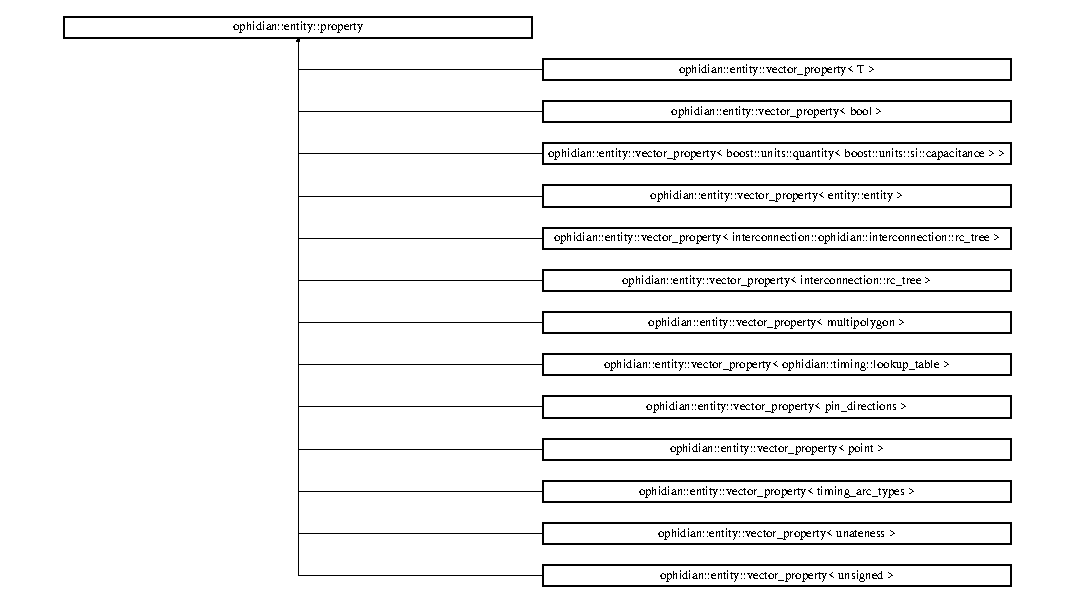
\includegraphics[height=7.656250cm]{classophidian_1_1entity_1_1property}
\end{center}
\end{figure}
\subsection*{Public Member Functions}
\begin{DoxyCompactItemize}
\item 
\hypertarget{classophidian_1_1entity_1_1property_a0fc51c3735e4d44e0460aeca0ffc843f}{virtual \hyperlink{classophidian_1_1entity_1_1property_a0fc51c3735e4d44e0460aeca0ffc843f}{$\sim$property} ()}\label{classophidian_1_1entity_1_1property_a0fc51c3735e4d44e0460aeca0ffc843f}

\begin{DoxyCompactList}\small\item\em Virtual destructor. \end{DoxyCompactList}\item 
virtual void \hyperlink{classophidian_1_1entity_1_1property_a41d49c84d20e3bc9cba0162c9aba6f2b}{destroy} (\hyperlink{classophidian_1_1entity_1_1entity}{entity} \&e, std\-::size\-\_\-t index)=0
\begin{DoxyCompactList}\small\item\em Virtual destroy method. \end{DoxyCompactList}\item 
virtual void \hyperlink{classophidian_1_1entity_1_1property_a25f0188c1d920cbdb55583772b4817ce}{create} (\hyperlink{classophidian_1_1entity_1_1entity}{entity} \&e, std\-::size\-\_\-t index)=0
\begin{DoxyCompactList}\small\item\em Virtual create method. \end{DoxyCompactList}\end{DoxyCompactItemize}


\subsection{Detailed Description}
Describes a property that can be associated to an entity system. 

\subsection{Member Function Documentation}
\hypertarget{classophidian_1_1entity_1_1property_a25f0188c1d920cbdb55583772b4817ce}{\index{ophidian\-::entity\-::property@{ophidian\-::entity\-::property}!create@{create}}
\index{create@{create}!ophidian::entity::property@{ophidian\-::entity\-::property}}
\subsubsection[{create}]{\setlength{\rightskip}{0pt plus 5cm}virtual void ophidian\-::entity\-::property\-::create (
\begin{DoxyParamCaption}
\item[{{\bf entity} \&}]{e, }
\item[{std\-::size\-\_\-t}]{index}
\end{DoxyParamCaption}
)\hspace{0.3cm}{\ttfamily [pure virtual]}}}\label{classophidian_1_1entity_1_1property_a25f0188c1d920cbdb55583772b4817ce}
This method is called when a new entity is created in the system. 
\begin{DoxyParams}{Parameters}
{\em e} & Entity that was created \\
\hline
{\em index} & The index of the created entity \\
\hline
\end{DoxyParams}


Implemented in \hyperlink{classophidian_1_1entity_1_1vector__property_3_01bool_01_4_a3a00eae6f787b0d5cb5b782c931f2774}{ophidian\-::entity\-::vector\-\_\-property$<$ bool $>$}, \hyperlink{classophidian_1_1entity_1_1vector__property_a15ebc0490d8232671cd9111f11351acf}{ophidian\-::entity\-::vector\-\_\-property$<$ T $>$}, \hyperlink{classophidian_1_1entity_1_1vector__property_a15ebc0490d8232671cd9111f11351acf}{ophidian\-::entity\-::vector\-\_\-property$<$ boost\-::optional$<$ std\-::size\-\_\-t $>$ $>$}, \hyperlink{classophidian_1_1entity_1_1vector__property_a15ebc0490d8232671cd9111f11351acf}{ophidian\-::entity\-::vector\-\_\-property$<$ entity\-::entity $>$}, \hyperlink{classophidian_1_1entity_1_1vector__property_a15ebc0490d8232671cd9111f11351acf}{ophidian\-::entity\-::vector\-\_\-property$<$ timing\-\_\-arc\-\_\-types $>$}, \hyperlink{classophidian_1_1entity_1_1vector__property_a15ebc0490d8232671cd9111f11351acf}{ophidian\-::entity\-::vector\-\_\-property$<$ std\-::string $>$}, \hyperlink{classophidian_1_1entity_1_1vector__property_a15ebc0490d8232671cd9111f11351acf}{ophidian\-::entity\-::vector\-\_\-property$<$ unateness $>$}, \hyperlink{classophidian_1_1entity_1_1vector__property_a15ebc0490d8232671cd9111f11351acf}{ophidian\-::entity\-::vector\-\_\-property$<$ boost\-::units\-::quantity$<$ boost\-::units\-::si\-::capacitance $>$ $>$}, \hyperlink{classophidian_1_1entity_1_1vector__property_a15ebc0490d8232671cd9111f11351acf}{ophidian\-::entity\-::vector\-\_\-property$<$ interconnection\-::ophidian\-::interconnection\-::rc\-\_\-tree $>$}, \hyperlink{classophidian_1_1entity_1_1vector__property_a15ebc0490d8232671cd9111f11351acf}{ophidian\-::entity\-::vector\-\_\-property$<$ pin\-\_\-directions $>$}, \hyperlink{classophidian_1_1entity_1_1vector__property_a15ebc0490d8232671cd9111f11351acf}{ophidian\-::entity\-::vector\-\_\-property$<$ unsigned $>$}, \hyperlink{classophidian_1_1entity_1_1vector__property_a15ebc0490d8232671cd9111f11351acf}{ophidian\-::entity\-::vector\-\_\-property$<$ std\-::vector$<$ entity\-::entity $>$ $>$}, \hyperlink{classophidian_1_1entity_1_1vector__property_a15ebc0490d8232671cd9111f11351acf}{ophidian\-::entity\-::vector\-\_\-property$<$ interconnection\-::rc\-\_\-tree $>$}, \hyperlink{classophidian_1_1entity_1_1vector__property_a15ebc0490d8232671cd9111f11351acf}{ophidian\-::entity\-::vector\-\_\-property$<$ point $>$}, \hyperlink{classophidian_1_1entity_1_1vector__property_a15ebc0490d8232671cd9111f11351acf}{ophidian\-::entity\-::vector\-\_\-property$<$ multipolygon $>$}, and \hyperlink{classophidian_1_1entity_1_1vector__property_a15ebc0490d8232671cd9111f11351acf}{ophidian\-::entity\-::vector\-\_\-property$<$ ophidian\-::timing\-::lookup\-\_\-table $>$}.

\hypertarget{classophidian_1_1entity_1_1property_a41d49c84d20e3bc9cba0162c9aba6f2b}{\index{ophidian\-::entity\-::property@{ophidian\-::entity\-::property}!destroy@{destroy}}
\index{destroy@{destroy}!ophidian::entity::property@{ophidian\-::entity\-::property}}
\subsubsection[{destroy}]{\setlength{\rightskip}{0pt plus 5cm}virtual void ophidian\-::entity\-::property\-::destroy (
\begin{DoxyParamCaption}
\item[{{\bf entity} \&}]{e, }
\item[{std\-::size\-\_\-t}]{index}
\end{DoxyParamCaption}
)\hspace{0.3cm}{\ttfamily [pure virtual]}}}\label{classophidian_1_1entity_1_1property_a41d49c84d20e3bc9cba0162c9aba6f2b}
This method is called when an entity in the system is destroyed. 
\begin{DoxyParams}{Parameters}
{\em e} & Entity that was destroyed \\
\hline
{\em index} & The index of the destroyed entity \\
\hline
\end{DoxyParams}


Implemented in \hyperlink{classophidian_1_1entity_1_1vector__property_3_01bool_01_4_a3d61196d880589d68bf68d81c3310643}{ophidian\-::entity\-::vector\-\_\-property$<$ bool $>$}, \hyperlink{classophidian_1_1entity_1_1vector__property_a6b239378e987a33fd05c69bd57158bdc}{ophidian\-::entity\-::vector\-\_\-property$<$ T $>$}, \hyperlink{classophidian_1_1entity_1_1vector__property_a6b239378e987a33fd05c69bd57158bdc}{ophidian\-::entity\-::vector\-\_\-property$<$ boost\-::optional$<$ std\-::size\-\_\-t $>$ $>$}, \hyperlink{classophidian_1_1entity_1_1vector__property_a6b239378e987a33fd05c69bd57158bdc}{ophidian\-::entity\-::vector\-\_\-property$<$ entity\-::entity $>$}, \hyperlink{classophidian_1_1entity_1_1vector__property_a6b239378e987a33fd05c69bd57158bdc}{ophidian\-::entity\-::vector\-\_\-property$<$ timing\-\_\-arc\-\_\-types $>$}, \hyperlink{classophidian_1_1entity_1_1vector__property_a6b239378e987a33fd05c69bd57158bdc}{ophidian\-::entity\-::vector\-\_\-property$<$ std\-::string $>$}, \hyperlink{classophidian_1_1entity_1_1vector__property_a6b239378e987a33fd05c69bd57158bdc}{ophidian\-::entity\-::vector\-\_\-property$<$ unateness $>$}, \hyperlink{classophidian_1_1entity_1_1vector__property_a6b239378e987a33fd05c69bd57158bdc}{ophidian\-::entity\-::vector\-\_\-property$<$ boost\-::units\-::quantity$<$ boost\-::units\-::si\-::capacitance $>$ $>$}, \hyperlink{classophidian_1_1entity_1_1vector__property_a6b239378e987a33fd05c69bd57158bdc}{ophidian\-::entity\-::vector\-\_\-property$<$ interconnection\-::ophidian\-::interconnection\-::rc\-\_\-tree $>$}, \hyperlink{classophidian_1_1entity_1_1vector__property_a6b239378e987a33fd05c69bd57158bdc}{ophidian\-::entity\-::vector\-\_\-property$<$ pin\-\_\-directions $>$}, \hyperlink{classophidian_1_1entity_1_1vector__property_a6b239378e987a33fd05c69bd57158bdc}{ophidian\-::entity\-::vector\-\_\-property$<$ unsigned $>$}, \hyperlink{classophidian_1_1entity_1_1vector__property_a6b239378e987a33fd05c69bd57158bdc}{ophidian\-::entity\-::vector\-\_\-property$<$ std\-::vector$<$ entity\-::entity $>$ $>$}, \hyperlink{classophidian_1_1entity_1_1vector__property_a6b239378e987a33fd05c69bd57158bdc}{ophidian\-::entity\-::vector\-\_\-property$<$ interconnection\-::rc\-\_\-tree $>$}, \hyperlink{classophidian_1_1entity_1_1vector__property_a6b239378e987a33fd05c69bd57158bdc}{ophidian\-::entity\-::vector\-\_\-property$<$ point $>$}, \hyperlink{classophidian_1_1entity_1_1vector__property_a6b239378e987a33fd05c69bd57158bdc}{ophidian\-::entity\-::vector\-\_\-property$<$ multipolygon $>$}, and \hyperlink{classophidian_1_1entity_1_1vector__property_a6b239378e987a33fd05c69bd57158bdc}{ophidian\-::entity\-::vector\-\_\-property$<$ ophidian\-::timing\-::lookup\-\_\-table $>$}.



The documentation for this class was generated from the following file\-:\begin{DoxyCompactItemize}
\item 
/home/renan/workspace/openeda/src/entity/property.\-h\end{DoxyCompactItemize}

\hypertarget{classophidian_1_1interconnection_1_1rc__tree}{\section{ophidian\-:\-:interconnection\-:\-:rc\-\_\-tree Class Reference}
\label{classophidian_1_1interconnection_1_1rc__tree}\index{ophidian\-::interconnection\-::rc\-\_\-tree@{ophidian\-::interconnection\-::rc\-\_\-tree}}
}
\subsection*{Public Types}
\begin{DoxyCompactItemize}
\item 
\hypertarget{classophidian_1_1interconnection_1_1rc__tree_a3150567e8388e615a01021accf9544a2}{using {\bfseries graph\-\_\-t} = lemon\-::\-List\-Graph}\label{classophidian_1_1interconnection_1_1rc__tree_a3150567e8388e615a01021accf9544a2}

\item 
\hypertarget{classophidian_1_1interconnection_1_1rc__tree_a924f23b7ccb8c4fcc9a0782efd0fd96b}{using {\bfseries capacitor\-\_\-id} = lemon\-::\-List\-Graph\-::\-Node}\label{classophidian_1_1interconnection_1_1rc__tree_a924f23b7ccb8c4fcc9a0782efd0fd96b}

\item 
\hypertarget{classophidian_1_1interconnection_1_1rc__tree_a6f88448d10474e21d5c341f598154b0a}{using {\bfseries resistor\-\_\-id} = lemon\-::\-List\-Graph\-::\-Edge}\label{classophidian_1_1interconnection_1_1rc__tree_a6f88448d10474e21d5c341f598154b0a}

\item 
\hypertarget{classophidian_1_1interconnection_1_1rc__tree_abd7eab88b02ff1c1f70e2f6f6fe495b7}{using {\bfseries resistor\-\_\-it} = lemon\-::\-List\-Graph\-::\-Inc\-Edge\-It}\label{classophidian_1_1interconnection_1_1rc__tree_abd7eab88b02ff1c1f70e2f6f6fe495b7}

\end{DoxyCompactItemize}
\subsection*{Public Member Functions}
\begin{DoxyCompactItemize}
\item 
\hypertarget{classophidian_1_1interconnection_1_1rc__tree_a0df0ca1855bfac8e8b762d1421de7017}{{\bfseries rc\-\_\-tree} (const \hyperlink{classophidian_1_1interconnection_1_1rc__tree}{rc\-\_\-tree} \&other)}\label{classophidian_1_1interconnection_1_1rc__tree_a0df0ca1855bfac8e8b762d1421de7017}

\item 
\hypertarget{classophidian_1_1interconnection_1_1rc__tree_aa7c55c652bed438a4aee8f677b23106d}{\hyperlink{classophidian_1_1interconnection_1_1rc__tree}{rc\-\_\-tree} \& {\bfseries operator=} (const \hyperlink{classophidian_1_1interconnection_1_1rc__tree}{rc\-\_\-tree} \&other)}\label{classophidian_1_1interconnection_1_1rc__tree_aa7c55c652bed438a4aee8f677b23106d}

\item 
\hypertarget{classophidian_1_1interconnection_1_1rc__tree_a592637445f8764ca6749d6baf04ca8ba}{quantity$<$ si\-::capacitance $>$ {\bfseries lumped} () const }\label{classophidian_1_1interconnection_1_1rc__tree_a592637445f8764ca6749d6baf04ca8ba}

\item 
\hypertarget{classophidian_1_1interconnection_1_1rc__tree_a800437d718c8a08ddc406aad005fe305}{capacitor\-\_\-id {\bfseries capacitor\-\_\-insert} (std\-::string name)}\label{classophidian_1_1interconnection_1_1rc__tree_a800437d718c8a08ddc406aad005fe305}

\item 
\hypertarget{classophidian_1_1interconnection_1_1rc__tree_a89db718c78d9ab237e3bcc461b10c350}{std\-::string {\bfseries capacitor\-\_\-name} (capacitor\-\_\-id u) const }\label{classophidian_1_1interconnection_1_1rc__tree_a89db718c78d9ab237e3bcc461b10c350}

\item 
\hypertarget{classophidian_1_1interconnection_1_1rc__tree_a29601551ac7d8d622ef12dd72a373dab}{std\-::size\-\_\-t {\bfseries capacitor\-\_\-count} () const }\label{classophidian_1_1interconnection_1_1rc__tree_a29601551ac7d8d622ef12dd72a373dab}

\item 
\hypertarget{classophidian_1_1interconnection_1_1rc__tree_a9d9fa55505a49e5adc7847f485711987}{resistor\-\_\-id {\bfseries resistor\-\_\-insert} (capacitor\-\_\-id u, capacitor\-\_\-id v, quantity$<$ si\-::resistance $>$ res)}\label{classophidian_1_1interconnection_1_1rc__tree_a9d9fa55505a49e5adc7847f485711987}

\item 
\hypertarget{classophidian_1_1interconnection_1_1rc__tree_a4db2106df9ff03422a9efa996d9dabfe}{void {\bfseries capacitance} (capacitor\-\_\-id u, quantity$<$ si\-::capacitance $>$ cap)}\label{classophidian_1_1interconnection_1_1rc__tree_a4db2106df9ff03422a9efa996d9dabfe}

\item 
\hypertarget{classophidian_1_1interconnection_1_1rc__tree_a27d52641b61ecb5722f5c9f7e183f674}{capacitor\-\_\-id {\bfseries capacitor\-\_\-by\-\_\-name} (std\-::string name) const }\label{classophidian_1_1interconnection_1_1rc__tree_a27d52641b61ecb5722f5c9f7e183f674}

\item 
\hypertarget{classophidian_1_1interconnection_1_1rc__tree_a4b3aad5a72af43566289e6de214ace50}{quantity$<$ si\-::capacitance $>$ {\bfseries capacitance} (capacitor\-\_\-id u) const }\label{classophidian_1_1interconnection_1_1rc__tree_a4b3aad5a72af43566289e6de214ace50}

\item 
\hypertarget{classophidian_1_1interconnection_1_1rc__tree_a15276013af4bb7283f62656531ffecfb}{quantity$<$ si\-::resistance $>$ {\bfseries resistance} (resistor\-\_\-id uv) const }\label{classophidian_1_1interconnection_1_1rc__tree_a15276013af4bb7283f62656531ffecfb}

\item 
\hypertarget{classophidian_1_1interconnection_1_1rc__tree_a1c296a5067234cb99ce6a8ca1f085c75}{resistor\-\_\-it {\bfseries capacitor\-\_\-resistors} (capacitor\-\_\-id u) const }\label{classophidian_1_1interconnection_1_1rc__tree_a1c296a5067234cb99ce6a8ca1f085c75}

\item 
\hypertarget{classophidian_1_1interconnection_1_1rc__tree_a612ffed536ea1fbaf6e7574f4e0a6531}{capacitor\-\_\-id {\bfseries other\-\_\-capacitor} (resistor\-\_\-id res, capacitor\-\_\-id cap) const }\label{classophidian_1_1interconnection_1_1rc__tree_a612ffed536ea1fbaf6e7574f4e0a6531}

\item 
\hypertarget{classophidian_1_1interconnection_1_1rc__tree_a52102a355b292bca74f6494663c477e8}{const graph\-\_\-t \& {\bfseries graph} () const }\label{classophidian_1_1interconnection_1_1rc__tree_a52102a355b292bca74f6494663c477e8}

\end{DoxyCompactItemize}
\subsection*{Static Public Member Functions}
\begin{DoxyCompactItemize}
\item 
\hypertarget{classophidian_1_1interconnection_1_1rc__tree_aa4187806724136382911946a0112ccf4}{static resistor\-\_\-it {\bfseries invalid} ()}\label{classophidian_1_1interconnection_1_1rc__tree_aa4187806724136382911946a0112ccf4}

\end{DoxyCompactItemize}


The documentation for this class was generated from the following files\-:\begin{DoxyCompactItemize}
\item 
/home/renan/workspace/openeda/src/interconnection/rc\-\_\-tree.\-h\item 
/home/renan/workspace/openeda/src/interconnection/rc\-\_\-tree.\-cpp\end{DoxyCompactItemize}

\hypertarget{classophidian_1_1floorplan_1_1rows}{\section{ophidian\-:\-:floorplan\-:\-:rows Class Reference}
\label{classophidian_1_1floorplan_1_1rows}\index{ophidian\-::floorplan\-::rows@{ophidian\-::floorplan\-::rows}}
}


Rows class.  




{\ttfamily \#include $<$rows.\-h$>$}

\subsection*{Public Member Functions}
\begin{DoxyCompactItemize}
\item 
\hyperlink{classophidian_1_1floorplan_1_1rows_a615ba2d1e4ca91c9faf91e9f2d53efed}{rows} (\hyperlink{classophidian_1_1entity_1_1system}{entity\-::system} \&system)
\begin{DoxyCompactList}\small\item\em Constructor. \end{DoxyCompactList}\item 
\hyperlink{classophidian_1_1entity_1_1entity}{entity\-::entity} \hyperlink{classophidian_1_1floorplan_1_1rows_ad752fabe326be190ca1db1c6f3041a05}{site} (\hyperlink{classophidian_1_1entity_1_1entity}{entity\-::entity} row) const 
\begin{DoxyCompactList}\small\item\em Site getter. \end{DoxyCompactList}\item 
unsigned \hyperlink{classophidian_1_1floorplan_1_1rows_a4f502b7792681191ab717db70370622e}{number\-\_\-of\-\_\-sites} (\hyperlink{classophidian_1_1entity_1_1entity}{entity\-::entity} row) const 
\begin{DoxyCompactList}\small\item\em Number of sites getter. \end{DoxyCompactList}\item 
point \hyperlink{classophidian_1_1floorplan_1_1rows_a7dd1c9c3743ca06933fa6fc120e65d57}{origin} (\hyperlink{classophidian_1_1entity_1_1entity}{entity\-::entity} row) const 
\begin{DoxyCompactList}\small\item\em Row origin getter. \end{DoxyCompactList}\item 
std\-::pair$<$ std\-::vector\\*
$<$ \hyperlink{classophidian_1_1entity_1_1entity}{entity\-::entity} $>$\\*
\-::const\-\_\-iterator, std\-::vector\\*
$<$ \hyperlink{classophidian_1_1entity_1_1entity}{entity\-::entity} $>$\\*
\-::const\-\_\-iterator $>$ \hyperlink{classophidian_1_1floorplan_1_1rows_a259f8f0511ad0e1c139b97a418aca957}{sites} () const 
\begin{DoxyCompactList}\small\item\em Sites iterator getter. \end{DoxyCompactList}\item 
std\-::pair$<$ std\-::vector\\*
$<$ unsigned $>$\-::const\-\_\-iterator, \\*
std\-::vector$<$ unsigned $>$\\*
\-::const\-\_\-iterator $>$ \hyperlink{classophidian_1_1floorplan_1_1rows_ad9da40317e6b4eaada1893b925bca1f4}{number\-\_\-of\-\_\-sites} () const 
\begin{DoxyCompactList}\small\item\em Number of sites iterator getter. \end{DoxyCompactList}\item 
std\-::pair$<$ std\-::vector$<$ point $>$\\*
\-::const\-\_\-iterator, std\-::vector\\*
$<$ point $>$\-::const\-\_\-iterator $>$ \hyperlink{classophidian_1_1floorplan_1_1rows_a37a388de47fe14525780086d17e3bcfb}{origins} () const 
\begin{DoxyCompactList}\small\item\em Origins iterator getter. \end{DoxyCompactList}\item 
void \hyperlink{classophidian_1_1floorplan_1_1rows_ac4ea14b0ce48d27aca9b8522bb501b14}{site} (\hyperlink{classophidian_1_1entity_1_1entity}{entity\-::entity} row, \hyperlink{classophidian_1_1entity_1_1entity}{entity\-::entity} site)
\begin{DoxyCompactList}\small\item\em Site setter. \end{DoxyCompactList}\item 
void \hyperlink{classophidian_1_1floorplan_1_1rows_a590b0a0b337edaa5d52d2ad272cd6736}{number\-\_\-of\-\_\-sites} (\hyperlink{classophidian_1_1entity_1_1entity}{entity\-::entity} row, unsigned number\-\_\-of\-\_\-sites)
\begin{DoxyCompactList}\small\item\em Number of sites setter. \end{DoxyCompactList}\item 
void \hyperlink{classophidian_1_1floorplan_1_1rows_a497e85a03604c2c3fb1f44fdbeafa260}{origin} (\hyperlink{classophidian_1_1entity_1_1entity}{entity\-::entity} row, point origin)
\begin{DoxyCompactList}\small\item\em Origin setter. \end{DoxyCompactList}\end{DoxyCompactItemize}


\subsection{Detailed Description}
This class describes the properties of rows initialized by the floorplan module. 

\subsection{Constructor \& Destructor Documentation}
\hypertarget{classophidian_1_1floorplan_1_1rows_a615ba2d1e4ca91c9faf91e9f2d53efed}{\index{ophidian\-::floorplan\-::rows@{ophidian\-::floorplan\-::rows}!rows@{rows}}
\index{rows@{rows}!ophidian::floorplan::rows@{ophidian\-::floorplan\-::rows}}
\subsubsection[{rows}]{\setlength{\rightskip}{0pt plus 5cm}ophidian\-::floorplan\-::rows\-::rows (
\begin{DoxyParamCaption}
\item[{{\bf entity\-::system} \&}]{system}
\end{DoxyParamCaption}
)}}\label{classophidian_1_1floorplan_1_1rows_a615ba2d1e4ca91c9faf91e9f2d53efed}
Rows object constructor. Register the rows properties to the rows system. 
\begin{DoxyParams}{Parameters}
{\em system} & Rows entity system. \\
\hline
\end{DoxyParams}


\subsection{Member Function Documentation}
\hypertarget{classophidian_1_1floorplan_1_1rows_a4f502b7792681191ab717db70370622e}{\index{ophidian\-::floorplan\-::rows@{ophidian\-::floorplan\-::rows}!number\-\_\-of\-\_\-sites@{number\-\_\-of\-\_\-sites}}
\index{number\-\_\-of\-\_\-sites@{number\-\_\-of\-\_\-sites}!ophidian::floorplan::rows@{ophidian\-::floorplan\-::rows}}
\subsubsection[{number\-\_\-of\-\_\-sites}]{\setlength{\rightskip}{0pt plus 5cm}unsigned ophidian\-::floorplan\-::rows\-::number\-\_\-of\-\_\-sites (
\begin{DoxyParamCaption}
\item[{{\bf entity\-::entity}}]{row}
\end{DoxyParamCaption}
) const\hspace{0.3cm}{\ttfamily [inline]}}}\label{classophidian_1_1floorplan_1_1rows_a4f502b7792681191ab717db70370622e}
Returns the number of sites in a row. 
\begin{DoxyParams}{Parameters}
{\em row} & Row entity to get the number of sites. \\
\hline
\end{DoxyParams}
\begin{DoxyReturn}{Returns}
Number of sites of the row. 
\end{DoxyReturn}
\hypertarget{classophidian_1_1floorplan_1_1rows_ad9da40317e6b4eaada1893b925bca1f4}{\index{ophidian\-::floorplan\-::rows@{ophidian\-::floorplan\-::rows}!number\-\_\-of\-\_\-sites@{number\-\_\-of\-\_\-sites}}
\index{number\-\_\-of\-\_\-sites@{number\-\_\-of\-\_\-sites}!ophidian::floorplan::rows@{ophidian\-::floorplan\-::rows}}
\subsubsection[{number\-\_\-of\-\_\-sites}]{\setlength{\rightskip}{0pt plus 5cm}std\-::pair$<$ std\-::vector$<$unsigned$>$\-::const\-\_\-iterator, std\-::vector$<$unsigned$>$\-::const\-\_\-iterator $>$ ophidian\-::floorplan\-::rows\-::number\-\_\-of\-\_\-sites (
\begin{DoxyParamCaption}
{}
\end{DoxyParamCaption}
) const\hspace{0.3cm}{\ttfamily [inline]}}}\label{classophidian_1_1floorplan_1_1rows_ad9da40317e6b4eaada1893b925bca1f4}
Returns the begin and end iterator of the row number of sites property. \begin{DoxyReturn}{Returns}
Pair with constant iterators pointing the the beginning and end of the number of sites property. 
\end{DoxyReturn}
\hypertarget{classophidian_1_1floorplan_1_1rows_a590b0a0b337edaa5d52d2ad272cd6736}{\index{ophidian\-::floorplan\-::rows@{ophidian\-::floorplan\-::rows}!number\-\_\-of\-\_\-sites@{number\-\_\-of\-\_\-sites}}
\index{number\-\_\-of\-\_\-sites@{number\-\_\-of\-\_\-sites}!ophidian::floorplan::rows@{ophidian\-::floorplan\-::rows}}
\subsubsection[{number\-\_\-of\-\_\-sites}]{\setlength{\rightskip}{0pt plus 5cm}void ophidian\-::floorplan\-::rows\-::number\-\_\-of\-\_\-sites (
\begin{DoxyParamCaption}
\item[{{\bf entity\-::entity}}]{row, }
\item[{unsigned}]{number\-\_\-of\-\_\-sites}
\end{DoxyParamCaption}
)}}\label{classophidian_1_1floorplan_1_1rows_a590b0a0b337edaa5d52d2ad272cd6736}
Sets the number of sites of a row. 
\begin{DoxyParams}{Parameters}
{\em row} & Row entity to set the number of sites. \\
\hline
{\em number\-\_\-of\-\_\-sites} & Number of sites to set. \\
\hline
\end{DoxyParams}
\hypertarget{classophidian_1_1floorplan_1_1rows_a7dd1c9c3743ca06933fa6fc120e65d57}{\index{ophidian\-::floorplan\-::rows@{ophidian\-::floorplan\-::rows}!origin@{origin}}
\index{origin@{origin}!ophidian::floorplan::rows@{ophidian\-::floorplan\-::rows}}
\subsubsection[{origin}]{\setlength{\rightskip}{0pt plus 5cm}point ophidian\-::floorplan\-::rows\-::origin (
\begin{DoxyParamCaption}
\item[{{\bf entity\-::entity}}]{row}
\end{DoxyParamCaption}
) const\hspace{0.3cm}{\ttfamily [inline]}}}\label{classophidian_1_1floorplan_1_1rows_a7dd1c9c3743ca06933fa6fc120e65d57}
Returns the origin of a row. 
\begin{DoxyParams}{Parameters}
{\em row} & Row entity to get the origin. \\
\hline
\end{DoxyParams}
\begin{DoxyReturn}{Returns}
Point describing the row origin. 
\end{DoxyReturn}
\hypertarget{classophidian_1_1floorplan_1_1rows_a497e85a03604c2c3fb1f44fdbeafa260}{\index{ophidian\-::floorplan\-::rows@{ophidian\-::floorplan\-::rows}!origin@{origin}}
\index{origin@{origin}!ophidian::floorplan::rows@{ophidian\-::floorplan\-::rows}}
\subsubsection[{origin}]{\setlength{\rightskip}{0pt plus 5cm}void ophidian\-::floorplan\-::rows\-::origin (
\begin{DoxyParamCaption}
\item[{{\bf entity\-::entity}}]{row, }
\item[{rows\-::point}]{origin}
\end{DoxyParamCaption}
)}}\label{classophidian_1_1floorplan_1_1rows_a497e85a03604c2c3fb1f44fdbeafa260}
Sets the origin of a row. 
\begin{DoxyParams}{Parameters}
{\em row} & Row entity to set the origin. \\
\hline
{\em origin} & Origin to set. \\
\hline
\end{DoxyParams}
\hypertarget{classophidian_1_1floorplan_1_1rows_a37a388de47fe14525780086d17e3bcfb}{\index{ophidian\-::floorplan\-::rows@{ophidian\-::floorplan\-::rows}!origins@{origins}}
\index{origins@{origins}!ophidian::floorplan::rows@{ophidian\-::floorplan\-::rows}}
\subsubsection[{origins}]{\setlength{\rightskip}{0pt plus 5cm}std\-::pair$<$ std\-::vector$<$point$>$\-::const\-\_\-iterator, std\-::vector$<$point$>$\-::const\-\_\-iterator $>$ ophidian\-::floorplan\-::rows\-::origins (
\begin{DoxyParamCaption}
{}
\end{DoxyParamCaption}
) const\hspace{0.3cm}{\ttfamily [inline]}}}\label{classophidian_1_1floorplan_1_1rows_a37a388de47fe14525780086d17e3bcfb}
Returns the begin and end iterator of the row origins property. \begin{DoxyReturn}{Returns}
Pair with constant iterators pointing the the beginning and end of the origins property. 
\end{DoxyReturn}
\hypertarget{classophidian_1_1floorplan_1_1rows_ad752fabe326be190ca1db1c6f3041a05}{\index{ophidian\-::floorplan\-::rows@{ophidian\-::floorplan\-::rows}!site@{site}}
\index{site@{site}!ophidian::floorplan::rows@{ophidian\-::floorplan\-::rows}}
\subsubsection[{site}]{\setlength{\rightskip}{0pt plus 5cm}{\bf entity\-::entity} ophidian\-::floorplan\-::rows\-::site (
\begin{DoxyParamCaption}
\item[{{\bf entity\-::entity}}]{row}
\end{DoxyParamCaption}
) const\hspace{0.3cm}{\ttfamily [inline]}}}\label{classophidian_1_1floorplan_1_1rows_ad752fabe326be190ca1db1c6f3041a05}
Returns the site composing a row. 
\begin{DoxyParams}{Parameters}
{\em row} & Row entity to get the site. \\
\hline
\end{DoxyParams}
\begin{DoxyReturn}{Returns}
Site entity. 
\end{DoxyReturn}
\hypertarget{classophidian_1_1floorplan_1_1rows_ac4ea14b0ce48d27aca9b8522bb501b14}{\index{ophidian\-::floorplan\-::rows@{ophidian\-::floorplan\-::rows}!site@{site}}
\index{site@{site}!ophidian::floorplan::rows@{ophidian\-::floorplan\-::rows}}
\subsubsection[{site}]{\setlength{\rightskip}{0pt plus 5cm}void ophidian\-::floorplan\-::rows\-::site (
\begin{DoxyParamCaption}
\item[{{\bf entity\-::entity}}]{row, }
\item[{{\bf entity\-::entity}}]{site}
\end{DoxyParamCaption}
)}}\label{classophidian_1_1floorplan_1_1rows_ac4ea14b0ce48d27aca9b8522bb501b14}
Sets the site of a row. 
\begin{DoxyParams}{Parameters}
{\em row} & Row entity to set the site. \\
\hline
{\em site} & Site entity to set. \\
\hline
\end{DoxyParams}
\hypertarget{classophidian_1_1floorplan_1_1rows_a259f8f0511ad0e1c139b97a418aca957}{\index{ophidian\-::floorplan\-::rows@{ophidian\-::floorplan\-::rows}!sites@{sites}}
\index{sites@{sites}!ophidian::floorplan::rows@{ophidian\-::floorplan\-::rows}}
\subsubsection[{sites}]{\setlength{\rightskip}{0pt plus 5cm}std\-::pair$<$ std\-::vector$<${\bf entity\-::entity}$>$\-::const\-\_\-iterator, std\-::vector$<${\bf entity\-::entity}$>$\-::const\-\_\-iterator $>$ ophidian\-::floorplan\-::rows\-::sites (
\begin{DoxyParamCaption}
{}
\end{DoxyParamCaption}
) const\hspace{0.3cm}{\ttfamily [inline]}}}\label{classophidian_1_1floorplan_1_1rows_a259f8f0511ad0e1c139b97a418aca957}
Returns the begin and end iterator of the row sites property. \begin{DoxyReturn}{Returns}
Pair with constant iterators pointing the the beginning and end of the sites property. 
\end{DoxyReturn}


The documentation for this class was generated from the following files\-:\begin{DoxyCompactItemize}
\item 
/home/csguth/workspace/openeda/src/floorplan/rows.\-h\item 
/home/csguth/workspace/openeda/src/floorplan/rows.\-cpp\end{DoxyCompactItemize}

\hypertarget{classophidian_1_1timingdriven__placement_1_1flute__rc__tree__rtree_1_1rtree__node__comparator}{\section{ophidian\-:\-:timingdriven\-\_\-placement\-:\-:flute\-\_\-rc\-\_\-tree\-\_\-rtree\-:\-:rtree\-\_\-node\-\_\-comparator Class Reference}
\label{classophidian_1_1timingdriven__placement_1_1flute__rc__tree__rtree_1_1rtree__node__comparator}\index{ophidian\-::timingdriven\-\_\-placement\-::flute\-\_\-rc\-\_\-tree\-\_\-rtree\-::rtree\-\_\-node\-\_\-comparator@{ophidian\-::timingdriven\-\_\-placement\-::flute\-\_\-rc\-\_\-tree\-\_\-rtree\-::rtree\-\_\-node\-\_\-comparator}}
}
\subsection*{Public Member Functions}
\begin{DoxyCompactItemize}
\item 
\hypertarget{classophidian_1_1timingdriven__placement_1_1flute__rc__tree__rtree_1_1rtree__node__comparator_a1fb8b85507617390a63ae8be20a4c706}{bool {\bfseries operator()} (const rtree\-\_\-node \&node1, const rtree\-\_\-node \&node2) const }\label{classophidian_1_1timingdriven__placement_1_1flute__rc__tree__rtree_1_1rtree__node__comparator_a1fb8b85507617390a63ae8be20a4c706}

\end{DoxyCompactItemize}


The documentation for this class was generated from the following file\-:\begin{DoxyCompactItemize}
\item 
/home/csguth/workspace/openeda/src/timing-\/driven\-\_\-placement/flute\-\_\-rc\-\_\-tree\-\_\-estimation.\-cpp\end{DoxyCompactItemize}

\hypertarget{classophidian_1_1timing_1_1simple__design__constraint}{\section{ophidian\-:\-:timing\-:\-:simple\-\_\-design\-\_\-constraint Class Reference}
\label{classophidian_1_1timing_1_1simple__design__constraint}\index{ophidian\-::timing\-::simple\-\_\-design\-\_\-constraint@{ophidian\-::timing\-::simple\-\_\-design\-\_\-constraint}}
}
\subsection*{Public Member Functions}
\begin{DoxyCompactItemize}
\item 
\hypertarget{classophidian_1_1timing_1_1simple__design__constraint_addeba923b2f0e7ee29585c2d0800a06d}{const \hyperlink{structophidian_1_1timing_1_1design__constraints}{design\-\_\-constraints} \& {\bfseries dc} () const }\label{classophidian_1_1timing_1_1simple__design__constraint_addeba923b2f0e7ee29585c2d0800a06d}

\end{DoxyCompactItemize}


The documentation for this class was generated from the following files\-:\begin{DoxyCompactItemize}
\item 
/home/csguth/workspace/openeda/src/timing/simple\-\_\-design\-\_\-constraint.\-h\item 
/home/csguth/workspace/openeda/src/timing/simple\-\_\-design\-\_\-constraint.\-cpp\end{DoxyCompactItemize}

\hypertarget{classophidian_1_1floorplan_1_1sites}{\section{ophidian\-:\-:floorplan\-:\-:sites Class Reference}
\label{classophidian_1_1floorplan_1_1sites}\index{ophidian\-::floorplan\-::sites@{ophidian\-::floorplan\-::sites}}
}


Sites class.  




{\ttfamily \#include $<$sites.\-h$>$}

\subsection*{Public Member Functions}
\begin{DoxyCompactItemize}
\item 
\hyperlink{classophidian_1_1floorplan_1_1sites_a448e8d956831330bad88f3bc41ad3897}{sites} (\hyperlink{classophidian_1_1entity_1_1system}{entity\-::system} \&system)
\begin{DoxyCompactList}\small\item\em Constructor. \end{DoxyCompactList}\item 
std\-::string \hyperlink{classophidian_1_1floorplan_1_1sites_aedaadf66a689a9542f3c33da9f76cfd4}{name} (\hyperlink{classophidian_1_1entity_1_1entity}{entity\-::entity} site) const 
\begin{DoxyCompactList}\small\item\em Name getter. \end{DoxyCompactList}\item 
point \hyperlink{classophidian_1_1floorplan_1_1sites_addce4102309e4f3f07e9869ced4bfbc6}{dimensions} (\hyperlink{classophidian_1_1entity_1_1entity}{entity\-::entity} site) const 
\begin{DoxyCompactList}\small\item\em Dimensions getter. \end{DoxyCompactList}\item 
std\-::pair$<$ std\-::vector\\*
$<$ std\-::string $>$\\*
\-::const\-\_\-iterator, std\-::vector\\*
$<$ std\-::string $>$\\*
\-::const\-\_\-iterator $>$ \hyperlink{classophidian_1_1floorplan_1_1sites_abcd874e49de890637581e8b192274b5e}{names} () const 
\begin{DoxyCompactList}\small\item\em Name iterator getter. \end{DoxyCompactList}\item 
std\-::pair$<$ std\-::vector$<$ point $>$\\*
\-::const\-\_\-iterator, std\-::vector\\*
$<$ point $>$\-::const\-\_\-iterator $>$ \hyperlink{classophidian_1_1floorplan_1_1sites_a2cdf9c4052e6ffe35f55e258e18686ce}{dimensions} () const 
\begin{DoxyCompactList}\small\item\em Dimensions iterator getter. \end{DoxyCompactList}\item 
void \hyperlink{classophidian_1_1floorplan_1_1sites_a13693fdb90abc0521bd7c2ef73ef97b7}{name} (\hyperlink{classophidian_1_1entity_1_1entity}{entity\-::entity} site, std\-::string name)
\begin{DoxyCompactList}\small\item\em Name setter. \end{DoxyCompactList}\item 
void \hyperlink{classophidian_1_1floorplan_1_1sites_a48fe05718d1b079ab2da16c5a4290e2c}{dimensions} (\hyperlink{classophidian_1_1entity_1_1entity}{entity\-::entity} site, point dimensions)
\begin{DoxyCompactList}\small\item\em Dimensions setter. \end{DoxyCompactList}\end{DoxyCompactItemize}


\subsection{Detailed Description}
This class describes the properties of sites initialized by the floorplan module. 

\subsection{Constructor \& Destructor Documentation}
\hypertarget{classophidian_1_1floorplan_1_1sites_a448e8d956831330bad88f3bc41ad3897}{\index{ophidian\-::floorplan\-::sites@{ophidian\-::floorplan\-::sites}!sites@{sites}}
\index{sites@{sites}!ophidian::floorplan::sites@{ophidian\-::floorplan\-::sites}}
\subsubsection[{sites}]{\setlength{\rightskip}{0pt plus 5cm}ophidian\-::floorplan\-::sites\-::sites (
\begin{DoxyParamCaption}
\item[{{\bf entity\-::system} \&}]{system}
\end{DoxyParamCaption}
)}}\label{classophidian_1_1floorplan_1_1sites_a448e8d956831330bad88f3bc41ad3897}
Sites object constructor. Register the sites properties to the sites system. 
\begin{DoxyParams}{Parameters}
{\em system} & Sites entity system. \\
\hline
\end{DoxyParams}


\subsection{Member Function Documentation}
\hypertarget{classophidian_1_1floorplan_1_1sites_addce4102309e4f3f07e9869ced4bfbc6}{\index{ophidian\-::floorplan\-::sites@{ophidian\-::floorplan\-::sites}!dimensions@{dimensions}}
\index{dimensions@{dimensions}!ophidian::floorplan::sites@{ophidian\-::floorplan\-::sites}}
\subsubsection[{dimensions}]{\setlength{\rightskip}{0pt plus 5cm}point ophidian\-::floorplan\-::sites\-::dimensions (
\begin{DoxyParamCaption}
\item[{{\bf entity\-::entity}}]{site}
\end{DoxyParamCaption}
) const\hspace{0.3cm}{\ttfamily [inline]}}}\label{classophidian_1_1floorplan_1_1sites_addce4102309e4f3f07e9869ced4bfbc6}
Returns the dimensions of a site. 
\begin{DoxyParams}{Parameters}
{\em site} & Site entity to get the dimensions. \\
\hline
\end{DoxyParams}
\begin{DoxyReturn}{Returns}
Point describing the site dimensions. 
\end{DoxyReturn}
\hypertarget{classophidian_1_1floorplan_1_1sites_a2cdf9c4052e6ffe35f55e258e18686ce}{\index{ophidian\-::floorplan\-::sites@{ophidian\-::floorplan\-::sites}!dimensions@{dimensions}}
\index{dimensions@{dimensions}!ophidian::floorplan::sites@{ophidian\-::floorplan\-::sites}}
\subsubsection[{dimensions}]{\setlength{\rightskip}{0pt plus 5cm}std\-::pair$<$ std\-::vector$<$point$>$\-::const\-\_\-iterator, std\-::vector$<$point$>$\-::const\-\_\-iterator $>$ ophidian\-::floorplan\-::sites\-::dimensions (
\begin{DoxyParamCaption}
{}
\end{DoxyParamCaption}
) const\hspace{0.3cm}{\ttfamily [inline]}}}\label{classophidian_1_1floorplan_1_1sites_a2cdf9c4052e6ffe35f55e258e18686ce}
Returns the begin and end iterator of the site dimensions property. \begin{DoxyReturn}{Returns}
Pair with constant iterators pointing the the beginning and end of the dimensions property. 
\end{DoxyReturn}
\hypertarget{classophidian_1_1floorplan_1_1sites_a48fe05718d1b079ab2da16c5a4290e2c}{\index{ophidian\-::floorplan\-::sites@{ophidian\-::floorplan\-::sites}!dimensions@{dimensions}}
\index{dimensions@{dimensions}!ophidian::floorplan::sites@{ophidian\-::floorplan\-::sites}}
\subsubsection[{dimensions}]{\setlength{\rightskip}{0pt plus 5cm}void ophidian\-::floorplan\-::sites\-::dimensions (
\begin{DoxyParamCaption}
\item[{{\bf entity\-::entity}}]{site, }
\item[{sites\-::point}]{dimensions}
\end{DoxyParamCaption}
)}}\label{classophidian_1_1floorplan_1_1sites_a48fe05718d1b079ab2da16c5a4290e2c}
Sets the dimensions of a site. 
\begin{DoxyParams}{Parameters}
{\em site} & Site entity to set the dimensions. \\
\hline
{\em name} & Desired dimensions to set. \\
\hline
\end{DoxyParams}
\hypertarget{classophidian_1_1floorplan_1_1sites_aedaadf66a689a9542f3c33da9f76cfd4}{\index{ophidian\-::floorplan\-::sites@{ophidian\-::floorplan\-::sites}!name@{name}}
\index{name@{name}!ophidian::floorplan::sites@{ophidian\-::floorplan\-::sites}}
\subsubsection[{name}]{\setlength{\rightskip}{0pt plus 5cm}std\-::string ophidian\-::floorplan\-::sites\-::name (
\begin{DoxyParamCaption}
\item[{{\bf entity\-::entity}}]{site}
\end{DoxyParamCaption}
) const\hspace{0.3cm}{\ttfamily [inline]}}}\label{classophidian_1_1floorplan_1_1sites_aedaadf66a689a9542f3c33da9f76cfd4}
Returns the name of a site. 
\begin{DoxyParams}{Parameters}
{\em site} & Site entity to get the name. \\
\hline
\end{DoxyParams}
\begin{DoxyReturn}{Returns}
Site name. 
\end{DoxyReturn}
\hypertarget{classophidian_1_1floorplan_1_1sites_a13693fdb90abc0521bd7c2ef73ef97b7}{\index{ophidian\-::floorplan\-::sites@{ophidian\-::floorplan\-::sites}!name@{name}}
\index{name@{name}!ophidian::floorplan::sites@{ophidian\-::floorplan\-::sites}}
\subsubsection[{name}]{\setlength{\rightskip}{0pt plus 5cm}void ophidian\-::floorplan\-::sites\-::name (
\begin{DoxyParamCaption}
\item[{{\bf entity\-::entity}}]{site, }
\item[{std\-::string}]{name}
\end{DoxyParamCaption}
)}}\label{classophidian_1_1floorplan_1_1sites_a13693fdb90abc0521bd7c2ef73ef97b7}
Sets the name of a site. 
\begin{DoxyParams}{Parameters}
{\em site} & Site entity to set the name. \\
\hline
{\em name} & Desired name to set. \\
\hline
\end{DoxyParams}
\hypertarget{classophidian_1_1floorplan_1_1sites_abcd874e49de890637581e8b192274b5e}{\index{ophidian\-::floorplan\-::sites@{ophidian\-::floorplan\-::sites}!names@{names}}
\index{names@{names}!ophidian::floorplan::sites@{ophidian\-::floorplan\-::sites}}
\subsubsection[{names}]{\setlength{\rightskip}{0pt plus 5cm}std\-::pair$<$ std\-::vector$<$std\-::string$>$\-::const\-\_\-iterator, std\-::vector$<$std\-::string$>$\-::const\-\_\-iterator $>$ ophidian\-::floorplan\-::sites\-::names (
\begin{DoxyParamCaption}
{}
\end{DoxyParamCaption}
) const\hspace{0.3cm}{\ttfamily [inline]}}}\label{classophidian_1_1floorplan_1_1sites_abcd874e49de890637581e8b192274b5e}
Returns the begin and end iterator of the site names property. \begin{DoxyReturn}{Returns}
Pair with constant iterators pointing the the beginning and end of the names property. 
\end{DoxyReturn}


The documentation for this class was generated from the following files\-:\begin{DoxyCompactItemize}
\item 
/home/csguth/workspace/openeda/src/floorplan/sites.\-h\item 
/home/csguth/workspace/openeda/src/floorplan/sites.\-cpp\end{DoxyCompactItemize}

\hypertarget{classophidian_1_1timingdriven__placement_1_1sta__flute__net__calculator}{\section{ophidian\-:\-:timingdriven\-\_\-placement\-:\-:sta\-\_\-flute\-\_\-net\-\_\-calculator Class Reference}
\label{classophidian_1_1timingdriven__placement_1_1sta__flute__net__calculator}\index{ophidian\-::timingdriven\-\_\-placement\-::sta\-\_\-flute\-\_\-net\-\_\-calculator@{ophidian\-::timingdriven\-\_\-placement\-::sta\-\_\-flute\-\_\-net\-\_\-calculator}}
}
Inheritance diagram for ophidian\-:\-:timingdriven\-\_\-placement\-:\-:sta\-\_\-flute\-\_\-net\-\_\-calculator\-:\begin{figure}[H]
\begin{center}
\leavevmode
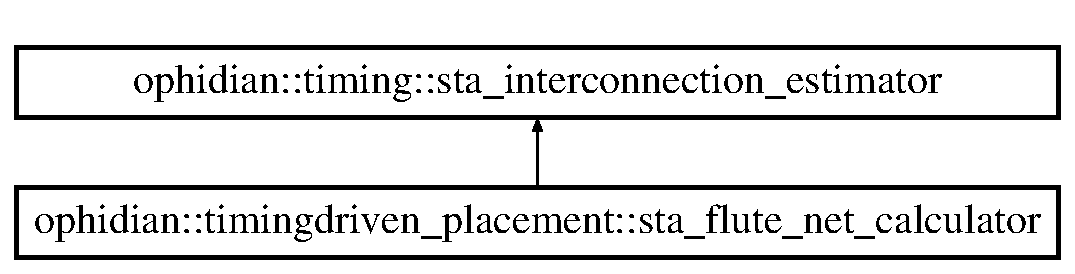
\includegraphics[height=2.000000cm]{classophidian_1_1timingdriven__placement_1_1sta__flute__net__calculator}
\end{center}
\end{figure}
\subsection*{Public Member Functions}
\begin{DoxyCompactItemize}
\item 
\hypertarget{classophidian_1_1timingdriven__placement_1_1sta__flute__net__calculator_a1808197d9d2e65f6bf2ad0f82123e766}{{\bfseries sta\-\_\-flute\-\_\-net\-\_\-calculator} (const \hyperlink{classophidian_1_1timing_1_1graph}{timing\-::graph} \&graph, const \hyperlink{classophidian_1_1placement_1_1placement}{placement\-::placement} \&placement, const \hyperlink{classophidian_1_1timing_1_1library}{timing\-::library} \&timing\-\_\-lib, \hyperlink{classophidian_1_1netlist_1_1netlist}{netlist\-::netlist} \&netlist)}\label{classophidian_1_1timingdriven__placement_1_1sta__flute__net__calculator_a1808197d9d2e65f6bf2ad0f82123e766}

\item 
\hypertarget{classophidian_1_1timingdriven__placement_1_1sta__flute__net__calculator_a5af3f771b140a743d01aabc7d0ef057f}{void {\bfseries update\-\_\-net} (\hyperlink{classophidian_1_1timing_1_1sta__timing__net__edge__calculator}{timing\-::sta\-\_\-timing\-\_\-net\-\_\-edge\-\_\-calculator} $\ast$tnet, entity\-\_\-system\-::entity net, \hyperlink{classophidian_1_1timing_1_1graph__nodes__timing}{timing\-::graph\-\_\-nodes\-\_\-timing} \&nodes\-\_\-timing)}\label{classophidian_1_1timingdriven__placement_1_1sta__flute__net__calculator_a5af3f771b140a743d01aabc7d0ef057f}

\end{DoxyCompactItemize}


The documentation for this class was generated from the following files\-:\begin{DoxyCompactItemize}
\item 
/home/csguth/workspace/openeda/src/timing-\/driven\-\_\-placement/sta\-\_\-flute\-\_\-net\-\_\-calculator.\-h\item 
/home/csguth/workspace/openeda/src/timing-\/driven\-\_\-placement/sta\-\_\-flute\-\_\-net\-\_\-calculator.\-cpp\end{DoxyCompactItemize}

\hypertarget{classophidian_1_1timing_1_1sta__interconnection__estimator}{\section{ophidian\-:\-:timing\-:\-:sta\-\_\-interconnection\-\_\-estimator Class Reference}
\label{classophidian_1_1timing_1_1sta__interconnection__estimator}\index{ophidian\-::timing\-::sta\-\_\-interconnection\-\_\-estimator@{ophidian\-::timing\-::sta\-\_\-interconnection\-\_\-estimator}}
}
Inheritance diagram for ophidian\-:\-:timing\-:\-:sta\-\_\-interconnection\-\_\-estimator\-:\begin{figure}[H]
\begin{center}
\leavevmode
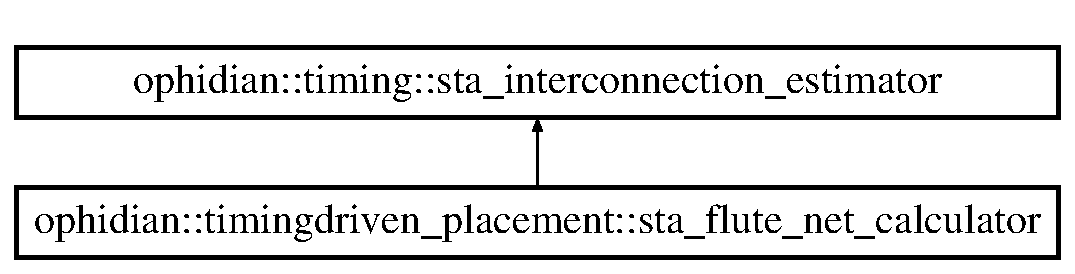
\includegraphics[height=2.000000cm]{classophidian_1_1timing_1_1sta__interconnection__estimator}
\end{center}
\end{figure}
\subsection*{Public Member Functions}
\begin{DoxyCompactItemize}
\item 
\hypertarget{classophidian_1_1timing_1_1sta__interconnection__estimator_a518eaf6cd4f65bdfcd559291537eff24}{virtual void {\bfseries update\-\_\-net} (\hyperlink{classophidian_1_1timing_1_1sta__timing__net__edge__calculator}{timing\-::sta\-\_\-timing\-\_\-net\-\_\-edge\-\_\-calculator} $\ast$tnet, entity\-\_\-system\-::entity net, \hyperlink{classophidian_1_1timing_1_1graph__nodes__timing}{timing\-::graph\-\_\-nodes\-\_\-timing} \&nodes\-\_\-timing)=0}\label{classophidian_1_1timing_1_1sta__interconnection__estimator_a518eaf6cd4f65bdfcd559291537eff24}

\end{DoxyCompactItemize}


The documentation for this class was generated from the following file\-:\begin{DoxyCompactItemize}
\item 
/home/csguth/workspace/openeda/src/timing/sta\-\_\-arc\-\_\-calculator.\-h\end{DoxyCompactItemize}

\hypertarget{classophidian_1_1timing_1_1sta__timing__arc__edge__calculator}{\section{ophidian\-:\-:timing\-:\-:sta\-\_\-timing\-\_\-arc\-\_\-edge\-\_\-calculator Class Reference}
\label{classophidian_1_1timing_1_1sta__timing__arc__edge__calculator}\index{ophidian\-::timing\-::sta\-\_\-timing\-\_\-arc\-\_\-edge\-\_\-calculator@{ophidian\-::timing\-::sta\-\_\-timing\-\_\-arc\-\_\-edge\-\_\-calculator}}
}
Inheritance diagram for ophidian\-:\-:timing\-:\-:sta\-\_\-timing\-\_\-arc\-\_\-edge\-\_\-calculator\-:\begin{figure}[H]
\begin{center}
\leavevmode
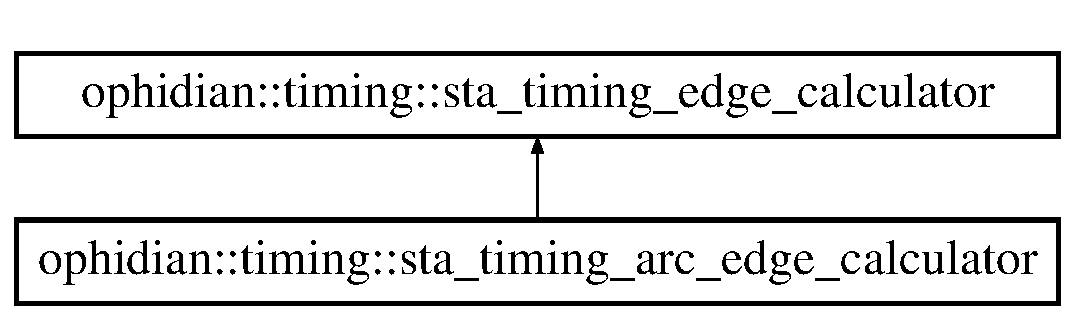
\includegraphics[height=2.000000cm]{classophidian_1_1timing_1_1sta__timing__arc__edge__calculator}
\end{center}
\end{figure}
\subsection*{Public Member Functions}
\begin{DoxyCompactItemize}
\item 
\hypertarget{classophidian_1_1timing_1_1sta__timing__arc__edge__calculator_aa2894632362a799075bec64cea5c0283}{{\bfseries sta\-\_\-timing\-\_\-arc\-\_\-edge\-\_\-calculator} (const \hyperlink{classophidian_1_1timing_1_1library}{library} \&lib)}\label{classophidian_1_1timing_1_1sta__timing__arc__edge__calculator_aa2894632362a799075bec64cea5c0283}

\item 
\hypertarget{classophidian_1_1timing_1_1sta__timing__arc__edge__calculator_a1d0e6c4d58f62b9c6fc7622d45b6e119}{void {\bfseries update} (const \hyperlink{classophidian_1_1timing_1_1graph}{graph} \&g, const graph\-::edge arc, const \hyperlink{classophidian_1_1timing_1_1graph__nodes__timing}{graph\-\_\-nodes\-\_\-timing} \&nodes, \hyperlink{classophidian_1_1timing_1_1graph__arcs__timing}{graph\-\_\-arcs\-\_\-timing} \&arcs)}\label{classophidian_1_1timing_1_1sta__timing__arc__edge__calculator_a1d0e6c4d58f62b9c6fc7622d45b6e119}

\end{DoxyCompactItemize}


The documentation for this class was generated from the following files\-:\begin{DoxyCompactItemize}
\item 
/home/renan/workspace/openeda/src/timing/sta\-\_\-arc\-\_\-calculator.\-h\item 
/home/renan/workspace/openeda/src/timing/sta\-\_\-arc\-\_\-calculator.\-cpp\end{DoxyCompactItemize}

\hypertarget{classophidian_1_1timing_1_1sta__timing__edge__calculator}{\section{ophidian\-:\-:timing\-:\-:sta\-\_\-timing\-\_\-edge\-\_\-calculator Class Reference}
\label{classophidian_1_1timing_1_1sta__timing__edge__calculator}\index{ophidian\-::timing\-::sta\-\_\-timing\-\_\-edge\-\_\-calculator@{ophidian\-::timing\-::sta\-\_\-timing\-\_\-edge\-\_\-calculator}}
}
Inheritance diagram for ophidian\-:\-:timing\-:\-:sta\-\_\-timing\-\_\-edge\-\_\-calculator\-:\begin{figure}[H]
\begin{center}
\leavevmode
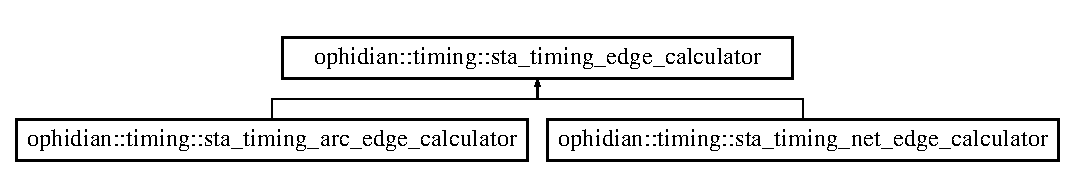
\includegraphics[height=1.924399cm]{classophidian_1_1timing_1_1sta__timing__edge__calculator}
\end{center}
\end{figure}
\subsection*{Public Member Functions}
\begin{DoxyCompactItemize}
\item 
\hypertarget{classophidian_1_1timing_1_1sta__timing__edge__calculator_a1621f0c51ed5b6a9ffcc9456a10d1645}{virtual void {\bfseries update} (const \hyperlink{classophidian_1_1timing_1_1graph}{graph} \&g, const graph\-::edge arc, const \hyperlink{classophidian_1_1timing_1_1graph__nodes__timing}{graph\-\_\-nodes\-\_\-timing} \&nodes, \hyperlink{classophidian_1_1timing_1_1graph__arcs__timing}{graph\-\_\-arcs\-\_\-timing} \&arcs)=0}\label{classophidian_1_1timing_1_1sta__timing__edge__calculator_a1621f0c51ed5b6a9ffcc9456a10d1645}

\end{DoxyCompactItemize}


The documentation for this class was generated from the following file\-:\begin{DoxyCompactItemize}
\item 
/home/csguth/workspace/openeda/src/timing/sta\-\_\-arc\-\_\-calculator.\-h\end{DoxyCompactItemize}

\hypertarget{classophidian_1_1timing_1_1sta__timing__net__edge__calculator}{\section{ophidian\-:\-:timing\-:\-:sta\-\_\-timing\-\_\-net\-\_\-edge\-\_\-calculator Class Reference}
\label{classophidian_1_1timing_1_1sta__timing__net__edge__calculator}\index{ophidian\-::timing\-::sta\-\_\-timing\-\_\-net\-\_\-edge\-\_\-calculator@{ophidian\-::timing\-::sta\-\_\-timing\-\_\-net\-\_\-edge\-\_\-calculator}}
}
Inheritance diagram for ophidian\-:\-:timing\-:\-:sta\-\_\-timing\-\_\-net\-\_\-edge\-\_\-calculator\-:\begin{figure}[H]
\begin{center}
\leavevmode
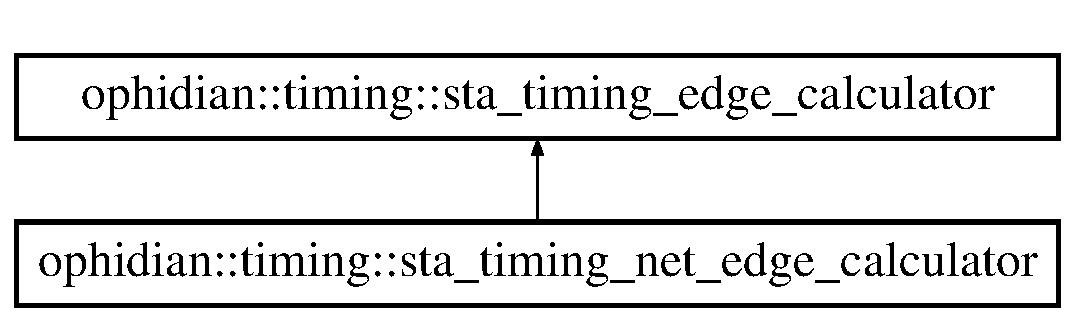
\includegraphics[height=2.000000cm]{classophidian_1_1timing_1_1sta__timing__net__edge__calculator}
\end{center}
\end{figure}
\subsection*{Public Member Functions}
\begin{DoxyCompactItemize}
\item 
\hypertarget{classophidian_1_1timing_1_1sta__timing__net__edge__calculator_a3ffa2d1f1277e2710244d369b6a1b43b}{{\bfseries sta\-\_\-timing\-\_\-net\-\_\-edge\-\_\-calculator} (const \hyperlink{classophidian_1_1timing_1_1graph}{graph} \&g)}\label{classophidian_1_1timing_1_1sta__timing__net__edge__calculator_a3ffa2d1f1277e2710244d369b6a1b43b}

\item 
\hypertarget{classophidian_1_1timing_1_1sta__timing__net__edge__calculator_ae32b4f4ac34c93696461cfa9b522d637}{void {\bfseries elmore\-\_\-delay} (lemon\-::\-List\-Digraph\-::\-Node node, boost\-::units\-::quantity$<$ boost\-::units\-::si\-::time $>$ delay)}\label{classophidian_1_1timing_1_1sta__timing__net__edge__calculator_ae32b4f4ac34c93696461cfa9b522d637}

\item 
\hypertarget{classophidian_1_1timing_1_1sta__timing__net__edge__calculator_af4a5d464ed082b9eaf1a2b66f6773e19}{void {\bfseries elmore\-\_\-slew} (lemon\-::\-List\-Digraph\-::\-Node node, boost\-::units\-::quantity$<$ boost\-::units\-::si\-::time $>$ slew)}\label{classophidian_1_1timing_1_1sta__timing__net__edge__calculator_af4a5d464ed082b9eaf1a2b66f6773e19}

\item 
\hypertarget{classophidian_1_1timing_1_1sta__timing__net__edge__calculator_ae86054b615d75b84346404dc87489b82}{void {\bfseries update} (const \hyperlink{classophidian_1_1timing_1_1graph}{graph} \&g, const graph\-::edge arc, const \hyperlink{classophidian_1_1timing_1_1graph__nodes__timing}{graph\-\_\-nodes\-\_\-timing} \&nodes, \hyperlink{classophidian_1_1timing_1_1graph__arcs__timing}{graph\-\_\-arcs\-\_\-timing} \&arcs)}\label{classophidian_1_1timing_1_1sta__timing__net__edge__calculator_ae86054b615d75b84346404dc87489b82}

\end{DoxyCompactItemize}


The documentation for this class was generated from the following files\-:\begin{DoxyCompactItemize}
\item 
/home/renan/workspace/openeda/src/timing/sta\-\_\-arc\-\_\-calculator.\-h\item 
/home/renan/workspace/openeda/src/timing/sta\-\_\-arc\-\_\-calculator.\-cpp\end{DoxyCompactItemize}

\hypertarget{classophidian_1_1timing_1_1sta__timing__point__calculator}{\section{ophidian\-:\-:timing\-:\-:sta\-\_\-timing\-\_\-point\-\_\-calculator Class Reference}
\label{classophidian_1_1timing_1_1sta__timing__point__calculator}\index{ophidian\-::timing\-::sta\-\_\-timing\-\_\-point\-\_\-calculator@{ophidian\-::timing\-::sta\-\_\-timing\-\_\-point\-\_\-calculator}}
}
\subsection*{Public Member Functions}
\begin{DoxyCompactItemize}
\item 
\hypertarget{classophidian_1_1timing_1_1sta__timing__point__calculator_a66fdb10df8fd86b47f30564aba9427bb}{{\bfseries sta\-\_\-timing\-\_\-point\-\_\-calculator} (const \hyperlink{classophidian_1_1timing_1_1graph}{graph} \&g)}\label{classophidian_1_1timing_1_1sta__timing__point__calculator_a66fdb10df8fd86b47f30564aba9427bb}

\item 
\hypertarget{classophidian_1_1timing_1_1sta__timing__point__calculator_a48d5fe5559e3c2deef2a0172b0300448}{void {\bfseries reset\-\_\-counter} ()}\label{classophidian_1_1timing_1_1sta__timing__point__calculator_a48d5fe5559e3c2deef2a0172b0300448}

\item 
\hypertarget{classophidian_1_1timing_1_1sta__timing__point__calculator_a538cc055479c5e5fa73b2f41f3536558}{bool {\bfseries empty} ()}\label{classophidian_1_1timing_1_1sta__timing__point__calculator_a538cc055479c5e5fa73b2f41f3536558}

\item 
\hypertarget{classophidian_1_1timing_1_1sta__timing__point__calculator_a7d92d877d754d774025d5e2acc641318}{virtual void {\bfseries push} (lemon\-::\-List\-Digraph\-::\-Node node)}\label{classophidian_1_1timing_1_1sta__timing__point__calculator_a7d92d877d754d774025d5e2acc641318}

\item 
virtual void \hyperlink{classophidian_1_1timing_1_1sta__timing__point__calculator_ab02dcda032d2166dcf47f36e3554fd08}{process\-\_\-queue} (const \hyperlink{classophidian_1_1timing_1_1graph}{graph} \&m\-\_\-graph, const \hyperlink{classophidian_1_1timing_1_1graph__arcs__timing}{graph\-\_\-arcs\-\_\-timing} \&m\-\_\-arcs\-\_\-timing, \hyperlink{classophidian_1_1timing_1_1graph__nodes__timing}{graph\-\_\-nodes\-\_\-timing} \&m\-\_\-nodes\-\_\-timing, lemon\-::\-List\-Digraph\-::\-Arc\-Map$<$ \hyperlink{classophidian_1_1timing_1_1sta__timing__edge__calculator}{sta\-\_\-timing\-\_\-edge\-\_\-calculator} $\ast$ $>$ \&tarcs)
\end{DoxyCompactItemize}


\subsection{Member Function Documentation}
\hypertarget{classophidian_1_1timing_1_1sta__timing__point__calculator_ab02dcda032d2166dcf47f36e3554fd08}{\index{ophidian\-::timing\-::sta\-\_\-timing\-\_\-point\-\_\-calculator@{ophidian\-::timing\-::sta\-\_\-timing\-\_\-point\-\_\-calculator}!process\-\_\-queue@{process\-\_\-queue}}
\index{process\-\_\-queue@{process\-\_\-queue}!ophidian::timing::sta_timing_point_calculator@{ophidian\-::timing\-::sta\-\_\-timing\-\_\-point\-\_\-calculator}}
\subsubsection[{process\-\_\-queue}]{\setlength{\rightskip}{0pt plus 5cm}void openeda\-::timing\-::sta\-\_\-timing\-\_\-point\-\_\-calculator\-::process\-\_\-queue (
\begin{DoxyParamCaption}
\item[{const {\bf graph} \&}]{m\-\_\-graph, }
\item[{const {\bf graph\-\_\-arcs\-\_\-timing} \&}]{m\-\_\-arcs\-\_\-timing, }
\item[{{\bf graph\-\_\-nodes\-\_\-timing} \&}]{m\-\_\-nodes\-\_\-timing, }
\item[{lemon\-::\-List\-Digraph\-::\-Arc\-Map$<$ {\bf sta\-\_\-timing\-\_\-edge\-\_\-calculator} $\ast$ $>$ \&}]{tarcs}
\end{DoxyParamCaption}
)\hspace{0.3cm}{\ttfamily [virtual]}}}\label{classophidian_1_1timing_1_1sta__timing__point__calculator_ab02dcda032d2166dcf47f36e3554fd08}
$<$$<$$<$$<$ 

The documentation for this class was generated from the following files\-:\begin{DoxyCompactItemize}
\item 
/home/csguth/workspace/openeda/src/timing/sta\-\_\-timing\-\_\-point\-\_\-calculator.\-h\item 
/home/csguth/workspace/openeda/src/timing/sta\-\_\-timing\-\_\-point\-\_\-calculator.\-cpp\end{DoxyCompactItemize}

\hypertarget{classophidian_1_1standard__cell_1_1standard__cells}{\section{ophidian\-:\-:standard\-\_\-cell\-:\-:standard\-\_\-cells Class Reference}
\label{classophidian_1_1standard__cell_1_1standard__cells}\index{ophidian\-::standard\-\_\-cell\-::standard\-\_\-cells@{ophidian\-::standard\-\_\-cell\-::standard\-\_\-cells}}
}


Standard cell class.  




{\ttfamily \#include $<$standard\-\_\-cells.\-h$>$}

\subsection*{Public Member Functions}
\begin{DoxyCompactItemize}
\item 
\hyperlink{classophidian_1_1standard__cell_1_1standard__cells_a550904ff92dda77064942532e4ffb0cd}{standard\-\_\-cells} ()
\begin{DoxyCompactList}\small\item\em Constructor. \end{DoxyCompactList}\item 
void \hyperlink{classophidian_1_1standard__cell_1_1standard__cells_ad2320be742c38f15a3bf267a829f1ea6}{register\-\_\-cell\-\_\-property} (\hyperlink{classophidian_1_1entity_1_1property}{entity\-::property} $\ast$property)
\begin{DoxyCompactList}\small\item\em Registers cell property. \end{DoxyCompactList}\item 
void \hyperlink{classophidian_1_1standard__cell_1_1standard__cells_ab3736094116a3730c9beef2cef923021}{register\-\_\-pin\-\_\-property} (\hyperlink{classophidian_1_1entity_1_1property}{entity\-::property} $\ast$property)
\begin{DoxyCompactList}\small\item\em Registers pin property. \end{DoxyCompactList}\item 
const \hyperlink{classophidian_1_1entity_1_1vector__property}{entity\-::vector\-\_\-property}\\*
$<$ std\-::string $>$ \& \hyperlink{classophidian_1_1standard__cell_1_1standard__cells_a8fdfdb96a4173eb0881287f3ad8c191b}{cell\-\_\-names} () const 
\begin{DoxyCompactList}\small\item\em Cell names getter. \end{DoxyCompactList}\item 
\hyperlink{classophidian_1_1entity_1_1entity}{entity\-::entity} \hyperlink{classophidian_1_1standard__cell_1_1standard__cells_ac4b65b059e571d86bfbad04132bc29b9}{cell\-\_\-create} (std\-::string name)
\begin{DoxyCompactList}\small\item\em Creates a cell. \end{DoxyCompactList}\item 
std\-::string \hyperlink{classophidian_1_1standard__cell_1_1standard__cells_aa5953f7a39220cdfad7871d4cd34f2e9}{cell\-\_\-name} (\hyperlink{classophidian_1_1entity_1_1entity}{entity\-::entity} cell) const 
\begin{DoxyCompactList}\small\item\em Cell name getter. \end{DoxyCompactList}\item 
const std\-::vector\\*
$<$ \hyperlink{classophidian_1_1entity_1_1entity}{entity\-::entity} $>$ \& \hyperlink{classophidian_1_1standard__cell_1_1standard__cells_a0a6ad5354545086741534e1e5b963c61}{cell\-\_\-pins} (\hyperlink{classophidian_1_1entity_1_1entity}{entity\-::entity} cell) const 
\begin{DoxyCompactList}\small\item\em Cell pins getter. \end{DoxyCompactList}\item 
std\-::size\-\_\-t \hyperlink{classophidian_1_1standard__cell_1_1standard__cells_a704442c2289df257ab5cd779f1307eef}{cell\-\_\-count} () const 
\begin{DoxyCompactList}\small\item\em Returns the number of cells. \end{DoxyCompactList}\item 
const \hyperlink{classophidian_1_1entity_1_1system}{entity\-::system} \& \hyperlink{classophidian_1_1standard__cell_1_1standard__cells_a8c7ca7d653866b880df97a8f7b6998fb}{cell\-\_\-system} () const 
\begin{DoxyCompactList}\small\item\em Cell system getter. \end{DoxyCompactList}\item 
void \hyperlink{classophidian_1_1standard__cell_1_1standard__cells_a838f7cf223b913a996e0eb175a8ef4ae}{cell\-\_\-sequential} (\hyperlink{classophidian_1_1entity_1_1entity}{entity\-::entity} cell, bool sequential)
\begin{DoxyCompactList}\small\item\em Cell sequential attribute setter. \end{DoxyCompactList}\item 
bool \hyperlink{classophidian_1_1standard__cell_1_1standard__cells_a32f67b146acf6e185a54fb7e3e2711a5}{cell\-\_\-sequential} (\hyperlink{classophidian_1_1entity_1_1entity}{entity\-::entity} cell) const 
\begin{DoxyCompactList}\small\item\em Cell sequential attribute getter. \end{DoxyCompactList}\item 
\hyperlink{classophidian_1_1entity_1_1entity}{entity\-::entity} \hyperlink{classophidian_1_1standard__cell_1_1standard__cells_a38cf47d034e65203af44d506c0c536c8}{pin\-\_\-create} (\hyperlink{classophidian_1_1entity_1_1entity}{entity\-::entity} cell, std\-::string name)
\begin{DoxyCompactList}\small\item\em Creates a pin. \end{DoxyCompactList}\item 
\hyperlink{classophidian_1_1entity_1_1entity}{entity\-::entity} \hyperlink{classophidian_1_1standard__cell_1_1standard__cells_ababb1f68b313bbf202aeb63c2b113ef5}{pin\-\_\-owner} (\hyperlink{classophidian_1_1entity_1_1entity}{entity\-::entity} pin) const 
\begin{DoxyCompactList}\small\item\em Pin owner getter. \end{DoxyCompactList}\item 
std\-::string \hyperlink{classophidian_1_1standard__cell_1_1standard__cells_a3a8ff3bb3df8f3c5c77835c99a8d376f}{pin\-\_\-name} (\hyperlink{classophidian_1_1entity_1_1entity}{entity\-::entity} pin) const 
\begin{DoxyCompactList}\small\item\em Pin name getter. \end{DoxyCompactList}\item 
std\-::size\-\_\-t \hyperlink{classophidian_1_1standard__cell_1_1standard__cells_a144aaa53cc5d9808f5d26d51b76fad01}{pin\-\_\-count} () const 
\begin{DoxyCompactList}\small\item\em Returns the number of pins. \end{DoxyCompactList}\item 
const \hyperlink{classophidian_1_1entity_1_1system}{entity\-::system} \& \hyperlink{classophidian_1_1standard__cell_1_1standard__cells_acc1ac0ae7c27a535ac8922d7d7d12581}{pin\-\_\-system} () const 
\begin{DoxyCompactList}\small\item\em Pin system getter. \end{DoxyCompactList}\item 
pin\-\_\-directions \hyperlink{classophidian_1_1standard__cell_1_1standard__cells_a7bab4c82de4b402ec7853befa34696e2}{pin\-\_\-direction} (\hyperlink{classophidian_1_1entity_1_1entity}{entity\-::entity} pin) const 
\begin{DoxyCompactList}\small\item\em Pin direction getter. \end{DoxyCompactList}\item 
bool \hyperlink{classophidian_1_1standard__cell_1_1standard__cells_a3e31812d8491b1dfd8508c27a4568146}{pin\-\_\-clock\-\_\-input} (\hyperlink{classophidian_1_1entity_1_1entity}{entity\-::entity} pin) const 
\begin{DoxyCompactList}\small\item\em Pin clock input attribute getter. \end{DoxyCompactList}\item 
void \hyperlink{classophidian_1_1standard__cell_1_1standard__cells_a6bf78038d710a46f9ae3408612528cc8}{pin\-\_\-clock\-\_\-input} (\hyperlink{classophidian_1_1entity_1_1entity}{entity\-::entity} pin, bool clock\-\_\-input)
\begin{DoxyCompactList}\small\item\em Pin clock input attribute setter. \end{DoxyCompactList}\item 
void \hyperlink{classophidian_1_1standard__cell_1_1standard__cells_a04ff23c3a93a8e2d029c4078b59dc2d5}{pin\-\_\-direction} (\hyperlink{classophidian_1_1entity_1_1entity}{entity\-::entity} pin, pin\-\_\-directions direction)
\begin{DoxyCompactList}\small\item\em Pin direction setter. \end{DoxyCompactList}\item 
\hyperlink{classophidian_1_1entity_1_1entity}{entity\-::entity} \hyperlink{classophidian_1_1standard__cell_1_1standard__cells_aa244a3aacf05477fb08056a82caaff0f}{pad\-\_\-create} (std\-::string name)
\begin{DoxyCompactList}\small\item\em Creates a pad. \end{DoxyCompactList}\end{DoxyCompactItemize}


\subsection{Detailed Description}
This class provides the basic standard cell interface, such as creation of cell and pin types. 

\subsection{Constructor \& Destructor Documentation}
\hypertarget{classophidian_1_1standard__cell_1_1standard__cells_a550904ff92dda77064942532e4ffb0cd}{\index{ophidian\-::standard\-\_\-cell\-::standard\-\_\-cells@{ophidian\-::standard\-\_\-cell\-::standard\-\_\-cells}!standard\-\_\-cells@{standard\-\_\-cells}}
\index{standard\-\_\-cells@{standard\-\_\-cells}!ophidian::standard_cell::standard_cells@{ophidian\-::standard\-\_\-cell\-::standard\-\_\-cells}}
\subsubsection[{standard\-\_\-cells}]{\setlength{\rightskip}{0pt plus 5cm}ophidian\-::standard\-\_\-cell\-::standard\-\_\-cells\-::standard\-\_\-cells (
\begin{DoxyParamCaption}
{}
\end{DoxyParamCaption}
)}}\label{classophidian_1_1standard__cell_1_1standard__cells_a550904ff92dda77064942532e4ffb0cd}
Default constructor of the standard cell class. Initializes an empty system for cells and pins. 

\subsection{Member Function Documentation}
\hypertarget{classophidian_1_1standard__cell_1_1standard__cells_a704442c2289df257ab5cd779f1307eef}{\index{ophidian\-::standard\-\_\-cell\-::standard\-\_\-cells@{ophidian\-::standard\-\_\-cell\-::standard\-\_\-cells}!cell\-\_\-count@{cell\-\_\-count}}
\index{cell\-\_\-count@{cell\-\_\-count}!ophidian::standard_cell::standard_cells@{ophidian\-::standard\-\_\-cell\-::standard\-\_\-cells}}
\subsubsection[{cell\-\_\-count}]{\setlength{\rightskip}{0pt plus 5cm}std\-::size\-\_\-t ophidian\-::standard\-\_\-cell\-::standard\-\_\-cells\-::cell\-\_\-count (
\begin{DoxyParamCaption}
{}
\end{DoxyParamCaption}
) const\hspace{0.3cm}{\ttfamily [inline]}}}\label{classophidian_1_1standard__cell_1_1standard__cells_a704442c2289df257ab5cd779f1307eef}
Returns the number of cells created in the cells system. \begin{DoxyReturn}{Returns}
Number of cells. 
\end{DoxyReturn}
\hypertarget{classophidian_1_1standard__cell_1_1standard__cells_ac4b65b059e571d86bfbad04132bc29b9}{\index{ophidian\-::standard\-\_\-cell\-::standard\-\_\-cells@{ophidian\-::standard\-\_\-cell\-::standard\-\_\-cells}!cell\-\_\-create@{cell\-\_\-create}}
\index{cell\-\_\-create@{cell\-\_\-create}!ophidian::standard_cell::standard_cells@{ophidian\-::standard\-\_\-cell\-::standard\-\_\-cells}}
\subsubsection[{cell\-\_\-create}]{\setlength{\rightskip}{0pt plus 5cm}{\bf entity\-::entity} ophidian\-::standard\-\_\-cell\-::standard\-\_\-cells\-::cell\-\_\-create (
\begin{DoxyParamCaption}
\item[{std\-::string}]{name}
\end{DoxyParamCaption}
)}}\label{classophidian_1_1standard__cell_1_1standard__cells_ac4b65b059e571d86bfbad04132bc29b9}
Creates a new cell in the standard cell library. 
\begin{DoxyParams}{Parameters}
{\em name} & Name of the new cell. \\
\hline
\end{DoxyParams}
\begin{DoxyReturn}{Returns}
Entity of the created cell. 
\end{DoxyReturn}
\hypertarget{classophidian_1_1standard__cell_1_1standard__cells_aa5953f7a39220cdfad7871d4cd34f2e9}{\index{ophidian\-::standard\-\_\-cell\-::standard\-\_\-cells@{ophidian\-::standard\-\_\-cell\-::standard\-\_\-cells}!cell\-\_\-name@{cell\-\_\-name}}
\index{cell\-\_\-name@{cell\-\_\-name}!ophidian::standard_cell::standard_cells@{ophidian\-::standard\-\_\-cell\-::standard\-\_\-cells}}
\subsubsection[{cell\-\_\-name}]{\setlength{\rightskip}{0pt plus 5cm}std\-::string ophidian\-::standard\-\_\-cell\-::standard\-\_\-cells\-::cell\-\_\-name (
\begin{DoxyParamCaption}
\item[{{\bf entity\-::entity}}]{cell}
\end{DoxyParamCaption}
) const\hspace{0.3cm}{\ttfamily [inline]}}}\label{classophidian_1_1standard__cell_1_1standard__cells_aa5953f7a39220cdfad7871d4cd34f2e9}
Returns the name of a cell. 
\begin{DoxyParams}{Parameters}
{\em cell} & Cell entity to get the name. \\
\hline
\end{DoxyParams}
\begin{DoxyReturn}{Returns}
Name of the cell. 
\end{DoxyReturn}
\hypertarget{classophidian_1_1standard__cell_1_1standard__cells_a8fdfdb96a4173eb0881287f3ad8c191b}{\index{ophidian\-::standard\-\_\-cell\-::standard\-\_\-cells@{ophidian\-::standard\-\_\-cell\-::standard\-\_\-cells}!cell\-\_\-names@{cell\-\_\-names}}
\index{cell\-\_\-names@{cell\-\_\-names}!ophidian::standard_cell::standard_cells@{ophidian\-::standard\-\_\-cell\-::standard\-\_\-cells}}
\subsubsection[{cell\-\_\-names}]{\setlength{\rightskip}{0pt plus 5cm}const {\bf entity\-::vector\-\_\-property}$<$std\-::string$>$\& ophidian\-::standard\-\_\-cell\-::standard\-\_\-cells\-::cell\-\_\-names (
\begin{DoxyParamCaption}
{}
\end{DoxyParamCaption}
) const\hspace{0.3cm}{\ttfamily [inline]}}}\label{classophidian_1_1standard__cell_1_1standard__cells_a8fdfdb96a4173eb0881287f3ad8c191b}
Returns the names of all cells. \begin{DoxyReturn}{Returns}
Constant reference to the cell names property. 
\end{DoxyReturn}
\hypertarget{classophidian_1_1standard__cell_1_1standard__cells_a0a6ad5354545086741534e1e5b963c61}{\index{ophidian\-::standard\-\_\-cell\-::standard\-\_\-cells@{ophidian\-::standard\-\_\-cell\-::standard\-\_\-cells}!cell\-\_\-pins@{cell\-\_\-pins}}
\index{cell\-\_\-pins@{cell\-\_\-pins}!ophidian::standard_cell::standard_cells@{ophidian\-::standard\-\_\-cell\-::standard\-\_\-cells}}
\subsubsection[{cell\-\_\-pins}]{\setlength{\rightskip}{0pt plus 5cm}const std\-::vector$<${\bf entity\-::entity}$>$\& ophidian\-::standard\-\_\-cell\-::standard\-\_\-cells\-::cell\-\_\-pins (
\begin{DoxyParamCaption}
\item[{{\bf entity\-::entity}}]{cell}
\end{DoxyParamCaption}
) const\hspace{0.3cm}{\ttfamily [inline]}}}\label{classophidian_1_1standard__cell_1_1standard__cells_a0a6ad5354545086741534e1e5b963c61}
Returns the pins of a cell. 
\begin{DoxyParams}{Parameters}
{\em cell} & Cell entity to get the pins. \\
\hline
\end{DoxyParams}
\begin{DoxyReturn}{Returns}
Constant reference to a vector with all pins of that cell. 
\end{DoxyReturn}
\hypertarget{classophidian_1_1standard__cell_1_1standard__cells_a838f7cf223b913a996e0eb175a8ef4ae}{\index{ophidian\-::standard\-\_\-cell\-::standard\-\_\-cells@{ophidian\-::standard\-\_\-cell\-::standard\-\_\-cells}!cell\-\_\-sequential@{cell\-\_\-sequential}}
\index{cell\-\_\-sequential@{cell\-\_\-sequential}!ophidian::standard_cell::standard_cells@{ophidian\-::standard\-\_\-cell\-::standard\-\_\-cells}}
\subsubsection[{cell\-\_\-sequential}]{\setlength{\rightskip}{0pt plus 5cm}void ophidian\-::standard\-\_\-cell\-::standard\-\_\-cells\-::cell\-\_\-sequential (
\begin{DoxyParamCaption}
\item[{{\bf entity\-::entity}}]{cell, }
\item[{bool}]{sequential}
\end{DoxyParamCaption}
)}}\label{classophidian_1_1standard__cell_1_1standard__cells_a838f7cf223b913a996e0eb175a8ef4ae}
Sets if a cell is a sequential cell. 
\begin{DoxyParams}{Parameters}
{\em cell} & Cell entity to be set. \\
\hline
{\em sequential} & bool variable describing if the cell is sequential or not. \\
\hline
\end{DoxyParams}
\hypertarget{classophidian_1_1standard__cell_1_1standard__cells_a32f67b146acf6e185a54fb7e3e2711a5}{\index{ophidian\-::standard\-\_\-cell\-::standard\-\_\-cells@{ophidian\-::standard\-\_\-cell\-::standard\-\_\-cells}!cell\-\_\-sequential@{cell\-\_\-sequential}}
\index{cell\-\_\-sequential@{cell\-\_\-sequential}!ophidian::standard_cell::standard_cells@{ophidian\-::standard\-\_\-cell\-::standard\-\_\-cells}}
\subsubsection[{cell\-\_\-sequential}]{\setlength{\rightskip}{0pt plus 5cm}bool ophidian\-::standard\-\_\-cell\-::standard\-\_\-cells\-::cell\-\_\-sequential (
\begin{DoxyParamCaption}
\item[{{\bf entity\-::entity}}]{cell}
\end{DoxyParamCaption}
) const\hspace{0.3cm}{\ttfamily [inline]}}}\label{classophidian_1_1standard__cell_1_1standard__cells_a32f67b146acf6e185a54fb7e3e2711a5}
Gets if a cell is a sequential cell. 
\begin{DoxyParams}{Parameters}
{\em cell} & Cell entity to get the attribute. \\
\hline
\end{DoxyParams}
\begin{DoxyReturn}{Returns}
bool variable describing if the cell is sequential or not. 
\end{DoxyReturn}
\hypertarget{classophidian_1_1standard__cell_1_1standard__cells_a8c7ca7d653866b880df97a8f7b6998fb}{\index{ophidian\-::standard\-\_\-cell\-::standard\-\_\-cells@{ophidian\-::standard\-\_\-cell\-::standard\-\_\-cells}!cell\-\_\-system@{cell\-\_\-system}}
\index{cell\-\_\-system@{cell\-\_\-system}!ophidian::standard_cell::standard_cells@{ophidian\-::standard\-\_\-cell\-::standard\-\_\-cells}}
\subsubsection[{cell\-\_\-system}]{\setlength{\rightskip}{0pt plus 5cm}const {\bf entity\-::system}\& ophidian\-::standard\-\_\-cell\-::standard\-\_\-cells\-::cell\-\_\-system (
\begin{DoxyParamCaption}
{}
\end{DoxyParamCaption}
) const\hspace{0.3cm}{\ttfamily [inline]}}}\label{classophidian_1_1standard__cell_1_1standard__cells_a8c7ca7d653866b880df97a8f7b6998fb}
Returns the cell system. \begin{DoxyReturn}{Returns}
Constant reference to the cell system. 
\end{DoxyReturn}
\hypertarget{classophidian_1_1standard__cell_1_1standard__cells_aa244a3aacf05477fb08056a82caaff0f}{\index{ophidian\-::standard\-\_\-cell\-::standard\-\_\-cells@{ophidian\-::standard\-\_\-cell\-::standard\-\_\-cells}!pad\-\_\-create@{pad\-\_\-create}}
\index{pad\-\_\-create@{pad\-\_\-create}!ophidian::standard_cell::standard_cells@{ophidian\-::standard\-\_\-cell\-::standard\-\_\-cells}}
\subsubsection[{pad\-\_\-create}]{\setlength{\rightskip}{0pt plus 5cm}{\bf entity\-::entity} ophidian\-::standard\-\_\-cell\-::standard\-\_\-cells\-::pad\-\_\-create (
\begin{DoxyParamCaption}
\item[{std\-::string}]{name}
\end{DoxyParamCaption}
)}}\label{classophidian_1_1standard__cell_1_1standard__cells_aa244a3aacf05477fb08056a82caaff0f}
Creates a new pad in the standard cell library. A pad is a special pin without owner. 
\begin{DoxyParams}{Parameters}
{\em name} & Name of the new pad. \\
\hline
\end{DoxyParams}
\begin{DoxyReturn}{Returns}
Entity of the created pad. 
\end{DoxyReturn}
\hypertarget{classophidian_1_1standard__cell_1_1standard__cells_a3e31812d8491b1dfd8508c27a4568146}{\index{ophidian\-::standard\-\_\-cell\-::standard\-\_\-cells@{ophidian\-::standard\-\_\-cell\-::standard\-\_\-cells}!pin\-\_\-clock\-\_\-input@{pin\-\_\-clock\-\_\-input}}
\index{pin\-\_\-clock\-\_\-input@{pin\-\_\-clock\-\_\-input}!ophidian::standard_cell::standard_cells@{ophidian\-::standard\-\_\-cell\-::standard\-\_\-cells}}
\subsubsection[{pin\-\_\-clock\-\_\-input}]{\setlength{\rightskip}{0pt plus 5cm}bool ophidian\-::standard\-\_\-cell\-::standard\-\_\-cells\-::pin\-\_\-clock\-\_\-input (
\begin{DoxyParamCaption}
\item[{{\bf entity\-::entity}}]{pin}
\end{DoxyParamCaption}
) const\hspace{0.3cm}{\ttfamily [inline]}}}\label{classophidian_1_1standard__cell_1_1standard__cells_a3e31812d8491b1dfd8508c27a4568146}
Gets if a pin is a clock input. 
\begin{DoxyParams}{Parameters}
{\em pin} & Pin entity to get the attribute. \\
\hline
\end{DoxyParams}
\begin{DoxyReturn}{Returns}
bool variable describing if the pin is a clock input or not. 
\end{DoxyReturn}
\hypertarget{classophidian_1_1standard__cell_1_1standard__cells_a6bf78038d710a46f9ae3408612528cc8}{\index{ophidian\-::standard\-\_\-cell\-::standard\-\_\-cells@{ophidian\-::standard\-\_\-cell\-::standard\-\_\-cells}!pin\-\_\-clock\-\_\-input@{pin\-\_\-clock\-\_\-input}}
\index{pin\-\_\-clock\-\_\-input@{pin\-\_\-clock\-\_\-input}!ophidian::standard_cell::standard_cells@{ophidian\-::standard\-\_\-cell\-::standard\-\_\-cells}}
\subsubsection[{pin\-\_\-clock\-\_\-input}]{\setlength{\rightskip}{0pt plus 5cm}void ophidian\-::standard\-\_\-cell\-::standard\-\_\-cells\-::pin\-\_\-clock\-\_\-input (
\begin{DoxyParamCaption}
\item[{{\bf entity\-::entity}}]{pin, }
\item[{bool}]{clock\-\_\-input}
\end{DoxyParamCaption}
)}}\label{classophidian_1_1standard__cell_1_1standard__cells_a6bf78038d710a46f9ae3408612528cc8}
Sets if a pin is a clock input. 
\begin{DoxyParams}{Parameters}
{\em pin} & Pin entity to be set. \\
\hline
{\em clock\-\_\-input} & bool variable describing if the pin is a clock input or not. \\
\hline
\end{DoxyParams}
\hypertarget{classophidian_1_1standard__cell_1_1standard__cells_a144aaa53cc5d9808f5d26d51b76fad01}{\index{ophidian\-::standard\-\_\-cell\-::standard\-\_\-cells@{ophidian\-::standard\-\_\-cell\-::standard\-\_\-cells}!pin\-\_\-count@{pin\-\_\-count}}
\index{pin\-\_\-count@{pin\-\_\-count}!ophidian::standard_cell::standard_cells@{ophidian\-::standard\-\_\-cell\-::standard\-\_\-cells}}
\subsubsection[{pin\-\_\-count}]{\setlength{\rightskip}{0pt plus 5cm}std\-::size\-\_\-t ophidian\-::standard\-\_\-cell\-::standard\-\_\-cells\-::pin\-\_\-count (
\begin{DoxyParamCaption}
{}
\end{DoxyParamCaption}
) const\hspace{0.3cm}{\ttfamily [inline]}}}\label{classophidian_1_1standard__cell_1_1standard__cells_a144aaa53cc5d9808f5d26d51b76fad01}
Returns the number of pins created in the pins system. \begin{DoxyReturn}{Returns}
Number of pins. 
\end{DoxyReturn}
\hypertarget{classophidian_1_1standard__cell_1_1standard__cells_a38cf47d034e65203af44d506c0c536c8}{\index{ophidian\-::standard\-\_\-cell\-::standard\-\_\-cells@{ophidian\-::standard\-\_\-cell\-::standard\-\_\-cells}!pin\-\_\-create@{pin\-\_\-create}}
\index{pin\-\_\-create@{pin\-\_\-create}!ophidian::standard_cell::standard_cells@{ophidian\-::standard\-\_\-cell\-::standard\-\_\-cells}}
\subsubsection[{pin\-\_\-create}]{\setlength{\rightskip}{0pt plus 5cm}{\bf entity\-::entity} ophidian\-::standard\-\_\-cell\-::standard\-\_\-cells\-::pin\-\_\-create (
\begin{DoxyParamCaption}
\item[{{\bf entity\-::entity}}]{cell, }
\item[{std\-::string}]{name}
\end{DoxyParamCaption}
)}}\label{classophidian_1_1standard__cell_1_1standard__cells_a38cf47d034e65203af44d506c0c536c8}
Creates a new pin in the standard cell library. 
\begin{DoxyParams}{Parameters}
{\em cell} & Cell entity owner of the new pin. \\
\hline
{\em name} & Name of the new pin. \\
\hline
\end{DoxyParams}
\begin{DoxyReturn}{Returns}
Entity of the created pin. 
\end{DoxyReturn}
\hypertarget{classophidian_1_1standard__cell_1_1standard__cells_a7bab4c82de4b402ec7853befa34696e2}{\index{ophidian\-::standard\-\_\-cell\-::standard\-\_\-cells@{ophidian\-::standard\-\_\-cell\-::standard\-\_\-cells}!pin\-\_\-direction@{pin\-\_\-direction}}
\index{pin\-\_\-direction@{pin\-\_\-direction}!ophidian::standard_cell::standard_cells@{ophidian\-::standard\-\_\-cell\-::standard\-\_\-cells}}
\subsubsection[{pin\-\_\-direction}]{\setlength{\rightskip}{0pt plus 5cm}pin\-\_\-directions ophidian\-::standard\-\_\-cell\-::standard\-\_\-cells\-::pin\-\_\-direction (
\begin{DoxyParamCaption}
\item[{{\bf entity\-::entity}}]{pin}
\end{DoxyParamCaption}
) const\hspace{0.3cm}{\ttfamily [inline]}}}\label{classophidian_1_1standard__cell_1_1standard__cells_a7bab4c82de4b402ec7853befa34696e2}
Returns the direction of a pin. Possible direction values are N\-O\-T\-\_\-\-A\-S\-S\-I\-G\-N\-E\-D, I\-N\-P\-U\-T and O\-U\-T\-P\-U\-T. 
\begin{DoxyParams}{Parameters}
{\em pin} & Pin entity to get the name. \\
\hline
\end{DoxyParams}
\begin{DoxyReturn}{Returns}
Direction of the pin. 
\end{DoxyReturn}
\hypertarget{classophidian_1_1standard__cell_1_1standard__cells_a04ff23c3a93a8e2d029c4078b59dc2d5}{\index{ophidian\-::standard\-\_\-cell\-::standard\-\_\-cells@{ophidian\-::standard\-\_\-cell\-::standard\-\_\-cells}!pin\-\_\-direction@{pin\-\_\-direction}}
\index{pin\-\_\-direction@{pin\-\_\-direction}!ophidian::standard_cell::standard_cells@{ophidian\-::standard\-\_\-cell\-::standard\-\_\-cells}}
\subsubsection[{pin\-\_\-direction}]{\setlength{\rightskip}{0pt plus 5cm}void ophidian\-::standard\-\_\-cell\-::standard\-\_\-cells\-::pin\-\_\-direction (
\begin{DoxyParamCaption}
\item[{{\bf entity\-::entity}}]{pin, }
\item[{pin\-\_\-directions}]{direction}
\end{DoxyParamCaption}
)}}\label{classophidian_1_1standard__cell_1_1standard__cells_a04ff23c3a93a8e2d029c4078b59dc2d5}
Sets the direction of a pin. Possible direction values are N\-O\-T\-\_\-\-A\-S\-S\-I\-G\-N\-E\-D, I\-N\-P\-U\-T and O\-U\-T\-P\-U\-T. 
\begin{DoxyParams}{Parameters}
{\em pin} & Pin entity to sets the direction. \\
\hline
{\em Direction} & of the pin. \\
\hline
\end{DoxyParams}
\hypertarget{classophidian_1_1standard__cell_1_1standard__cells_a3a8ff3bb3df8f3c5c77835c99a8d376f}{\index{ophidian\-::standard\-\_\-cell\-::standard\-\_\-cells@{ophidian\-::standard\-\_\-cell\-::standard\-\_\-cells}!pin\-\_\-name@{pin\-\_\-name}}
\index{pin\-\_\-name@{pin\-\_\-name}!ophidian::standard_cell::standard_cells@{ophidian\-::standard\-\_\-cell\-::standard\-\_\-cells}}
\subsubsection[{pin\-\_\-name}]{\setlength{\rightskip}{0pt plus 5cm}std\-::string ophidian\-::standard\-\_\-cell\-::standard\-\_\-cells\-::pin\-\_\-name (
\begin{DoxyParamCaption}
\item[{{\bf entity\-::entity}}]{pin}
\end{DoxyParamCaption}
) const\hspace{0.3cm}{\ttfamily [inline]}}}\label{classophidian_1_1standard__cell_1_1standard__cells_a3a8ff3bb3df8f3c5c77835c99a8d376f}
Returns the name of a pin. 
\begin{DoxyParams}{Parameters}
{\em pin} & Pin entity to get the name. \\
\hline
\end{DoxyParams}
\begin{DoxyReturn}{Returns}
Name of the pin. 
\end{DoxyReturn}
\hypertarget{classophidian_1_1standard__cell_1_1standard__cells_ababb1f68b313bbf202aeb63c2b113ef5}{\index{ophidian\-::standard\-\_\-cell\-::standard\-\_\-cells@{ophidian\-::standard\-\_\-cell\-::standard\-\_\-cells}!pin\-\_\-owner@{pin\-\_\-owner}}
\index{pin\-\_\-owner@{pin\-\_\-owner}!ophidian::standard_cell::standard_cells@{ophidian\-::standard\-\_\-cell\-::standard\-\_\-cells}}
\subsubsection[{pin\-\_\-owner}]{\setlength{\rightskip}{0pt plus 5cm}{\bf entity\-::entity} ophidian\-::standard\-\_\-cell\-::standard\-\_\-cells\-::pin\-\_\-owner (
\begin{DoxyParamCaption}
\item[{{\bf entity\-::entity}}]{pin}
\end{DoxyParamCaption}
) const\hspace{0.3cm}{\ttfamily [inline]}}}\label{classophidian_1_1standard__cell_1_1standard__cells_ababb1f68b313bbf202aeb63c2b113ef5}
Returns the owner of a pin. 
\begin{DoxyParams}{Parameters}
{\em pin} & Pin entity to get the owner. \\
\hline
\end{DoxyParams}
\begin{DoxyReturn}{Returns}
Owner of the pin. 
\end{DoxyReturn}
\hypertarget{classophidian_1_1standard__cell_1_1standard__cells_acc1ac0ae7c27a535ac8922d7d7d12581}{\index{ophidian\-::standard\-\_\-cell\-::standard\-\_\-cells@{ophidian\-::standard\-\_\-cell\-::standard\-\_\-cells}!pin\-\_\-system@{pin\-\_\-system}}
\index{pin\-\_\-system@{pin\-\_\-system}!ophidian::standard_cell::standard_cells@{ophidian\-::standard\-\_\-cell\-::standard\-\_\-cells}}
\subsubsection[{pin\-\_\-system}]{\setlength{\rightskip}{0pt plus 5cm}const {\bf entity\-::system}\& ophidian\-::standard\-\_\-cell\-::standard\-\_\-cells\-::pin\-\_\-system (
\begin{DoxyParamCaption}
{}
\end{DoxyParamCaption}
) const\hspace{0.3cm}{\ttfamily [inline]}}}\label{classophidian_1_1standard__cell_1_1standard__cells_acc1ac0ae7c27a535ac8922d7d7d12581}
Returns the pin system. \begin{DoxyReturn}{Returns}
Constant reference to the pin system. 
\end{DoxyReturn}
\hypertarget{classophidian_1_1standard__cell_1_1standard__cells_ad2320be742c38f15a3bf267a829f1ea6}{\index{ophidian\-::standard\-\_\-cell\-::standard\-\_\-cells@{ophidian\-::standard\-\_\-cell\-::standard\-\_\-cells}!register\-\_\-cell\-\_\-property@{register\-\_\-cell\-\_\-property}}
\index{register\-\_\-cell\-\_\-property@{register\-\_\-cell\-\_\-property}!ophidian::standard_cell::standard_cells@{ophidian\-::standard\-\_\-cell\-::standard\-\_\-cells}}
\subsubsection[{register\-\_\-cell\-\_\-property}]{\setlength{\rightskip}{0pt plus 5cm}void ophidian\-::standard\-\_\-cell\-::standard\-\_\-cells\-::register\-\_\-cell\-\_\-property (
\begin{DoxyParamCaption}
\item[{{\bf entity\-::property} $\ast$}]{property}
\end{DoxyParamCaption}
)}}\label{classophidian_1_1standard__cell_1_1standard__cells_ad2320be742c38f15a3bf267a829f1ea6}
Registers a property to the cells entity system. 
\begin{DoxyParams}{Parameters}
{\em property} & Property to be registered. \\
\hline
\end{DoxyParams}
\hypertarget{classophidian_1_1standard__cell_1_1standard__cells_ab3736094116a3730c9beef2cef923021}{\index{ophidian\-::standard\-\_\-cell\-::standard\-\_\-cells@{ophidian\-::standard\-\_\-cell\-::standard\-\_\-cells}!register\-\_\-pin\-\_\-property@{register\-\_\-pin\-\_\-property}}
\index{register\-\_\-pin\-\_\-property@{register\-\_\-pin\-\_\-property}!ophidian::standard_cell::standard_cells@{ophidian\-::standard\-\_\-cell\-::standard\-\_\-cells}}
\subsubsection[{register\-\_\-pin\-\_\-property}]{\setlength{\rightskip}{0pt plus 5cm}void ophidian\-::standard\-\_\-cell\-::standard\-\_\-cells\-::register\-\_\-pin\-\_\-property (
\begin{DoxyParamCaption}
\item[{{\bf entity\-::property} $\ast$}]{property}
\end{DoxyParamCaption}
)}}\label{classophidian_1_1standard__cell_1_1standard__cells_ab3736094116a3730c9beef2cef923021}
Registers a property to the pins entity system. 
\begin{DoxyParams}{Parameters}
{\em property} & Property to be registered. \\
\hline
\end{DoxyParams}


The documentation for this class was generated from the following files\-:\begin{DoxyCompactItemize}
\item 
/home/csguth/workspace/openeda/src/standard\-\_\-cell/standard\-\_\-cells.\-h\item 
/home/csguth/workspace/openeda/src/standard\-\_\-cell/standard\-\_\-cells.\-cpp\end{DoxyCompactItemize}

\hypertarget{classophidian_1_1timing_1_1static__timing__analysis}{\section{ophidian\-:\-:timing\-:\-:static\-\_\-timing\-\_\-analysis Class Reference}
\label{classophidian_1_1timing_1_1static__timing__analysis}\index{ophidian\-::timing\-::static\-\_\-timing\-\_\-analysis@{ophidian\-::timing\-::static\-\_\-timing\-\_\-analysis}}
}
\subsection*{Public Member Functions}
\begin{DoxyCompactItemize}
\item 
\hypertarget{classophidian_1_1timing_1_1static__timing__analysis_a1ec4043e2d269b5a8c637d09464a3454}{void {\bfseries graph} (const \hyperlink{classophidian_1_1timing_1_1graph}{timing\-::graph} \&g)}\label{classophidian_1_1timing_1_1static__timing__analysis_a1ec4043e2d269b5a8c637d09464a3454}

\item 
\hypertarget{classophidian_1_1timing_1_1static__timing__analysis_a445b401a59c35ab8df965a63de5067fe}{void {\bfseries rc\-\_\-trees} (const \hyperlink{classophidian_1_1entity_1_1vector__property}{entity\-::vector\-\_\-property}$<$ \hyperlink{classophidian_1_1interconnection_1_1rc__tree}{interconnection\-::rc\-\_\-tree} $>$ \&trees)}\label{classophidian_1_1timing_1_1static__timing__analysis_a445b401a59c35ab8df965a63de5067fe}

\item 
\hypertarget{classophidian_1_1timing_1_1static__timing__analysis_a2d883dfeb217ef975052f4f106d253b3}{void {\bfseries late\-\_\-lib} (const \hyperlink{classophidian_1_1timing_1_1library}{library} \&lib)}\label{classophidian_1_1timing_1_1static__timing__analysis_a2d883dfeb217ef975052f4f106d253b3}

\item 
\hypertarget{classophidian_1_1timing_1_1static__timing__analysis_ab575b843a38a4d8e019ddaf746b4f050}{void {\bfseries early\-\_\-lib} (const \hyperlink{classophidian_1_1timing_1_1library}{library} \&lib)}\label{classophidian_1_1timing_1_1static__timing__analysis_ab575b843a38a4d8e019ddaf746b4f050}

\item 
\hypertarget{classophidian_1_1timing_1_1static__timing__analysis_a85ed618eaa5f2860648e4d4f4e2cf8e2}{void {\bfseries netlist} (const \hyperlink{classophidian_1_1netlist_1_1netlist}{netlist\-::netlist} \&netlist)}\label{classophidian_1_1timing_1_1static__timing__analysis_a85ed618eaa5f2860648e4d4f4e2cf8e2}

\item 
\hypertarget{classophidian_1_1timing_1_1static__timing__analysis_ac257e0b49a43754f85d44e83ffb8a468}{void {\bfseries set\-\_\-constraints} (const \hyperlink{structophidian_1_1timing_1_1design__constraints}{design\-\_\-constraints} \&dc)}\label{classophidian_1_1timing_1_1static__timing__analysis_ac257e0b49a43754f85d44e83ffb8a468}

\item 
\hypertarget{classophidian_1_1timing_1_1static__timing__analysis_a57c03d8d7d741ac2e7cc52c359418038}{void {\bfseries update\-\_\-timing} ()}\label{classophidian_1_1timing_1_1static__timing__analysis_a57c03d8d7d741ac2e7cc52c359418038}

\item 
\hypertarget{classophidian_1_1timing_1_1static__timing__analysis_a75b5325160dd5f9957c2d23794a82ea9}{Time\-Type {\bfseries late\-\_\-wns} () const }\label{classophidian_1_1timing_1_1static__timing__analysis_a75b5325160dd5f9957c2d23794a82ea9}

\item 
\hypertarget{classophidian_1_1timing_1_1static__timing__analysis_aa60ff7912d23c265bc1d680c13a7fb7c}{Time\-Type {\bfseries early\-\_\-wns} () const }\label{classophidian_1_1timing_1_1static__timing__analysis_aa60ff7912d23c265bc1d680c13a7fb7c}

\item 
\hypertarget{classophidian_1_1timing_1_1static__timing__analysis_a7332752308d08e3bfed7261759c9343a}{Time\-Type {\bfseries late\-\_\-tns} () const }\label{classophidian_1_1timing_1_1static__timing__analysis_a7332752308d08e3bfed7261759c9343a}

\item 
\hypertarget{classophidian_1_1timing_1_1static__timing__analysis_a187b3b022072d233eb796219b4f125a1}{Time\-Type {\bfseries early\-\_\-tns} () const }\label{classophidian_1_1timing_1_1static__timing__analysis_a187b3b022072d233eb796219b4f125a1}

\item 
\hypertarget{classophidian_1_1timing_1_1static__timing__analysis_a3484bce86ef88fe153587fcd518be099}{Time\-Type {\bfseries early\-\_\-rise\-\_\-slack} (\hyperlink{classophidian_1_1entity_1_1entity}{Pin} p) const }\label{classophidian_1_1timing_1_1static__timing__analysis_a3484bce86ef88fe153587fcd518be099}

\item 
\hypertarget{classophidian_1_1timing_1_1static__timing__analysis_aebb36df7ea3147c0c3728f0195a00f23}{Time\-Type {\bfseries early\-\_\-fall\-\_\-slack} (\hyperlink{classophidian_1_1entity_1_1entity}{Pin} p) const }\label{classophidian_1_1timing_1_1static__timing__analysis_aebb36df7ea3147c0c3728f0195a00f23}

\item 
\hypertarget{classophidian_1_1timing_1_1static__timing__analysis_a6263432253884a629692951efec37e23}{Time\-Type {\bfseries late\-\_\-rise\-\_\-slack} (\hyperlink{classophidian_1_1entity_1_1entity}{Pin} p) const }\label{classophidian_1_1timing_1_1static__timing__analysis_a6263432253884a629692951efec37e23}

\item 
\hypertarget{classophidian_1_1timing_1_1static__timing__analysis_abc8a75f52c90e7474432c7aa48e93c64}{Time\-Type {\bfseries late\-\_\-fall\-\_\-slack} (\hyperlink{classophidian_1_1entity_1_1entity}{Pin} p) const }\label{classophidian_1_1timing_1_1static__timing__analysis_abc8a75f52c90e7474432c7aa48e93c64}

\item 
\hypertarget{classophidian_1_1timing_1_1static__timing__analysis_a7a574e05e8ba14dca800ea8f3dad25b6}{Time\-Type {\bfseries early\-\_\-rise\-\_\-arrival} (\hyperlink{classophidian_1_1entity_1_1entity}{Pin} p) const }\label{classophidian_1_1timing_1_1static__timing__analysis_a7a574e05e8ba14dca800ea8f3dad25b6}

\item 
\hypertarget{classophidian_1_1timing_1_1static__timing__analysis_a91b79cd8bbc79cafec357943d9df1464}{Time\-Type {\bfseries early\-\_\-fall\-\_\-arrival} (\hyperlink{classophidian_1_1entity_1_1entity}{Pin} p) const }\label{classophidian_1_1timing_1_1static__timing__analysis_a91b79cd8bbc79cafec357943d9df1464}

\item 
\hypertarget{classophidian_1_1timing_1_1static__timing__analysis_a60ba9d3d191b2848dc10b09922cba3fa}{Time\-Type {\bfseries late\-\_\-rise\-\_\-arrival} (\hyperlink{classophidian_1_1entity_1_1entity}{Pin} p) const }\label{classophidian_1_1timing_1_1static__timing__analysis_a60ba9d3d191b2848dc10b09922cba3fa}

\item 
\hypertarget{classophidian_1_1timing_1_1static__timing__analysis_a7c7f984d4fb6eb3815e5c7fa1d8f62d2}{Time\-Type {\bfseries late\-\_\-fall\-\_\-arrival} (\hyperlink{classophidian_1_1entity_1_1entity}{Pin} p) const }\label{classophidian_1_1timing_1_1static__timing__analysis_a7c7f984d4fb6eb3815e5c7fa1d8f62d2}

\item 
\hypertarget{classophidian_1_1timing_1_1static__timing__analysis_a274a0a9c32844ac58dd6c351803e7dcb}{Time\-Type {\bfseries early\-\_\-rise\-\_\-slew} (\hyperlink{classophidian_1_1entity_1_1entity}{Pin} p) const }\label{classophidian_1_1timing_1_1static__timing__analysis_a274a0a9c32844ac58dd6c351803e7dcb}

\item 
\hypertarget{classophidian_1_1timing_1_1static__timing__analysis_a7865a454c88143a4d2c5eb70f5363dac}{Time\-Type {\bfseries early\-\_\-fall\-\_\-slew} (\hyperlink{classophidian_1_1entity_1_1entity}{Pin} p) const }\label{classophidian_1_1timing_1_1static__timing__analysis_a7865a454c88143a4d2c5eb70f5363dac}

\item 
\hypertarget{classophidian_1_1timing_1_1static__timing__analysis_aad5216c335999dee985a8d8048b557a5}{Time\-Type {\bfseries late\-\_\-rise\-\_\-slew} (\hyperlink{classophidian_1_1entity_1_1entity}{Pin} p) const }\label{classophidian_1_1timing_1_1static__timing__analysis_aad5216c335999dee985a8d8048b557a5}

\item 
\hypertarget{classophidian_1_1timing_1_1static__timing__analysis_a4c9b7ea2e367a8557f8e77410a4c0bf3}{Time\-Type {\bfseries late\-\_\-fall\-\_\-slew} (\hyperlink{classophidian_1_1entity_1_1entity}{Pin} p) const }\label{classophidian_1_1timing_1_1static__timing__analysis_a4c9b7ea2e367a8557f8e77410a4c0bf3}

\item 
\hypertarget{classophidian_1_1timing_1_1static__timing__analysis_ac03ee85b1021876ad1b8ba8f4a0bf64d}{const \hyperlink{classophidian_1_1timing_1_1endpoints}{endpoints} \& {\bfseries timing\-\_\-endpoints} () const }\label{classophidian_1_1timing_1_1static__timing__analysis_ac03ee85b1021876ad1b8ba8f4a0bf64d}

\end{DoxyCompactItemize}


The documentation for this class was generated from the following files\-:\begin{DoxyCompactItemize}
\item 
/home/csguth/workspace/openeda/src/timing/static\-\_\-timing\-\_\-analysis.\-h\item 
/home/csguth/workspace/openeda/src/timing/static\-\_\-timing\-\_\-analysis.\-cpp\end{DoxyCompactItemize}

\hypertarget{classophidian_1_1entity_1_1system}{\section{ophidian\-:\-:entity\-:\-:system Class Reference}
\label{classophidian_1_1entity_1_1system}\index{ophidian\-::entity\-::system@{ophidian\-::entity\-::system}}
}


System class.  




{\ttfamily \#include $<$entity.\-h$>$}

\subsection*{Public Member Functions}
\begin{DoxyCompactItemize}
\item 
\hyperlink{classophidian_1_1entity_1_1system_ae0c31e9ba22d9d52fbd9a405b49afb27}{system} ()
\begin{DoxyCompactList}\small\item\em Constructor. \end{DoxyCompactList}\item 
\hyperlink{classophidian_1_1entity_1_1entity}{entity} \hyperlink{classophidian_1_1entity_1_1system_a4860ce43a8f6639e0fd4dc56fae07d1f}{create} ()
\begin{DoxyCompactList}\small\item\em Creates an entity. \end{DoxyCompactList}\item 
void \hyperlink{classophidian_1_1entity_1_1system_a7b61729df0d01e9c71d622f67dd09103}{destroy} (\hyperlink{classophidian_1_1entity_1_1entity}{entity} e)
\begin{DoxyCompactList}\small\item\em Destroy an entity. \end{DoxyCompactList}\item 
std\-::size\-\_\-t \hyperlink{classophidian_1_1entity_1_1system_a71cc15925a15ecb74e15dc55b1a39549}{size} () const 
\begin{DoxyCompactList}\small\item\em Returns the size of the system. \end{DoxyCompactList}\item 
bool \hyperlink{classophidian_1_1entity_1_1system_a200d96480d9fc4209013de90f58715e9}{empty} () const 
\begin{DoxyCompactList}\small\item\em Returns if the system is empty. \end{DoxyCompactList}\item 
entity2index\-\_\-map\-::left\-\_\-const\-\_\-iterator \hyperlink{classophidian_1_1entity_1_1system_a51574421bf28a9d4042fba8368d1550f}{begin} () const 
\begin{DoxyCompactList}\small\item\em Begin iterator. \end{DoxyCompactList}\item 
entity2index\-\_\-map\-::left\-\_\-const\-\_\-iterator \hyperlink{classophidian_1_1entity_1_1system_a4f3e05ec55e1baed2decd82018adc564}{end} () const 
\begin{DoxyCompactList}\small\item\em End iterator. \end{DoxyCompactList}\item 
void \hyperlink{classophidian_1_1entity_1_1system_a8c561a5a3c74d6f49a93292891a6ebf3}{register\-\_\-property} (\hyperlink{classophidian_1_1entity_1_1property}{property} $\ast$p)
\begin{DoxyCompactList}\small\item\em Registers property. \end{DoxyCompactList}\item 
const entity2index\-\_\-map\-::left\-\_\-map \& \hyperlink{classophidian_1_1entity_1_1system_a2d54e36c24ad6ca3f7a84df39118258a}{entities} () const 
\begin{DoxyCompactList}\small\item\em Entities map getter. \end{DoxyCompactList}\item 
std\-::size\-\_\-t \hyperlink{classophidian_1_1entity_1_1system_af00b52abfa1fb60f319cd1ffa922b577}{lookup} (\hyperlink{classophidian_1_1entity_1_1entity}{entity} \&e) const 
\begin{DoxyCompactList}\small\item\em Gets the index of an entity. \end{DoxyCompactList}\end{DoxyCompactItemize}


\subsection{Constructor \& Destructor Documentation}
\hypertarget{classophidian_1_1entity_1_1system_ae0c31e9ba22d9d52fbd9a405b49afb27}{\index{ophidian\-::entity\-::system@{ophidian\-::entity\-::system}!system@{system}}
\index{system@{system}!ophidian::entity::system@{ophidian\-::entity\-::system}}
\subsubsection[{system}]{\setlength{\rightskip}{0pt plus 5cm}ophidian\-::entity\-::system\-::system (
\begin{DoxyParamCaption}
{}
\end{DoxyParamCaption}
)}}\label{classophidian_1_1entity_1_1system_ae0c31e9ba22d9d52fbd9a405b49afb27}
Creates an empty system. 

\subsection{Member Function Documentation}
\hypertarget{classophidian_1_1entity_1_1system_a51574421bf28a9d4042fba8368d1550f}{\index{ophidian\-::entity\-::system@{ophidian\-::entity\-::system}!begin@{begin}}
\index{begin@{begin}!ophidian::entity::system@{ophidian\-::entity\-::system}}
\subsubsection[{begin}]{\setlength{\rightskip}{0pt plus 5cm}entity2index\-\_\-map\-::left\-\_\-const\-\_\-iterator ophidian\-::entity\-::system\-::begin (
\begin{DoxyParamCaption}
{}
\end{DoxyParamCaption}
) const\hspace{0.3cm}{\ttfamily [inline]}}}\label{classophidian_1_1entity_1_1system_a51574421bf28a9d4042fba8368d1550f}
Returns an iterator pointing to the beginning of the entities in the system. The iterator can be used to iterate through the entities. \begin{DoxyReturn}{Returns}
Iterator pointing to the beginning of the entities in the system. 
\end{DoxyReturn}
\hypertarget{classophidian_1_1entity_1_1system_a4860ce43a8f6639e0fd4dc56fae07d1f}{\index{ophidian\-::entity\-::system@{ophidian\-::entity\-::system}!create@{create}}
\index{create@{create}!ophidian::entity::system@{ophidian\-::entity\-::system}}
\subsubsection[{create}]{\setlength{\rightskip}{0pt plus 5cm}{\bf entity} ophidian\-::entity\-::system\-::create (
\begin{DoxyParamCaption}
{}
\end{DoxyParamCaption}
)}}\label{classophidian_1_1entity_1_1system_a4860ce43a8f6639e0fd4dc56fae07d1f}
Creates a new entity and add it to the system. If there are properties associtated to the system they are notified that a new entity has been created. \begin{DoxyReturn}{Returns}
The created entity. 
\end{DoxyReturn}
\hypertarget{classophidian_1_1entity_1_1system_a7b61729df0d01e9c71d622f67dd09103}{\index{ophidian\-::entity\-::system@{ophidian\-::entity\-::system}!destroy@{destroy}}
\index{destroy@{destroy}!ophidian::entity::system@{ophidian\-::entity\-::system}}
\subsubsection[{destroy}]{\setlength{\rightskip}{0pt plus 5cm}void ophidian\-::entity\-::system\-::destroy (
\begin{DoxyParamCaption}
\item[{{\bf entity}}]{e}
\end{DoxyParamCaption}
)}}\label{classophidian_1_1entity_1_1system_a7b61729df0d01e9c71d622f67dd09103}
Destroys a entity from the system. If there are properties associtated to the system they are notified that an entity has been destroyed. 
\begin{DoxyParams}{Parameters}
{\em e} & Entity to be destroyed \\
\hline
\end{DoxyParams}
\hypertarget{classophidian_1_1entity_1_1system_a200d96480d9fc4209013de90f58715e9}{\index{ophidian\-::entity\-::system@{ophidian\-::entity\-::system}!empty@{empty}}
\index{empty@{empty}!ophidian::entity::system@{ophidian\-::entity\-::system}}
\subsubsection[{empty}]{\setlength{\rightskip}{0pt plus 5cm}bool ophidian\-::entity\-::system\-::empty (
\begin{DoxyParamCaption}
{}
\end{DoxyParamCaption}
) const\hspace{0.3cm}{\ttfamily [inline]}}}\label{classophidian_1_1entity_1_1system_a200d96480d9fc4209013de90f58715e9}
Returns if the system is empty or not. An empty system do not have entities belonging to it. \begin{DoxyReturn}{Returns}
true if the system is empty, false otherwise. 
\end{DoxyReturn}
\hypertarget{classophidian_1_1entity_1_1system_a4f3e05ec55e1baed2decd82018adc564}{\index{ophidian\-::entity\-::system@{ophidian\-::entity\-::system}!end@{end}}
\index{end@{end}!ophidian::entity::system@{ophidian\-::entity\-::system}}
\subsubsection[{end}]{\setlength{\rightskip}{0pt plus 5cm}entity2index\-\_\-map\-::left\-\_\-const\-\_\-iterator ophidian\-::entity\-::system\-::end (
\begin{DoxyParamCaption}
{}
\end{DoxyParamCaption}
) const\hspace{0.3cm}{\ttfamily [inline]}}}\label{classophidian_1_1entity_1_1system_a4f3e05ec55e1baed2decd82018adc564}
Returns an interator pointing to the end of the entities in the system. \begin{DoxyReturn}{Returns}
Iterator pointing to the end of the entities in the system. 
\end{DoxyReturn}
\hypertarget{classophidian_1_1entity_1_1system_a2d54e36c24ad6ca3f7a84df39118258a}{\index{ophidian\-::entity\-::system@{ophidian\-::entity\-::system}!entities@{entities}}
\index{entities@{entities}!ophidian::entity::system@{ophidian\-::entity\-::system}}
\subsubsection[{entities}]{\setlength{\rightskip}{0pt plus 5cm}const entity2index\-\_\-map\-::left\-\_\-map\& ophidian\-::entity\-::system\-::entities (
\begin{DoxyParamCaption}
{}
\end{DoxyParamCaption}
) const\hspace{0.3cm}{\ttfamily [inline]}}}\label{classophidian_1_1entity_1_1system_a2d54e36c24ad6ca3f7a84df39118258a}
Getter of the entities map. \begin{DoxyReturn}{Returns}
A constant reference to the map containing all entities in the system. 
\end{DoxyReturn}
\hypertarget{classophidian_1_1entity_1_1system_af00b52abfa1fb60f319cd1ffa922b577}{\index{ophidian\-::entity\-::system@{ophidian\-::entity\-::system}!lookup@{lookup}}
\index{lookup@{lookup}!ophidian::entity::system@{ophidian\-::entity\-::system}}
\subsubsection[{lookup}]{\setlength{\rightskip}{0pt plus 5cm}std\-::size\-\_\-t ophidian\-::entity\-::system\-::lookup (
\begin{DoxyParamCaption}
\item[{{\bf entity} \&}]{e}
\end{DoxyParamCaption}
) const\hspace{0.3cm}{\ttfamily [inline]}}}\label{classophidian_1_1entity_1_1system_af00b52abfa1fb60f319cd1ffa922b577}
Gets the index of an entity, which can be used to acess its properties. 
\begin{DoxyParams}{Parameters}
{\em e} & Entity to lookup. \\
\hline
\end{DoxyParams}
\begin{DoxyReturn}{Returns}
Index of the entity. 
\end{DoxyReturn}
\hypertarget{classophidian_1_1entity_1_1system_a8c561a5a3c74d6f49a93292891a6ebf3}{\index{ophidian\-::entity\-::system@{ophidian\-::entity\-::system}!register\-\_\-property@{register\-\_\-property}}
\index{register\-\_\-property@{register\-\_\-property}!ophidian::entity::system@{ophidian\-::entity\-::system}}
\subsubsection[{register\-\_\-property}]{\setlength{\rightskip}{0pt plus 5cm}void ophidian\-::entity\-::system\-::register\-\_\-property (
\begin{DoxyParamCaption}
\item[{{\bf property} $\ast$}]{p}
\end{DoxyParamCaption}
)}}\label{classophidian_1_1entity_1_1system_a8c561a5a3c74d6f49a93292891a6ebf3}
Registers a new property in the system. If tere are already entities created in the system the property is notified to create values to them. 
\begin{DoxyParams}{Parameters}
{\em p} & Pointer to the new property. \\
\hline
\end{DoxyParams}
\hypertarget{classophidian_1_1entity_1_1system_a71cc15925a15ecb74e15dc55b1a39549}{\index{ophidian\-::entity\-::system@{ophidian\-::entity\-::system}!size@{size}}
\index{size@{size}!ophidian::entity::system@{ophidian\-::entity\-::system}}
\subsubsection[{size}]{\setlength{\rightskip}{0pt plus 5cm}std\-::size\-\_\-t ophidian\-::entity\-::system\-::size (
\begin{DoxyParamCaption}
{}
\end{DoxyParamCaption}
) const\hspace{0.3cm}{\ttfamily [inline]}}}\label{classophidian_1_1entity_1_1system_a71cc15925a15ecb74e15dc55b1a39549}
Returns the number of entities as the size of the system. \begin{DoxyReturn}{Returns}
Number of entities in the system. 
\end{DoxyReturn}


The documentation for this class was generated from the following files\-:\begin{DoxyCompactItemize}
\item 
/home/csguth/workspace/openeda/src/entity/entity.\-h\item 
/home/csguth/workspace/openeda/src/entity/entity.\-cpp\end{DoxyCompactItemize}

\hypertarget{structophidian_1_1timing_1_1test}{\section{ophidian\-:\-:timing\-:\-:test Struct Reference}
\label{structophidian_1_1timing_1_1test}\index{ophidian\-::timing\-::test@{ophidian\-::timing\-::test}}
}
\subsection*{Public Attributes}
\begin{DoxyCompactItemize}
\item 
\hypertarget{structophidian_1_1timing_1_1test_afe4e1fb0081480b9ded56d6aef39cf05}{lemon\-::\-List\-Digraph\-::\-Node {\bfseries ck}}\label{structophidian_1_1timing_1_1test_afe4e1fb0081480b9ded56d6aef39cf05}

\item 
\hypertarget{structophidian_1_1timing_1_1test_ac3f29d79152cb953145d5d208581a30e}{lemon\-::\-List\-Digraph\-::\-Node {\bfseries d}}\label{structophidian_1_1timing_1_1test_ac3f29d79152cb953145d5d208581a30e}

\item 
\hypertarget{structophidian_1_1timing_1_1test_ad4b35f9ecfc89f40920ff831932a7c29}{\hyperlink{classophidian_1_1entity_1_1entity}{entity\-::entity} {\bfseries tarc}}\label{structophidian_1_1timing_1_1test_ad4b35f9ecfc89f40920ff831932a7c29}

\end{DoxyCompactItemize}


The documentation for this struct was generated from the following file\-:\begin{DoxyCompactItemize}
\item 
/home/csguth/workspace/openeda/src/timing/graph.\-h\end{DoxyCompactItemize}

\hypertarget{structophidian_1_1timing_1_1test__calculator}{\section{ophidian\-:\-:timing\-:\-:test\-\_\-calculator Struct Reference}
\label{structophidian_1_1timing_1_1test__calculator}\index{ophidian\-::timing\-::test\-\_\-calculator@{ophidian\-::timing\-::test\-\_\-calculator}}
}
\subsection*{Public Member Functions}
\begin{DoxyCompactItemize}
\item 
\hypertarget{structophidian_1_1timing_1_1test__calculator_a5f8d4d44e99db39a32e2ac4bb7413bb8}{void {\bfseries compute\-\_\-tests} ()}\label{structophidian_1_1timing_1_1test__calculator_a5f8d4d44e99db39a32e2ac4bb7413bb8}

\end{DoxyCompactItemize}
\subsection*{Public Attributes}
\begin{DoxyCompactItemize}
\item 
\hypertarget{structophidian_1_1timing_1_1test__calculator_a32ad1b5a7adb0e297172edacc1da1374}{const \hyperlink{structophidian_1_1timing_1_1graph__and__topology}{graph\-\_\-and\-\_\-topology} \& {\bfseries topology}}\label{structophidian_1_1timing_1_1test__calculator_a32ad1b5a7adb0e297172edacc1da1374}

\item 
\hypertarget{structophidian_1_1timing_1_1test__calculator_af0b07b49d10ef6ef40f129e9eb1d5558}{\hyperlink{structophidian_1_1timing_1_1timing__data}{timing\-\_\-data} \& {\bfseries early}}\label{structophidian_1_1timing_1_1test__calculator_af0b07b49d10ef6ef40f129e9eb1d5558}

\item 
\hypertarget{structophidian_1_1timing_1_1test__calculator_abbbadad93c26611d4787b3956e2e94c8}{\hyperlink{structophidian_1_1timing_1_1timing__data}{timing\-\_\-data} \& {\bfseries late}}\label{structophidian_1_1timing_1_1test__calculator_abbbadad93c26611d4787b3956e2e94c8}

\item 
\hypertarget{structophidian_1_1timing_1_1test__calculator_a6e96f28e077db11869ae129a398f4533}{boost\-::units\-::quantity\\*
$<$ boost\-::units\-::si\-::time $>$ {\bfseries clock\-\_\-period}}\label{structophidian_1_1timing_1_1test__calculator_a6e96f28e077db11869ae129a398f4533}

\end{DoxyCompactItemize}


The documentation for this struct was generated from the following files\-:\begin{DoxyCompactItemize}
\item 
/home/renan/workspace/openeda/src/timing/generic\-\_\-sta.\-h\item 
/home/renan/workspace/openeda/src/timing/generic\-\_\-sta.\-cpp\end{DoxyCompactItemize}

\hypertarget{structophidian_1_1timing_1_1timing__data}{\section{ophidian\-:\-:timing\-:\-:timing\-\_\-data Struct Reference}
\label{structophidian_1_1timing_1_1timing__data}\index{ophidian\-::timing\-::timing\-\_\-data@{ophidian\-::timing\-::timing\-\_\-data}}
}
\subsection*{Public Member Functions}
\begin{DoxyCompactItemize}
\item 
\hypertarget{structophidian_1_1timing_1_1timing__data_aeffd40847afa3242e1e57ae2613f476d}{{\bfseries timing\-\_\-data} (const \hyperlink{classophidian_1_1timing_1_1library}{library} \&lib, const \hyperlink{classophidian_1_1timing_1_1graph}{graph} \&g)}\label{structophidian_1_1timing_1_1timing__data_aeffd40847afa3242e1e57ae2613f476d}

\end{DoxyCompactItemize}
\subsection*{Public Attributes}
\begin{DoxyCompactItemize}
\item 
\hypertarget{structophidian_1_1timing_1_1timing__data_a6567b40b81a54734ad9458fbf4114e2c}{const \hyperlink{classophidian_1_1timing_1_1library}{library} \& {\bfseries lib}}\label{structophidian_1_1timing_1_1timing__data_a6567b40b81a54734ad9458fbf4114e2c}

\item 
\hypertarget{structophidian_1_1timing_1_1timing__data_ad116ea4b6a15a5db0522431d807538cf}{\hyperlink{classophidian_1_1timing_1_1graph__nodes__timing}{graph\-\_\-nodes\-\_\-timing} {\bfseries nodes}}\label{structophidian_1_1timing_1_1timing__data_ad116ea4b6a15a5db0522431d807538cf}

\item 
\hypertarget{structophidian_1_1timing_1_1timing__data_a7bfd3056aaa8382e5a823f3ffbf924c3}{\hyperlink{classophidian_1_1timing_1_1graph__arcs__timing}{graph\-\_\-arcs\-\_\-timing} {\bfseries arcs}}\label{structophidian_1_1timing_1_1timing__data_a7bfd3056aaa8382e5a823f3ffbf924c3}

\end{DoxyCompactItemize}


The documentation for this struct was generated from the following file\-:\begin{DoxyCompactItemize}
\item 
/home/csguth/workspace/openeda/src/timing/generic\-\_\-sta.\-h\end{DoxyCompactItemize}

\hypertarget{classophidian_1_1timingdriven__placement_1_1timingdriven__placement}{\section{ophidian\-:\-:timingdriven\-\_\-placement\-:\-:timingdriven\-\_\-placement Class Reference}
\label{classophidian_1_1timingdriven__placement_1_1timingdriven__placement}\index{ophidian\-::timingdriven\-\_\-placement\-::timingdriven\-\_\-placement@{ophidian\-::timingdriven\-\_\-placement\-::timingdriven\-\_\-placement}}
}
\subsection*{Public Member Functions}
\begin{DoxyCompactItemize}
\item 
\hypertarget{classophidian_1_1timingdriven__placement_1_1timingdriven__placement_a40d265730b04f7a9cbb84d5e31a832f7}{{\bfseries timingdriven\-\_\-placement} (const std\-::string \&dot\-\_\-verilog\-\_\-file, const std\-::string \&dot\-\_\-def\-\_\-file, const std\-::string \&dot\-\_\-lef\-\_\-file, const std\-::string m\-\_\-dot\-\_\-lib\-\_\-late, const std\-::string m\-\_\-dot\-\_\-lib\-\_\-early, double clock\-\_\-in\-\_\-ps)}\label{classophidian_1_1timingdriven__placement_1_1timingdriven__placement_a40d265730b04f7a9cbb84d5e31a832f7}

\item 
\hypertarget{classophidian_1_1timingdriven__placement_1_1timingdriven__placement_af1c4f2864c164e6d4fdcec3da391bce1}{Cell \hyperlink{classophidian_1_1timingdriven__placement_1_1timingdriven__placement_af1c4f2864c164e6d4fdcec3da391bce1}{cell\-\_\-find} (std\-::string name) const }\label{classophidian_1_1timingdriven__placement_1_1timingdriven__placement_af1c4f2864c164e6d4fdcec3da391bce1}

\begin{DoxyCompactList}\small\item\em Finds a Cell by its name. \end{DoxyCompactList}\item 
\hypertarget{classophidian_1_1timingdriven__placement_1_1timingdriven__placement_afd0781cae7f35b46803228bd8c037963}{std\-::string \hyperlink{classophidian_1_1timingdriven__placement_1_1timingdriven__placement_afd0781cae7f35b46803228bd8c037963}{cell\-\_\-name} (Cell c) const }\label{classophidian_1_1timingdriven__placement_1_1timingdriven__placement_afd0781cae7f35b46803228bd8c037963}

\begin{DoxyCompactList}\small\item\em Gets the name of a cell. \end{DoxyCompactList}\item 
\hypertarget{classophidian_1_1timingdriven__placement_1_1timingdriven__placement_a848f5249103a6ff029dc13d22410cef9}{std\-::size\-\_\-t {\bfseries cell\-\_\-lookup} (Cell c) const }\label{classophidian_1_1timingdriven__placement_1_1timingdriven__placement_a848f5249103a6ff029dc13d22410cef9}

\item 
\hypertarget{classophidian_1_1timingdriven__placement_1_1timingdriven__placement_af92078dc67a498243960f5e21f127a52}{const std\-::vector$<$ Pin $>$ \& {\bfseries cell\-\_\-pins} (Cell c) const }\label{classophidian_1_1timingdriven__placement_1_1timingdriven__placement_af92078dc67a498243960f5e21f127a52}

\item 
\hyperlink{structophidian_1_1timingdriven__placement_1_1bounds}{bounds}$<$ Cell\-Iterator $>$ \hyperlink{classophidian_1_1timingdriven__placement_1_1timingdriven__placement_ae0965d132300319bd2e88d9a5cb62e34}{cells} () const 
\begin{DoxyCompactList}\small\item\em Gets the cells. \end{DoxyCompactList}\item 
Net \hyperlink{classophidian_1_1timingdriven__placement_1_1timingdriven__placement_aa52e8805ef88d8ff565387c5c095f3a2}{net\-\_\-find} (std\-::string name) const 
\begin{DoxyCompactList}\small\item\em Finds a Net by its name. \end{DoxyCompactList}\item 
\hypertarget{classophidian_1_1timingdriven__placement_1_1timingdriven__placement_aa1d834e036fff7913c1fd7d5a299240a}{std\-::string \hyperlink{classophidian_1_1timingdriven__placement_1_1timingdriven__placement_aa1d834e036fff7913c1fd7d5a299240a}{net\-\_\-name} (Net n) const }\label{classophidian_1_1timingdriven__placement_1_1timingdriven__placement_aa1d834e036fff7913c1fd7d5a299240a}

\begin{DoxyCompactList}\small\item\em Gets the name of a net. \end{DoxyCompactList}\item 
\hypertarget{classophidian_1_1timingdriven__placement_1_1timingdriven__placement_a958405bda3fb6aaf373d08be7c62919b}{const std\-::vector$<$ Pin $>$ \& \hyperlink{classophidian_1_1timingdriven__placement_1_1timingdriven__placement_a958405bda3fb6aaf373d08be7c62919b}{net\-\_\-pins} (Net net) const }\label{classophidian_1_1timingdriven__placement_1_1timingdriven__placement_a958405bda3fb6aaf373d08be7c62919b}

\begin{DoxyCompactList}\small\item\em Gets the pin of a net. \end{DoxyCompactList}\item 
\hypertarget{classophidian_1_1timingdriven__placement_1_1timingdriven__placement_acfd1ce9403cffdf426ba8e76db605f68}{entity\-\_\-system\-::entity\-\_\-index {\bfseries net\-\_\-lookup} (Net net) const }\label{classophidian_1_1timingdriven__placement_1_1timingdriven__placement_acfd1ce9403cffdf426ba8e76db605f68}

\item 
\hypertarget{classophidian_1_1timingdriven__placement_1_1timingdriven__placement_ae6f9ec0384d363f9ef4592ca0e572174}{void {\bfseries net\-\_\-register\-\_\-property} (\hyperlink{classophidian_1_1entity__system_1_1property}{entity\-\_\-system\-::property} \&p)}\label{classophidian_1_1timingdriven__placement_1_1timingdriven__placement_ae6f9ec0384d363f9ef4592ca0e572174}

\item 
\hyperlink{structophidian_1_1timingdriven__placement_1_1bounds}{bounds}$<$ Net\-Iterator $>$ \hyperlink{classophidian_1_1timingdriven__placement_1_1timingdriven__placement_a589ff318ee01712569ef982c389b568a}{nets} () const 
\begin{DoxyCompactList}\small\item\em Gets the nets. \end{DoxyCompactList}\item 
\hypertarget{classophidian_1_1timingdriven__placement_1_1timingdriven__placement_a3709b3ff794bb4b1cb0034af51af41c3}{std\-::string \hyperlink{classophidian_1_1timingdriven__placement_1_1timingdriven__placement_a3709b3ff794bb4b1cb0034af51af41c3}{pin\-\_\-name} (Pin pin) const }\label{classophidian_1_1timingdriven__placement_1_1timingdriven__placement_a3709b3ff794bb4b1cb0034af51af41c3}

\begin{DoxyCompactList}\small\item\em Gets the name of a pin. \end{DoxyCompactList}\item 
\hypertarget{classophidian_1_1timingdriven__placement_1_1timingdriven__placement_a6dddbac5a6bc575785ad867948e6fc6f}{Net \hyperlink{classophidian_1_1timingdriven__placement_1_1timingdriven__placement_a6dddbac5a6bc575785ad867948e6fc6f}{pin\-\_\-net} (Pin pin) const }\label{classophidian_1_1timingdriven__placement_1_1timingdriven__placement_a6dddbac5a6bc575785ad867948e6fc6f}

\begin{DoxyCompactList}\small\item\em Gets the net of a pin. \end{DoxyCompactList}\item 
\hypertarget{classophidian_1_1timingdriven__placement_1_1timingdriven__placement_a7e55935180bf2a909059d72e1b231453}{std\-::size\-\_\-t {\bfseries pin\-\_\-lookup} (Pin pin) const }\label{classophidian_1_1timingdriven__placement_1_1timingdriven__placement_a7e55935180bf2a909059d72e1b231453}

\item 
\hypertarget{classophidian_1_1timingdriven__placement_1_1timingdriven__placement_a1a3d1a0b6cfa51031d182e7ed1d03b77}{Cell {\bfseries pin\-\_\-owner} (Pin pin) const }\label{classophidian_1_1timingdriven__placement_1_1timingdriven__placement_a1a3d1a0b6cfa51031d182e7ed1d03b77}

\item 
\hyperlink{structophidian_1_1timingdriven__placement_1_1bounds}{bounds}$<$ Pin\-Iterator $>$ \hyperlink{classophidian_1_1timingdriven__placement_1_1timingdriven__placement_a1323f510249c391a228a1aba65bbc3f7}{pins} () const 
\begin{DoxyCompactList}\small\item\em Gets the pins. \end{DoxyCompactList}\item 
\hypertarget{classophidian_1_1timingdriven__placement_1_1timingdriven__placement_a169ccee6e83cb7f2debb7a938463faab}{void \hyperlink{classophidian_1_1timingdriven__placement_1_1timingdriven__placement_a169ccee6e83cb7f2debb7a938463faab}{place\-\_\-cell} (Cell cell, Point destination)}\label{classophidian_1_1timingdriven__placement_1_1timingdriven__placement_a169ccee6e83cb7f2debb7a938463faab}

\begin{DoxyCompactList}\small\item\em Places a cell in a position. \end{DoxyCompactList}\item 
\hypertarget{classophidian_1_1timingdriven__placement_1_1timingdriven__placement_aa5ccf07957d6dfe4fe0ed94fe16880b4}{Point \hyperlink{classophidian_1_1timingdriven__placement_1_1timingdriven__placement_aa5ccf07957d6dfe4fe0ed94fe16880b4}{cell\-\_\-position} (Cell cell) const }\label{classophidian_1_1timingdriven__placement_1_1timingdriven__placement_aa5ccf07957d6dfe4fe0ed94fe16880b4}

\begin{DoxyCompactList}\small\item\em Gets the cell's position. \end{DoxyCompactList}\item 
Geometry \hyperlink{classophidian_1_1timingdriven__placement_1_1timingdriven__placement_a7a73d743dde7e2c79271a81649fb9402}{cell\-\_\-geometry} (Cell cell) const 
\begin{DoxyCompactList}\small\item\em Gets the cell's geometry. \end{DoxyCompactList}\item 
\hypertarget{classophidian_1_1timingdriven__placement_1_1timingdriven__placement_aae8a4992d0bc6635e99b7b87da95538f}{Point {\bfseries pin\-\_\-position} (Pin pin) const }\label{classophidian_1_1timingdriven__placement_1_1timingdriven__placement_aae8a4992d0bc6635e99b7b87da95538f}

\item 
\hypertarget{classophidian_1_1timingdriven__placement_1_1timingdriven__placement_ae0e7ff8965e80fb1a8f2da03fe7b8a53}{void \hyperlink{classophidian_1_1timingdriven__placement_1_1timingdriven__placement_ae0e7ff8965e80fb1a8f2da03fe7b8a53}{update\-\_\-timing} ()}\label{classophidian_1_1timingdriven__placement_1_1timingdriven__placement_ae0e7ff8965e80fb1a8f2da03fe7b8a53}

\begin{DoxyCompactList}\small\item\em Updates the timing information. \end{DoxyCompactList}\item 
\hypertarget{classophidian_1_1timingdriven__placement_1_1timingdriven__placement_af496eddb33dee6d76cc91ee834d0d701}{timing\-::\-Time\-Type {\bfseries late\-\_\-wns} () const }\label{classophidian_1_1timingdriven__placement_1_1timingdriven__placement_af496eddb33dee6d76cc91ee834d0d701}

\item 
\hypertarget{classophidian_1_1timingdriven__placement_1_1timingdriven__placement_a04138955d5c78631c9e40e5eab2b61c6}{timing\-::\-Time\-Type {\bfseries early\-\_\-wns} () const }\label{classophidian_1_1timingdriven__placement_1_1timingdriven__placement_a04138955d5c78631c9e40e5eab2b61c6}

\item 
\hypertarget{classophidian_1_1timingdriven__placement_1_1timingdriven__placement_a9ddd4c82c9bdcdb83335823a83785275}{timing\-::\-Time\-Type {\bfseries late\-\_\-tns} () const }\label{classophidian_1_1timingdriven__placement_1_1timingdriven__placement_a9ddd4c82c9bdcdb83335823a83785275}

\item 
\hypertarget{classophidian_1_1timingdriven__placement_1_1timingdriven__placement_a3ffdc93b18d791ecc93e07cf4128e568}{timing\-::\-Time\-Type {\bfseries early\-\_\-tns} () const }\label{classophidian_1_1timingdriven__placement_1_1timingdriven__placement_a3ffdc93b18d791ecc93e07cf4128e568}

\item 
\hypertarget{classophidian_1_1timingdriven__placement_1_1timingdriven__placement_ad7068a5df76228c1f13d58ae103458b1}{timing\-::\-Time\-Type {\bfseries early\-\_\-rise\-\_\-slack} (Pin p) const }\label{classophidian_1_1timingdriven__placement_1_1timingdriven__placement_ad7068a5df76228c1f13d58ae103458b1}

\item 
\hypertarget{classophidian_1_1timingdriven__placement_1_1timingdriven__placement_adac5f7beb774ff37db0d9bd79c404c58}{timing\-::\-Time\-Type {\bfseries early\-\_\-fall\-\_\-slack} (Pin p) const }\label{classophidian_1_1timingdriven__placement_1_1timingdriven__placement_adac5f7beb774ff37db0d9bd79c404c58}

\item 
\hypertarget{classophidian_1_1timingdriven__placement_1_1timingdriven__placement_af305682fd56c092525c891d42b7ccb1a}{timing\-::\-Time\-Type {\bfseries late\-\_\-rise\-\_\-slack} (Pin p) const }\label{classophidian_1_1timingdriven__placement_1_1timingdriven__placement_af305682fd56c092525c891d42b7ccb1a}

\item 
\hypertarget{classophidian_1_1timingdriven__placement_1_1timingdriven__placement_aa0c97ae57c4c9b82edb3afcfd4458868}{timing\-::\-Time\-Type {\bfseries late\-\_\-fall\-\_\-slack} (Pin p) const }\label{classophidian_1_1timingdriven__placement_1_1timingdriven__placement_aa0c97ae57c4c9b82edb3afcfd4458868}

\item 
\hypertarget{classophidian_1_1timingdriven__placement_1_1timingdriven__placement_aa8658e533ba50a26cbbb0c2aef937458}{timing\-::\-Time\-Type {\bfseries early\-\_\-rise\-\_\-arrival} (Pin p) const }\label{classophidian_1_1timingdriven__placement_1_1timingdriven__placement_aa8658e533ba50a26cbbb0c2aef937458}

\item 
\hypertarget{classophidian_1_1timingdriven__placement_1_1timingdriven__placement_a218dc1caff8442d5f4c32bd10e003f76}{timing\-::\-Time\-Type {\bfseries early\-\_\-fall\-\_\-arrival} (Pin p) const }\label{classophidian_1_1timingdriven__placement_1_1timingdriven__placement_a218dc1caff8442d5f4c32bd10e003f76}

\item 
\hypertarget{classophidian_1_1timingdriven__placement_1_1timingdriven__placement_ac1bfe96b3407533d82fc3d95dc81bec3}{timing\-::\-Time\-Type {\bfseries late\-\_\-rise\-\_\-arrival} (Pin p) const }\label{classophidian_1_1timingdriven__placement_1_1timingdriven__placement_ac1bfe96b3407533d82fc3d95dc81bec3}

\item 
\hypertarget{classophidian_1_1timingdriven__placement_1_1timingdriven__placement_ad3c882c9fb69417fcccbb6661eb08c29}{timing\-::\-Time\-Type {\bfseries late\-\_\-fall\-\_\-arrival} (Pin p) const }\label{classophidian_1_1timingdriven__placement_1_1timingdriven__placement_ad3c882c9fb69417fcccbb6661eb08c29}

\item 
\hypertarget{classophidian_1_1timingdriven__placement_1_1timingdriven__placement_ab60a24db0fbbb9535becf52fbf99cbe8}{timing\-::\-Time\-Type {\bfseries early\-\_\-rise\-\_\-slew} (Pin p) const }\label{classophidian_1_1timingdriven__placement_1_1timingdriven__placement_ab60a24db0fbbb9535becf52fbf99cbe8}

\item 
\hypertarget{classophidian_1_1timingdriven__placement_1_1timingdriven__placement_a3ac9ad6fb1d90effcdbe8420834d1e8e}{timing\-::\-Time\-Type {\bfseries early\-\_\-fall\-\_\-slew} (Pin p) const }\label{classophidian_1_1timingdriven__placement_1_1timingdriven__placement_a3ac9ad6fb1d90effcdbe8420834d1e8e}

\item 
\hypertarget{classophidian_1_1timingdriven__placement_1_1timingdriven__placement_a58857f5b0c03d7ae1076edf5c1ed3650}{timing\-::\-Time\-Type {\bfseries late\-\_\-rise\-\_\-slew} (Pin p) const }\label{classophidian_1_1timingdriven__placement_1_1timingdriven__placement_a58857f5b0c03d7ae1076edf5c1ed3650}

\item 
\hypertarget{classophidian_1_1timingdriven__placement_1_1timingdriven__placement_a05a0cc44a3f837e431c2cd0505534e26}{timing\-::\-Time\-Type {\bfseries late\-\_\-fall\-\_\-slew} (Pin p) const }\label{classophidian_1_1timingdriven__placement_1_1timingdriven__placement_a05a0cc44a3f837e431c2cd0505534e26}

\item 
\hypertarget{classophidian_1_1timingdriven__placement_1_1timingdriven__placement_a5436af9462e922dccd0b6bd002425f51}{const \hyperlink{classophidian_1_1timing_1_1endpoints}{timing\-::endpoints} \& {\bfseries timing\-\_\-endpoints} () const }\label{classophidian_1_1timingdriven__placement_1_1timingdriven__placement_a5436af9462e922dccd0b6bd002425f51}

\end{DoxyCompactItemize}


\subsection{Member Function Documentation}
\hypertarget{classophidian_1_1timingdriven__placement_1_1timingdriven__placement_a7a73d743dde7e2c79271a81649fb9402}{\index{ophidian\-::timingdriven\-\_\-placement\-::timingdriven\-\_\-placement@{ophidian\-::timingdriven\-\_\-placement\-::timingdriven\-\_\-placement}!cell\-\_\-geometry@{cell\-\_\-geometry}}
\index{cell\-\_\-geometry@{cell\-\_\-geometry}!ophidian::timingdriven_placement::timingdriven_placement@{ophidian\-::timingdriven\-\_\-placement\-::timingdriven\-\_\-placement}}
\subsubsection[{cell\-\_\-geometry}]{\setlength{\rightskip}{0pt plus 5cm}Geometry ophidian\-::timingdriven\-\_\-placement\-::timingdriven\-\_\-placement\-::cell\-\_\-geometry (
\begin{DoxyParamCaption}
\item[{Cell}]{cell}
\end{DoxyParamCaption}
) const\hspace{0.3cm}{\ttfamily [inline]}}}\label{classophidian_1_1timingdriven__placement_1_1timingdriven__placement_a7a73d743dde7e2c79271a81649fb9402}

\begin{DoxyParams}{Parameters}
{\em the} & cell to retrieve the geometry \\
\hline
\end{DoxyParams}
\begin{DoxyReturn}{Returns}
the cell geometry, translated to the cell position 
\end{DoxyReturn}
\hypertarget{classophidian_1_1timingdriven__placement_1_1timingdriven__placement_ae0965d132300319bd2e88d9a5cb62e34}{\index{ophidian\-::timingdriven\-\_\-placement\-::timingdriven\-\_\-placement@{ophidian\-::timingdriven\-\_\-placement\-::timingdriven\-\_\-placement}!cells@{cells}}
\index{cells@{cells}!ophidian::timingdriven_placement::timingdriven_placement@{ophidian\-::timingdriven\-\_\-placement\-::timingdriven\-\_\-placement}}
\subsubsection[{cells}]{\setlength{\rightskip}{0pt plus 5cm}{\bf bounds}$<$Cell\-Iterator$>$ ophidian\-::timingdriven\-\_\-placement\-::timingdriven\-\_\-placement\-::cells (
\begin{DoxyParamCaption}
{}
\end{DoxyParamCaption}
) const\hspace{0.3cm}{\ttfamily [inline]}}}\label{classophidian_1_1timingdriven__placement_1_1timingdriven__placement_ae0965d132300319bd2e88d9a5cb62e34}
\begin{DoxyReturn}{Returns}
bounds$<$\-Cell\-Iterator$>$ of Netlist's Cell Entity System 
\end{DoxyReturn}
\hypertarget{classophidian_1_1timingdriven__placement_1_1timingdriven__placement_aa52e8805ef88d8ff565387c5c095f3a2}{\index{ophidian\-::timingdriven\-\_\-placement\-::timingdriven\-\_\-placement@{ophidian\-::timingdriven\-\_\-placement\-::timingdriven\-\_\-placement}!net\-\_\-find@{net\-\_\-find}}
\index{net\-\_\-find@{net\-\_\-find}!ophidian::timingdriven_placement::timingdriven_placement@{ophidian\-::timingdriven\-\_\-placement\-::timingdriven\-\_\-placement}}
\subsubsection[{net\-\_\-find}]{\setlength{\rightskip}{0pt plus 5cm}Net ophidian\-::timingdriven\-\_\-placement\-::timingdriven\-\_\-placement\-::net\-\_\-find (
\begin{DoxyParamCaption}
\item[{std\-::string}]{name}
\end{DoxyParamCaption}
) const\hspace{0.3cm}{\ttfamily [inline]}}}\label{classophidian_1_1timingdriven__placement_1_1timingdriven__placement_aa52e8805ef88d8ff565387c5c095f3a2}

\begin{DoxyParams}{Parameters}
{\em name} & the name of the net \\
\hline
\end{DoxyParams}
\begin{DoxyReturn}{Returns}
Net entity representing the Net you are looking for, an exception is thrown if there is no net called {\ttfamily name} 
\end{DoxyReturn}
\hypertarget{classophidian_1_1timingdriven__placement_1_1timingdriven__placement_a589ff318ee01712569ef982c389b568a}{\index{ophidian\-::timingdriven\-\_\-placement\-::timingdriven\-\_\-placement@{ophidian\-::timingdriven\-\_\-placement\-::timingdriven\-\_\-placement}!nets@{nets}}
\index{nets@{nets}!ophidian::timingdriven_placement::timingdriven_placement@{ophidian\-::timingdriven\-\_\-placement\-::timingdriven\-\_\-placement}}
\subsubsection[{nets}]{\setlength{\rightskip}{0pt plus 5cm}{\bf bounds}$<$Net\-Iterator$>$ ophidian\-::timingdriven\-\_\-placement\-::timingdriven\-\_\-placement\-::nets (
\begin{DoxyParamCaption}
{}
\end{DoxyParamCaption}
) const\hspace{0.3cm}{\ttfamily [inline]}}}\label{classophidian_1_1timingdriven__placement_1_1timingdriven__placement_a589ff318ee01712569ef982c389b568a}
\begin{DoxyReturn}{Returns}
bounds$<$\-Net\-Iterator$>$ of Netlist's Net Entity System 
\end{DoxyReturn}
\hypertarget{classophidian_1_1timingdriven__placement_1_1timingdriven__placement_a1323f510249c391a228a1aba65bbc3f7}{\index{ophidian\-::timingdriven\-\_\-placement\-::timingdriven\-\_\-placement@{ophidian\-::timingdriven\-\_\-placement\-::timingdriven\-\_\-placement}!pins@{pins}}
\index{pins@{pins}!ophidian::timingdriven_placement::timingdriven_placement@{ophidian\-::timingdriven\-\_\-placement\-::timingdriven\-\_\-placement}}
\subsubsection[{pins}]{\setlength{\rightskip}{0pt plus 5cm}{\bf bounds}$<$Pin\-Iterator$>$ ophidian\-::timingdriven\-\_\-placement\-::timingdriven\-\_\-placement\-::pins (
\begin{DoxyParamCaption}
{}
\end{DoxyParamCaption}
) const\hspace{0.3cm}{\ttfamily [inline]}}}\label{classophidian_1_1timingdriven__placement_1_1timingdriven__placement_a1323f510249c391a228a1aba65bbc3f7}
\begin{DoxyReturn}{Returns}
bounds$<$\-Pin\-Iterator$>$ of Netlist's Pin Entity System 
\end{DoxyReturn}


The documentation for this class was generated from the following files\-:\begin{DoxyCompactItemize}
\item 
/home/csguth/workspace/openeda/src/timing-\/driven\-\_\-placement/timingdriven\-\_\-placement.\-h\item 
/home/csguth/workspace/openeda/src/timing-\/driven\-\_\-placement/timingdriven\-\_\-placement.\-cpp\end{DoxyCompactItemize}

\hypertarget{structophidian_1_1timing_1_1util_1_1transitions}{\section{ophidian\-:\-:timing\-:\-:util\-:\-:transitions$<$ T $>$ Struct Template Reference}
\label{structophidian_1_1timing_1_1util_1_1transitions}\index{ophidian\-::timing\-::util\-::transitions$<$ T $>$@{ophidian\-::timing\-::util\-::transitions$<$ T $>$}}
}
\subsection*{Public Attributes}
\begin{DoxyCompactItemize}
\item 
\hypertarget{structophidian_1_1timing_1_1util_1_1transitions_a7931bfe0f82bff6b39b0041227c8db90}{T {\bfseries rise}}\label{structophidian_1_1timing_1_1util_1_1transitions_a7931bfe0f82bff6b39b0041227c8db90}

\item 
\hypertarget{structophidian_1_1timing_1_1util_1_1transitions_a7227a68139065b442926a6c300fb5d44}{T {\bfseries fall}}\label{structophidian_1_1timing_1_1util_1_1transitions_a7227a68139065b442926a6c300fb5d44}

\end{DoxyCompactItemize}


The documentation for this struct was generated from the following file\-:\begin{DoxyCompactItemize}
\item 
/home/csguth/workspace/openeda/src/timing/graph\-\_\-builder.\-cpp\end{DoxyCompactItemize}

\hypertarget{structophidian_1_1interconnection_1_1tree}{\section{ophidian\-:\-:interconnection\-:\-:tree Struct Reference}
\label{structophidian_1_1interconnection_1_1tree}\index{ophidian\-::interconnection\-::tree@{ophidian\-::interconnection\-::tree}}
}
\subsection*{Public Attributes}
\begin{DoxyCompactItemize}
\item 
\hypertarget{structophidian_1_1interconnection_1_1tree_a5a83b4cd9026c954806e5ef76955f58a}{int {\bfseries deg}}\label{structophidian_1_1interconnection_1_1tree_a5a83b4cd9026c954806e5ef76955f58a}

\item 
\hypertarget{structophidian_1_1interconnection_1_1tree_a7930eab96660246aa70fcf9e26c2b203}{unsigned {\bfseries length}}\label{structophidian_1_1interconnection_1_1tree_a7930eab96660246aa70fcf9e26c2b203}

\item 
\hypertarget{structophidian_1_1interconnection_1_1tree_ad74447a3f65a5ec228a976da7ed955e2}{\hyperlink{structophidian_1_1interconnection_1_1tree__branch}{tree\-\_\-branch} $\ast$ {\bfseries branch}}\label{structophidian_1_1interconnection_1_1tree_ad74447a3f65a5ec228a976da7ed955e2}

\end{DoxyCompactItemize}


The documentation for this struct was generated from the following file\-:\begin{DoxyCompactItemize}
\item 
/home/csguth/workspace/openeda/src/interconnection/flute.\-h\end{DoxyCompactItemize}

\hypertarget{structophidian_1_1interconnection_1_1tree__branch}{\section{ophidian\-:\-:interconnection\-:\-:tree\-\_\-branch Struct Reference}
\label{structophidian_1_1interconnection_1_1tree__branch}\index{ophidian\-::interconnection\-::tree\-\_\-branch@{ophidian\-::interconnection\-::tree\-\_\-branch}}
}
\subsection*{Public Attributes}
\begin{DoxyCompactItemize}
\item 
\hypertarget{structophidian_1_1interconnection_1_1tree__branch_aac80dc47681f83c1a9aeacd5e2ab46a1}{unsigned {\bfseries x}}\label{structophidian_1_1interconnection_1_1tree__branch_aac80dc47681f83c1a9aeacd5e2ab46a1}

\item 
\hypertarget{structophidian_1_1interconnection_1_1tree__branch_a8aeab81888cd0631494c680865a90c82}{unsigned {\bfseries y}}\label{structophidian_1_1interconnection_1_1tree__branch_a8aeab81888cd0631494c680865a90c82}

\item 
\hypertarget{structophidian_1_1interconnection_1_1tree__branch_a9f80eef468ec3a62f1d21af20e8d5b99}{int {\bfseries n}}\label{structophidian_1_1interconnection_1_1tree__branch_a9f80eef468ec3a62f1d21af20e8d5b99}

\end{DoxyCompactItemize}


The documentation for this struct was generated from the following file\-:\begin{DoxyCompactItemize}
\item 
/home/renan/workspace/openeda/src/interconnection/flute.\-h\end{DoxyCompactItemize}

\hypertarget{classophidian_1_1entity_1_1vector__property}{\section{ophidian\-:\-:entity\-:\-:vector\-\_\-property$<$ T $>$ Class Template Reference}
\label{classophidian_1_1entity_1_1vector__property}\index{ophidian\-::entity\-::vector\-\_\-property$<$ T $>$@{ophidian\-::entity\-::vector\-\_\-property$<$ T $>$}}
}


Implementation of the property class.  




{\ttfamily \#include $<$vector\-\_\-property.\-h$>$}

Inheritance diagram for ophidian\-:\-:entity\-:\-:vector\-\_\-property$<$ T $>$\-:\begin{figure}[H]
\begin{center}
\leavevmode
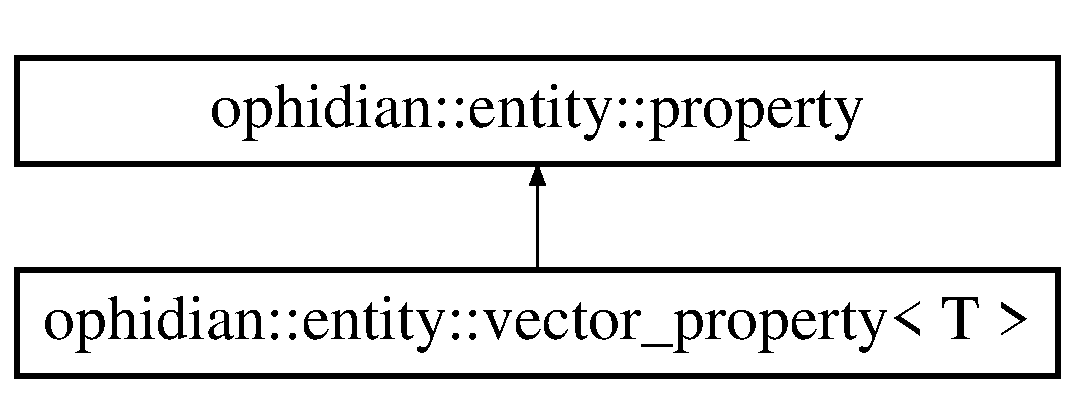
\includegraphics[height=2.000000cm]{classophidian_1_1entity_1_1vector__property}
\end{center}
\end{figure}
\subsection*{Public Member Functions}
\begin{DoxyCompactItemize}
\item 
\hyperlink{classophidian_1_1entity_1_1vector__property_aebd7abc7f2a79b3cfa098ce9be6327dd}{vector\-\_\-property} ()
\begin{DoxyCompactList}\small\item\em Constructor. \end{DoxyCompactList}\item 
void \hyperlink{classophidian_1_1entity_1_1vector__property_a6b239378e987a33fd05c69bd57158bdc}{destroy} (\hyperlink{classophidian_1_1entity_1_1entity}{entity} \&e, std\-::size\-\_\-t index)
\begin{DoxyCompactList}\small\item\em Destroys the property of an entity. \end{DoxyCompactList}\item 
void \hyperlink{classophidian_1_1entity_1_1vector__property_a15ebc0490d8232671cd9111f11351acf}{create} (\hyperlink{classophidian_1_1entity_1_1entity}{entity} \&e, std\-::size\-\_\-t index)
\begin{DoxyCompactList}\small\item\em Creates property for an entity. \end{DoxyCompactList}\item 
T \& \hyperlink{classophidian_1_1entity_1_1vector__property_a2b372566da6796a1db0bd10b42696aec}{operator\mbox{[}$\,$\mbox{]}} (std\-::size\-\_\-t entity\-\_\-index)
\begin{DoxyCompactList}\small\item\em Property getter. \end{DoxyCompactList}\item 
const T \& \hyperlink{classophidian_1_1entity_1_1vector__property_a775e8ebd43e4f32a3f84ffc6b6a025b6}{operator\mbox{[}$\,$\mbox{]}} (std\-::size\-\_\-t entity\-\_\-index) const 
\begin{DoxyCompactList}\small\item\em Constant property getter. \end{DoxyCompactList}\item 
std\-::vector$<$ T $>$\-::const\-\_\-iterator \hyperlink{classophidian_1_1entity_1_1vector__property_a8c6f753870ea6946573d5db86f7ab8c9}{begin} () const 
\begin{DoxyCompactList}\small\item\em Begin iterator. \end{DoxyCompactList}\item 
std\-::vector$<$ T $>$\-::const\-\_\-iterator \hyperlink{classophidian_1_1entity_1_1vector__property_a2f52e3cd85861b854717c64b2d045df8}{end} () const 
\begin{DoxyCompactList}\small\item\em End iterator. \end{DoxyCompactList}\end{DoxyCompactItemize}


\subsection{Detailed Description}
\subsubsection*{template$<$class T$>$class ophidian\-::entity\-::vector\-\_\-property$<$ T $>$}

Describes an implementation of the property class that stores the properties in a vector, acessed by the entity index. 
\begin{DoxyTemplParams}{Template Parameters}
{\em T} & Type of the property value to be stored. \\
\hline
\end{DoxyTemplParams}


\subsection{Constructor \& Destructor Documentation}
\hypertarget{classophidian_1_1entity_1_1vector__property_aebd7abc7f2a79b3cfa098ce9be6327dd}{\index{ophidian\-::entity\-::vector\-\_\-property@{ophidian\-::entity\-::vector\-\_\-property}!vector\-\_\-property@{vector\-\_\-property}}
\index{vector\-\_\-property@{vector\-\_\-property}!ophidian::entity::vector_property@{ophidian\-::entity\-::vector\-\_\-property}}
\subsubsection[{vector\-\_\-property}]{\setlength{\rightskip}{0pt plus 5cm}template$<$class T$>$ {\bf ophidian\-::entity\-::vector\-\_\-property}$<$ T $>$\-::{\bf vector\-\_\-property} (
\begin{DoxyParamCaption}
{}
\end{DoxyParamCaption}
)\hspace{0.3cm}{\ttfamily [inline]}}}\label{classophidian_1_1entity_1_1vector__property_aebd7abc7f2a79b3cfa098ce9be6327dd}
Default constructor. Creates an empty vector property. 

\subsection{Member Function Documentation}
\hypertarget{classophidian_1_1entity_1_1vector__property_a8c6f753870ea6946573d5db86f7ab8c9}{\index{ophidian\-::entity\-::vector\-\_\-property@{ophidian\-::entity\-::vector\-\_\-property}!begin@{begin}}
\index{begin@{begin}!ophidian::entity::vector_property@{ophidian\-::entity\-::vector\-\_\-property}}
\subsubsection[{begin}]{\setlength{\rightskip}{0pt plus 5cm}template$<$class T$>$ std\-::vector$<$T$>$\-::const\-\_\-iterator {\bf ophidian\-::entity\-::vector\-\_\-property}$<$ T $>$\-::begin (
\begin{DoxyParamCaption}
{}
\end{DoxyParamCaption}
) const\hspace{0.3cm}{\ttfamily [inline]}}}\label{classophidian_1_1entity_1_1vector__property_a8c6f753870ea6946573d5db86f7ab8c9}
Returns an iterator pointing to the beginning of the vector of properties. \begin{DoxyReturn}{Returns}
Iterator pointing to the beginning of the vector of properties. 
\end{DoxyReturn}
\hypertarget{classophidian_1_1entity_1_1vector__property_a15ebc0490d8232671cd9111f11351acf}{\index{ophidian\-::entity\-::vector\-\_\-property@{ophidian\-::entity\-::vector\-\_\-property}!create@{create}}
\index{create@{create}!ophidian::entity::vector_property@{ophidian\-::entity\-::vector\-\_\-property}}
\subsubsection[{create}]{\setlength{\rightskip}{0pt plus 5cm}template$<$class T$>$ void {\bf ophidian\-::entity\-::vector\-\_\-property}$<$ T $>$\-::create (
\begin{DoxyParamCaption}
\item[{{\bf entity} \&}]{e, }
\item[{std\-::size\-\_\-t}]{index}
\end{DoxyParamCaption}
)\hspace{0.3cm}{\ttfamily [inline]}, {\ttfamily [virtual]}}}\label{classophidian_1_1entity_1_1vector__property_a15ebc0490d8232671cd9111f11351acf}
Implements the create method from property. Resizes the vector to contain the property of the new entity. 
\begin{DoxyParams}{Parameters}
{\em e} & Entity that was created \\
\hline
{\em index} & The index of the created entity \\
\hline
\end{DoxyParams}


Implements \hyperlink{classophidian_1_1entity_1_1property_a25f0188c1d920cbdb55583772b4817ce}{ophidian\-::entity\-::property}.

\hypertarget{classophidian_1_1entity_1_1vector__property_a6b239378e987a33fd05c69bd57158bdc}{\index{ophidian\-::entity\-::vector\-\_\-property@{ophidian\-::entity\-::vector\-\_\-property}!destroy@{destroy}}
\index{destroy@{destroy}!ophidian::entity::vector_property@{ophidian\-::entity\-::vector\-\_\-property}}
\subsubsection[{destroy}]{\setlength{\rightskip}{0pt plus 5cm}template$<$class T$>$ void {\bf ophidian\-::entity\-::vector\-\_\-property}$<$ T $>$\-::destroy (
\begin{DoxyParamCaption}
\item[{{\bf entity} \&}]{e, }
\item[{std\-::size\-\_\-t}]{index}
\end{DoxyParamCaption}
)\hspace{0.3cm}{\ttfamily [inline]}, {\ttfamily [virtual]}}}\label{classophidian_1_1entity_1_1vector__property_a6b239378e987a33fd05c69bd57158bdc}
Implements the destroy method from property. Moves the last property in the vector to the position of the destroyed entity. 
\begin{DoxyParams}{Parameters}
{\em e} & Entity that was destroyed \\
\hline
{\em index} & The index of the destroyed entity \\
\hline
\end{DoxyParams}


Implements \hyperlink{classophidian_1_1entity_1_1property_a41d49c84d20e3bc9cba0162c9aba6f2b}{ophidian\-::entity\-::property}.

\hypertarget{classophidian_1_1entity_1_1vector__property_a2f52e3cd85861b854717c64b2d045df8}{\index{ophidian\-::entity\-::vector\-\_\-property@{ophidian\-::entity\-::vector\-\_\-property}!end@{end}}
\index{end@{end}!ophidian::entity::vector_property@{ophidian\-::entity\-::vector\-\_\-property}}
\subsubsection[{end}]{\setlength{\rightskip}{0pt plus 5cm}template$<$class T$>$ std\-::vector$<$T$>$\-::const\-\_\-iterator {\bf ophidian\-::entity\-::vector\-\_\-property}$<$ T $>$\-::end (
\begin{DoxyParamCaption}
{}
\end{DoxyParamCaption}
) const\hspace{0.3cm}{\ttfamily [inline]}}}\label{classophidian_1_1entity_1_1vector__property_a2f52e3cd85861b854717c64b2d045df8}
Returns an iterator pointing to the end of the vector of properties. \begin{DoxyReturn}{Returns}
Iterator pointing to the end of the vector of properties. 
\end{DoxyReturn}
\hypertarget{classophidian_1_1entity_1_1vector__property_a2b372566da6796a1db0bd10b42696aec}{\index{ophidian\-::entity\-::vector\-\_\-property@{ophidian\-::entity\-::vector\-\_\-property}!operator\mbox{[}$\,$\mbox{]}@{operator[]}}
\index{operator\mbox{[}$\,$\mbox{]}@{operator[]}!ophidian::entity::vector_property@{ophidian\-::entity\-::vector\-\_\-property}}
\subsubsection[{operator[]}]{\setlength{\rightskip}{0pt plus 5cm}template$<$class T$>$ T\& {\bf ophidian\-::entity\-::vector\-\_\-property}$<$ T $>$\-::operator\mbox{[}$\,$\mbox{]} (
\begin{DoxyParamCaption}
\item[{std\-::size\-\_\-t}]{entity\-\_\-index}
\end{DoxyParamCaption}
)\hspace{0.3cm}{\ttfamily [inline]}}}\label{classophidian_1_1entity_1_1vector__property_a2b372566da6796a1db0bd10b42696aec}
Returns the property value for an entity. 
\begin{DoxyParams}{Parameters}
{\em entity\-\_\-index} & The index of the entity to get the property. \\
\hline
\end{DoxyParams}
\begin{DoxyReturn}{Returns}
A reference to the property of that entity. 
\end{DoxyReturn}
\hypertarget{classophidian_1_1entity_1_1vector__property_a775e8ebd43e4f32a3f84ffc6b6a025b6}{\index{ophidian\-::entity\-::vector\-\_\-property@{ophidian\-::entity\-::vector\-\_\-property}!operator\mbox{[}$\,$\mbox{]}@{operator[]}}
\index{operator\mbox{[}$\,$\mbox{]}@{operator[]}!ophidian::entity::vector_property@{ophidian\-::entity\-::vector\-\_\-property}}
\subsubsection[{operator[]}]{\setlength{\rightskip}{0pt plus 5cm}template$<$class T$>$ const T\& {\bf ophidian\-::entity\-::vector\-\_\-property}$<$ T $>$\-::operator\mbox{[}$\,$\mbox{]} (
\begin{DoxyParamCaption}
\item[{std\-::size\-\_\-t}]{entity\-\_\-index}
\end{DoxyParamCaption}
) const\hspace{0.3cm}{\ttfamily [inline]}}}\label{classophidian_1_1entity_1_1vector__property_a775e8ebd43e4f32a3f84ffc6b6a025b6}
Returns the property value for an entity. Necessary when there is only a constant reference to the properties. 
\begin{DoxyParams}{Parameters}
{\em entity\-\_\-index} & The index of the entity to get the property. \\
\hline
\end{DoxyParams}
\begin{DoxyReturn}{Returns}
A constant reference to the property of that entity. 
\end{DoxyReturn}


The documentation for this class was generated from the following file\-:\begin{DoxyCompactItemize}
\item 
/home/csguth/workspace/openeda/src/entity/vector\-\_\-property.\-h\end{DoxyCompactItemize}

\hypertarget{classophidian_1_1entity_1_1vector__property_3_01bool_01_4}{\section{ophidian\-:\-:entity\-:\-:vector\-\_\-property$<$ bool $>$ Class Template Reference}
\label{classophidian_1_1entity_1_1vector__property_3_01bool_01_4}\index{ophidian\-::entity\-::vector\-\_\-property$<$ bool $>$@{ophidian\-::entity\-::vector\-\_\-property$<$ bool $>$}}
}
Inheritance diagram for ophidian\-:\-:entity\-:\-:vector\-\_\-property$<$ bool $>$\-:\begin{figure}[H]
\begin{center}
\leavevmode
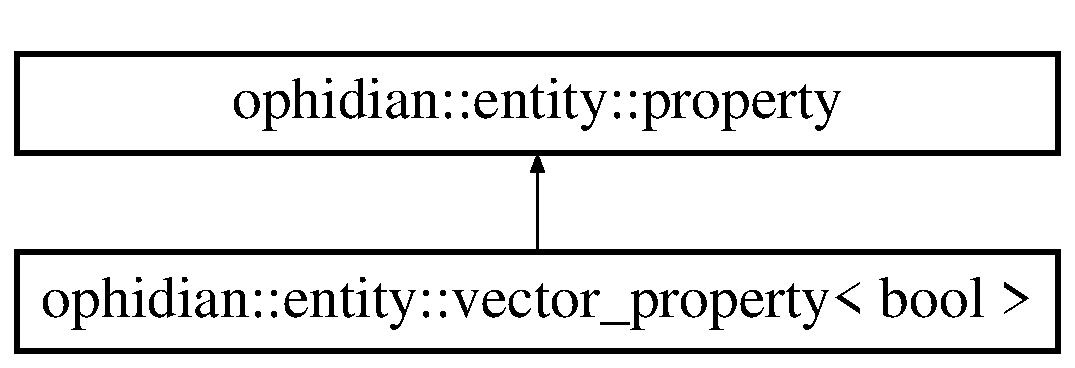
\includegraphics[height=2.000000cm]{classophidian_1_1entity_1_1vector__property_3_01bool_01_4}
\end{center}
\end{figure}
\subsection*{Public Member Functions}
\begin{DoxyCompactItemize}
\item 
void \hyperlink{classophidian_1_1entity_1_1vector__property_3_01bool_01_4_a3d61196d880589d68bf68d81c3310643}{destroy} (\hyperlink{classophidian_1_1entity_1_1entity}{entity} \&e, std\-::size\-\_\-t index)
\begin{DoxyCompactList}\small\item\em Virtual destroy method. \end{DoxyCompactList}\item 
void \hyperlink{classophidian_1_1entity_1_1vector__property_3_01bool_01_4_a3a00eae6f787b0d5cb5b782c931f2774}{create} (\hyperlink{classophidian_1_1entity_1_1entity}{entity} \&e, std\-::size\-\_\-t index)
\begin{DoxyCompactList}\small\item\em Virtual create method. \end{DoxyCompactList}\item 
\hypertarget{classophidian_1_1entity_1_1vector__property_3_01bool_01_4_a8cdce9916803893909c23eda1f4dad74}{std\-::vector$<$ bool $>$\-::reference {\bfseries operator\mbox{[}$\,$\mbox{]}} (std\-::size\-\_\-t entity\-\_\-index)}\label{classophidian_1_1entity_1_1vector__property_3_01bool_01_4_a8cdce9916803893909c23eda1f4dad74}

\item 
\hypertarget{classophidian_1_1entity_1_1vector__property_3_01bool_01_4_ab06b73c923431b61596e25ae6d517852}{bool {\bfseries operator\mbox{[}$\,$\mbox{]}} (std\-::size\-\_\-t entity\-\_\-index) const }\label{classophidian_1_1entity_1_1vector__property_3_01bool_01_4_ab06b73c923431b61596e25ae6d517852}

\item 
\hypertarget{classophidian_1_1entity_1_1vector__property_3_01bool_01_4_a5b73b48445f4a6be9918b0ec98c98c18}{std\-::vector$<$ bool $>$\-::const\-\_\-iterator {\bfseries begin} () const }\label{classophidian_1_1entity_1_1vector__property_3_01bool_01_4_a5b73b48445f4a6be9918b0ec98c98c18}

\item 
\hypertarget{classophidian_1_1entity_1_1vector__property_3_01bool_01_4_a01b33e945c09eccaee7715108fb3b7a2}{std\-::vector$<$ bool $>$\-::const\-\_\-iterator {\bfseries end} () const }\label{classophidian_1_1entity_1_1vector__property_3_01bool_01_4_a01b33e945c09eccaee7715108fb3b7a2}

\end{DoxyCompactItemize}


\subsection{Member Function Documentation}
\hypertarget{classophidian_1_1entity_1_1vector__property_3_01bool_01_4_a3a00eae6f787b0d5cb5b782c931f2774}{\index{ophidian\-::entity\-::vector\-\_\-property$<$ bool $>$@{ophidian\-::entity\-::vector\-\_\-property$<$ bool $>$}!create@{create}}
\index{create@{create}!ophidian::entity::vector_property< bool >@{ophidian\-::entity\-::vector\-\_\-property$<$ bool $>$}}
\subsubsection[{create}]{\setlength{\rightskip}{0pt plus 5cm}void {\bf ophidian\-::entity\-::vector\-\_\-property}$<$ bool $>$\-::create (
\begin{DoxyParamCaption}
\item[{{\bf entity} \&}]{e, }
\item[{std\-::size\-\_\-t}]{index}
\end{DoxyParamCaption}
)\hspace{0.3cm}{\ttfamily [inline]}, {\ttfamily [virtual]}}}\label{classophidian_1_1entity_1_1vector__property_3_01bool_01_4_a3a00eae6f787b0d5cb5b782c931f2774}
This method is called when a new entity is created in the system. 
\begin{DoxyParams}{Parameters}
{\em e} & Entity that was created \\
\hline
{\em index} & The index of the created entity \\
\hline
\end{DoxyParams}


Implements \hyperlink{classophidian_1_1entity_1_1property_a25f0188c1d920cbdb55583772b4817ce}{ophidian\-::entity\-::property}.

\hypertarget{classophidian_1_1entity_1_1vector__property_3_01bool_01_4_a3d61196d880589d68bf68d81c3310643}{\index{ophidian\-::entity\-::vector\-\_\-property$<$ bool $>$@{ophidian\-::entity\-::vector\-\_\-property$<$ bool $>$}!destroy@{destroy}}
\index{destroy@{destroy}!ophidian::entity::vector_property< bool >@{ophidian\-::entity\-::vector\-\_\-property$<$ bool $>$}}
\subsubsection[{destroy}]{\setlength{\rightskip}{0pt plus 5cm}void {\bf ophidian\-::entity\-::vector\-\_\-property}$<$ bool $>$\-::destroy (
\begin{DoxyParamCaption}
\item[{{\bf entity} \&}]{e, }
\item[{std\-::size\-\_\-t}]{index}
\end{DoxyParamCaption}
)\hspace{0.3cm}{\ttfamily [inline]}, {\ttfamily [virtual]}}}\label{classophidian_1_1entity_1_1vector__property_3_01bool_01_4_a3d61196d880589d68bf68d81c3310643}
This method is called when an entity in the system is destroyed. 
\begin{DoxyParams}{Parameters}
{\em e} & Entity that was destroyed \\
\hline
{\em index} & The index of the destroyed entity \\
\hline
\end{DoxyParams}


Implements \hyperlink{classophidian_1_1entity_1_1property_a41d49c84d20e3bc9cba0162c9aba6f2b}{ophidian\-::entity\-::property}.



The documentation for this class was generated from the following file\-:\begin{DoxyCompactItemize}
\item 
/home/csguth/workspace/openeda/src/entity/vector\-\_\-property.\-h\end{DoxyCompactItemize}

\hypertarget{classophidian_1_1timing_1_1wns}{\section{ophidian\-:\-:timing\-:\-:wns Class Reference}
\label{classophidian_1_1timing_1_1wns}\index{ophidian\-::timing\-::wns@{ophidian\-::timing\-::wns}}
}
\subsection*{Public Member Functions}
\begin{DoxyCompactItemize}
\item 
\hypertarget{classophidian_1_1timing_1_1wns_ab74cdcdfb966818119ba6ed8579eb9ed}{{\footnotesize template$<$class P\-Os\-Container , class Wire\-Delay\-Model , class Merge\-Strategy $>$ }\\{\bfseries wns} (const P\-Os\-Container \&P\-Os, const \hyperlink{classophidian_1_1timing_1_1generic__sta}{generic\-\_\-sta}$<$ Wire\-Delay\-Model, Merge\-Strategy $>$ \&sta)}\label{classophidian_1_1timing_1_1wns_ab74cdcdfb966818119ba6ed8579eb9ed}

\item 
\hypertarget{classophidian_1_1timing_1_1wns_a87065c5167909c9f9d7c954e3ab4be9b}{const boost\-::units\-::quantity\\*
$<$ boost\-::units\-::si\-::time $>$ {\bfseries value} () const }\label{classophidian_1_1timing_1_1wns_a87065c5167909c9f9d7c954e3ab4be9b}

\end{DoxyCompactItemize}


The documentation for this class was generated from the following files\-:\begin{DoxyCompactItemize}
\item 
/home/renan/workspace/openeda/src/timing/wns.\-h\item 
/home/renan/workspace/openeda/src/timing/wns.\-cpp\end{DoxyCompactItemize}

%--- End generated contents ---

% Index
\newpage
\phantomsection
\addcontentsline{toc}{chapter}{Index}
\printindex

\end{document}
